% Options for packages loaded elsewhere
\PassOptionsToPackage{unicode}{hyperref}
\PassOptionsToPackage{hyphens}{url}
\PassOptionsToPackage{dvipsnames,svgnames*,x11names*}{xcolor}
%
\documentclass[
  a4paper,
]{article}
\usepackage{lmodern}
\usepackage{amssymb,amsmath}
\usepackage{ifxetex,ifluatex}
\ifnum 0\ifxetex 1\fi\ifluatex 1\fi=0 % if pdftex
  \usepackage[T1]{fontenc}
  \usepackage[utf8]{inputenc}
  \usepackage{textcomp} % provide euro and other symbols
\else % if luatex or xetex
  \usepackage{unicode-math}
  \defaultfontfeatures{Scale=MatchLowercase}
  \defaultfontfeatures[\rmfamily]{Ligatures=TeX,Scale=1}
\fi
% Use upquote if available, for straight quotes in verbatim environments
\IfFileExists{upquote.sty}{\usepackage{upquote}}{}
\IfFileExists{microtype.sty}{% use microtype if available
  \usepackage[]{microtype}
  \UseMicrotypeSet[protrusion]{basicmath} % disable protrusion for tt fonts
}{}
\makeatletter
\@ifundefined{KOMAClassName}{% if non-KOMA class
  \IfFileExists{parskip.sty}{%
    \usepackage{parskip}
  }{% else
    \setlength{\parindent}{0pt}
    \setlength{\parskip}{6pt plus 2pt minus 1pt}}
}{% if KOMA class
  \KOMAoptions{parskip=half}}
\makeatother
\usepackage{xcolor}
\IfFileExists{xurl.sty}{\usepackage{xurl}}{} % add URL line breaks if available
\IfFileExists{bookmark.sty}{\usepackage{bookmark}}{\usepackage{hyperref}}
\hypersetup{
  pdftitle={Analyse de Données},
  pdfauthor={Benoît Simon-Bouhet},
  colorlinks=true,
  linkcolor=Maroon,
  filecolor=Maroon,
  citecolor=Blue,
  urlcolor=blue,
  pdfcreator={LaTeX via pandoc}}
\urlstyle{same} % disable monospaced font for URLs
\usepackage[left=3.75cm, right=3.75cm, top=3cm, bottom=3cm]{geometry}
\usepackage{color}
\usepackage{fancyvrb}
\newcommand{\VerbBar}{|}
\newcommand{\VERB}{\Verb[commandchars=\\\{\}]}
\DefineVerbatimEnvironment{Highlighting}{Verbatim}{commandchars=\\\{\}}
% Add ',fontsize=\small' for more characters per line
\usepackage{framed}
\definecolor{shadecolor}{RGB}{247,247,247}
\newenvironment{Shaded}{\begin{snugshade}}{\end{snugshade}}
\newcommand{\AlertTok}[1]{\textcolor[rgb]{0.75,0.01,0.01}{\textbf{\colorbox[rgb]{0.97,0.90,0.90}{#1}}}}
\newcommand{\AnnotationTok}[1]{\textcolor[rgb]{0.79,0.38,0.79}{#1}}
\newcommand{\AttributeTok}[1]{\textcolor[rgb]{0.00,0.34,0.68}{#1}}
\newcommand{\BaseNTok}[1]{\textcolor[rgb]{0.69,0.50,0.00}{#1}}
\newcommand{\BuiltInTok}[1]{\textcolor[rgb]{0.39,0.29,0.61}{\textbf{#1}}}
\newcommand{\CharTok}[1]{\textcolor[rgb]{0.57,0.30,0.62}{#1}}
\newcommand{\CommentTok}[1]{\textcolor[rgb]{0.54,0.53,0.53}{#1}}
\newcommand{\CommentVarTok}[1]{\textcolor[rgb]{0.00,0.58,1.00}{#1}}
\newcommand{\ConstantTok}[1]{\textcolor[rgb]{0.67,0.33,0.00}{#1}}
\newcommand{\ControlFlowTok}[1]{\textcolor[rgb]{0.12,0.11,0.11}{\textbf{#1}}}
\newcommand{\DataTypeTok}[1]{\textcolor[rgb]{0.00,0.34,0.68}{#1}}
\newcommand{\DecValTok}[1]{\textcolor[rgb]{0.69,0.50,0.00}{#1}}
\newcommand{\DocumentationTok}[1]{\textcolor[rgb]{0.38,0.47,0.50}{#1}}
\newcommand{\ErrorTok}[1]{\textcolor[rgb]{0.75,0.01,0.01}{\underline{#1}}}
\newcommand{\ExtensionTok}[1]{\textcolor[rgb]{0.00,0.58,1.00}{\textbf{#1}}}
\newcommand{\FloatTok}[1]{\textcolor[rgb]{0.69,0.50,0.00}{#1}}
\newcommand{\FunctionTok}[1]{\textcolor[rgb]{0.39,0.29,0.61}{#1}}
\newcommand{\ImportTok}[1]{\textcolor[rgb]{1.00,0.33,0.00}{#1}}
\newcommand{\InformationTok}[1]{\textcolor[rgb]{0.69,0.50,0.00}{#1}}
\newcommand{\KeywordTok}[1]{\textcolor[rgb]{0.12,0.11,0.11}{\textbf{#1}}}
\newcommand{\NormalTok}[1]{\textcolor[rgb]{0.12,0.11,0.11}{#1}}
\newcommand{\OperatorTok}[1]{\textcolor[rgb]{0.12,0.11,0.11}{#1}}
\newcommand{\OtherTok}[1]{\textcolor[rgb]{0.00,0.43,0.16}{#1}}
\newcommand{\PreprocessorTok}[1]{\textcolor[rgb]{0.00,0.43,0.16}{#1}}
\newcommand{\RegionMarkerTok}[1]{\textcolor[rgb]{0.00,0.34,0.68}{\colorbox[rgb]{0.88,0.91,0.97}{#1}}}
\newcommand{\SpecialCharTok}[1]{\textcolor[rgb]{0.24,0.68,0.91}{#1}}
\newcommand{\SpecialStringTok}[1]{\textcolor[rgb]{1.00,0.33,0.00}{#1}}
\newcommand{\StringTok}[1]{\textcolor[rgb]{0.75,0.01,0.01}{#1}}
\newcommand{\VariableTok}[1]{\textcolor[rgb]{0.00,0.34,0.68}{#1}}
\newcommand{\VerbatimStringTok}[1]{\textcolor[rgb]{0.75,0.01,0.01}{#1}}
\newcommand{\WarningTok}[1]{\textcolor[rgb]{0.75,0.01,0.01}{#1}}
\usepackage{longtable,booktabs}
% Correct order of tables after \paragraph or \subparagraph
\usepackage{etoolbox}
\makeatletter
\patchcmd\longtable{\par}{\if@noskipsec\mbox{}\fi\par}{}{}
\makeatother
% Allow footnotes in longtable head/foot
\IfFileExists{footnotehyper.sty}{\usepackage{footnotehyper}}{\usepackage{footnote}}
\makesavenoteenv{longtable}
\usepackage{graphicx,grffile}
\makeatletter
\def\maxwidth{\ifdim\Gin@nat@width>\linewidth\linewidth\else\Gin@nat@width\fi}
\def\maxheight{\ifdim\Gin@nat@height>\textheight\textheight\else\Gin@nat@height\fi}
\makeatother
% Scale images if necessary, so that they will not overflow the page
% margins by default, and it is still possible to overwrite the defaults
% using explicit options in \includegraphics[width, height, ...]{}
\setkeys{Gin}{width=\maxwidth,height=\maxheight,keepaspectratio}
% Set default figure placement to htbp
\makeatletter
\def\fps@figure{htbp}
\makeatother
\setlength{\emergencystretch}{3em} % prevent overfull lines
\providecommand{\tightlist}{%
  \setlength{\itemsep}{0pt}\setlength{\parskip}{0pt}}
\setcounter{secnumdepth}{5}
\usepackage[french]{babel}
\usepackage{fontspec}
% \usepackage{natbib}

% \setallmainfonts[Ligatures = TeX,
                 % ItalicFont={ArcherPro-MediumItalic}]{ArcherPro-Medium}

\usepackage{setspace,booktabs,rotating,placeins,hvfloat,textcomp}

\usepackage{graphicx}
\usepackage{multicol}
\usepackage{enumitem}
\usepackage{longtable}

\setmainfont[Ligatures = TeX]{FuturaLT-Book}
\setmonofont[Scale=0.85]{FiraCode-Regular}
\onehalfspace

\title{Analyse de Données}
\author{Benoît Simon-Bouhet}
\date{2020-08-25}

\begin{document}
\maketitle

{
\hypersetup{linkcolor=}
\setcounter{tocdepth}{2}
\tableofcontents
}
\hypertarget{introduction}{%
\section{Introduction}\label{introduction}}

\hypertarget{objectifs}{%
\subsection{Objectifs}\label{objectifs}}

Ce livre contient l'ensemble du matériel (contenus, exemples, exercices\ldots) nécessaire à la réalisation des travaux pratiques d'analyse de données consacrés à la prise en main de R et RStudio.

Ces travaux pratiques ont essentiellement 3 objectifs :

\begin{enumerate}
\def\labelenumi{\arabic{enumi}.}
\tightlist
\item
  Vous faire (re)découvrir les logiciels \href{https://cran.r-project.org}{R} et \href{https://www.rstudio.com}{Rstudio} dans lesquels vous allez passer beaucoup de temps tout au long de votre cursus de master. Vous avez choisi une spécialité de master qui implique de traiter des données et de communiquer des résultats d'analyses statistiques : R et RStudio devraient être les logiciels vers lesquels vous vous tournez naturellement pour faire l'un et l'autre.
\item
  Vous faire prendre conscience de l'importance des visualisations graphiques :
\end{enumerate}

\begin{itemize}
\tightlist
\item
  d'une part, pour comprendre à quoi ressemblent les données en votre possession,
\item
  d'autre part, pour vous permettre de formuler des hypothèses pertinentes et intéressantes concernant les systèmes que vous étudiez,
\item
  et enfin, pour communiquer efficacement vos trouvailles à un public qui ne connaît pas vos données aussi bien que vous (cela inclut évidemment vos enseignants à l'issue de vos stages).\\
  Les données que vous serez amenés à traiter lors de vos stages, ou plus tard, lorsque vous serez en poste, ont souvent été acquises à grands frais, et au prix d'efforts importants. Il est donc de votre responsabilité d'en tirer le maximum. Et ça commence toujours (ou presque), par la réalisation de visualisations graphiques parlantes.
\end{itemize}

\begin{enumerate}
\def\labelenumi{\arabic{enumi}.}
\setcounter{enumi}{2}
\tightlist
\item
  Vous apprendre comment calculer des statistiques descriptives simples, sur plusieurs types de variables, afin de vous mettre dans les meilleures conditions possibles pour aborder d'une part les statistiques plus avancées de cet EC et des EC des semestres 2 et 3, et d'autre part les comptes-rendus de TP et rapports de stage que vous aurez à produire dans ce cursus de master. Vos enseigants attendent de vous la plus grande rigueur lorsque vous analysez et présentez des résultats d'analyses statistiques. Ces TP ont pour objectifs de vous fournir les bases nécessaires pour satisfaire ce niveau d'exigence.
\end{enumerate}

\begin{center}\rule{0.5\linewidth}{0.5pt}\end{center}

\hypertarget{organisation}{%
\subsection{Organisation}\label{organisation}}

Au total, l'EC d'analyse de données contient :

\begin{itemize}
\tightlist
\item
  15 heures de cours magistraux
\item
  9 heures de travaux pratiques (pour chaque groupe)
\item
  16 heures de TEA
\end{itemize}

\hypertarget{les-cours-magistraux}{%
\subsubsection{Les cours magistraux}\label{les-cours-magistraux}}

Les cours magistraux sont globalement découpés en 2 blocs à peu près indépendants :

\begin{enumerate}
\def\labelenumi{\arabic{enumi}.}
\item
  un bloc de 10 heures consacrées aux notions statistiques élémentaires, aux statistiques descriptives et aux statistiques inférentielles. Nous couvrirons notamment les notions d'incertitude et d'inférence, les tests d'hypothèses, la comparaison de proportions, l'ajustement de données observées à des distributions théoriques, l'analyse de tables de contingences, les comparaisons de moyennes, les régressions linéaires, les ANOVA et ANCOVA\ldots{}
\item
  un bloc de 5 heures consacrées aux statistiques multivariées telles que l'Analyse en Composantes Principales (ACP) et l'Analyse Factorielle des Correspondances (AFC).
\end{enumerate}

Mon objectif n'est pas de survoler l'ensemble du matériel dans ce faible volume horaire : s'il n'est pas suffisant, nous ajouterons quelques séances afin de traiter correctement l'ensemble du matériel. Je suis convaincu que tout le monde est capable de comprendre les grands principes des statistiques, et de réaliser des analyses dans un logiciel tel que R, y compris les plus réfractaires aux mathématiques et à l'informatique. Mais il est nécessaire de démystifier cette discipline essentielle, et si certains ont besoin de plus de temps que d'autres, nous prendrons ce temps. Les TP et TEA, décrits plus bas, sont justement organisés pour permettre à chacun d'avancer à son rythme. Mais ne vous y trompez pas, cela vous demandera \textbf{beaucoup} de travail pendant ces 3 semaines.

Tous les aspects vu en cours seront en effet développés lors des séances de TP et de TEA. Vous aurez, pour chaque partie, des exercices à préparer et à déposer sur l'ENT. Ces exercices seront corrigés lors des séances de TP et/ou de TEA. Tout cela doit d'une part vous préparer à l'évaluation qui aura lieu conjointement avec les EC de stratégie d'échantillonnage, de remise à niveau en biologie marine et d'échantillonnage littoral, mais surtout, cela doit vous permettre d'acquérir des compétences en analyse de données, compétences qui seront attendues de vous lorsque vous sortirez diplômé.e de ce master.

\hypertarget{les-travaux-pratiques}{%
\subsubsection{Les Travaux pratiques}\label{les-travaux-pratiques}}

Le contenu des séances de travaux pratiques sera découpé en 3 parties :

\begin{enumerate}
\def\labelenumi{\arabic{enumi}.}
\tightlist
\item
  Prise en main des logiciels R et RStudio
\item
  Illustration du cours sur les statistiques descriptives et inférentielles, mise en pratique et réalisation d'exercices
\item
  Illustration du cours sur les statistiques multivariées, mise en pratique et réalisation d'exercices
\end{enumerate}

Pour chaque séance de TP, et compte tenu de la situation sanitaire, vous travaillerez soit à distance, soit en salle banalisée, sur vos ordinateurs personnels. La première séance aura lieu en présentiel et sera consacrée à l'installation des logiciels nécessaires à la réalisation des TP ainsi qu'à la présentation de l'organisation des séances.

Les séances de travaux pratiques ne seront \emph{pas toutes obligatoires} : seules quelques séances en présentiel (les dates vous seront présentées ulterieurement) le seront, probablement pas plus d'une par semaine. Pour toutes les autres séances, le fonctionnement sera celui d'une permanence non obligatoire : seuls celles et ceux qui en éprouvent le besoin sont tenus de se déplacer. Ces séances de permanence n'auront lieu que si certains parmi vous m'ont fait part de difficultés ou ont formulé des questions en amont des séances. Si aucune question ne m'a été posée en amont, les permanences n'auront pas lieu. Si une permanence a lieu, elle est ouverte à tous, quel que soit votre groupe de TP. Vous n'êtes d'ailleurs pas tenus de rester pendant 90 minutes : vous venez avec votre question, on y répond ensemble, et vous êtes libres de repartir quand bon vous semble. Les années précédentes, je voyais certains de vos collègues à chaque séance de permanence alors que d'autres ne sont jamais venus. Si vous n'en avez pas besoin, libre à vous de ne pas venir. Tant que le travail est fait et que les exercices ne vous posent pas de problème, vous êtes libres de vous organiser comme vous l'entendez.

Attention toutefois, venir à une séance de permanence en n'ayant pas préparé de question au préalable ne vous sera d'aucune aide. C'est parce que vous avez travaillé en amont de ces séances et que vous arrivez avec des questions que ces permanences sont utiles et efficaces. Donc si vous venez, c'est que vous avez bossé en amont !

\textbf{Comment procéder pour savoir si une séance de permanence a lieu, ou pour poser une question ?}

Tout se passera en ligne, grâce au logiciel \href{https://slack.com/intl/fr-fr/}{Slack}, qui fonctionne un peu comme un ``twitter privé''. Slack facilite la communication des équipes et permet de travailler ensemble. Créez-vous un compte en ligne et installez le logiciel sur votre ordinateur (il existe aussi des versions pour tablettes et smartphones). Lorsque vous aurez installé le logiciel, \href{https://join.slack.com/t/univlrgroupe/shared_invite/zt-grop8wl2-xxV0PNg8DFpVUYmmdk0WAA}{cliquez sur ce lien} pour vous connecter à notre espace de travail commun.

Vous verrez que 3 ``chaînes'' sont disponibles :

\begin{itemize}
\tightlist
\item
  \#organisation : c'est là que les questions liées à l'organisation du cours, des TP et TEA doivent être posées. Si vous ne savez pas si une séance de permanence a lieu, posez la question ici.
\item
  \#rstudio : c'est ici que toutes les questions pratiques liées à l'utilisation de R et RStudio devront êtres posées. Problèmes de syntaxe, problèmes liés à l'interface, à l'installation des packages ou à l'utilisation des fonctions\ldots{} Tout ce qui concerne R ou RStudio mais pas directement les statistiques sera traité ici. Vous êtes libres de poser des questions, de poster des captures d'écran, des morceaux de code, des messages d'erreur. Et vous êtes bien entendus vivement encouragés à vous entraider et à répondre aux questions de vos collègues. Je n'interviendrai ici que pour répondre aux questions laissées sans réponse ou si les réponses apportées sont inexactes. Le fonctionnement est celui d'un forum de discussion instantanné. Vous en tirerez le plus grand bénéfice en participant et en n'ayant pas peur de poser des questions, même si elles vous paraissent idiotes. Rappelez-vous toujours que si vous vous posez une question, d'autres se la posent aussi probablement.
\item
  \#statistiques : c'est ici que toutes les questions liées aux méthodes statistiques devront être posées. Comme pour la chaîne \#rstudio, vous êtes encouragés à poster des questions mais aussi des réponses. Le fonctionnement de l'ensemble se veut participatif.
\end{itemize}

Ainsi, quand vous travaillerez à vos TP ou TEA, prenez l'habitude de garder Slack ouvert sur votre ordinateur. Même si vous n'avez pas de question à poser, votre participation active pour répondre à vos collègues est souhaitable et souhaitée. Votre niveau de participation sur Slack pourra faire partie de votre note finale.

Si toutes les questions posées sur Slack ont trouvé une réponse, alors, inutile d'organiser une permanence. Si en revanche, certains n'ont pas compris, si les mêmes questions reviennent fréquemment, ou si des explications ``en direct'' sont plus efficaces qu'un long message sur Slack, alors une permanence aura lieu.

\hypertarget{le-tea}{%
\subsubsection{Le TEA}\label{le-tea}}

Les séances de TEA auront toutes lieu ``à distance''. Je ne suis pas tenu d'être présent lors des séances de TEA, même si une salle banalisée est systématiquement réservée pour vous permettre de vous retrouver et de travailler ensemble. Je m'engage en revanche à être disponible sur Slack pour répondre rapidement aux questions posées lors des TEA. Et si certaines questions n'ont pas trouvé de réponse pendant les séances de TEA, nous y répondront lors du TP suivant.

Généralement, l'organisation de votre journée sera la suivante :

\begin{enumerate}
\def\labelenumi{\arabic{enumi}.}
\tightlist
\item
  En début de matinée, 1h30 ou 3h de cours magistraux
\item
  En milieu de journée du temps libre ou pour avancer sur ce document, les exercices, la prise en main de R, etc.
\item
  En fin de journée une séance de TEA et/ou de TP/permanence non obligatoire de 90 minutes pour ceux qui en ont besoin et se manifestent.
\end{enumerate}

\hypertarget{luxe9valuation}{%
\subsubsection{L'évaluation}\label{luxe9valuation}}

Vous aurez plusieurs types d'évaluations cette année :

\begin{enumerate}
\def\labelenumi{\arabic{enumi}.}
\item
  Une évaluations par les pairs qui portera sur la qualité de vos scripts. Cette évaluation qui entrera pour une toute petite partie dans la note finale de l'EC a pour objectif principal de vous permettre de vous situer dans vos apprentissages. Vous évaluerez vous même, et de façon anonyme, plusieurs copies de vos camarades en suivant une grille d'évaluation critériée que nous construirons ensemble. De même, votre copie sera évaluée par plusieurs de vos camarades. Cette approche a de nombreux avantages. Elle vous permet notamment de mieux vous approprier les grilles de notations (par exemple, qu'est-ce qu'un bon script sous R ? À l'inverse, qu'est-ce qu'un script médiocre ? Comment être sûr que la méthode statistique choisie est la bonne pour répondre à une question donnée ? Suis-je capable de décrire correctement un tableau de données de grande taille ? Suis-je capable de produire des graphiques informatifs ?) et rends possible un retour personnalisé sur vos travaux beaucoup plus rapidement que si votre enseignant était le seul à corriger l'ensemble de vos travaux. Pas d'inquiétude, vous serez guidés à chaque étape.
\item
  Une évaluation individuelle courte qui ne portera pas sur les analyses statistiques à proprement parler, mais sur votre capacité à produire un graphique de qualité, original et qui raconte une histoire intéressante sur un jeu de données imposé.
\item
  Une évaluation individuelle plus classique avec quelques exercices qui vous demanderont de mettre en œuvre les méthodes statistiques décrites lors de cours magistraux.
\item
  Enfin, une évaluation de groupe qui prendra la forme d'un rapport et qui sera réalisé conjointement avec l'EC de stratégie d'échantillonnage (responsable : Benoît Lebreton). Cet EC est en effet complémentaire de celui d'analyse de données et il sera donc évalués en commun, par un rapport de groupe. En stratégie d'échantillonnage, vous réfléchirez à la meilleure méthode à mettre en œuvre pour collecter des données sur le terrain en vue de répondre à une question scientifique précise. Il vous faudra notamment tenir compte des nombreuses sources de variabilité afin de mettre en œuvre une stratégie adaptée. Vous irez sur le terrain (et au laboratoire) effectuer vous même la collecte de données, et vous analyserez ensuite ces données pour répondre aux questions scientifiques posées initialement. La note d'analyse de données portera donc essentiellement sur les parties ``matériels et méthodes'' et ``résultats'' du rapport commun à ces différents EC que vous aurez à produire. Il est en effet important de comprendre dès maintenant que l'analyse de données n'est pas une fin en soi : on ne fait pas des statistiques pour le plaisir, ou sans but précis. Ça n'est qu'un outil de votre panoplie d'écologue au service d'une question scientifique. L'analyse de données et les statistiques vous permettront de répondre à des questions scientifiques de façon objective, mais leur utilisation appropriée suppose que vous ayez les idées claires en amont sur la question scientifique à laquelle vous tentez de répondre. C'est cette démarche qui devrait vous guider tout au long de votre cursus de master et au-delà, dans votre vie professionnelle.
\end{enumerate}

Dans le cadre de l'approche compétences, j'essaierai d'indiquer, dans la mesure du possible, quelles sont les compétences et résultats d'apprentissages dont vous devrez faire l'acquisition pour chaque évaluation. À l'issue de cet enseignement, vous devriez être capables de :

\begin{enumerate}
\def\labelenumi{\arabic{enumi}.}
\tightlist
\item
  Mettre en forme des données acquises sur le terrain ou au laboratoire afin d'en permettre l'importation dans R ou RStudio.
\item
  Produire des statistiques descriptives informatives permettant de comprendre la structure et les tendances principales d'un jeu de données.
\item
  Créer dans R ou RStudio des graphiques lisibles et informatifs permettant de mettre en évidence les tendances principales d'un jeu de données.
\item
  Produire des scripts clairs sous R ou RStudio, permettant la reproductibilité des traitements de données et des analyses statistiques ainsi que la communication avec vos pairs.
\item
  Analyser des données uni-, bi- ou multi-variées issues d'observations et de mesures sur le terrain et au laboratoire en choisissant les méthodes appropriées pour répondre à une problématique scientifique précise.
\item
  Maîtriser les logiciels R ou RStudio pour réaliser des analyses statistiques, des représentations graphiques ou des simulations numériques.
\end{enumerate}

\hypertarget{bases}{%
\section{R et RStudio : les bases}\label{bases}}

Avant de commencer à explorer des données dans R, il y a plusieurs concepts clés qu'il faut comprendre en premier lieu :

\begin{enumerate}
\def\labelenumi{\arabic{enumi}.}
\tightlist
\item
  Que sont R et RStudio ?
\item
  Comment s'y prend-on pour coder dans R ?
\item
  Que sont les ``packages'' ?
\end{enumerate}

Même si vous pensez être déjà à l'aise avec ces concepts, lisez attentivement ce chapitre et faites les exercices demandés. Cela vous rafraîchira probablement la mémoire, et il n'est pas impossible que vous appreniez une chose ou deux au passage. Une bonne maîtrise des éléments présentés dans ce chapitre est en effet nécessaire pour aborder sereinement les chapitres suivants, à commencer par le chapitre \ref{dataset}, qui présente quelques jeux de données que nous explorerons en détail dans cet ouvrage.

Ce chapitre est en grande partie basé sur les 3 ressources suivantes que je vous encourage à consulter si vous souhaitez obtenir plus de détails :

\begin{enumerate}
\def\labelenumi{\arabic{enumi}.}
\tightlist
\item
  L'ouvrage intitulé \href{https://moderndive.com/index.html}{ModernDive}, de Chester Ismay et Albert Y. Kim. Une bonne partie de ce livre est très largement inspirée de cet ouvrage. C'est en anglais, mais c'est un très bon texte d'introduction aux statistiques sous R et RStudio.
\item
  L'ouvrage intitulé \href{https://ismayc.github.io/rbasics-book/}{Getting used to R, RStudio, and R Markdown} de Chester Ismay, comprend des podcasts (en anglais toujours) que vous pouvez suivre en apprenant.
\item
  Les tutoriels en ligne de DataCamp. DataCamp est une plateforme de e-learning accessible depuis n'importe quel navigateur internet et dont la priorité est l'enseignement des ``data sciences''. Leurs tutoriels vous aideront à apprendre certains des concepts développés dans ce livre. Avant d'aller plus loin, rendez-vous sur \href{https://www.datacamp.com/}{le site de DataCamp} et créez-vous un compte gratuit.
\end{enumerate}

\begin{center}\rule{0.5\linewidth}{0.5pt}\end{center}

\hypertarget{que-sont-r-et-rstudio}{%
\subsection{Que sont R et RStudio}\label{que-sont-r-et-rstudio}}

Pour l'ensemble de ces TP, j'attends de vous que vous utilisiez R \emph{via} RStudio. Les utilisateurs novices confondent souvent les deux. Pour tenter une analogie simple :

\begin{itemize}
\tightlist
\item
  R est le moteur d'une voiture
\item
  RStudio est l'habitacle, le tableau de bord, les pédales
\end{itemize}

Si vous n'avez pas de moteur, vous n'irez nulle part. En revanche, un moteur sans tableau de bord est difficile à manœuvrer. Il est en effet beaucoup plus simple de faire avancer une voiture depuis l'habitacle, plutôt qu'en actionnant à la main les cables et leviers du moteur.

En l'occurence, R est un langage de programmation capable de produire des graphiques et de réaliser des analyses statistiques, des plus simples aux plus complexes. RStudio est un ``emballage'' qui rend l'utilisation de R plus aisée. RStudio est ce qu'on appelle un IDE : Integrated Development Environment. On peut utiliser R sans RStudio, mais c'est nettement plus compliqué, nettement moins pratique.

\hypertarget{installation-de-r-et-rstudio}{%
\subsubsection{Installation de R et RStudio}\label{installation-de-r-et-rstudio}}

\emph{Si vous travaillez exclusivement sur les ordinateurs de l'Université, vous pouvez passer cette section. Si vous souhaitez utiliser R et RStudio sur votre ordinateur personnel, alors suivez le guide !}

Avant tout, vous devez télécharger et installer R et RStudio, dans cet ordre :

\begin{enumerate}
\def\labelenumi{\arabic{enumi}.}
\tightlist
\item
  \href{https://cran.r-project.org}{Téléchargez et installez R}
\end{enumerate}

\begin{itemize}
\tightlist
\item
  Vous devez installer ce logiciel en premier.
\item
  Cliquez sur le lien de téléchargement qui correspond à votre système d'exploitation, puis, sur ``base'', et suivez les instructions.
\end{itemize}

\begin{enumerate}
\def\labelenumi{\arabic{enumi}.}
\setcounter{enumi}{1}
\tightlist
\item
  \href{https://www.rstudio.com/products/RStudio/\#Desktop}{Téléchargez et installez RStudio}
\end{enumerate}

\begin{itemize}
\tightlist
\item
  Cliquez sur ``Download RStudio Desktop''.
\item
  Choisissez la version gratuite et cliquez sur le lien de téléchargement qui correspond à votre système d'exploitation.
\end{itemize}

\hypertarget{utiliser-r-depuis-rstudio}{%
\subsubsection{Utiliser R depuis RStudio}\label{utiliser-r-depuis-rstudio}}

Puisqu'il est beaucoup plus facile d'utiliser Rstudio pour interagir avec R, nous utiliserons exclusivement l'interface de RStudio. Après l'installation des 2 logiciels, vous disposez de 2 nouveaux logiciels sur votre ordinateur. RStudio ne peut fonctionner sans R, mais nous travaillerons exclusivement dans RStudio :

\begin{itemize}
\tightlist
\item
  R, ne pas ouvrir ceci : 
\includegraphics{images/Rlogo.png}
\item
  RStudio, ouvrir ça : 
\includegraphics{images/RStudio-Ball.png}
\end{itemize}

À l'université, vous trouverez RStudio dans le menu Windows. Quand vous ouvrez RStudio pour la première fois, vous devriez obtenir une fenêtre qui ressemble à ceci :

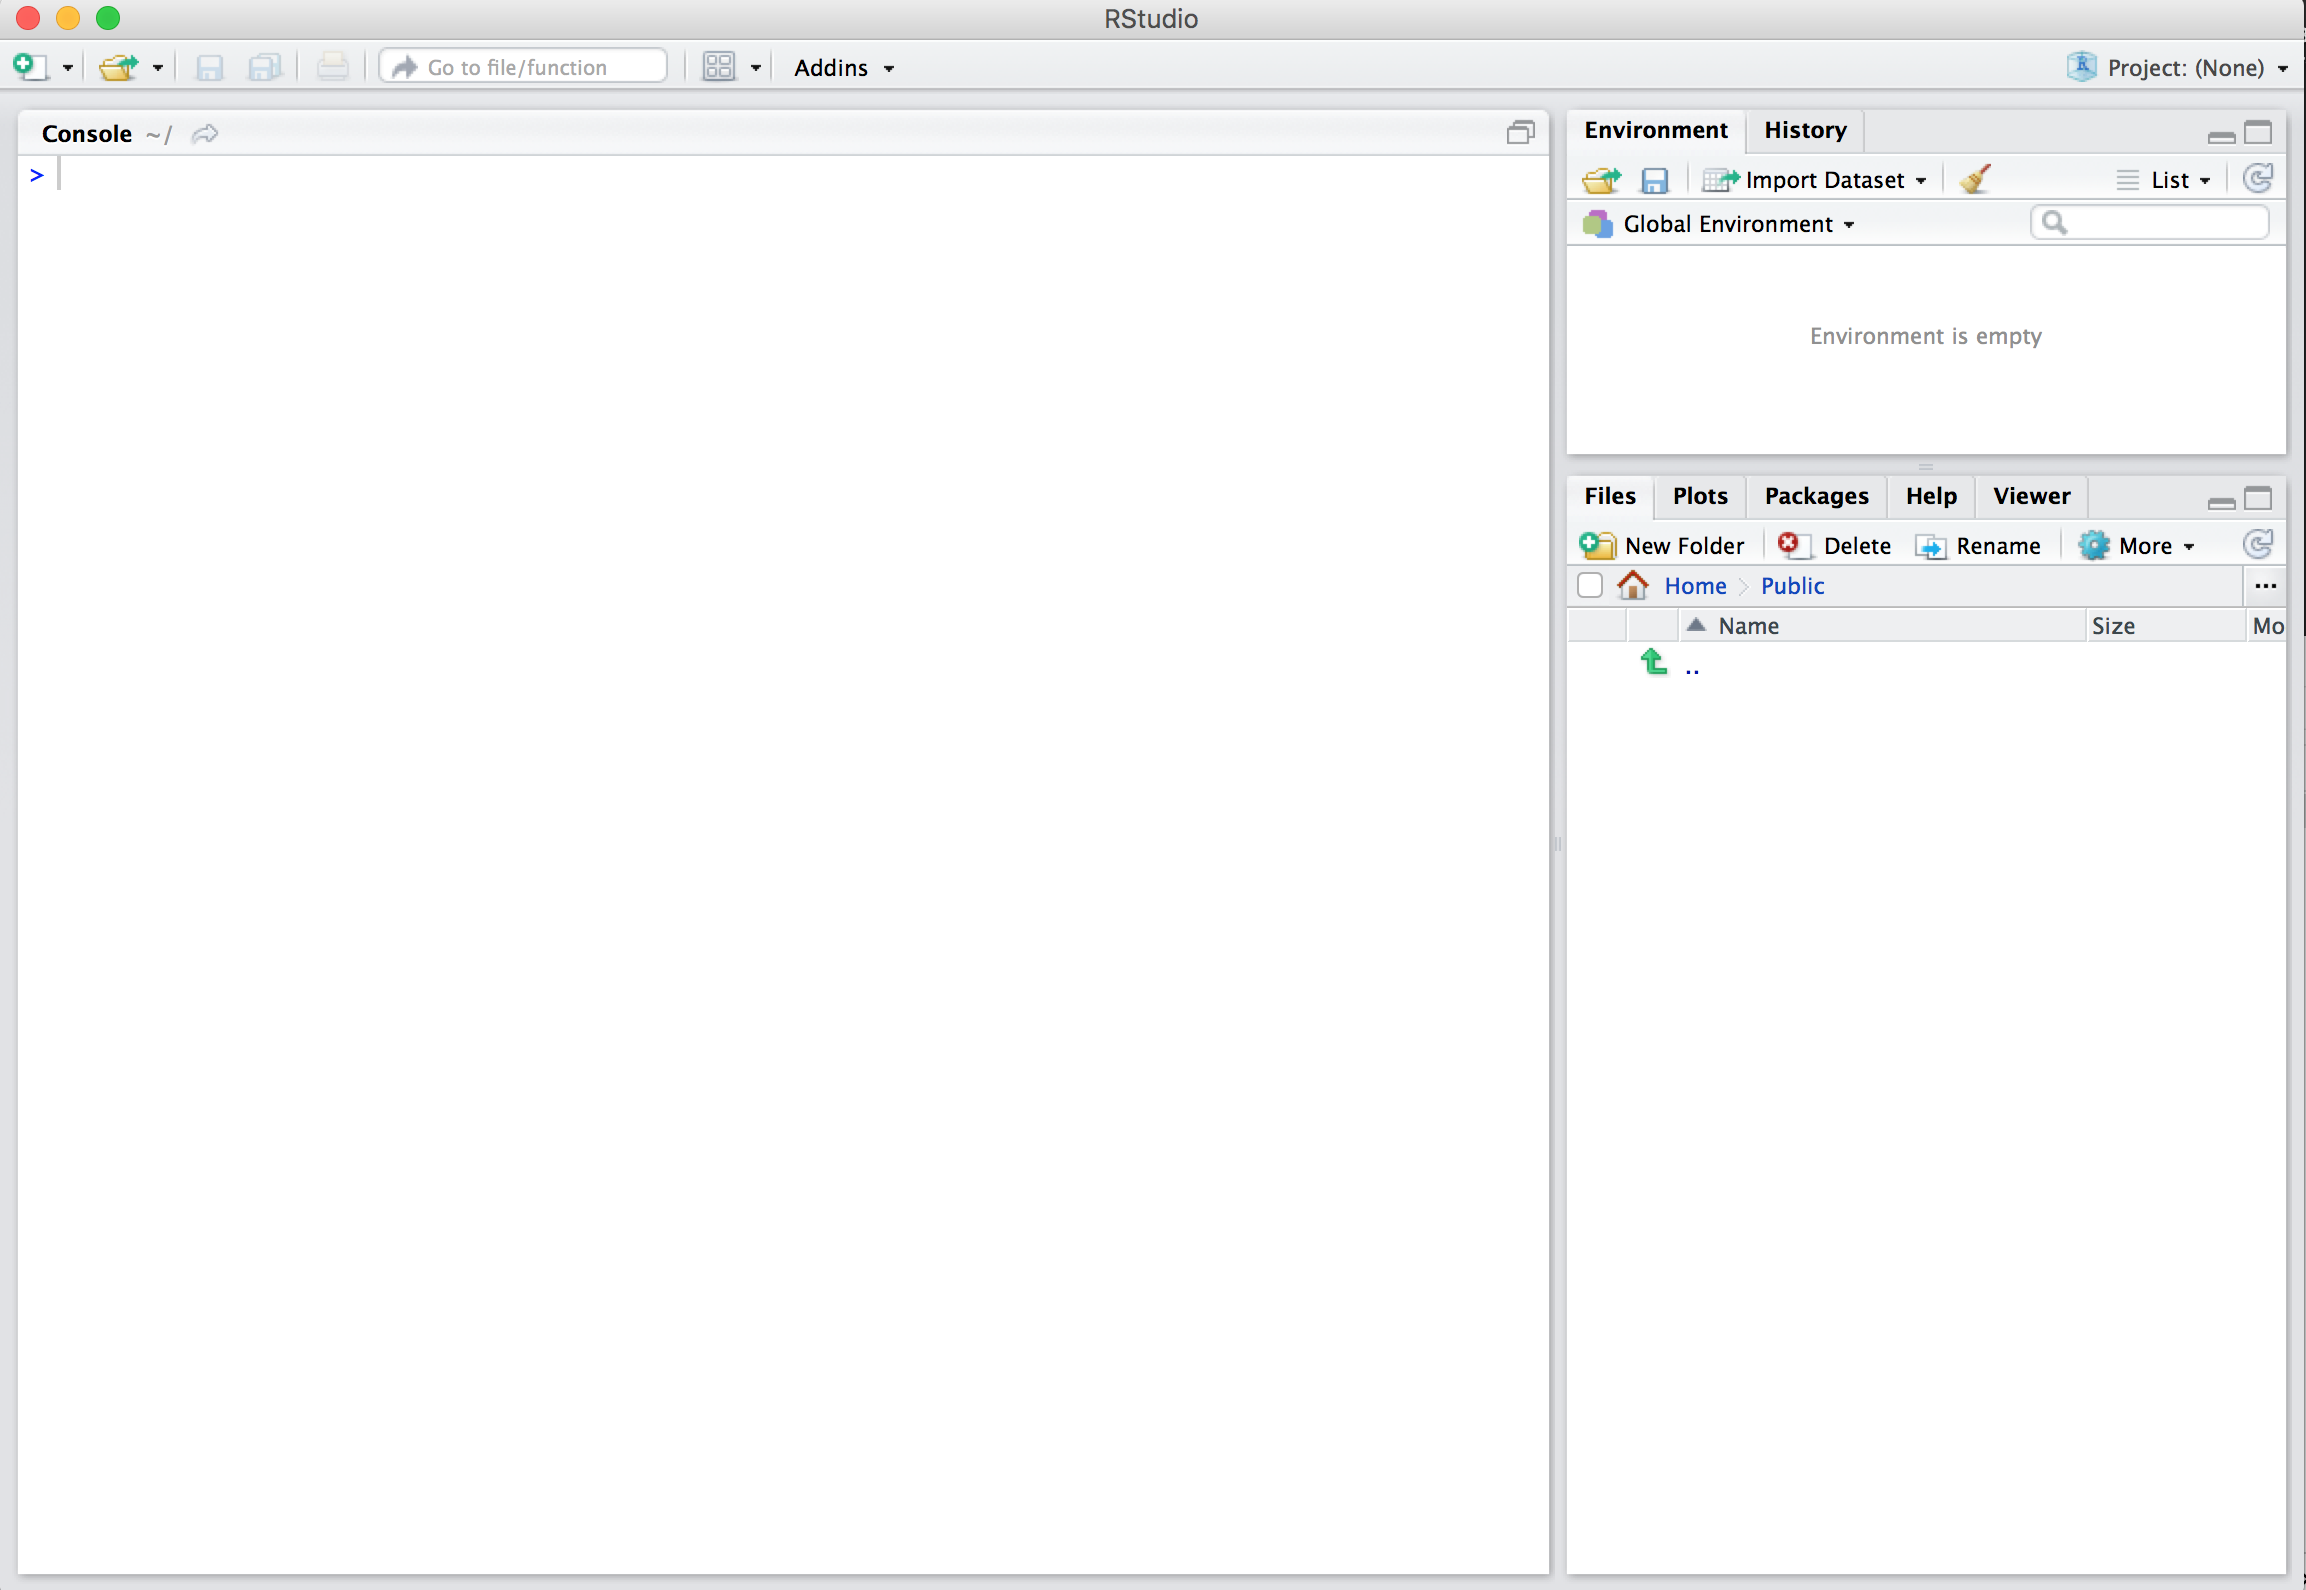
\includegraphics{images/rstudio.png}

Prenez le temps d'explorer cette interface, cliquez sur les différents onglets, ouvrez les menus, allez faire un tour dans les préférences du logiciel pour découvrir les différents panneaux de l'application, en particulier la Console dans laquelle nous exécuterons très bientôt du code R.

\begin{center}\rule{0.5\linewidth}{0.5pt}\end{center}

\hypertarget{code}{%
\subsection{Comment exécuter du code R ?}\label{code}}

Maintenant que vous avez installé R et RStudio, vous vous demandez probablement comment on s'en sert\ldots{} La première chose à noter est que, contrairement à d'autres logiciels comme Excel, STATA ou SAS qui fournissent des interfaces où tout se fait en cliquant avec sa souris, R est un langage interprété, ce qui signifie que vous devez taper des commandes R, écrites en code R. C'est-à-dire que vous devez \textbf{programmer} en R (j'utilise les termes ``coder'' et ``programmer'' de manière interchangeable dans ce livre).

Il n'est pas nécessaire d'être un programmeur pour utiliser R, néanmoins, il est nécessaire de programmer ! Il existe en effet un ensemble de concepts de programmation de base que les utilisateurs de R doivent comprendre et maîtriser. Par conséquent, bien que ce livre ne soit pas un livre sur la programmation, vous en apprendrez juste assez en programmation pour explorer et analyser efficacement des données.

\hypertarget{la-console}{%
\subsubsection{La console}\label{la-console}}

La façon la plus simle d'interagir avec RStudio (mais pas du tout la meilleure !) consiste à taper directement des commandes que R pourra comprendre dans la Console.

Cliquez dans la console (après le symbole \texttt{\textgreater{}}) et tapez ceci, sans oublier de valider en tapant sur la touche \texttt{Entrée} :

\begin{Shaded}
\begin{Highlighting}[]
\DecValTok{3} \OperatorTok{+}\StringTok{ }\DecValTok{8}
\end{Highlighting}
\end{Shaded}

\begin{verbatim}
[1] 11
\end{verbatim}

Félicitations, vous venez de taper votre première instruction R : vous savez maintenant faire des additions !

\hypertarget{le-ruxe9pertoire-de-travail}{%
\subsubsection{Le répertoire de travail}\label{le-ruxe9pertoire-de-travail}}

La première commande que vous devriez connaître quand vous travaillez dans R ou RStudio est la suivante :

\begin{Shaded}
\begin{Highlighting}[]
\KeywordTok{getwd}\NormalTok{()}
\end{Highlighting}
\end{Shaded}

Si vous tapez cette commande dans la console, RStudio doit vous afficher un emplacement sur votre ordinateur. Cet emplacement est appelé ``Répertoire de travail'', ou ``Working Directory'' en anglais (\texttt{getwd()} est l'abbréviation de ``Get Working Directory'').

Ce répertoire de travail est important : c'est là que seront stockés les tableaux et graphiques que vous déciderez de sauvegarder. C'est là aussi que vous sauvegarderez vos scripts (voir plus bas) qui vous permettront de garder la trace de votre travail et de le reprendre là où vous l'aviez laissé la dernière fois. Enfin, lorsque vous souhaiterez importer des tableaux de données contenus dans des fichiers externes (par exemple, des fichiers Excel), c'est également dans ce répertoire que R tentera de trouver vos données.

Avant d'aller plus loin je vous conseille donc vivement de :

\begin{enumerate}
\def\labelenumi{\arabic{enumi}.}
\tightlist
\item
  Créer un nouveau dossier intitulé ``Rstats'' sur votre espace personnel (généralement, sur le disque ``W:'' des ordinateurs de l'Université)
\item
  Indiquez à RStudio que vous souhaitez travailler dans ce nouveau répertoire de travail. Pour cela vous avez 3 solutions au choix :

  \begin{enumerate}
  \def\labelenumii{\arabic{enumii}.}
  \tightlist
  \item
    Dans RStudio, cliquez dans le menu ``Session \textgreater{} Set Working Directory \textgreater{} Choose Directory\ldots{}'' puis naviguez jusqu'au dossier que vous venez de créer
  \item
    Dans le panneau ``Files'', naviguez jusqu'au dossier ``Rstats'' que vous venez de créer, puis cliquez sur le bouton ``More \textgreater{} Set As Working Directory''
  \item
    En ligne de commande, dans la console, utilisez la fonction \texttt{setwd()} pour spécifier le chemin de votre nouveau dossier, par exemple :
  \end{enumerate}
\end{enumerate}

\begin{Shaded}
\begin{Highlighting}[]
\CommentTok{# Attention à bien respecter les majuscules et à utiliser les}
\CommentTok{# guillemets.}
\KeywordTok{setwd}\NormalTok{(}\StringTok{"W:/Rstats"}\NormalTok{)}
\end{Highlighting}
\end{Shaded}

Il ne vous reste plus qu'à vérifier que le changement a bien été pris en compte en tapant à nouveau \texttt{getwd()} dans la console. Attention, vous devrez vous assurer d'être dans le bon répertoire de travail \textbf{à chaque nouvelle session} !

\hypertarget{les-scripts}{%
\subsubsection{Les scripts}\label{les-scripts}}

Taper du code directement dans la console est probablement la pire façon de travailler dans RStudio. Cela est parfois utile pour faire un rapide calcul, ou pour vérifier qu'une commande fonctionne correctement. Mais la plupart du temps, vous devriez taper vos commandes dans un script.

Un script est un fichier au format ``texte brut'' (cela signifie qu'il n'y a pas de mise en forme et que ce fichier peut-être ouvert par n'importe quel éditeur de texte, y compris les plus simples comme le bloc notes de Windows), dans lequel vous pouvez taper :

\begin{enumerate}
\def\labelenumi{\arabic{enumi}.}
\tightlist
\item
  des instructions qui seront comprises par R comme si vous les tapiez directement dans la console
\item
  des lignes de commentaires, qui doivent obligatoirement commencer par le symbole \texttt{\#}.
\end{enumerate}

Les avantages de travailler dans un script sont nombreux :

\begin{enumerate}
\def\labelenumi{\arabic{enumi}.}
\tightlist
\item
  Vous pouvez sauvegarder votre script à tout moment (vous devriez prendre l'habitude de le sauvegarder très régulièrement). Vous gardez ainsi la trace de toutes les commandes que vous avez tapées.
\item
  Vous pouvez aisément partager votre script pour collaborer avec vos collègues de promo et enseignants.
\item
  Vous pouvez documenter votre démarche et les différentes étapes de vos analyses. Vous devez ajouter autant de commentaires que possible. Cela permettra à vos collaborateurs de comprendre ce que vous avez fait. Et dans 6 mois, cela vous permettra de comprendre ce que vous avez fait. Si votre démarche vous paraît cohérente aujourd'hui, il n'est en effet pas garanti que vous vous souviendrez de chaque détail quand vous vous re-plongerez dans vos analyses dans quelques temps. Donc aidez-vous vous même en commentant vos scripts dès maintenant.
\item
  Un script bien structuré, bien indenté (avec les bons retours à la ligne, des sauts de lignes, des espaces, bref, de l'air) et clair permet de rendre vos analyses répétables. Si vous passez 15 heures à analyser un tableau de données précis, il vous suffira de quelques secondes pour analyser un nouveau jeu de données similaire : vous n'aurez que quelques lignes à modifier dans votre script original pour l'appliquer à de nouvelles données.
\end{enumerate}

Vous pouvez créer un script en cliquant dans le menu ``File \textgreater{} New File \textgreater{} R Script''. Un nouveau panneau s'ouvre dans l'application. Pensez à sauvegarder immédiatement votre nouveau script. Il faut pour cela lui donner un nom. Vous noterez que par défaut, RStudio propose d'enregistrer votre script dans votre répertoire de travail.

À partir de maintenant, vous ne devriez plus taper de commande directement dans la console. Tapez systématiquement vos commandes dans un script et sauvegardez-le régulièrement.

Pour exécuter les commandes du script dans la console, il suffit de placer le curseur sur la ligne contenant la commande et de presser les touches \texttt{ctrl\ +\ enter} (ou \texttt{command\ +\ enter} sous macOS). Si un message d'erreur s'affiche dans la console, c'est que votre instruction était erronée. Modifiez la directement dans votre script et pressez à nouveau les touches \texttt{ctrl\ +\ enter} (ou \texttt{command\ +\ enter} sous macOS) pour tenter à nouveau votre chance. Idéalement, votre script ne devrait contenir que des commandes qui fonctionnent et des commentaires expliquant à quoi servent ces commandes.

Ci-dessous, un exemple de script :

\begin{Shaded}
\begin{Highlighting}[]
\CommentTok{# Penser à installer le package ggplot2 si besoin}
\CommentTok{# install.packages("ggplot2")}

\CommentTok{# Chargement du package}
\KeywordTok{library}\NormalTok{(ggplot2)}

\CommentTok{# Mise en mémoire des données de qualité de l'air à New-York de mai à}
\CommentTok{# septembre 1973}
\KeywordTok{data}\NormalTok{(airquality)}

\CommentTok{# Affichage des premières lignes du tableau de données}
\KeywordTok{head}\NormalTok{(airquality)}

\CommentTok{# Quelle est la structure de ce tableau ?}
\KeywordTok{str}\NormalTok{(airquality)}

\CommentTok{# Réalisation d'un graphique présentant la relation entre la concentration}
\CommentTok{# en ozone atmosphérique en ppb et la température en degrés Farenheit}
\KeywordTok{ggplot}\NormalTok{(}\DataTypeTok{data =}\NormalTok{ airquality, }\DataTypeTok{mapping =} \KeywordTok{aes}\NormalTok{(}\DataTypeTok{x =}\NormalTok{ Temp, }\DataTypeTok{y =}\NormalTok{ Ozone)) }\OperatorTok{+}
\StringTok{  }\KeywordTok{geom_point}\NormalTok{() }\OperatorTok{+}
\StringTok{  }\KeywordTok{geom_smooth}\NormalTok{(}\DataTypeTok{method =} \StringTok{"loess"}\NormalTok{)}

\CommentTok{# On constate une augmentation importante de la concentration d'ozone }
\CommentTok{# pour des températures supérieures à 75ºF}
\end{Highlighting}
\end{Shaded}

Même si vous ne comprenez pas encore les commandes qui figurent dans ce script (ça viendra !), voici ce que vous devez en retenir :

\begin{enumerate}
\def\labelenumi{\arabic{enumi}.}
\tightlist
\item
  Le script contient plus de lignes de commentaires que de commandes R.
\item
  Chaque étape de l'analyse est décrite en détail.
\item
  On peut ajouter des commentaires afin de décrire les résultats.
\item
  Seules les commandes pertinentes et qui fonctionnent ont été conservées dans ce script.
\item
  Chaque ligne de commentaire commence par \texttt{\#}. Il est ainsi possible de conserver certaines commandes R dans le script, ``pour mémoire'', sans pour autant qu'elle ne soient exécutées. C'est le cas pour la ligne \texttt{\#\ install.packages("ggplot2")}.
\end{enumerate}

Si j'exécute ce script dans la console de RStudio (en sélectionnant toutes les lignes et en pressant les touches \texttt{ctrl\ +\ enter} ou \texttt{command\ +\ enter} sous macOS), voilà ce qui est produit :

\begin{verbatim}
  Ozone Solar.R Wind Temp Month Day
1    41     190  7.4   67     5   1
2    36     118  8.0   72     5   2
3    12     149 12.6   74     5   3
4    18     313 11.5   62     5   4
5    NA      NA 14.3   56     5   5
6    28      NA 14.9   66     5   6
\end{verbatim}

\begin{verbatim}
'data.frame':   153 obs. of  6 variables:
 $ Ozone  : int  41 36 12 18 NA 28 23 19 8 NA ...
 $ Solar.R: int  190 118 149 313 NA NA 299 99 19 194 ...
 $ Wind   : num  7.4 8 12.6 11.5 14.3 14.9 8.6 13.8 20.1 8.6 ...
 $ Temp   : int  67 72 74 62 56 66 65 59 61 69 ...
 $ Month  : int  5 5 5 5 5 5 5 5 5 5 ...
 $ Day    : int  1 2 3 4 5 6 7 8 9 10 ...
\end{verbatim}

\begin{center}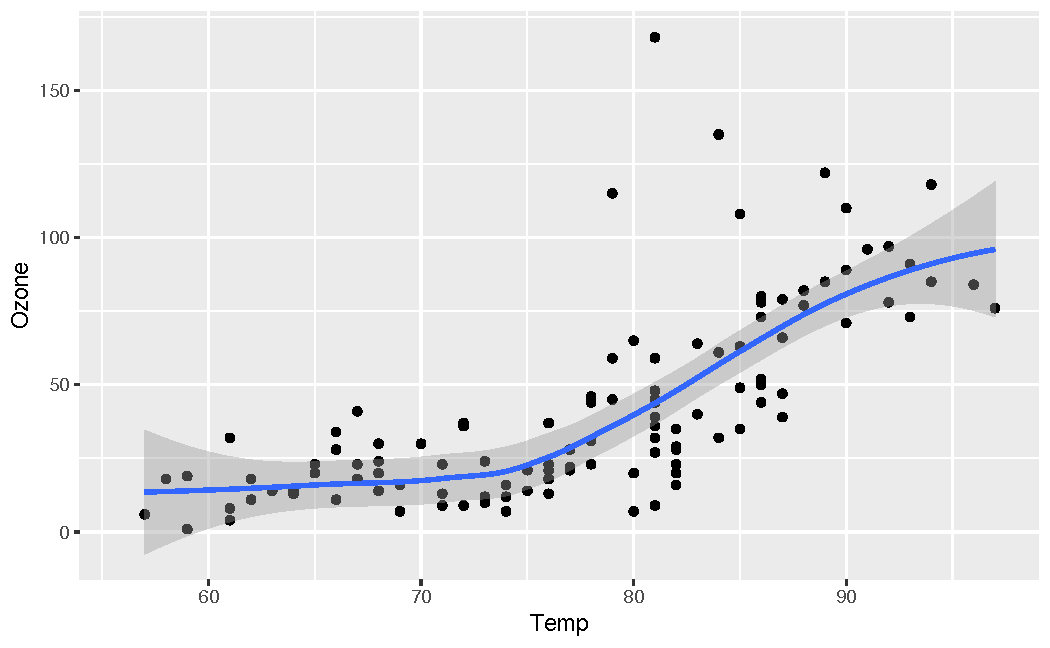
\includegraphics[width=0.9\linewidth]{figure/unnamed-chunk-5-1} \end{center}

\hypertarget{concepts-de-base-en-programmation-et-terminologie}{%
\subsubsection{Concepts de base en programmation et terminologie}\label{concepts-de-base-en-programmation-et-terminologie}}

Pour vous présenter les concepts de base et la terminologie de la programmation dont nous aurons besoin dans R, vous allez suivre des tutoriels en ligne sur le site de DataCamp. Pour chacun des tutoriels, j'indique une liste des concepts de programmation couverts. Notez que dans ce livre, nous utiliserons une police différente pour distinguer le texte normal et les \texttt{commandes-informatiques}.

Il est important de noter que, bien que ces tutoriels sont d'excellentes introductions, une seule lecture est insuffisante pour un apprentissage en profondeur et une rétention à long terme. Les outils ultimes pour l'apprentissage et la rétention à long terme sont ``l'apprentissage par la pratique'' et ``la répétition''. Outre les exercices demandés dans DataCamp, que vous devez effectuer directement dans votre navigateur, je vous encourage donc à multiplier les essais, directement dans la console de RStudio, ou, de préférence, dans un script que vous annoterez, pour vous assurer que vous avez bien compris chaque partie.

\hypertarget{objects}{%
\paragraph{Objets, types, vecteurs, facteurs et tableaux de données}\label{objects}}

Dans \href{https://www.datacamp.com/community/open-courses/introduction-a-r}{le cours d'introduction à R} sur DataCamp, suivez les chapitres suivants. Au fur et à mesure de votre travail, notez les termes importants et ce à quoi ils font référence.

\begin{itemize}
\tightlist
\item
  \href{https://campus.datacamp.com/courses/introduction-a-r/chapitre-1-introduction?ex=1}{Chapitre 1 : introduction}

  \begin{itemize}
  \tightlist
  \item
    La console : l'endroit où vous tapez des commandes.
  \item
    Les objets : où les valeurs sont stockées, comment assigner des valeurs à des objets.
  \item
    Les types de données : entiers, doubles/numériques, charactères et logiques.
  \end{itemize}
\item
  \href{https://campus.datacamp.com/courses/introduction-a-r/chapitre-2-les-vecteurs?ex=1}{Chapitre 2 : vecteurs}

  \begin{itemize}
  \tightlist
  \item
    Les vecteurs : des collections de valeurs du même type.
  \end{itemize}
\item
  \href{https://campus.datacamp.com/courses/introduction-a-r/chapitre-4-facteurs?ex=1}{Chapitre 4 : les facteurs}

  \begin{itemize}
  \tightlist
  \item
    Des données catégorielles (et non pas \emph{numériques}) représentées dans R sous forme de \texttt{factor}s.
  \end{itemize}
\item
  \href{https://campus.datacamp.com/courses/introduction-a-r/chapitre-5-les-jeux-de-donnees?ex=1}{Chapitre 5 : les jeux de données ou \texttt{data.frame}}

  \begin{itemize}
  \tightlist
  \item
    Les \texttt{data.frame}s sont similaires aux feuilles de calcul rectangulaires que l'on peut produire dans un tableur. Dans R, ce sont des objets rectangulaires (des tableaux !) contenant des jeux de données : les lignes correspondent aux observations et les colonnes aux variables décrivant les observations. La plupart du temps, c'est le format de données que nous utiliserons. Plus de détails dans le chapitre \ref{dataset}.
  \end{itemize}
\end{itemize}

Avant de passer à la suite, il nous reste 2 grandes notions à découvrir dans le domaine du code et de la syntaxe afin de pouvoir travailler efficacement dans R : les opérateurs de comparaison d'une part, et les fonctions d'autre part.

\hypertarget{comparaison}{%
\paragraph{Opérateurs de comparaison}\label{comparaison}}

Comme leur nom l'indique, ils permettent de comparer des valeurs ou des objets. Les principaux opérateurs de comparaison sont :

\begin{itemize}
\tightlist
\item
  \texttt{==} : égal à
\item
  \texttt{!=} : différent de
\item
  \texttt{\textgreater{}} : supérieur à
\item
  \texttt{\textless{}} : inférieur à
\item
  \texttt{\textgreater{}=} : supérieur ou égal à
\item
  \texttt{\textless{}=} : inférieur ou égal à
\end{itemize}

Ainsi, on peut tester si 3 est égal à 5 :

\begin{Shaded}
\begin{Highlighting}[]
\DecValTok{3} \OperatorTok{==}\StringTok{ }\DecValTok{5}
\end{Highlighting}
\end{Shaded}

\begin{verbatim}
[1] FALSE
\end{verbatim}

La réponse est bien entendu \texttt{FALSE}. Est-ce que 3 est inférieur à 5 ?

\begin{Shaded}
\begin{Highlighting}[]
\DecValTok{3} \OperatorTok{<}\StringTok{ }\DecValTok{5}
\end{Highlighting}
\end{Shaded}

\begin{verbatim}
[1] TRUE
\end{verbatim}

La réponse est maintenant \texttt{TRUE}. Lorsque l'on utilise un opérateur de comparaison, la réponse est toujours soit vrai (\texttt{TRUE}), soit faux (\texttt{FALSE}).

Il est aussi possible de comparer des chaînes de charactères :

\begin{Shaded}
\begin{Highlighting}[]
\StringTok{"Bonjour"} \OperatorTok{==}\StringTok{ "Au revoir"}
\end{Highlighting}
\end{Shaded}

\begin{verbatim}
[1] FALSE
\end{verbatim}

\begin{Shaded}
\begin{Highlighting}[]
\StringTok{"Bonjour"} \OperatorTok{>=}\StringTok{ "Au revoir"}
\end{Highlighting}
\end{Shaded}

\begin{verbatim}
[1] TRUE
\end{verbatim}

Manifestement, ``Bonjour'' est supérieur ou égal à ``Au revoir''. En fait, R utilise l'ordre alphabétique pour comparer les chaînes de caractères. Puisque dans l'alphabet, le ``B'' de ``Bonjour'' arrive après le ``A'' de ``Au revoir'', pour R, ``Bonjour'' est supérieur à ``Au revoir''.

Il est également possible d'utiliser ces opérateurs pour comparer un chiffre et un vecteur :

\begin{Shaded}
\begin{Highlighting}[]
\NormalTok{tailles_pop1 <-}\StringTok{ }\KeywordTok{c}\NormalTok{(}\DecValTok{112}\NormalTok{, }\DecValTok{28}\NormalTok{, }\DecValTok{86}\NormalTok{, }\DecValTok{14}\NormalTok{, }\DecValTok{154}\NormalTok{, }\DecValTok{73}\NormalTok{, }\DecValTok{63}\NormalTok{, }\DecValTok{48}\NormalTok{)}
\NormalTok{tailles_pop1 }\OperatorTok{>}\StringTok{ }\DecValTok{80}
\end{Highlighting}
\end{Shaded}

\begin{verbatim}
[1]  TRUE FALSE  TRUE FALSE  TRUE FALSE FALSE FALSE
\end{verbatim}

Ici, l'opérateur nous permet d'identifier quels éléments du vecteur \texttt{taille\_pop1} sont supérieurs à 80. Il s'agit des éléments placés en première, troisième et cinquième positions.

Il est aussi possible de comparer 2 vecteurs qui contiennent le même nombre d'éléments :

\begin{Shaded}
\begin{Highlighting}[]
\NormalTok{tailles_pop2 <-}\StringTok{ }\KeywordTok{c}\NormalTok{(}\DecValTok{114}\NormalTok{, }\DecValTok{27}\NormalTok{, }\DecValTok{38}\NormalTok{, }\DecValTok{91}\NormalTok{, }\DecValTok{54}\NormalTok{, }\DecValTok{83}\NormalTok{, }\DecValTok{33}\NormalTok{, }\DecValTok{68}\NormalTok{)}
\NormalTok{tailles_pop1 }\OperatorTok{>}\StringTok{ }\NormalTok{tailles_pop2}
\end{Highlighting}
\end{Shaded}

\begin{verbatim}
[1] FALSE  TRUE  TRUE FALSE  TRUE FALSE  TRUE FALSE
\end{verbatim}

Les comparaisons sont ici faites élément par élément. Ainsi, les observations 2, 3, 5 et 7 du vecteur \texttt{tailles\_pop1} sont supérieures aux observations 2, 3, 5 et 7 du vecteur \texttt{tailles\_pop2} respectivement.

Ces vecteurs de vrais/faux sont très utiles car ils peuvent permettre de compter le nombre d'éléments répondant à une certains condition :

\begin{Shaded}
\begin{Highlighting}[]
\KeywordTok{sum}\NormalTok{(tailles_pop1 }\OperatorTok{>}\StringTok{ }\NormalTok{tailles_pop2)}
\end{Highlighting}
\end{Shaded}

\begin{verbatim}
[1] 4
\end{verbatim}

Lorsque l'on effectue une opération arithmétique (comme le calcul d'une somme ou d'une moyenne) sur un vecteur de vrais/faux, les \texttt{TRUE} sont remplacés par \texttt{1} et les \texttt{FALSE} par \texttt{0}. La somme nous indique donc le nombre de vrais dans un vecteur de vrais/faux, et la moyenne nous indique la proportion de vrais :

\begin{Shaded}
\begin{Highlighting}[]
\KeywordTok{mean}\NormalTok{(tailles_pop1 }\OperatorTok{>}\StringTok{ }\NormalTok{tailles_pop2)}
\end{Highlighting}
\end{Shaded}

\begin{verbatim}
[1] 0.5
\end{verbatim}

\textbf{Note} : Attention, si les vecteurs comparés n'ont pas la même taille, un message d'avertissement est affiché :

\begin{Shaded}
\begin{Highlighting}[]
\NormalTok{tailles_pop3 <-}\StringTok{ }\KeywordTok{c}\NormalTok{(}\DecValTok{43}\NormalTok{, }\DecValTok{56}\NormalTok{, }\DecValTok{92}\NormalTok{)}
\NormalTok{tailles_pop1}
\end{Highlighting}
\end{Shaded}

\begin{verbatim}
[1] 112  28  86  14 154  73  63  48
\end{verbatim}

\begin{Shaded}
\begin{Highlighting}[]
\NormalTok{tailles_pop3}
\end{Highlighting}
\end{Shaded}

\begin{verbatim}
[1] 43 56 92
\end{verbatim}

\begin{Shaded}
\begin{Highlighting}[]
\NormalTok{tailles_pop3 }\OperatorTok{>}\StringTok{ }\NormalTok{tailles_pop1}
\end{Highlighting}
\end{Shaded}

\begin{verbatim}
Warning in tailles_pop3 > tailles_pop1: la taille d'un objet plus long
n'est pas multiple de la taille d'un objet plus court
\end{verbatim}

\begin{verbatim}
[1] FALSE  TRUE  TRUE  TRUE FALSE  TRUE FALSE  TRUE
\end{verbatim}

Dans un cas comme celui là, R va \emph{recycler} l'objet le plus court, ici \texttt{tailles\_pop3} pour qu'une comparaison puisse être faite avec chaque élément de l'objet le plus long (ici, \texttt{tailles\_pop1}). Ainsi, 43 est comparé à 112, 56 est comparé à 28 et 92 est comparé à 86. Puisque \texttt{tailles\_pop3} ne contient plus d'éléments, ils sont recyclés, dans le même ordre : 43 est comparé à 14, 56 est comparé à 154, et ainsi de suite jusqu'à ce que tous les éléments de \texttt{tailles\_pop1} aient été passés en revue.

Ce type de recyclage est très risqué car il est difficile de savoir ce qui a été comparé avec quoi. En travaillant avec des tableaux plutôt qu'avec des vecteurs, le problème est généralement évité puisque toutes les colonnes d'un \texttt{data.frame} contiennent le même nombre d'éléments.

Dernière chose concernant les opérateurs de comparaison : la question des données manquantes. Dans R les données manquantes sont symbolisées par cette notation : \texttt{NA}, abréviation de ``Not Available''. Le symbole \texttt{NaN} (comme ``Not a Number'') est parfois aussi observé lorsque des opérations ont conduit à des indéterminations. Mais c'est plus rare et la plupart du temps, les \texttt{NaN}s peuvent être traités comme les \texttt{NA}s. L'un des problèmes des données manquantes est qu'il est nécessaire de prendre des précautions pour réaliser des comparaisons les impliquants :

\begin{Shaded}
\begin{Highlighting}[]
\DecValTok{3} \OperatorTok{==}\StringTok{ }\OtherTok{NA}
\end{Highlighting}
\end{Shaded}

\begin{verbatim}
[1] NA
\end{verbatim}

On s'attend logiquement à ce que 3 ne soit pas considéré comme égal à \texttt{NA}, et donc, on s'attend à obtenir \texttt{FALSE}. Pourtant, le résultat est \texttt{NA}. La comparaison d'un élément quelconque à une donnée manquante fournit toujours une donnée manquante : la comparaison ne peut pas se faire, R n'a donc rien à retourner. C'est également le cas aussi lorsque l'on compare deux valeurs manquantes :

\begin{Shaded}
\begin{Highlighting}[]
\OtherTok{NA} \OperatorTok{==}\StringTok{ }\OtherTok{NA}
\end{Highlighting}
\end{Shaded}

\begin{verbatim}
[1] NA
\end{verbatim}

C'est en fait assez logique. Imaginons que j'ignore l'âge de Pierre et l'âge de Marie. Il n'y a aucune raison pour que leur âge soit le même, mais il est tout à fait possible qu'il le soit. C'est impossible à déterminer :

\begin{Shaded}
\begin{Highlighting}[]
\NormalTok{age_Pierre <-}\StringTok{ }\OtherTok{NA}
\NormalTok{age_Marie <-}\StringTok{ }\OtherTok{NA}
\NormalTok{age_Pierre }\OperatorTok{==}\StringTok{ }\NormalTok{age_Marie}
\end{Highlighting}
\end{Shaded}

\begin{verbatim}
[1] NA
\end{verbatim}

Mais alors comment faire pour savoir si une valeur est manquante puisqu'on ne peut pas utiliser les opérateurs de comparaison ? On utilise la fonction \texttt{is.na()} :

\begin{Shaded}
\begin{Highlighting}[]
\KeywordTok{is.na}\NormalTok{(age_Pierre)}
\end{Highlighting}
\end{Shaded}

\begin{verbatim}
[1] TRUE
\end{verbatim}

\begin{Shaded}
\begin{Highlighting}[]
\KeywordTok{is.na}\NormalTok{(tailles_pop3)}
\end{Highlighting}
\end{Shaded}

\begin{verbatim}
[1] FALSE FALSE FALSE
\end{verbatim}

D'une façon générale, le point d'exclamation permet de signifier à R que nous souhaitons obtenir le contraire d'une expression :

\begin{Shaded}
\begin{Highlighting}[]
\OperatorTok{!}\KeywordTok{is.na}\NormalTok{(age_Pierre)}
\end{Highlighting}
\end{Shaded}

\begin{verbatim}
[1] FALSE
\end{verbatim}

\begin{Shaded}
\begin{Highlighting}[]
\OperatorTok{!}\KeywordTok{is.na}\NormalTok{(tailles_pop3)}
\end{Highlighting}
\end{Shaded}

\begin{verbatim}
[1] TRUE TRUE TRUE
\end{verbatim}

Cette fonction nous sera très utile plus tard pour éliminer toutes les lignes d'un tableau contenant des valeurs manquantes.

\hypertarget{functions}{%
\paragraph{L'utilisation des fonctions}\label{functions}}

Dans R, les fonctions sont des objets particuliers qui permettent d'effectuer des tâches très variées. Du calcul d'une moyenne à la création d'un graphique, en passant par la réalisation d'analyses statistiques complexes ou simplement l'affichage du chemin du répertoire de travail, tout, dans R, repose sur l'utilisation de fonctions. Vous en avez déjà vu un certain nombre :

\begin{longtable}[]{@{}rl@{}}
\toprule
Fonction & Pour quoi faire ?\tabularnewline
\midrule
\endhead
\texttt{c()} & Créer des vecteurs\tabularnewline
\texttt{class()} & Afficher ou modifier la classe d'un objet\tabularnewline
\texttt{factor()} & Créer des facteurs\tabularnewline
\texttt{getwd()} & Afficher le chemin du répertoire de travail\tabularnewline
\texttt{head()} & Afficher les premiers éléments d'un objet\tabularnewline
\texttt{is.na()} & Tester si un objet contient des valeurs manquantes\tabularnewline
\texttt{mean()} & Calculer une moyenne\tabularnewline
\texttt{names()} & Afficher ou modifier le nom des éléments d'un vecteur\tabularnewline
\texttt{order()} & Ordonner les éléments d'un objet\tabularnewline
\texttt{setwd()} & Modifier le chemin du répertoire de travail\tabularnewline
\texttt{subset()} & Extraire une partie des éléments d'un objet\tabularnewline
\texttt{sum()} & Calculer une somme\tabularnewline
\texttt{tail()} & Afficher les derniers éléments d'un objet\tabularnewline
\bottomrule
\end{longtable}

Cette liste va très rapidement s'allonger au fil des séances. Je vous conseille donc vivement de tenir à jour une liste des fonctions décrites, avec une explication de leur fonctionnement et éventuellement un exemple de syntaxe.

Certaines fonctions ont besoin d'arguments (par exemple, la fonction \texttt{factor()}), d'autres peuvent s'en passer (par exemple, la fonction \texttt{getwd()}). Pour apprendre comment utiliser une fonction particulière, pour découvrir quels sont ses arguments possibles, quel est leur rôle et leur intérêt, la meilleure solution est de consulter l'aide de cette fonction. Il suffit pour cela de taper un \texttt{?} suivi du nom de la fonction :

\begin{Shaded}
\begin{Highlighting}[]
\NormalTok{?}\KeywordTok{factor}\NormalTok{()}
\end{Highlighting}
\end{Shaded}

Toutes les fonctions et jeux de données disponibles dans R disposent d'un fichier d'aide similaire. Cela peut faire un peu peur au premier abord (tout est en anglais !), mais ces fichiers d'aide ont l'avantage d'être très complets, de fournir des exemples d'utilisation, et ils sont tous construits sur le même modèle. Vous avez donc tout intérêt à vous familiariser avec eux. Vous devriez d'ailleurs prendre l'habitude de consulter l'aide de chaque fonction qui vous pose un problème. Par exemple, le logarithme (en base 10) de 100 devrait faire 2, car 100 est égal à 10\^{}2. Pourtant :

\begin{Shaded}
\begin{Highlighting}[]
\KeywordTok{log}\NormalTok{(}\DecValTok{100}\NormalTok{)}
\end{Highlighting}
\end{Shaded}

\begin{verbatim}
[1] 4.60517
\end{verbatim}

Que se passe-t'il ? Pour le savoir, il faut consulter l'aide de la fonction log :

\begin{Shaded}
\begin{Highlighting}[]
\NormalTok{?}\KeywordTok{log}\NormalTok{()}
\end{Highlighting}
\end{Shaded}

Ce fichier d'aide nous apprend que par défaut, la syntaxe de la fonction \texttt{log()} est la suivante :

\begin{Shaded}
\begin{Highlighting}[]
\KeywordTok{log}\NormalTok{(x, }\DataTypeTok{base =} \KeywordTok{exp}\NormalTok{(}\DecValTok{1}\NormalTok{))}
\end{Highlighting}
\end{Shaded}

Par défaut, la base du logarithme est fixée à \texttt{exp(1)}. Nous avons donc calculé un logarithme népérien (en base \emph{e}). Cette fonction prend donc 2 arguments :

\begin{enumerate}
\def\labelenumi{\arabic{enumi}.}
\tightlist
\item
  \texttt{x} ne possède pas de valeur par défaut : il nous faut obligatoirement fournir quelque chose (la rubrique ``Argument'' du fichier d'aide nous indique que \texttt{x} doit être un vecteur numérique ou complexe) afin que la fonction puisse calculer un logarithme
\item
  \texttt{base} possède un argument par défaut. Si nous ne spécifions pas nous même la valeur de \texttt{base}, elle sera fixée à sa valeur par défaut, c'est à dire \texttt{exp(1)}.
\end{enumerate}

Pour calculer le logarithme de 100 en base 10, il faut donc taper, au choix, l'une de ces 3 expressions :

\begin{Shaded}
\begin{Highlighting}[]
\KeywordTok{log}\NormalTok{(}\DataTypeTok{x =} \DecValTok{100}\NormalTok{, }\DataTypeTok{base =} \DecValTok{10}\NormalTok{)}
\end{Highlighting}
\end{Shaded}

\begin{verbatim}
[1] 2
\end{verbatim}

\begin{Shaded}
\begin{Highlighting}[]
\KeywordTok{log}\NormalTok{(}\DecValTok{100}\NormalTok{, }\DataTypeTok{base =} \DecValTok{10}\NormalTok{)}
\end{Highlighting}
\end{Shaded}

\begin{verbatim}
[1] 2
\end{verbatim}

\begin{Shaded}
\begin{Highlighting}[]
\KeywordTok{log}\NormalTok{(}\DecValTok{100}\NormalTok{, }\DecValTok{10}\NormalTok{)}
\end{Highlighting}
\end{Shaded}

\begin{verbatim}
[1] 2
\end{verbatim}

Le nom des arguments d'une fonction peut être omis tant que ses arguments sont indiqués dans l'ordre attendu par la fonction (cet ordre est celui qui est précisé à la rubrique ``Usage'' du fichier d'aide de la fonction). Il est possible de modifier l'ordre des arguments d'une fonction, mais il faut alors être parfaitement explicite et utiliser les noms des arguments tels que définis dans le fichier d'aide.

Ainsi, pour calculer le logarithme de 100 en base 10, on ne peut pas taper :

\begin{Shaded}
\begin{Highlighting}[]
\KeywordTok{log}\NormalTok{(}\DecValTok{10}\NormalTok{, }\DecValTok{100}\NormalTok{)}
\end{Highlighting}
\end{Shaded}

\begin{verbatim}
[1] 0.5
\end{verbatim}

car cela revient à calculer le logarithme de 10 en base 100. On peut en revanche taper :

\begin{Shaded}
\begin{Highlighting}[]
\KeywordTok{log}\NormalTok{(}\DataTypeTok{base =} \DecValTok{10}\NormalTok{, }\DataTypeTok{x =} \DecValTok{100}\NormalTok{)}
\end{Highlighting}
\end{Shaded}

\begin{verbatim}
[1] 2
\end{verbatim}

\begin{center}\rule{0.5\linewidth}{0.5pt}\end{center}

\hypertarget{packages}{%
\subsection{Les packages additionnels}\label{packages}}

Une source de confusion importante pour les nouveaux utilisateurs de R est la notion de package. Les packages étendent les fonctionnalités de R en fournissant des fonctions, des données et de la documentation supplémentaires et peuvent être téléchargés gratuitement sur Internet. Ils sont écrits par une communauté mondiale d'utilisateurs de R. Par exemple, parmi près de 15000 packages disponibles à l'heure actuelle, nous utiliseront fréquemment :

\begin{itemize}
\tightlist
\item
  Le package \texttt{ggplot2} pour la visualisation des données dans le chapitre \ref{viz}
\item
  Le package \texttt{dplyr} pour manipuler des tableaux de données dans le chapitre \ref{wrangling}
\end{itemize}

Une bonne analogie pour les packages R : ils sont comme les apps que vous téléchargez sur un téléphone portable. R est comme un nouveau téléphone mobile. Il est capable de faire certaines choses lorsque vous l'utilisez pour la première fois, mais il ne sait pas tout faire. Les packages sont comme les apps que vous pouvez télécharger dans l'App Store et Google Play. Pour utiliser un package, comme pour utiliser Instagram, vous devez :

\begin{enumerate}
\def\labelenumi{\arabic{enumi}.}
\tightlist
\item
  Le télécharger et l'installer. Vous ne le faites qu'une fois.
\item
  Le charger (en d'autres termes, l'ouvrir) en utilisant la commande \texttt{library()} à chaque nouvelle session de travail.
\end{enumerate}

Donc, tout comme vous ne pouvez commencer à partager des photos avec vos amis sur Instagram que si vous installez d'abord l'application et que vous l'ouvrez, vous ne pouvez accéder aux données et fonctions d'un package R que si vous installez d'abord le package et le chargez avec la fonction \texttt{library()}. Passons en revue ces 2 étapes.

\hypertarget{installation-dun-package}{%
\subsubsection{Installation d'un package}\label{installation-dun-package}}

Il y a deux façons d'installer un package. Par example, pour installer le package \texttt{ggplot2} :

\begin{enumerate}
\def\labelenumi{\arabic{enumi}.}
\tightlist
\item
  \textbf{Le plus simple} : Dans le panneau ``Files'' de Rstudio :

  \begin{enumerate}
  \def\labelenumii{\alph{enumii})}
  \tightlist
  \item
    Cliquez sur l'onglet ``Packages''
  \item
    Cliquez sur ``Install''
  \item
    Tapez le nom du package dans le champ ``Packages (separate multiple with space or comma):'' Pour notre exemple, tapez \texttt{ggplot2}
  \item
    Cliquez ``Install''
  \end{enumerate}
\item
  \textbf{Métode alternative} : Dans la console, tapez \texttt{install.packages("ggplot2")} (vous devez inclure les guillemets).
\end{enumerate}

En procédant de l'une ou l'autre façon, installez également les packages suivants : \texttt{tidyverse} et \texttt{nycflights13}.

\textbf{Note} : un package doit être installé une fois seulement, sauf si une version plus récente est disponible et que vous souhaitez mettre à jour ce package.

\hypertarget{charger-un-package-en-muxe9moire}{%
\subsubsection{Charger un package en mémoire}\label{charger-un-package-en-muxe9moire}}

Après avoir installé un package, vous pouvez le charger en utilisant la fonction \texttt{library()}. Par exemple, pour charger \texttt{ggplot2} et \texttt{dplyr} tapez ceci dans la console :

\begin{Shaded}
\begin{Highlighting}[]
\KeywordTok{library}\NormalTok{(ggplot2)}
\KeywordTok{library}\NormalTok{(dplyr)}
\end{Highlighting}
\end{Shaded}

\textbf{Note} : Vous devez charger à nouveau chaque package que vous souhaitez utiliser \textbf{à chaque fois que vous ouvrez une nouvelle session de travail dans RStudio}. Ça peut être un peu pénible et c'est une source d'erreur fréquente pour les débutants. Quand vous vouyez un message d'erreur qui commence par :

\begin{verbatim}
Error: could not find function...
\end{verbatim}

rappelez-vous que c'est probablement parce que vous tentez d'utiliser une fonction qui fait partie d'un package que vous n'avez pas chargé. Pour corriger l'erreur, il suffit donc de charger le package approprié avec la commande \texttt{library()}.

\begin{center}\rule{0.5\linewidth}{0.5pt}\end{center}

\hypertarget{exercices}{%
\subsection{Exercices}\label{exercices}}

Créez un nouveau script que vous nommerez \texttt{VotreNomDeFamille.R}. Vous prendrez soin d'ajouter autant de commentaires que nécessaire dans votre script afin de le structurer correctement.

\begin{enumerate}
\def\labelenumi{\arabic{enumi}.}
\tightlist
\item
  Téléchargez (si besoin) et chargez le package \texttt{ggplot2}
\item
  Chargez le jeu de données \texttt{diamonds} grâce à la commande \texttt{data(diamonds)}
\item
  Déterminez le nombre de lignes et de colonnes de ce tableau nommé \texttt{diamonds}
\item
  Créez un nouveau tableau que vous nommerez \texttt{diamants\_chers} qui contiendra uniquement les informations des diamants dont le prix est supérieur ou égal à \$15000.
\item
  Combien de diamants coûtent \$15000 ou plus ?
\item
  Cela représente quelle proportion du jeu de données de départ ?
\item
  Triez ce tableau par ordre de prix décroissants et affichez les informations des 20 diamants les plus chers.
\end{enumerate}

\hypertarget{dataset}{%
\section{Explorez votre premier jeu de données}\label{dataset}}

Mettons en pratique tout ce que nous avons appris pour commencer à explorer un jeu de données réel. Les données nous parviennent sous différents formats, des images au texte en passant par les chiffres. Tout au long de ce document, nous nous concentrerons sur les ensembles de données qui peuvent être stockés dans une feuille de calcul, car il s'agit de la manière la plus courante de collecter des données dans de nombreux domaines. N'oubliez pas ce que nous avons appris dans la section \ref{objects} : ces ensembles de données de type ``tableurs'' sont appelés \texttt{data.frame} dans R, et nous nous concentrerons sur l'utilisation de ces objets tout au long de ce livre.

Commençons par charger les packages nécessaires pour ce chapitre (cela suppose que vous les ayez déjà installés ; relisez la section \ref{packages} pour plus d'informations sur l'installation et le chargement des packages R si vous ne l'avez pas déjà fait). Au début de chaque chapitre, nous aurons systématiquement besoin de charger quelques packages. Donc n'oubliez pas de les installer au préalable si besoin.

\begin{Shaded}
\begin{Highlighting}[]
\CommentTok{# Pensez à installer ces packages avant de les charger si besoin}
\KeywordTok{library}\NormalTok{(dplyr)}
\KeywordTok{library}\NormalTok{(nycflights13)}
\end{Highlighting}
\end{Shaded}

\begin{center}\rule{0.5\linewidth}{0.5pt}\end{center}

\hypertarget{le-package-nycflights13}{%
\subsection{\texorpdfstring{Le package \texttt{nycflights13}}{Le package nycflights13}}\label{le-package-nycflights13}}

Nous avons probablement déjà presque tous pris l'avion. Les grands aéroports contiennent de nombreuses portes d'embarquement, et pour chacune d'elles, des informations sur les vols en partance sont affichées. Par exemple, le numéro du vol, les heures de décollage et d'atterrissage prévues, les retards etc. Dans la mesure du possible, on aime arriver à destination à l'heure. Dans la suite de ce document, on examinera les jeux de données du package \texttt{nycflights13}, notamment afin d'en apprendre plus sur les causes de retard les plus fréquentes.

Ce package contient 5 ``tableaux'' contenant des informations sur chaque vol intérieur ayant quitté New York en 2013, soit depuis l'aéroport de Newark Liberty International (EWR), soit depuis l'aéroport John F. Kennedy Intenational (JFK), soit depuis l'aéroport LaGuardia (LGA) :

\begin{enumerate}
\def\labelenumi{\arabic{enumi}.}
\tightlist
\item
  \texttt{flights} : informations sur chacun des 336776 vols
\item
  \texttt{airlines} : traduction entre les codes IATA à 2 lettres des compagnies aériennes et leur nom complet (il y en a 16 au total)
\item
  \texttt{planes} : informations constructeurs pour chacun des 3322 avions utilisés en 2013
\item
  \texttt{weather} : données météorologiques heure par heure (environ 8705 observations) pour chacun des 3 aéroports de New York
\item
  \texttt{airports} : noms et localisations géographiques des aéroports desservis (1458 aéroports)
\end{enumerate}

\begin{center}\rule{0.5\linewidth}{0.5pt}\end{center}

\hypertarget{le-data-frame-flights}{%
\subsection{\texorpdfstring{Le data frame \texttt{flights}}{Le data frame flights}}\label{le-data-frame-flights}}

Nous allons commencer par explorer le jeu de données \texttt{flights} qui est inclus avec le package \texttt{nycflights13} afin de nous faire une idée de sa structure. Dans votre script, tapez la commande suivante et exécutez la dans la console (selon les réglages de RStudio et \emph{la largeur de votre console}, l'affichage peut varier légèrement) :

\begin{Shaded}
\begin{Highlighting}[]
\NormalTok{flights}
\end{Highlighting}
\end{Shaded}

\begin{verbatim}
# A tibble: 336,776 x 19
    year month   day dep_time sched_dep_time dep_delay arr_time
   <int> <int> <int>    <int>          <int>     <dbl>    <int>
 1  2013     1     1      517            515         2      830
 2  2013     1     1      533            529         4      850
 3  2013     1     1      542            540         2      923
 4  2013     1     1      544            545        -1     1004
 5  2013     1     1      554            600        -6      812
 6  2013     1     1      554            558        -4      740
 7  2013     1     1      555            600        -5      913
 8  2013     1     1      557            600        -3      709
 9  2013     1     1      557            600        -3      838
10  2013     1     1      558            600        -2      753
# ... with 336,766 more rows, and 12 more variables:
#   sched_arr_time <int>, arr_delay <dbl>, carrier <chr>,
#   flight <int>, tailnum <chr>, origin <chr>, dest <chr>,
#   air_time <dbl>, distance <dbl>, hour <dbl>, minute <dbl>,
#   time_hour <dttm>
\end{verbatim}

Essayons de décrypter cet affichage :

\begin{itemize}
\tightlist
\item
  \texttt{A\ tibble:\ 336,776\ x\ 19} : un tibble est un \texttt{data.frame} amélioré. Il a toutes les caractéristiques d'un \texttt{data.frame}, (tapez \texttt{class(flights)} pour vous en convaincre), mais en plus, il a quelques propriétés intéressantes sur lesquelles nous reviendrons plus tard. Ce \texttt{tibble} possède donc :

  \begin{itemize}
  \tightlist
  \item
    336776 lignes
  \item
    19 colonnes, qui correspondent aux variables. Dans un \texttt{tibble}, les observations sont toujours en ligne et les variables en colonnes.
  \end{itemize}
\item
  \texttt{year}, \texttt{month}, \texttt{day}, \texttt{dep\_time}, \texttt{sched\_dep\_time}\ldots{} sont les noms des colonnes, c'est à dire les variables de ce jeu de données.
\item
  Nous avons ensuite les 10 premières lignes du tableau qui correspondent à 10 vols.
\item
  \texttt{...\ with\ 336,766\ rows,\ and\ 12\ more\ variables}, nous indique que 336766 lignes et 12 variables ne logent pas à l'écran. Ces données font toutefois partie intégrante du tableau \texttt{flights}.
\item
  le nom et le type de chaque variable qui n'a pas pu être affichée à l'écran
\end{itemize}

Cette façon d'afficher les tableaux est spécifique des \texttt{tibble}s. Vous noterez que le type de chaque variable est indiqué entre \texttt{\textless{}...\textgreater{}}. Les types que vous pourrez rencontrer sont les suivants :

\begin{itemize}
\tightlist
\item
  \texttt{\textless{}int\textgreater{}} : nombres entiers (``integers'')
\item
  \texttt{\textless{}dbl\textgreater{}} : nombres réels (``doubles'')
\item
  \texttt{\textless{}chr\textgreater{}} : caractères (``characters'')
\item
  \texttt{\textless{}fct\textgreater{}} : facteurs (``factors'')
\item
  \texttt{\textless{}ord\textgreater{}} : facteurs ordonnés (``ordinals'')
\item
  \texttt{\textless{}lgl\textgreater{}} : logiques (colonne de vrais/faux : ``logical'')
\item
  \texttt{\textless{}date\textgreater{}} : dates
\item
  \texttt{\textless{}time\textgreater{}} : heures
\item
  \texttt{\textless{}dttm\textgreater{}} : combinaison de date et d'heure (``date time'')
\end{itemize}

Cette façon d'afficher le contenu d'un tableau permet d'y voir (beaucoup) plus clair que l'affichage classique d'un \texttt{data.frame}. Malheureusement, ce n'est pas toujours suffisant. Voyons quelles sont les autres méthodes permettant d'explorer un \texttt{data.frame}.

\begin{center}\rule{0.5\linewidth}{0.5pt}\end{center}

\hypertarget{explorer-un-data.frame}{%
\subsection{\texorpdfstring{Explorer un \texttt{data.frame}}{Explorer un data.frame}}\label{explorer-un-data.frame}}

Parmi les nombreuses façons d'avoir une idée des données contenues dans un \texttt{data.frame} tel que \texttt{flights}, on présente ici 3 fonctions qui prennent le nom du \texttt{data.frame} en guise d'argument et un opérateur :

\begin{itemize}
\tightlist
\item
  la fonction \texttt{View()} intégrée à RStudio. C'est celle que vous utiliserez le plus souvent. Attention, elle s'écrit avec un ``V'' majuscule.
\item
  la fonction \texttt{glimpse()} chargée avec le package \texttt{dplyr}. Elle est très similaire à la fonction \texttt{str()} découverte dans les tutoriels de DataCamp.
\item
  l'opérateur \texttt{\$} permet d'accéder à une unique variable d'un \texttt{data.frame}.
\item
  la fonction \texttt{skim()} du package \texttt{skimr} permet d'obtenir un résumé complet mais très synthétique et visuel des variables d'un \texttt{data.frame}.
\end{itemize}

\hypertarget{View}{%
\subsubsection{\texorpdfstring{\texttt{View()}}{View()}}\label{View}}

Tapez \texttt{View(flights)} dans votre script et exécutez la commande. Un nouvel onglet contenant ce qui ressemble à un tableaur doit s'ouvrir.

\begin{center}\rule{0.5\linewidth}{0.5pt}\end{center}

\textbf{Question } : à quoi correspondent chacune des lignes de ce tableau ?

\begin{itemize}
\tightlist
\item
  A. aux données d'une compagnie aérienne
\item
  B. aux données d'un vol
\item
  C. aux données d'un aéroport
\item
  D. aux données de plusieurs vols
\end{itemize}

\begin{center}\rule{0.5\linewidth}{0.5pt}\end{center}

Ici, vous pouvez donc explorer la totalité du tableau, passer chaque variable en revue, et même appliquer des filtres pour ne visualiser qu'une partie des données. Par exemple, essayez de déterminer combien de vols ont décollé de l'aéroport JFK le 12 février.

Ce tableau n'est pas facile à manipuler. Il est impossible de corriger des valeurs, et lorsque l'on applique des filtres, il est impossible de récuppérer uniquement les données filtrées. Nous verrons plus tard comment les obtenir en tapant des commandes simples dans un script. La seule utilité de ce tableau est donc l'exploration visuelle des données.

\hypertarget{glimpse}{%
\subsubsection{\texorpdfstring{\texttt{glimpse()}}{glimpse()}}\label{glimpse}}

La seconde façon d'explorer les données contenues dans un tableau est d'utiliser la fonction \texttt{glimpse()} après avoir chargé le package \texttt{dplyr} :

\begin{Shaded}
\begin{Highlighting}[]
\KeywordTok{glimpse}\NormalTok{(flights)}
\end{Highlighting}
\end{Shaded}

\begin{verbatim}
Rows: 336,776
Columns: 19
$ year           <int> 2013, 2013, 2013, 2013, 2013, 2013, 2013, ...
$ month          <int> 1, 1, 1, 1, 1, 1, 1, 1, 1, 1, 1, 1, 1, 1, ...
$ day            <int> 1, 1, 1, 1, 1, 1, 1, 1, 1, 1, 1, 1, 1, 1, ...
$ dep_time       <int> 517, 533, 542, 544, 554, 554, 555, 557, 55...
$ sched_dep_time <int> 515, 529, 540, 545, 600, 558, 600, 600, 60...
$ dep_delay      <dbl> 2, 4, 2, -1, -6, -4, -5, -3, -3, -2, -2, -...
$ arr_time       <int> 830, 850, 923, 1004, 812, 740, 913, 709, 8...
$ sched_arr_time <int> 819, 830, 850, 1022, 837, 728, 854, 723, 8...
$ arr_delay      <dbl> 11, 20, 33, -18, -25, 12, 19, -14, -8, 8, ...
$ carrier        <chr> "UA", "UA", "AA", "B6", "DL", "UA", "B6", ...
$ flight         <int> 1545, 1714, 1141, 725, 461, 1696, 507, 570...
$ tailnum        <chr> "N14228", "N24211", "N619AA", "N804JB", "N...
$ origin         <chr> "EWR", "LGA", "JFK", "JFK", "LGA", "EWR", ...
$ dest           <chr> "IAH", "IAH", "MIA", "BQN", "ATL", "ORD", ...
$ air_time       <dbl> 227, 227, 160, 183, 116, 150, 158, 53, 140...
$ distance       <dbl> 1400, 1416, 1089, 1576, 762, 719, 1065, 22...
$ hour           <dbl> 5, 5, 5, 5, 6, 5, 6, 6, 6, 6, 6, 6, 6, 6, ...
$ minute         <dbl> 15, 29, 40, 45, 0, 58, 0, 0, 0, 0, 0, 0, 0...
$ time_hour      <dttm> 2013-01-01 05:00:00, 2013-01-01 05:00:00,...
\end{verbatim}

Ici, les premières observations sont présentées en lignes pour chaque variable du jeu de données. Là encore, le type de chaque variable est précisé. Essayez d'identifier 3 variables catégorielles. À quoi correspondent-elles ? En quoi sont-elles différentes des variables numériques ?

\hypertarget{lopuxe9rateur}{%
\subsubsection{\texorpdfstring{L'opérateur \texttt{\$}}{L'opérateur \$}}\label{lopuxe9rateur}}

Enfin, l'opérateur \texttt{\$} permet d'accéder à une unique variable grâce à son nom. Par exemple le tableau \texttt{airlines} contient seulement 2 variables :

\begin{Shaded}
\begin{Highlighting}[]
\NormalTok{airlines}
\end{Highlighting}
\end{Shaded}

\begin{verbatim}
# A tibble: 16 x 2
   carrier name                       
   <chr>   <chr>                      
 1 9E      Endeavor Air Inc.          
 2 AA      American Airlines Inc.     
 3 AS      Alaska Airlines Inc.       
 4 B6      JetBlue Airways            
 5 DL      Delta Air Lines Inc.       
 6 EV      ExpressJet Airlines Inc.   
 7 F9      Frontier Airlines Inc.     
 8 FL      AirTran Airways Corporation
 9 HA      Hawaiian Airlines Inc.     
10 MQ      Envoy Air                  
11 OO      SkyWest Airlines Inc.      
12 UA      United Air Lines Inc.      
13 US      US Airways Inc.            
14 VX      Virgin America             
15 WN      Southwest Airlines Co.     
16 YV      Mesa Airlines Inc.         
\end{verbatim}

Nous pouvons accéder à ces variables grâce à leur nom :

\begin{Shaded}
\begin{Highlighting}[]
\NormalTok{airlines}\OperatorTok{$}\NormalTok{name}
\end{Highlighting}
\end{Shaded}

\begin{verbatim}
 [1] "Endeavor Air Inc."           "American Airlines Inc."     
 [3] "Alaska Airlines Inc."        "JetBlue Airways"            
 [5] "Delta Air Lines Inc."        "ExpressJet Airlines Inc."   
 [7] "Frontier Airlines Inc."      "AirTran Airways Corporation"
 [9] "Hawaiian Airlines Inc."      "Envoy Air"                  
[11] "SkyWest Airlines Inc."       "United Air Lines Inc."      
[13] "US Airways Inc."             "Virgin America"             
[15] "Southwest Airlines Co."      "Mesa Airlines Inc."         
\end{verbatim}

Cela nous permet de récupérer les données sous la forme d'un vecteur. Attention toutefois, le tableau \texttt{flights} contient tellement de lignes, que récuppérer une variable grâce à cet opérateur peut rapidement saturer la console. Si, par exemple, vous souhaitez extraire les données relatives aux compagnies aériennes (colonne \texttt{carrier}) du tableau \texttt{flights}, vous pouvez taper ceci :

\begin{Shaded}
\begin{Highlighting}[]
\NormalTok{flights}\OperatorTok{$}\NormalTok{carrier}
\end{Highlighting}
\end{Shaded}

Le résultat est pour le moins indigeste ! Lorsqu'un tableau contient de nombreuses lignes, c'est rarement une bonne idée de transformer l'une de ses colonnes en vecteur. Dans la mesure du possible, les données d'un tableau doivent rester dans le tableau.

\hypertarget{skim}{%
\subsubsection{\texorpdfstring{\texttt{skim()}}{skim()}}\label{skim}}

Pour utiliser la fonction \texttt{skim()}, vous devez au préalable installer le package \texttt{skimr} :

\begin{Shaded}
\begin{Highlighting}[]
\KeywordTok{install.packages}\NormalTok{(}\StringTok{"skimr"}\NormalTok{)}
\end{Highlighting}
\end{Shaded}

Ce package est un peu ``expérimental'' et il se peut que l'installation pose problème. Si un message d'erreur apparaît lors de l'installation, procédez comme suit :

\begin{enumerate}
\def\labelenumi{\arabic{enumi}.}
\tightlist
\item
  Quittez RStudio (sans oublier de sauvegarder votre travail au préalable)
\item
  Relancez RStudio et dans la console, tapez ceci :
\end{enumerate}

\begin{Shaded}
\begin{Highlighting}[]
\KeywordTok{install.packages}\NormalTok{(}\StringTok{"rlang"}\NormalTok{)}
\end{Highlighting}
\end{Shaded}

\begin{enumerate}
\def\labelenumi{\arabic{enumi}.}
\setcounter{enumi}{2}
\tightlist
\item
  Tentez d'installer \texttt{skimr} à nouveau.
\item
  Exécutez à nouveau votre script afin de retrouver votre travail dans l'état où il était avant de quitter RStudio.
\end{enumerate}

Si l'installation de \texttt{skimr} s'est bien passée, vous pouvez maintenant taper ceci :

\begin{Shaded}
\begin{Highlighting}[]
\KeywordTok{library}\NormalTok{(skimr)}
\KeywordTok{skim}\NormalTok{(flights)}
\end{Highlighting}
\end{Shaded}

\hypertarget{les-fichiers-daide}{%
\subsubsection{Les fichiers d'aide}\label{les-fichiers-daide}}

Une fonctionalité particulièrement utile de R est son système d'aide. On peut obtenir de l'aide au sujet de n'importe quelle fonction et de n'importe quel jeu de données en tapant un ``\texttt{?}'' immédiatement suivi du nom de la fonction ou de l'objet.

Par exemple, examinez l'aide du jeu de données \texttt{flights} :

\begin{Shaded}
\begin{Highlighting}[]
\NormalTok{?flights}
\end{Highlighting}
\end{Shaded}

Vous devriez absolument prendre l'habitude d'examiner les fichiers d'aide des fonctions ou jeux de données pour lesquels vous avez des questions. Ces fichiers sont très complets, et même s'il peuvent paraître impressionnants au premier abord, ils sont tous structurés sur le même modèle et vous aideront à comprendre comment utiliser les fonctions, quels sont les arguments possibles, à quoi ils servent et comment les utiliser.

Prenez le temps d'examiner le fichier d'aide du jeu de données \texttt{flights}. Avant de passer à la suite, assurez-vous d'avoir compris à quoi correspondent chacune des 19 variables de ce tableau.

\begin{center}\rule{0.5\linewidth}{0.5pt}\end{center}

\hypertarget{exercices-1}{%
\subsection{Exercices}\label{exercices-1}}

Consultez l'aide du jeu de données \texttt{diamonds} du package \texttt{ggplot2}.

\begin{itemize}
\tightlist
\item
  Quel est le code de la couleur la plus prisée ?
\item
  Quel est le code de la moins bonne clarté ?
\item
  À quoi correspond la variable \texttt{z} ?
\item
  En quoi la variable \texttt{depth} est-elle différente de la variable \texttt{z} ?
\end{itemize}

Consultez l'aide du package \texttt{nycflights13} en tapant \texttt{help(package="nycflights13")}.

\begin{itemize}
\tightlist
\item
  Consultez l'aide des 5 jeux de données de ce package.
\item
  À quoi correspond la variable \texttt{visib} ?
\item
  Dans quel tableau se trouve-t'elle ?
\item
  Combien de lignes possède ce tableau ?
\end{itemize}

\hypertarget{viz}{%
\section{\texorpdfstring{Visualiser des données avec \texttt{ggplot2}}{Visualiser des données avec ggplot2}}\label{viz}}

Dans les chapitres \ref{bases} et \ref{dataset}, nous avons vu ce qui me semble être les concepts essentiels avant de commencer à explorer en détail des données dans R. Les éléments de syntaxe abordés dans la section \ref{code} sont nombreux et vous n'avez probablement pas tout retenu. C'est pourquoi je vous conseille de garder les tutoriels de DataCamp à portée de main afin de pouvoir refaire les parties que vous maîtrisez le moins. Ce n'est qu'en répétant plusieurs fois ces tutoriels que les choses seront vraiment comprises et que vous les retiendrez. Ainsi, si des éléments de code présentés ci-dessous vous semblent obscurs, revenez en arrière : toutes les réponses à vos questions se trouvent probablement dans les chapitres précédents.

Après la découverte des bases du langage R, nous abordons maintenant les parties de ce livre qui concernent la ``science des données'' (ou ``Data Science'' pour nos amis anglo-saxons). Nous allons voir dans ce chapitre qu'outre les fonctions \texttt{View()} et \texttt{glimpse()}, l'exploration visuelle \emph{via} la représentation graphique des données est un moyen indispensable et très puissant pour comprendre ce qui se passe dans un jeu de données. \textbf{La visualisation de vos données devrait toujours être un préambule à toute analyse statistique.}

La visualisation des données est en outre un excellent point de départ quand on découvre la programmation sous R, car ses bénéfices sont clairs et immédiats : vous pouvez créer des graphiques élégants et informatifs qui vous aident à comprendre les données. Dans ce chapitre, vous allez donc plonger dans l'art de la visualisation des données, en apprenant la structure de base des graphiques réalisés avec \texttt{ggplot2} qui permettent de transformer des données numériques et catégorielles en graphiques.

Toutefois, la visualisation seule ne suffit généralement pas. Il est en effet souvent nécessaire de transformer les données pour produire des représentations plus parlantes. Ainsi, dans les chapitres \ref{tidyr} et \ref{wrangling}, vous découvrirez les verbes clés qui vous permettront de sélectionner des variables importantes, de filtrer des observations, de créer de nouvelles variables, de calculer des résumés, d'associer des tableaux ou de les remettre en forme.

Ce n'est qu'en combinant les transformations de données et représentations graphiques d'une part, avec votre curiosité et votre esprit critique d'autre part, que vous serez véritablement en mesure de réaliser une analyse exploratoire utile de vos données. C'est la seule façon d'identifier des questions intéressantes et pertinentes sur vos données, afin de tenter d'y répondre par les analyses statistiques et la modélisation par la suite.

\begin{center}\rule{0.5\linewidth}{0.5pt}\end{center}

\hypertarget{pruxe9requis}{%
\subsection{Prérequis}\label{pruxe9requis}}

Dans ce chapitre, nous aurons besoin des packages suivants :

\begin{Shaded}
\begin{Highlighting}[]
\KeywordTok{library}\NormalTok{(ggplot2)}
\KeywordTok{library}\NormalTok{(nycflights13)}
\KeywordTok{library}\NormalTok{(dplyr)}
\end{Highlighting}
\end{Shaded}

Si ce n'est pas déjà fait, pensez à les installer avant de les charger en mémoire.

Au niveau le plus élémentaire, les graphiques permettent de comprendre comment les variables se comparent en termes de tendance centrale (à quel endroit les valeurs ont tendance à être localisées, regroupées) et leur dispersion (comment les données varient autour du centre). La chose la plus importante à savoir sur les graphiques est qu'ils doivent être créés pour que votre public (le professeur qui vous évalue, le collègue avec qui vous collaborez, votre futur employeur, etc.) comprenne bien les résultats et les informations que vous souhaitez transmettre. Il s'agit d'un exercice d'équilibriste : d'une part, vous voulez mettre en évidence autant de relations significatives et de résultats intéressants que possible, mais de l'autre, vous ne voulez pas trop en inclure, afin d'éviter de rendre votre graphique illisible ou de submerger votre public. Tout comme n'importe quel paragraphe de document écrit, un graphique doit permettre de \textbf{communiquer un message} (une idée forte, un résultat marquant, une hypothèse nouvelle, etc).

Comme nous le verrons, les graphiques nous aident également à repérer les tendances extrêmes et les valeurs aberrantes dans nos données. Nous verrons aussi qu'une façon de faire, assez classique, consiste à comparer la distribution d'une variable quantitative pour les différents niveaux d'une variable catégorielle.

\begin{center}\rule{0.5\linewidth}{0.5pt}\end{center}

\hypertarget{gggraph}{%
\subsection{La grammaire des graphiques}\label{gggraph}}

Les lettres \texttt{gg} du package \texttt{ggplot2} sont l'abréviation de ``\textbf{g}rammar of \textbf{g}raphics'' : la grammaire des graphiques. De la même manière que nous construisons des phrases en respectant des règles grammaticales précises (usage des noms, des verbes, des sujets et adjectifs\ldots), la grammaire des graphiques établit un certain nombre de règles permettant de construire des graphiques : elle précise les composants d'un graphique en suivant le cadre théorique défini par Wilkinson (\protect\hyperlink{ref-wilkinson2005}{2005}).

\hypertarget{uxe9luxe9ments-de-la-grammaire}{%
\subsubsection{Éléments de la grammaire}\label{uxe9luxe9ments-de-la-grammaire}}

En bref, la grammaire des graphiques nous dit que :

\begin{quote}
Un graphique est l'association (\texttt{mapping}) de données/variables (\texttt{data}) à des attributs esthétiques (\texttt{aes}thetics) d'objets géométriques (\texttt{geom}etric objects).
\end{quote}

Pour clarifier, on peut disséquer un graphique en 3 éléments essentiels :

\begin{enumerate}
\def\labelenumi{\arabic{enumi}.}
\tightlist
\item
  \texttt{data} : le jeu de données contenant les variables que l'on va associer à des objets géométriques
\item
  \texttt{geom} : les objets géométriques en question. Cela fait référence aux types d'objets que l'on peut observer sur le graphique (des points, des lignes, des barres, etc.)
\item
  \texttt{aes} : les attributs esthétiques des objets géométriques présents sur le graphique. Par exemple, la position sur les axes \texttt{x} et \texttt{y}, la couleur, la taille, la transparence, la forme, etc. Chacun de ces attributs esthétiques peut-être associé à une variable de notre jeu de données.
\end{enumerate}

Examinons un exemple pour bien comprendre.

\hypertarget{gapminder}{%
\subsubsection{Gapminder}\label{gapminder}}

En février 2006, un statisticien du nom de Hans Rosling a donné un TED Talk intitulé ``\href{https://www.ted.com/talks/hans_rosling_shows_the_best_stats_you_ve_ever_seen}{The best stats you'we ever seen}''. Au cours de cette conférence, Hans Rosling présente des données sur l'économie mondiale, la santé et le développement des pays du monde. Les données sont disponibles \href{https://www.gapminder.org/tools/\#$chart-type=bubbles}{sur ce site} et dans \href{https://cran.r-project.org/web/packages/gapminder/index.html}{le package \texttt{gapminder}}.

Pour l'année 2007, le jeu de données contient des informations pour 142 pays. Examinons les premières lignes de ce jeu de données :

\begin{longtable}[t]{llrrr}
\caption{\label{tab:unnamed-chunk-38}Les 6 premières lignes du jeu de données `gapminder` pour l'année 2007.}\\
\toprule
Country & Continent & Life Expectancy & Population & GDP per Capita\\
\midrule
Afghanistan & Asia & 43.828 & 31889923 & 974.5803\\
Albania & Europe & 76.423 & 3600523 & 5937.0295\\
Algeria & Africa & 72.301 & 33333216 & 6223.3675\\
Angola & Africa & 42.731 & 12420476 & 4797.2313\\
Argentina & Americas & 75.320 & 40301927 & 12779.3796\\
\addlinespace
Australia & Oceania & 81.235 & 20434176 & 34435.3674\\
\bottomrule
\end{longtable}

Pour chaque ligne, les variables suivantes sont décrites :

\begin{itemize}
\tightlist
\item
  \texttt{Country} : le pays
\item
  \texttt{Continent} : le continent
\item
  \texttt{Life\ Expectancy} : espérance de vie à la naissance
\item
  \texttt{Population} : nombre de personnes vivant dans le pays
\item
  \texttt{GDP\ per\ Capita} : produit intérieur brut (PIB) par habitant en dollars américains. GDP est l'abréviation de ``Growth Domestic Product''. C'est un indicateur de l'activité économique d'un pays, parfois utilisé comme une approximation du revenu moyen par habitant.
\end{itemize}

Examinons maintenant la figure \ref{fig:gapmind} qui représente ces variables pour chacun des 142 pays de ce jeu de données (notez l'utilisation de la notation scientifique dans la légende).

\begin{figure}[htpb]

{\centering 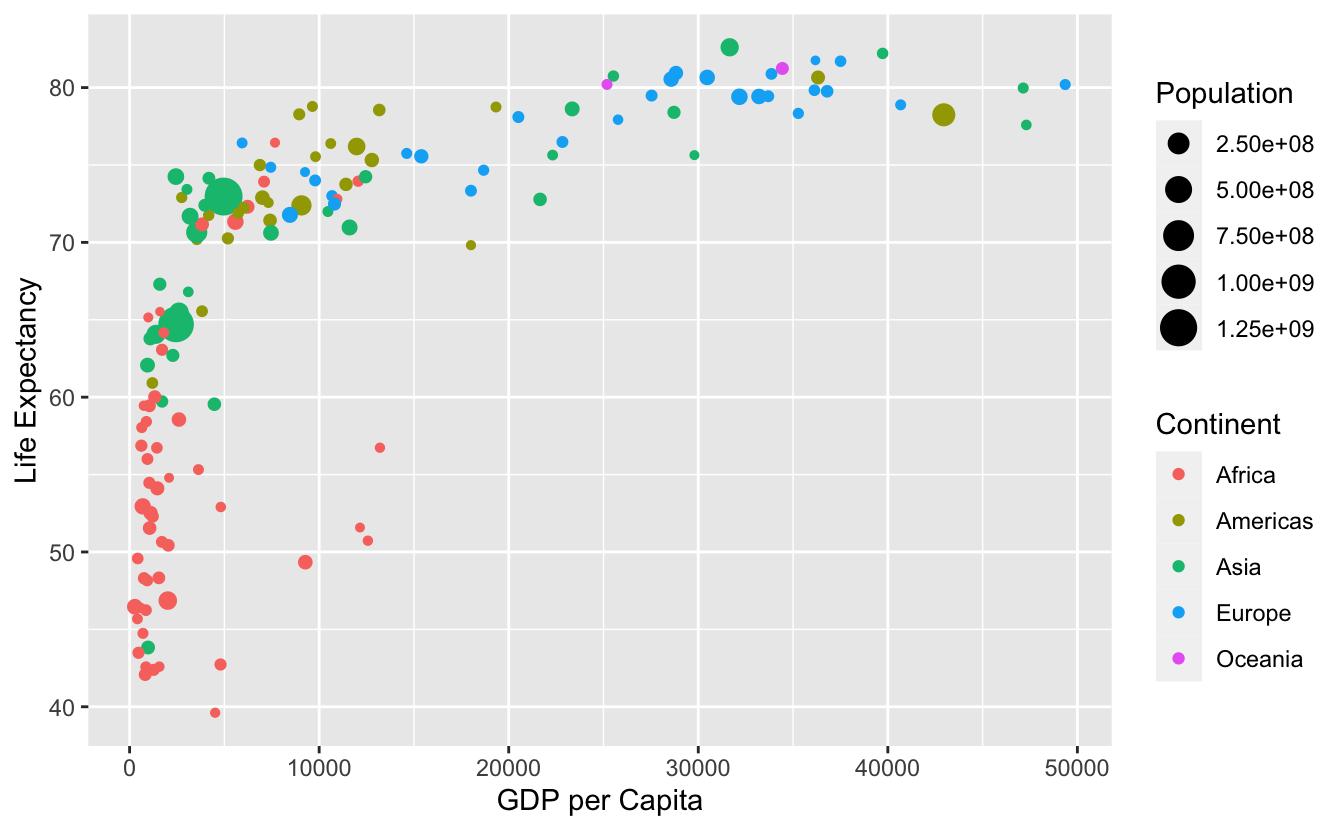
\includegraphics[width=0.9\linewidth]{figure/gapmind-1} 

}

\caption{Espérance de vie en fonction du PIB par habitant en 2007.}\label{fig:gapmind}
\end{figure}

Si on décrypte ce graphique du point de vue de la grammaire des graphiques, on voit que :

\begin{itemize}
\tightlist
\item
  la variable \texttt{GDP\ per\ Capita} est associée à l'\texttt{aes}thetic \texttt{x} de la position des points
\item
  la variable \texttt{Life\ Expectancy} est associée à l'\texttt{aes}thetic \texttt{y} de la position des points
\item
  la variable \texttt{Population} est associée à l'\texttt{aes}thetic \texttt{size} (taille) des points
\item
  la variable \texttt{Continent} est associée à l'\texttt{aes}thetic \texttt{color} (couleur) des points
\end{itemize}

Ici, l'objet géométrique (ou \texttt{geom}) qui représente les données est le point. Les données (ou \texttt{data}) sont contenues dans le tableau \texttt{gapminder} et chacune de ces variables est associée (\texttt{mapping}) aux caractéristiques esthétiques des points.

\hypertarget{autres-uxe9luxe9ments-de-la-grammaire-des-graphiques}{%
\subsubsection{Autres éléments de la grammaire des graphiques}\label{autres-uxe9luxe9ments-de-la-grammaire-des-graphiques}}

Outre les éléments indispensables évoqués ici (\texttt{data}, \texttt{mapping}, \texttt{aes}, et \texttt{geom}), il existe d'autres aspects de la grammaire des graphiques qui permettent de contrôler l'aspect des graphiques. Ils ne sont pas toujours indispensables. Nous en verrons néanmoins quelque-uns particulièrement utiles :

\begin{itemize}
\tightlist
\item
  \texttt{facet} : c'est un moyen très pratique de scinder le jeu de données en plusieurs sous-groupes et de produire automatiquement un graphique pour chacun d'entre eux.
\item
  \texttt{position} : permet notamment de modifier la position des barres d'un barplot.
\item
  \texttt{labs} : permet de définir les titres, sous-titres et légendes des axes d'un graphique
\item
  \texttt{theme} : permet de modifier l'apect général des graphiques en appliquant des thèmes prédéfinis ou en modifiant certains aspects de thèmes existants
\end{itemize}

\hypertarget{le-package-ggplot2}{%
\subsubsection{\texorpdfstring{Le package \texttt{ggplot2}}{Le package ggplot2}}\label{le-package-ggplot2}}

Comme indiqué plus haut, le package \texttt{ggplot2} (Wickham et al., \protect\hyperlink{ref-R-ggplot2}{2020}) permet de réaliser des graphiques dans R en respectant les principes de la grammaire des graphiques. Vous avez probablement remarqué que depuis le début de la section \ref{gggraph}, beaucoup de termes sont écrits dans la police réservée au \texttt{code} informatique. C'est parce que les éléments de la grammaire des graphiques sont tous précisés dans la fonction \texttt{ggplot()} qui demande, au grand minimum, que les éléments suivants soient spécifiés :

\begin{itemize}
\tightlist
\item
  le nom du \texttt{data.frame} contenant les variables qui seront utilisées pour le graphique. Ce nom correspond à l'argument \texttt{data} de la fonction \texttt{ggplot()}.
\item
  l'association des variables à des attributs esthétiques. Cela se fait grâce à l'argument \texttt{mapping} et la fonction \texttt{aes()}
\end{itemize}

Après avoir spécifié ces éléments, on ajoute des couches supplémentaires au graphique grâce au signe \texttt{+}. La couche la plus essentielle à ajouter à un graphique, est une couche contenant un élément géométrique, ou \texttt{geom} (par exemple des points, des lignes ou des barres). D'autres couches peuvent s'ajouter pour spécifier des titres, des \texttt{facet}s ou des modifications des axes et des thèmes du graphique.

Dans le cadre de ce cours, nous nous limiterons aux 5 types de graphiques suivants :

\begin{enumerate}
\def\labelenumi{\arabic{enumi}.}
\tightlist
\item
  les nuages de points
\item
  les graphiques en lignes
\item
  les boîtes à moustaches ou boxplots
\item
  les histogrammes
\item
  les diagrammes bâtons
\end{enumerate}

\begin{center}\rule{0.5\linewidth}{0.5pt}\end{center}

\hypertarget{clouds}{%
\subsection{Les nuages de points}\label{clouds}}

C'est probablement le plus simple des 5 types de graphiques cités plus haut. Il s'agit de graphiques bi-variés pour lesquels une variable est associée à l'axe des abscisses, et une autre est associée à l'axe des ordonnées. Comme pour le graphique présenté à la figure \ref{fig:gapmind} ci-dessus, d'autres variables peuvent être associées à des caractéristiques esthétiques des points (transparence, taille, couleur, forme\ldots).

Ici, dans le jeu de données \texttt{flights}, nous allons nous intéresser à la relation qui existe entre :

\begin{enumerate}
\def\labelenumi{\arabic{enumi}.}
\tightlist
\item
  \texttt{dep\_delay} : le retard des vols au décollage, que nous placerons sur l'axe des ``x''
\item
  \texttt{arr\_delay} : le retard des mêmes vols à l'atterrissage, que nous placerons sur l'axe des ``y''
\end{enumerate}

Afin d'avoir un jeu de données plus facile à utiliser, nous nous contenterons de visualiser les vols d'Alaska Airlines, dont le code de compagnie aérienne est \texttt{"AS"}.

\begin{Shaded}
\begin{Highlighting}[]
\NormalTok{alaska_flights <-}\StringTok{ }\NormalTok{flights }\OperatorTok
\StringTok{  }\KeywordTok{filter}\NormalTok{(carrier }\OperatorTok{==}\StringTok{ "AS"}\NormalTok{)}
\end{Highlighting}
\end{Shaded}

Il est normal que vous ne compreniez pas encore les commandes ci-dessus : elles seront décrites dans le chapitre \ref{wrangling}. Retenez juste que nous avons créé un nouveau tableau, nommé \texttt{alaska\_flights}, qui contient toutes les informations des vols d'Alaska Airlines. Commencez par examiner ce tableau avec la fonction \texttt{View()}. En quoi est-il différent du tableau \texttt{flights} ?

\hypertarget{la-couche-de-base-la-fonction-ggplot}{%
\subsubsection{\texorpdfstring{La couche de base : la fonction \texttt{ggplot()}}{La couche de base : la fonction ggplot()}}\label{la-couche-de-base-la-fonction-ggplot}}

La fonction \texttt{ggplot()} permet d'établir la première base du graphique. C'est grâce à cette fonction que l'on précise quel jeu de données utiliser et quelles variables placer sur les axes :

\begin{Shaded}
\begin{Highlighting}[]
\KeywordTok{ggplot}\NormalTok{(}\DataTypeTok{data =}\NormalTok{ alaska_flights, }\DataTypeTok{mapping =} \KeywordTok{aes}\NormalTok{(}\DataTypeTok{x =}\NormalTok{ dep_delay, }\DataTypeTok{y =}\NormalTok{ arr_delay))}
\end{Highlighting}
\end{Shaded}

\begin{figure}[htpb]

{\centering 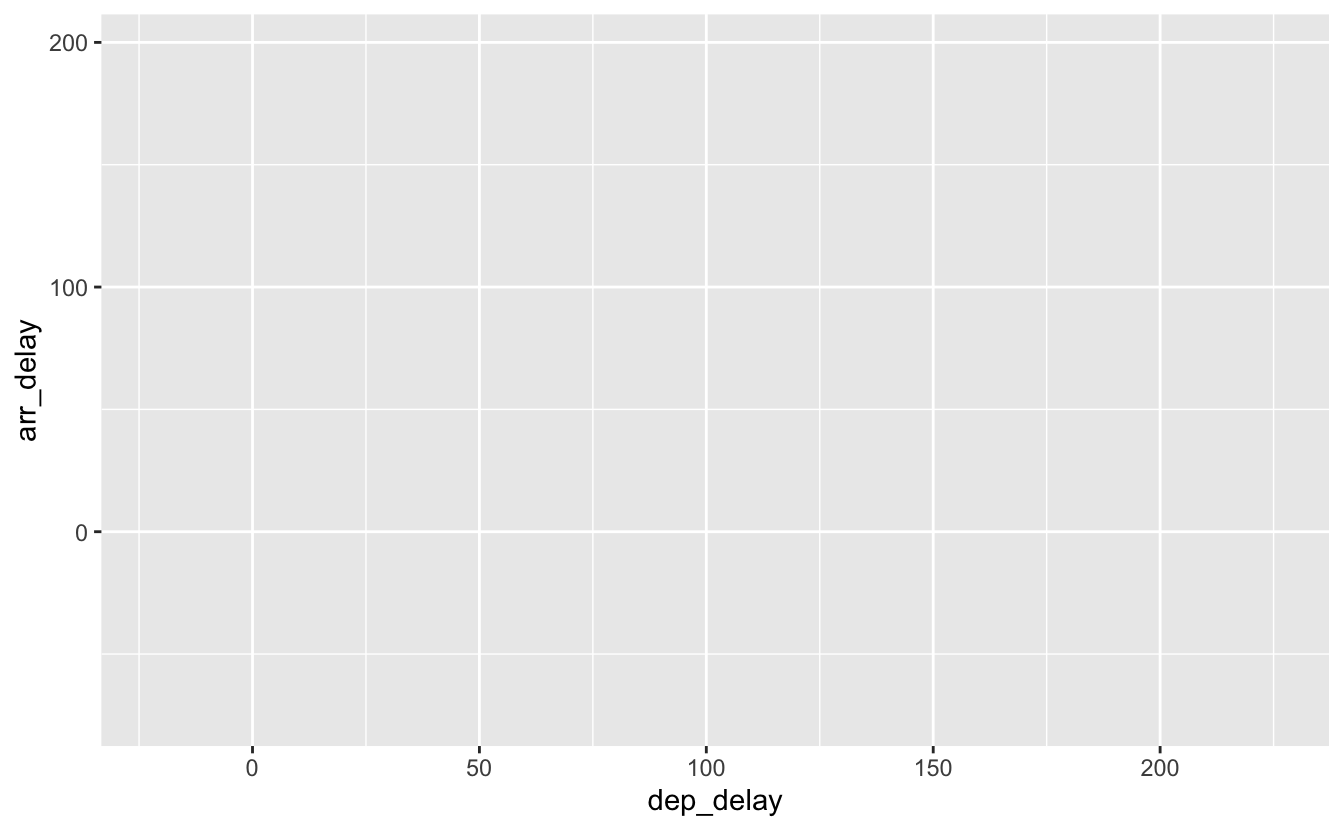
\includegraphics[width=0.9\linewidth]{figure/unnamed-chunk-40-1} 

}

\caption{Un graphique sans `geom`.}\label{fig:unnamed-chunk-40}
\end{figure}

Ce graphique est pour le moins vide : c'est normal, nous n'avons pas encore spécifié la couche contenant l'objet géométrique que nous souhaitons utiliser.

\hypertarget{ajout-dune-couche-suppluxe9mentaire-lobjet-guxe9omuxe9trique}{%
\subsubsection{Ajout d'une couche supplémentaire : l'objet géométrique}\label{ajout-dune-couche-suppluxe9mentaire-lobjet-guxe9omuxe9trique}}

Les nuages de points sont créés par la fonction \texttt{geom\_point()} :

\begin{Shaded}
\begin{Highlighting}[]
\KeywordTok{ggplot}\NormalTok{(}\DataTypeTok{data =}\NormalTok{ alaska_flights, }\DataTypeTok{mapping =} \KeywordTok{aes}\NormalTok{(}\DataTypeTok{x =}\NormalTok{ dep_delay, }\DataTypeTok{y =}\NormalTok{ arr_delay)) }\OperatorTok{+}\StringTok{ }
\StringTok{  }\KeywordTok{geom_point}\NormalTok{()}
\end{Highlighting}
\end{Shaded}

\begin{verbatim}
Warning: Removed 5 rows containing missing values (geom_point).
\end{verbatim}

\begin{figure}[!htpb]

{\centering 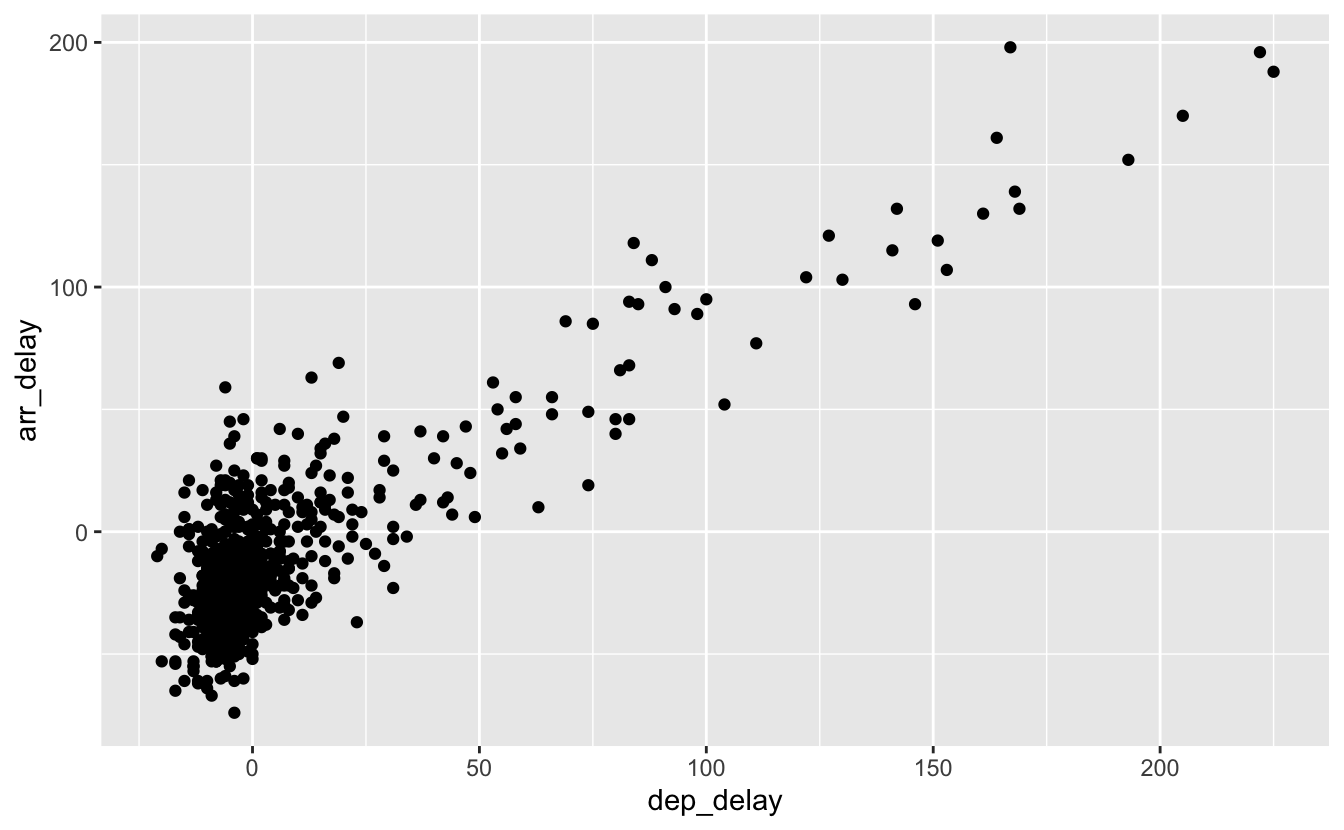
\includegraphics[width=0.9\linewidth]{figure/points-1} 

}

\caption{Retards à l'arrivée en fonction des retards au décollage pour les vols d'Alaska Airlines au départ de New York City en 2013.}\label{fig:points}
\end{figure}

Plusieurs choses importantes sont à remarquer sur la figure \ref{fig:points} :

\begin{enumerate}
\def\labelenumi{\arabic{enumi}.}
\tightlist
\item
  le graphique présente maintenant une couche supplémentaire constituée de points.
\item
  la fonction \texttt{geom\_point()} nous prévient que 5 lignes contenant des données manquantes n'ont pas été intégrées au graphique. Les données manquent soit pour une variable, soit pour l'autre, soit pour les 2. Il est donc impossible de les faire apparaître sur le graphique.
\item
  il existe une relation positive entre \texttt{dep\_delay} et \texttt{arr\_delay} : quand le retard d'un vol au décollage augmente, le retard de ce vol augmente aussi à l'arrivée.
\item
  Enfin, il y a une grande majorité de points centrés près de l'origine (0,0).
\end{enumerate}

Si je résume cette syntaxe :

\begin{itemize}
\tightlist
\item
  Au sein de la fonction \texttt{ggplot()}, on spécifie 2 composants de la grammaire des graphiques :

  \begin{enumerate}
  \def\labelenumi{\arabic{enumi}.}
  \tightlist
  \item
    le nom du tableau contenant les données grâce à l'argument \texttt{data\ =\ alaska\_flights}
  \item
    l'association (\texttt{mapping}) des variables à des caractéristiques esthétiques (\texttt{aes()}) en précisant \texttt{aes(x\ =\ dep\_delay,\ y\ =\ arr\_delay)} :

    \begin{itemize}
    \tightlist
    \item
      la variable \texttt{dep\_delay} est associée à l'esthétique de position \texttt{x}
    \item
      la variable \texttt{arr\_delay} est associée à l'esthétique de position \texttt{y}
    \end{itemize}
  \end{enumerate}
\item
  On ajoute une couche au graphique \texttt{ggplot()} grâce au symbole \texttt{+}. La couche en question précise le troisème élément indispensable de la grammaire des graphiques : l'objet \texttt{geom}étrique. Ici, les objets sont des \texttt{point}s. On le spécifie grâce à la fonction \texttt{geom\_point()}.
\end{itemize}

Quelques remarques concernant les couches :

\begin{itemize}
\tightlist
\item
  Notez que le signe \texttt{+} est placé \emph{à la fin de la ligne}. Vous recevrez un message d'erreur si vous le placez au début.
\item
  Quand vous ajoutez une couche à un graphique, je vous encourage vivement à presser la touche \texttt{enter} de votre clavier juste après le symbole \texttt{+}. Ainsi, le code correspondant à chaque couche sera sur une ligne distincte, ce qui augmente considérablement la lisibilité de votre code.
\item
  Comme indiqué dans la section \ref{functions}, tant que les arguments d'une fonction sont spécifiés dans l'ordre, on peut se passer d'écrire leur nom. Ainsi, les deux blocs de commande suivants produisent exactement le même résultat :
\end{itemize}

\begin{Shaded}
\begin{Highlighting}[]
\CommentTok{# Le nom des arguments est précisé}
\KeywordTok{ggplot}\NormalTok{(}\DataTypeTok{data =}\NormalTok{ alaska_flights, }\DataTypeTok{mapping =} \KeywordTok{aes}\NormalTok{(}\DataTypeTok{x =}\NormalTok{ dep_delay, }\DataTypeTok{y =}\NormalTok{ arr_delay)) }\OperatorTok{+}\StringTok{ }
\StringTok{  }\KeywordTok{geom_point}\NormalTok{()}

\CommentTok{# Le nom des arguments est omis}
\KeywordTok{ggplot}\NormalTok{(alaska_flights, }\KeywordTok{aes}\NormalTok{(}\DataTypeTok{x =}\NormalTok{ dep_delay, }\DataTypeTok{y =}\NormalTok{ arr_delay)) }\OperatorTok{+}\StringTok{ }
\StringTok{  }\KeywordTok{geom_point}\NormalTok{()}
\end{Highlighting}
\end{Shaded}

\hypertarget{exercices-2}{%
\subsubsection{Exercices}\label{exercices-2}}

\begin{enumerate}
\def\labelenumi{\arabic{enumi}.}
\tightlist
\item
  Donnez une raison pratique expliquant pourquoi les variables \texttt{dep\_delay} et \texttt{arr\_delay} ont une relation positive
\item
  Quelles variables (pas nécessairement dans le tableau \texttt{alaska\_flights}) pourraient avoir une corrélation négative (relation négative) avec \texttt{dep\_delay} ? Pourquoi ? Rappelez-vous que nous étudions ici des variables numériques.
\item
  Selon vous, pourquoi tant de points sont-il regroupés près de (0, 0) ? À quoi le point (0,0) correspond-il pour les vols d'Alaska Airlines ?
\item
  Citez les éléments de ce graphique/de ces données qui vous sautent le plus aux yeux ?
\item
  Créez un nouveau nuage de points en utilisant d'autres variables du jeu de données \texttt{alaska\_flights}
\end{enumerate}

\hypertarget{over-plotting}{%
\subsubsection{Over-plotting}\label{over-plotting}}

L'over-plotting est la superposition importante d'une grande quantité d'information sur une zone restreinte d'un graphique. Dans notre cas, nous observons un over-plotting important autour de (0,0). Cet effet est gênant car il est difficile de se faire une idée précise du nombre de points accumulés dans cette zone. La façon la plus simple de régler le problème est de modifier la transparence des points grâce à l'argument \texttt{alpha} de la fonction \texttt{geom\_point()}. Par défaut, cette valeur est fixée à 1, pour une opacité totale. Une valeur de 0 rend les points totalement transparents, et donc invisibles. Trouver la bonne valeur peut demander de tâtonner un peu. Le code suivant produit la figure \ref{fig:transparent} :

\begin{Shaded}
\begin{Highlighting}[]
\KeywordTok{ggplot}\NormalTok{(}\DataTypeTok{data =}\NormalTok{ alaska_flights, }
       \DataTypeTok{mapping =} \KeywordTok{aes}\NormalTok{(}\DataTypeTok{x =}\NormalTok{ dep_delay, }\DataTypeTok{y =}\NormalTok{ arr_delay)) }\OperatorTok{+}\StringTok{ }
\StringTok{  }\KeywordTok{geom_point}\NormalTok{(}\DataTypeTok{alpha =} \FloatTok{0.2}\NormalTok{)}
\end{Highlighting}
\end{Shaded}

\begin{figure}[htpb]

{\centering 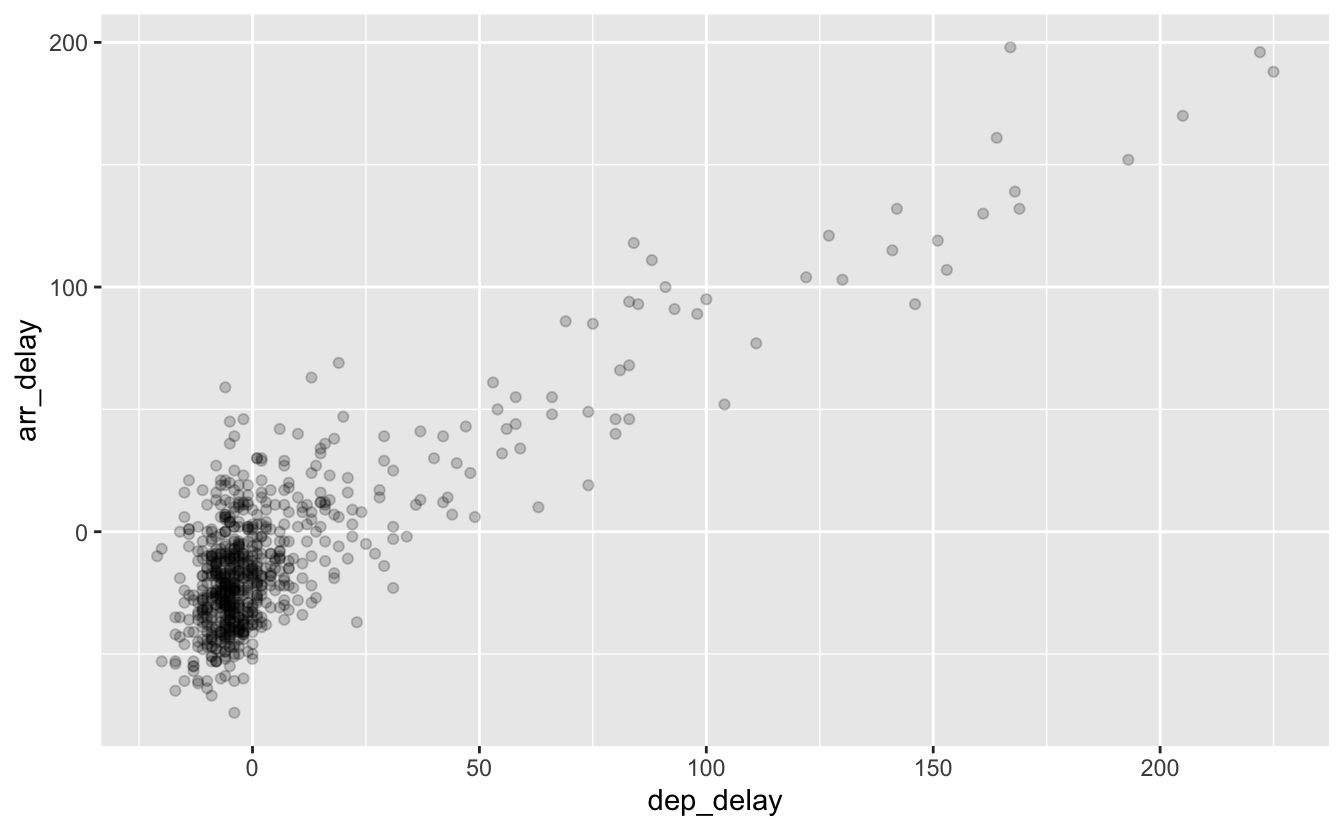
\includegraphics[width=0.9\linewidth]{figure/transparent-1} 

}

\caption{La même figure, avec des points semi-transparents.}\label{fig:transparent}
\end{figure}

Sur cette figure, notez que :

\begin{itemize}
\tightlist
\item
  la transparence est additive : plus il y a de points, plus la zone est foncée car les points se superposent et rendent la zone plus opaque.
\item
  l'argument \texttt{alpha\ =} n'est pas intégré à l'intérieur d'une fonction \texttt{aes()} car ici, il n'est pas associé à une variable : c'est un simple paramètre.
\end{itemize}

L'over-plotting est souvent rencontré lorsque l'on représente plusieurs nuages de points pour les différentes valeurs d'une variable catégorielle. Par exemple, si on transforme la variable \texttt{month} en facteur (\texttt{factor(month)}), on peut regarder s'il existe une relation entre les retards à l'atterrissage et le mois de l'année :

\begin{Shaded}
\begin{Highlighting}[]
\KeywordTok{ggplot}\NormalTok{(}\DataTypeTok{data =}\NormalTok{ alaska_flights, }
       \DataTypeTok{mapping =} \KeywordTok{aes}\NormalTok{(}\DataTypeTok{x =} \KeywordTok{factor}\NormalTok{(month), }\DataTypeTok{y =}\NormalTok{ arr_delay)) }\OperatorTok{+}
\StringTok{  }\KeywordTok{geom_point}\NormalTok{()}
\end{Highlighting}
\end{Shaded}

\begin{figure}[htpb]

{\centering 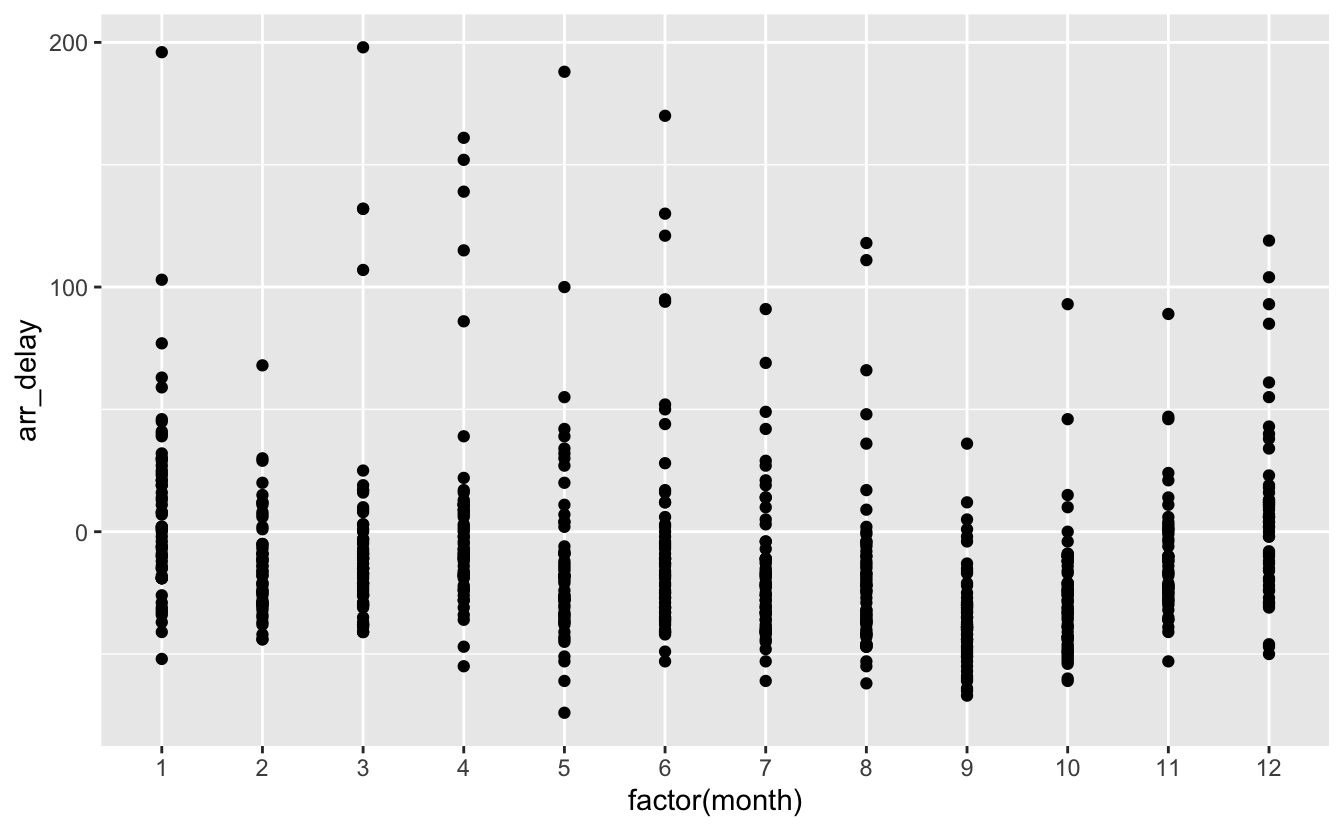
\includegraphics[width=0.9\linewidth]{figure/transpfactor-1} 

}

\caption{Retards à l'arrivée pour les 12 mois de l'année 2013.}\label{fig:transpfactor}
\end{figure}

Ici (figure \ref{fig:transpfactor}), l'ajout de transparence ne serait pas suffisant. Une autre solution est d'appliquer la méthode dîte du ``jittering'', ou tremblement. Elle consiste à ajouter un bruit aléatoire horizontal et/ou vertical aux points d'un graphique. Ici, on peut ajouter un léger bruit horizontal afin de disperser un peu les points pour chaque mois de l'année. On n'ajoute pas de bruit vertical car on ne souhaite pas que les valeurs de retard (sur l'axe des \texttt{y}) soient altérées :

\begin{Shaded}
\begin{Highlighting}[]
\KeywordTok{ggplot}\NormalTok{(}\DataTypeTok{data =}\NormalTok{ alaska_flights, }
       \DataTypeTok{mapping =} \KeywordTok{aes}\NormalTok{(}\DataTypeTok{x =} \KeywordTok{factor}\NormalTok{(month), }\DataTypeTok{y =}\NormalTok{ arr_delay)) }\OperatorTok{+}
\StringTok{  }\KeywordTok{geom_jitter}\NormalTok{(}\DataTypeTok{width =} \FloatTok{0.25}\NormalTok{)}
\end{Highlighting}
\end{Shaded}

\begin{figure}[htpb]

{\centering 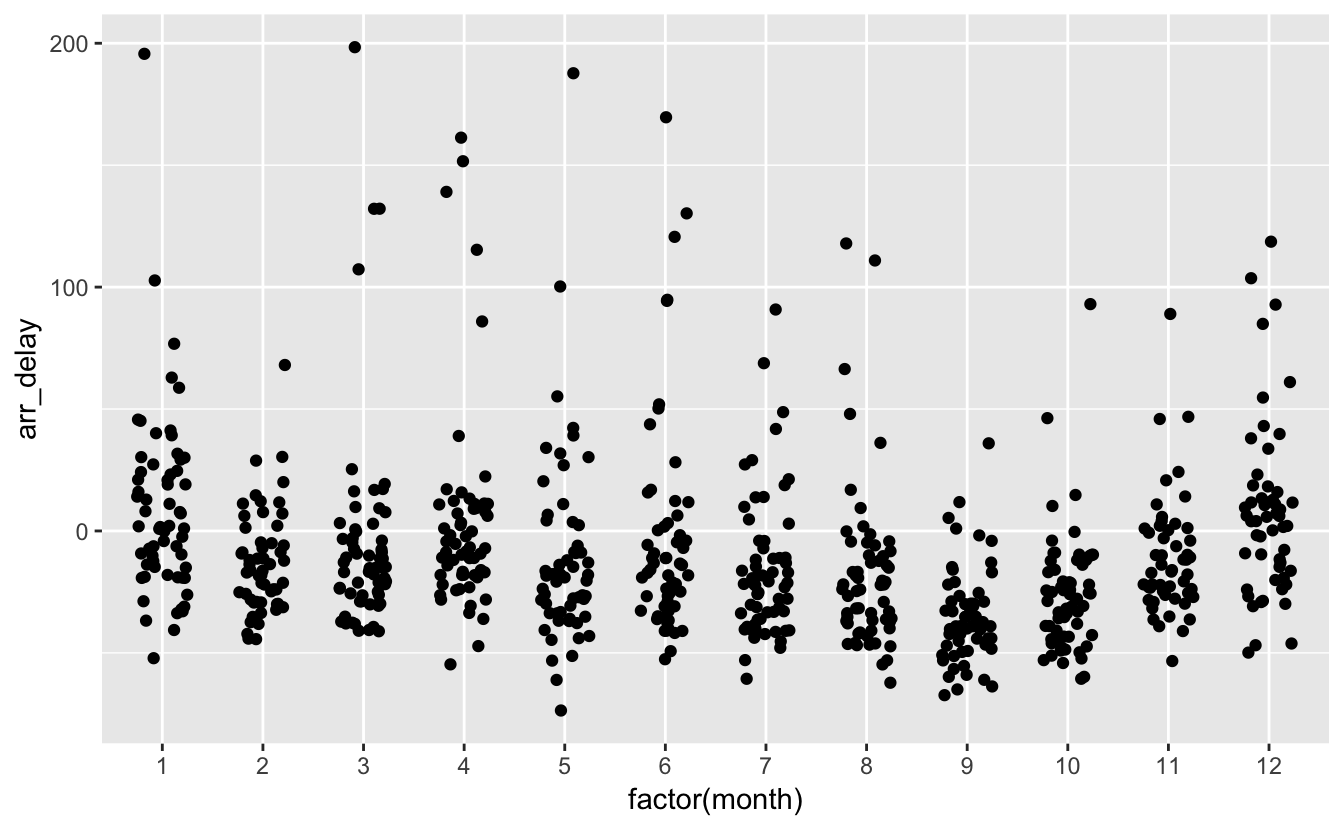
\includegraphics[width=0.9\linewidth]{figure/jittering-1} 

}

\caption{Retards à l'arrivée pour les 12 mois de l'année 2013.}\label{fig:jittering}
\end{figure}

On y voit déjà plus clair. L'argument \texttt{width} permet de spécifier l'intensité de la dispersion horizontale. Pour ajouter du bruit vertical (ce qui n'est pas souhaitable ici !), on peut ajouter l'argument \texttt{height}. Le graphique de la figure \ref{fig:jittering} est parfois appelé un ``stripchart''. C'est un graphique du type ``nuage de points'', mais pour lequel l'une des 2 variables est numérique, et l'autre est catégorielle.

Il est évidemment possible d'ajouter de la transparence :

\begin{Shaded}
\begin{Highlighting}[]
\KeywordTok{ggplot}\NormalTok{(}\DataTypeTok{data =}\NormalTok{ alaska_flights, }
       \DataTypeTok{mapping =} \KeywordTok{aes}\NormalTok{(}\DataTypeTok{x =} \KeywordTok{factor}\NormalTok{(month), }\DataTypeTok{y =}\NormalTok{ arr_delay)) }\OperatorTok{+}
\StringTok{  }\KeywordTok{geom_jitter}\NormalTok{(}\DataTypeTok{width =} \FloatTok{0.25}\NormalTok{, }\DataTypeTok{alpha =} \FloatTok{0.5}\NormalTok{)}
\end{Highlighting}
\end{Shaded}

\begin{figure}[htpb]

{\centering 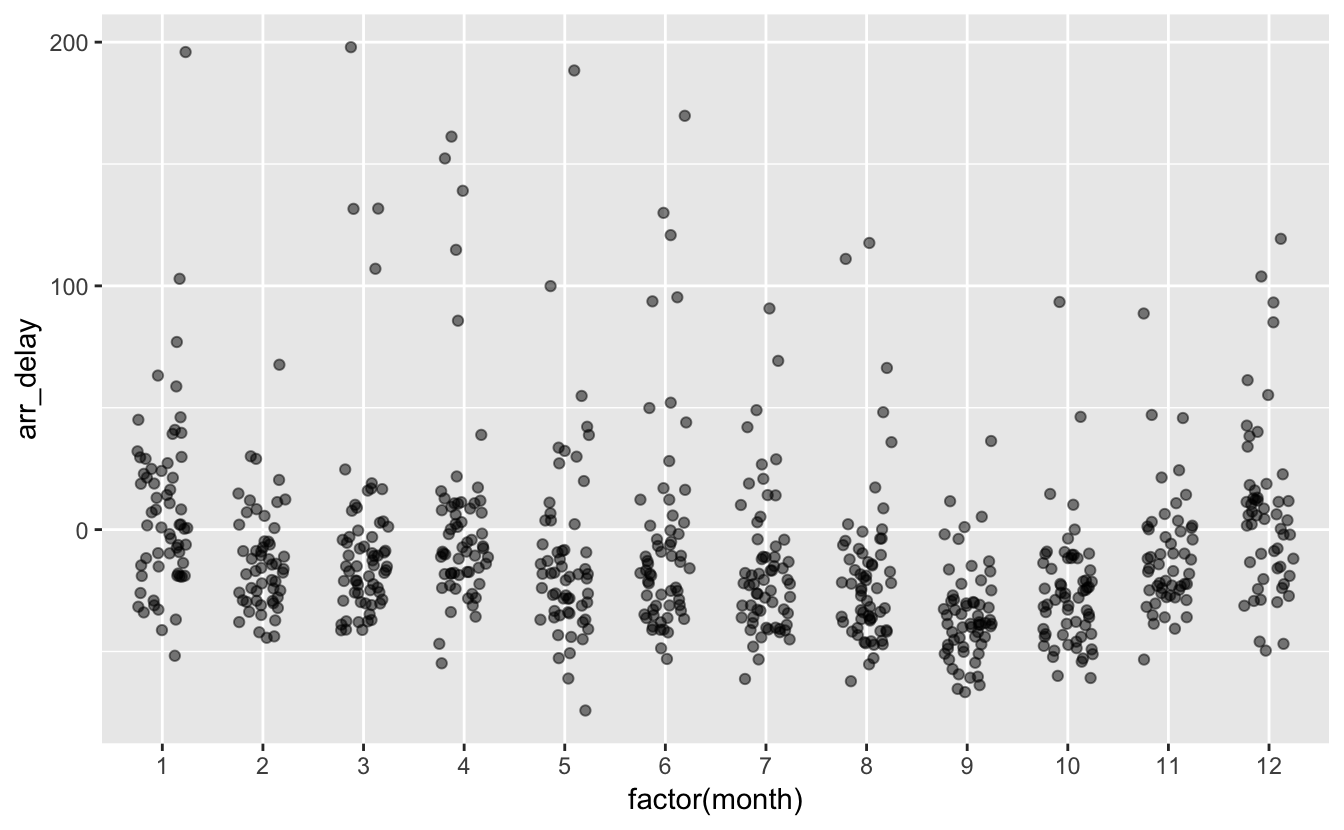
\includegraphics[width=0.9\linewidth]{figure/unnamed-chunk-42-1} 

}

\caption{Retards à l'arrivée pour les 12 mois de l'année 2013.}\label{fig:unnamed-chunk-42}
\end{figure}

\hypertarget{couleur-taille-et-forme}{%
\subsubsection{Couleur, taille et forme}\label{couleur-taille-et-forme}}

L'argument \texttt{color} (ou \texttt{colour}, les deux orthographes fonctionnent) permet de spécifier la couleur des points. L'argument \texttt{size} permet de spécifier la taille des points. L'argument \texttt{shape} permet de spécifier la forme utilisée en guise de symbole. Ces 3 arguments peuvent être utilisés comme des paramètres, pour modifier l'ensemble des points d'un graphique. Mais ils peuvent aussi être associés à une variable, pour apporter une information supplémentaire.

Comparez les deux graphiques suivants (figures \ref{fig:rightcolor} et \ref{fig:wrongcolor}) :

\begin{Shaded}
\begin{Highlighting}[]
\KeywordTok{ggplot}\NormalTok{(}\DataTypeTok{data =}\NormalTok{ alaska_flights, }\DataTypeTok{mapping =} \KeywordTok{aes}\NormalTok{(}\DataTypeTok{x =}\NormalTok{ dep_delay, }\DataTypeTok{y =}\NormalTok{ arr_delay)) }\OperatorTok{+}
\StringTok{  }\KeywordTok{geom_point}\NormalTok{(}\DataTypeTok{color =} \StringTok{"blue"}\NormalTok{)}
\end{Highlighting}
\end{Shaded}

\begin{figure}[htpb]

{\centering 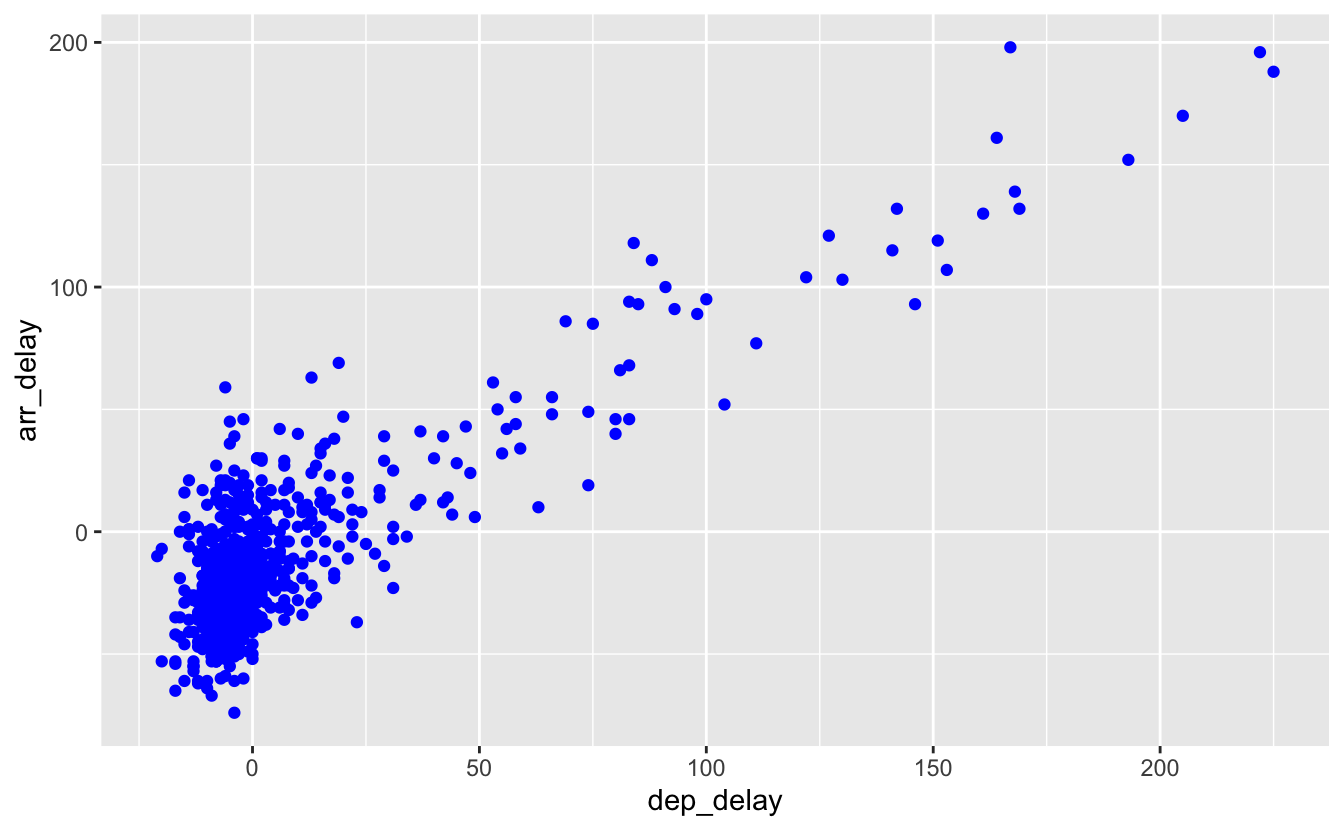
\includegraphics[width=0.9\linewidth]{figure/rightcolor-1} 

}

\caption{Utilisation correcte de `color`.}\label{fig:rightcolor}
\end{figure}

\begin{Shaded}
\begin{Highlighting}[]
\KeywordTok{ggplot}\NormalTok{(}\DataTypeTok{data =}\NormalTok{ alaska_flights, }\DataTypeTok{mapping =} \KeywordTok{aes}\NormalTok{(}\DataTypeTok{x =}\NormalTok{ dep_delay, }\DataTypeTok{y =}\NormalTok{ arr_delay)) }\OperatorTok{+}
\StringTok{  }\KeywordTok{geom_point}\NormalTok{(}\KeywordTok{aes}\NormalTok{(}\DataTypeTok{color =} \StringTok{"blue"}\NormalTok{))}
\end{Highlighting}
\end{Shaded}

\begin{figure}[htpb]

{\centering 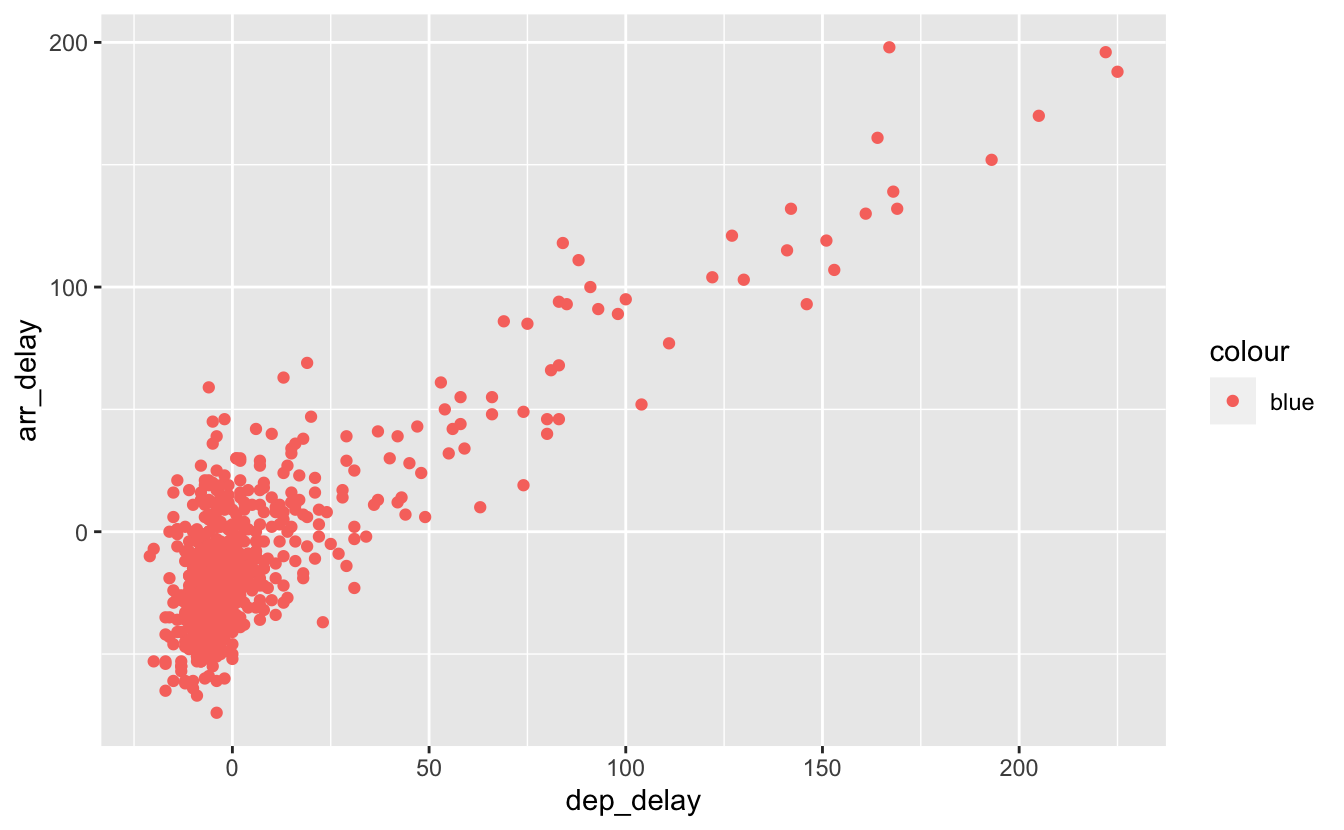
\includegraphics[width=0.9\linewidth]{figure/wrongcolor-1} 

}

\caption{Utilisation incorrecte de `color`.}\label{fig:wrongcolor}
\end{figure}

Le code qui permet de produire la figure \ref{fig:rightcolor} fait un usage correct de l'argument \texttt{color}. On demande des points de couleur bleue, les points apparaîssent bleus. La figure \ref{fig:wrongcolor} en revanche ne produit pas le résultat attendu. Puisque nous avons mis l'argument \texttt{color} à l'intérieur de la fonction \texttt{aes()}, R s'attend à ce que la couleur soit associée à une variable. Puisqu'aucune variable ne s'appelle ``blue'', R utilise la couleur par défaut. Pour associer la couleur des points à une variable, nous devons fournir un nom de variable valide :

\begin{Shaded}
\begin{Highlighting}[]
\KeywordTok{ggplot}\NormalTok{(}\DataTypeTok{data =}\NormalTok{ alaska_flights, }\DataTypeTok{mapping =} \KeywordTok{aes}\NormalTok{(}\DataTypeTok{x =}\NormalTok{ dep_delay, }\DataTypeTok{y =}\NormalTok{ arr_delay)) }\OperatorTok{+}
\StringTok{  }\KeywordTok{geom_point}\NormalTok{(}\KeywordTok{aes}\NormalTok{(}\DataTypeTok{color =} \KeywordTok{factor}\NormalTok{(month)))}
\end{Highlighting}
\end{Shaded}

\begin{figure}[htpb]

{\centering 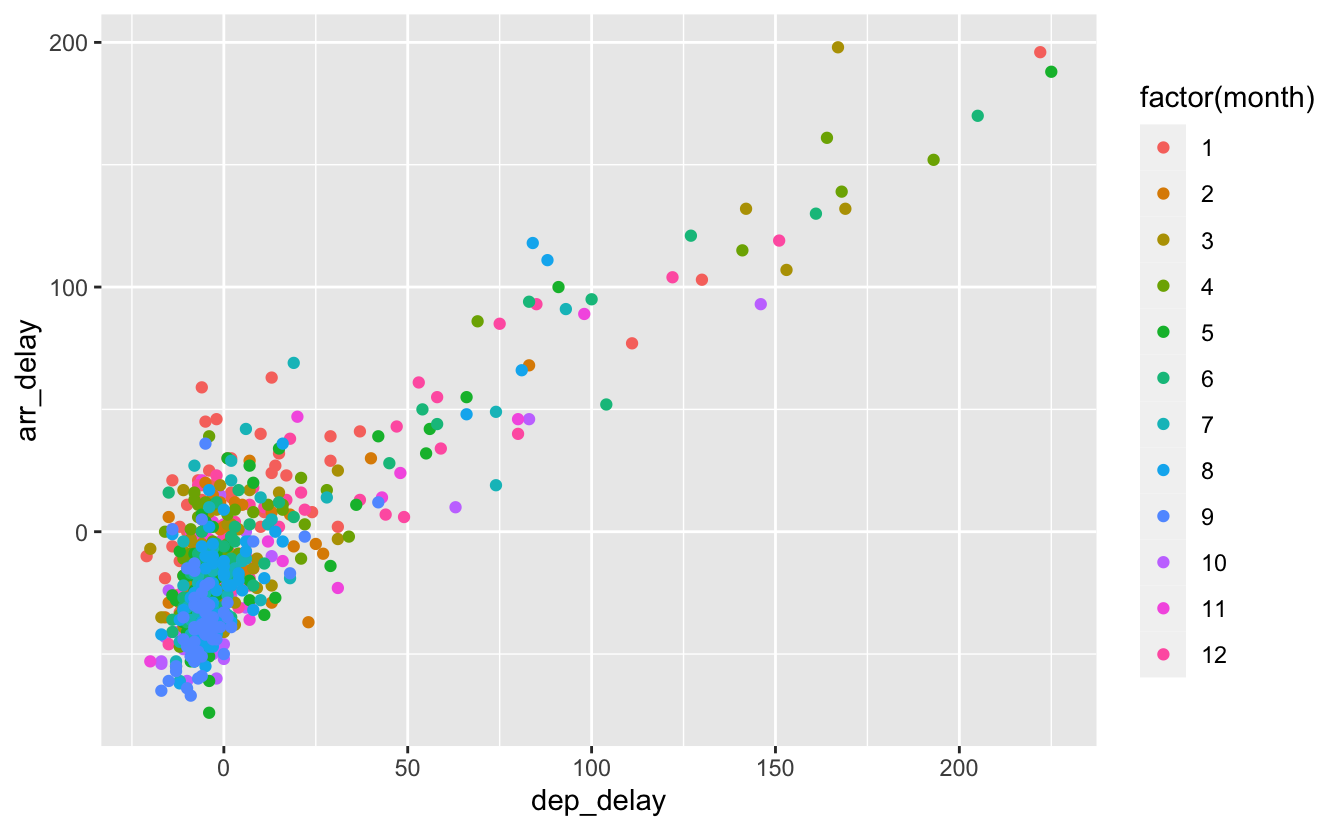
\includegraphics[width=0.9\linewidth]{figure/varcolor-1} 

}

\caption{Association de `color` à une variable catégorielle.}\label{fig:varcolor}
\end{figure}

Ici, l'utilisation de la couleur est correcte. Elle est associée à une variable catégorielle, et chaque valeur possible du vecteur \texttt{month} se voit donc attribuer une couleur différente.

\begin{Shaded}
\begin{Highlighting}[]
\KeywordTok{ggplot}\NormalTok{(}\DataTypeTok{data =}\NormalTok{ alaska_flights, }\DataTypeTok{mapping =} \KeywordTok{aes}\NormalTok{(}\DataTypeTok{x =}\NormalTok{ dep_delay, }\DataTypeTok{y =}\NormalTok{ arr_delay)) }\OperatorTok{+}
\StringTok{  }\KeywordTok{geom_point}\NormalTok{(}\KeywordTok{aes}\NormalTok{(}\DataTypeTok{color =}\NormalTok{ arr_time))}
\end{Highlighting}
\end{Shaded}

\begin{figure}[htpb]

{\centering 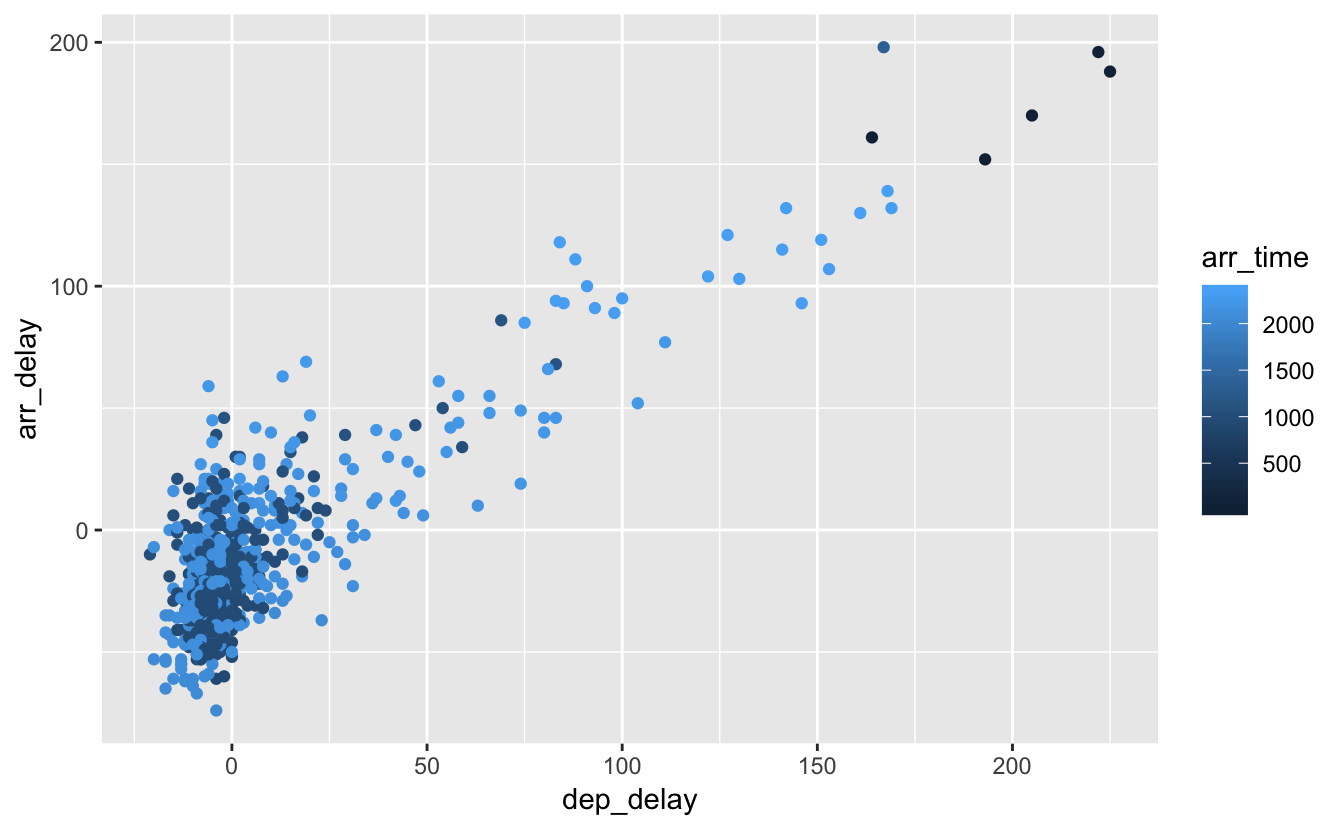
\includegraphics[width=0.9\linewidth]{figure/varcolor2-1} 

}

\caption{Association de `color` à une variable numérique.}\label{fig:varcolor2}
\end{figure}

De la même façon, la couleur des points est ici associée à une variable continue (l'heure d'arrivée des vols). Les points se voient donc attribuer une couleur choisie le long d'un gradient.

La même approche peut être utilisée pour spécifier la forme des symboles avec l'argument \texttt{shape}. Attention toutefois : une variable continue ne peut pas être associée à \texttt{shape}

\begin{Shaded}
\begin{Highlighting}[]
\KeywordTok{ggplot}\NormalTok{(}\DataTypeTok{data =}\NormalTok{ alaska_flights, }\DataTypeTok{mapping =} \KeywordTok{aes}\NormalTok{(}\DataTypeTok{x =}\NormalTok{ dep_delay, }\DataTypeTok{y =}\NormalTok{ arr_delay)) }\OperatorTok{+}
\StringTok{  }\KeywordTok{geom_point}\NormalTok{(}\KeywordTok{aes}\NormalTok{(}\DataTypeTok{shape =} \KeywordTok{factor}\NormalTok{(month)))}
\end{Highlighting}
\end{Shaded}

\begin{figure}[htpb]

{\centering 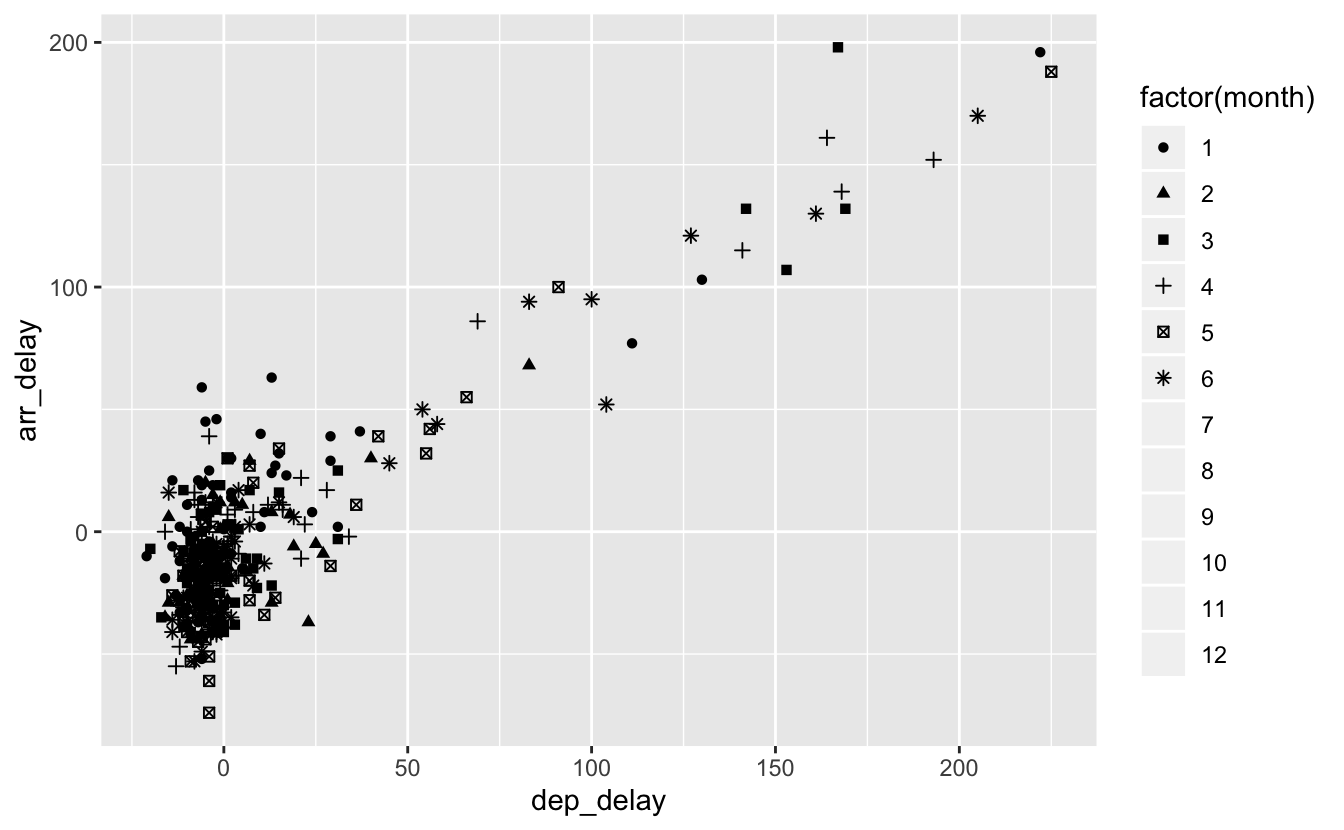
\includegraphics[width=0.9\linewidth]{figure/shapeplot-1} 

}

\caption{Association de `shape` à un facteur.}\label{fig:shapeplot}
\end{figure}

Vous noterez que seuls les 6 premiers niveaux d'un facteur se voient attribuer une forme automatiquement. Au delà de 6 symboles différents sur un même graphique, le résultat est souvent illisible. Il est possible d'ajouter plus de 6 symboles, mais cela demande de modifier la légende manuellement et concrètement nous n'en aurons jamais besoin. Lorsque plus de 6 séries doivent être distinguées, d'autres solutions bien plus pertinentes (par exemple les \texttt{factet}s) devraient être utilisées.

Comme pour la couleur, il est possible d'utiliser l'argument \texttt{shape} en tant que paramètre du graphique sans l'associer à une variable. Il faut alors fournir un code compris entre 0 et 24 :

\begin{Shaded}
\begin{Highlighting}[]
\KeywordTok{ggplot}\NormalTok{(}\DataTypeTok{data =}\NormalTok{ alaska_flights, }\DataTypeTok{mapping =} \KeywordTok{aes}\NormalTok{(}\DataTypeTok{x =}\NormalTok{ dep_delay, }\DataTypeTok{y =}\NormalTok{ arr_delay)) }\OperatorTok{+}
\StringTok{  }\KeywordTok{geom_point}\NormalTok{(}\DataTypeTok{shape =} \DecValTok{4}\NormalTok{)}
\end{Highlighting}
\end{Shaded}

\begin{figure}[htpb]

{\centering 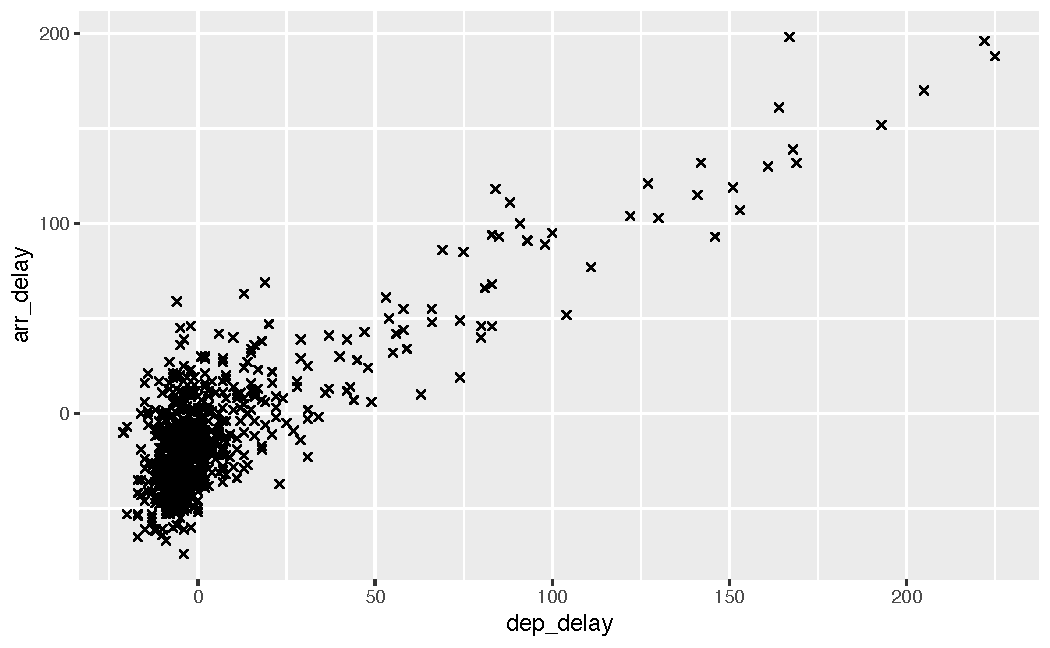
\includegraphics[width=0.9\linewidth]{figure/shapeplot2-1} 

}

\caption{Utilisation de `shape` en tant que paramètre.}\label{fig:shapeplot2}
\end{figure}

Notez qu'ici, \texttt{ggplot()} ne crée pas de légende : tous les points ont le même symbole, ce symbole n'est pas associé à une variable, une légende est donc inutile.

Parmi les valeurs possibles pour \texttt{shape}, les symboles 21 à 24 sont des symboles dont on peut spécifier séparément la couleur de contour, avec \texttt{color} et la couleur de fond avec \texttt{fill} :

\begin{Shaded}
\begin{Highlighting}[]
\KeywordTok{ggplot}\NormalTok{(}\DataTypeTok{data =}\NormalTok{ alaska_flights, }\DataTypeTok{mapping =} \KeywordTok{aes}\NormalTok{(}\DataTypeTok{x =}\NormalTok{ dep_delay, }\DataTypeTok{y =}\NormalTok{ arr_delay)) }\OperatorTok{+}
\StringTok{  }\KeywordTok{geom_point}\NormalTok{(}\DataTypeTok{shape =} \DecValTok{21}\NormalTok{, }\DataTypeTok{fill =} \StringTok{"steelblue"}\NormalTok{, }\DataTypeTok{color =} \StringTok{"orange"}\NormalTok{, }\DataTypeTok{alpha =} \FloatTok{0.5}\NormalTok{)}
\end{Highlighting}
\end{Shaded}

\begin{figure}[htpb]

{\centering 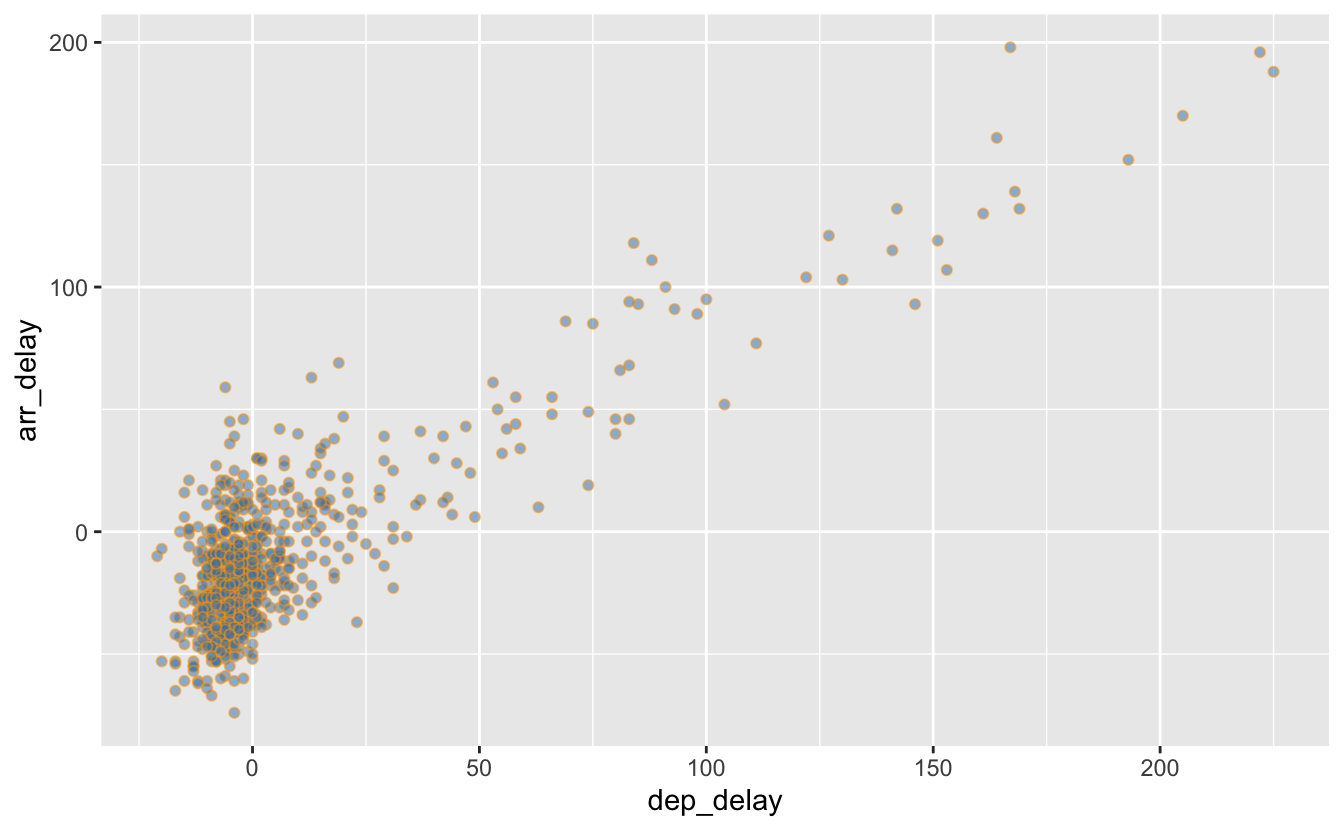
\includegraphics[width=0.9\linewidth]{figure/shapecolorplot-1} 

}

\caption{Utilisation de `shape`, `color` et `fill`.}\label{fig:shapecolorplot}
\end{figure}

N'hésitez pas à zoomer pour bien observer les points et comprendre ce qui se passe. Un conseil, faites des choix raisonnables ! Trop de couleurs n'est pas forcément souhaitable.

Enfin, on peut ajuster la taille des symboles avec l'argument \texttt{size}. Tout comme il n'est pas possible d'associer une variable continue à \texttt{shape}, il n'est pas conseillé d'associer une variable catégorielle nominale (c'est-à-dire un facteur non ordonné) à \texttt{size}. Associer une variable continue est en ravanche parfois utile :

\begin{Shaded}
\begin{Highlighting}[]
\KeywordTok{ggplot}\NormalTok{(}\DataTypeTok{data =}\NormalTok{ alaska_flights, }\DataTypeTok{mapping =} \KeywordTok{aes}\NormalTok{(}\DataTypeTok{x =}\NormalTok{ dep_delay, }\DataTypeTok{y =}\NormalTok{ arr_delay)) }\OperatorTok{+}
\StringTok{  }\KeywordTok{geom_point}\NormalTok{(}\KeywordTok{aes}\NormalTok{(}\DataTypeTok{size =}\NormalTok{ arr_time), }\DataTypeTok{alpha =} \FloatTok{0.1}\NormalTok{)}
\end{Highlighting}
\end{Shaded}

\begin{figure}[htpb]

{\centering 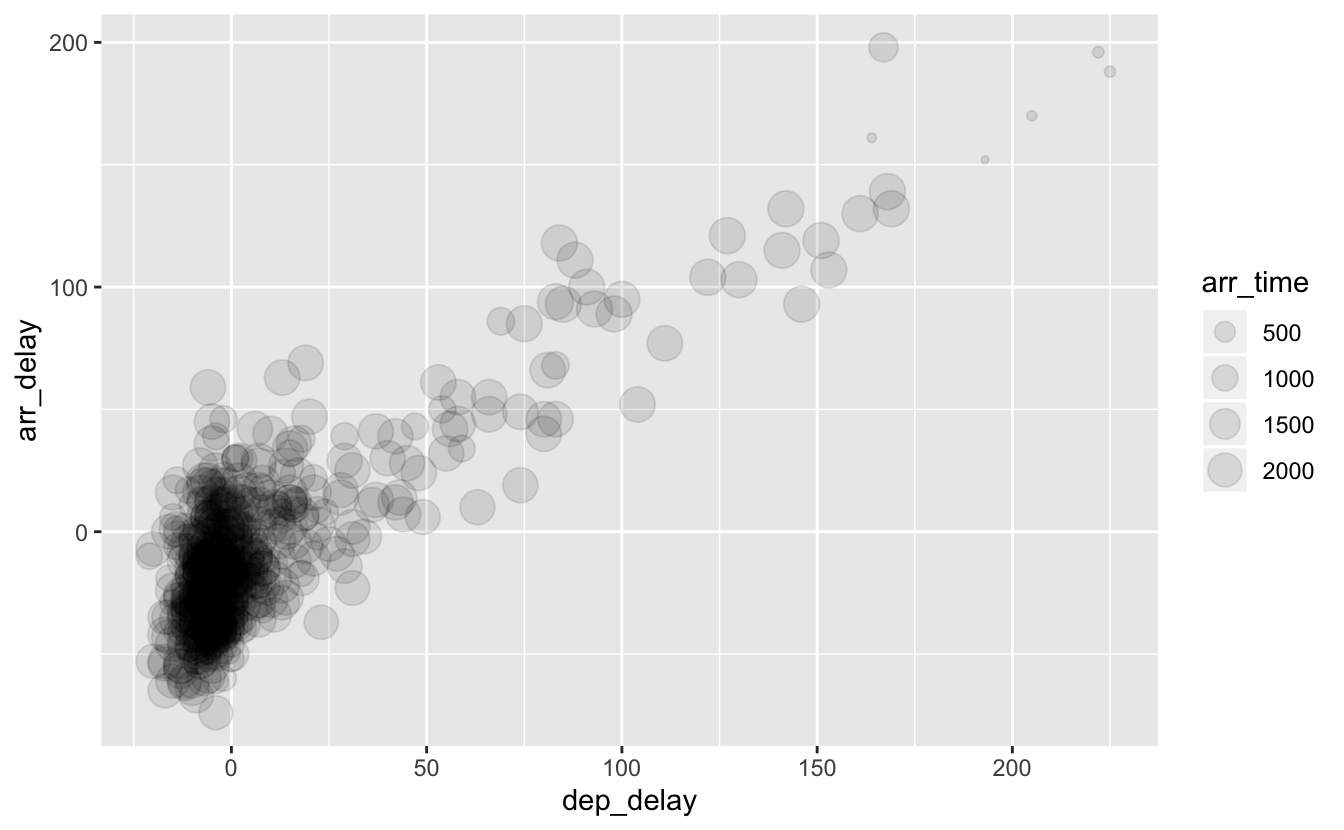
\includegraphics[width=0.9\linewidth]{figure/sizeplot-1} 

}

\caption{Association d'une variable continue à la taille des symboles avec l'argument `size`.}\label{fig:sizeplot}
\end{figure}

Si l'over-plotting est ici très important (c'est pourquoi j'ai utilisé \texttt{alpha}), on constate néanmoins que les vols avec les retards les plus importants sont presque tous arrivés très tôt dans la journée (``500'' signifie 5h00 du matin). Il s'agit probablement de vols qui devaient arriver dans la nuit, avant minuit, et qui sont finalement arrivés en tout début de journée, entre 00h01 et 5h00 du matin. Comme pour les autres arguments, il est possible d'utiliser \texttt{size} avec une valeur fixe, la même pour tous les symboles, lorsque cet argument n'est pas associé à une variable.

Enfin un conseil : évitez de trop surcharger vos graphiques. En combinant l'ensemble de ces arguments, il est malheureusement très facile d'obtenir des graphiques peu lisibles, ou contenant tellement d'informations qu'ils en deviennent difficiles à déchiffrer. Faites preuve de modération :

\begin{Shaded}
\begin{Highlighting}[]
\KeywordTok{ggplot}\NormalTok{(}\DataTypeTok{data =}\NormalTok{ alaska_flights, }
       \DataTypeTok{mapping =} \KeywordTok{aes}\NormalTok{(}\DataTypeTok{x =}\NormalTok{ dep_delay, }\DataTypeTok{y =}\NormalTok{ arr_delay, }\DataTypeTok{size =}\NormalTok{ arr_time)) }\OperatorTok{+}
\StringTok{  }\KeywordTok{geom_point}\NormalTok{(}\DataTypeTok{alpha =} \FloatTok{0.6}\NormalTok{, }
             \DataTypeTok{shape =} \DecValTok{22}\NormalTok{,}
             \DataTypeTok{color =} \StringTok{"orange"}\NormalTok{,}
             \DataTypeTok{fill =} \StringTok{"steelblue"}\NormalTok{,}
             \DataTypeTok{stroke =} \DecValTok{2}\NormalTok{)}
\end{Highlighting}
\end{Shaded}

\begin{figure}[htpb]

{\centering 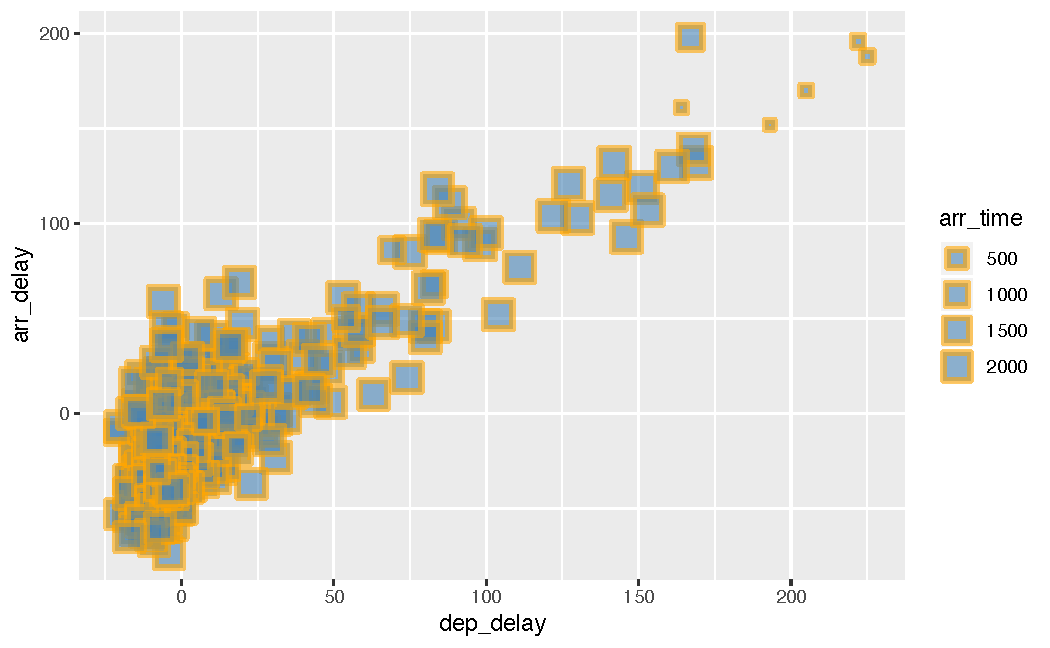
\includegraphics[width=0.9\linewidth]{figure/badplot-1} 

}

\caption{Sometimes, less is more!}\label{fig:badplot}
\end{figure}

\hypertarget{exercices-3}{%
\subsubsection{Exercices}\label{exercices-3}}

\begin{enumerate}
\def\labelenumi{\arabic{enumi}.}
\item
  À quoi sert l'argument \texttt{stroke} ?
\item
  Avec le jeu de données \texttt{diamonds}, tapez les commandes suivantes pour créer un nouveau tableau \texttt{diams} contenant moins de lignes (5000 au lieu de près de 54000) :
\end{enumerate}

\begin{Shaded}
\begin{Highlighting}[]
\KeywordTok{library}\NormalTok{(dplyr)}
\KeywordTok{set.seed}\NormalTok{(}\DecValTok{4532}\NormalTok{) }\CommentTok{# Afin que tout le monde récupère les mêmes lignes}
\NormalTok{diams <-}\StringTok{ }\NormalTok{diamonds }\OperatorTok\StringTok{ }
\StringTok{  }\KeywordTok{sample_n}\NormalTok{(}\DecValTok{5000}\NormalTok{)}
\end{Highlighting}
\end{Shaded}

\begin{enumerate}
\def\labelenumi{\arabic{enumi}.}
\setcounter{enumi}{2}
\tightlist
\item
  Avec ce nouveau tableau \texttt{diams}, tapez le code permettant de créer le graphique \ref{fig:exodiamonds} (Indice : affichez le tableau \texttt{diams} dans la console afin de voir quelles sont les variables disponibles).
\end{enumerate}

\begin{figure}[htpb]

{\centering 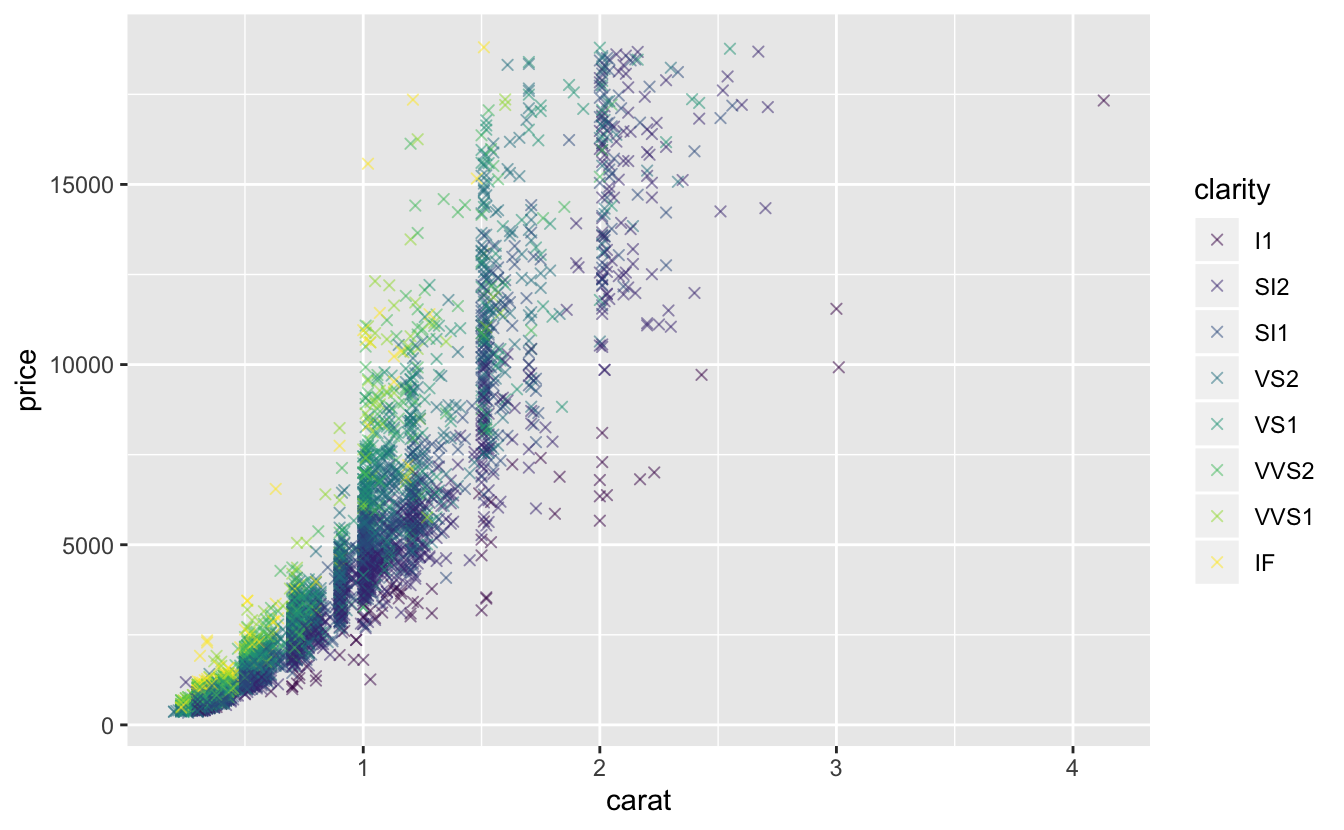
\includegraphics[width=0.9\linewidth]{figure/exodiamonds-1} 

}

\caption{Prix de 5000 diamants en fonction de leur taille en carats et de leur clarté.}\label{fig:exodiamonds}
\end{figure}

\begin{enumerate}
\def\labelenumi{\arabic{enumi}.}
\setcounter{enumi}{3}
\tightlist
\item
  Selon vous, à quoi sont dues les bandes verticales que l'on observe sur ce graphique ?
\end{enumerate}

\begin{center}\rule{0.5\linewidth}{0.5pt}\end{center}

\hypertarget{les-graphiques-en-lignes}{%
\subsection{Les graphiques en lignes}\label{les-graphiques-en-lignes}}

\hypertarget{un-nouveau-jeu-de-donnuxe9es}{%
\subsubsection{Un nouveau jeu de données}\label{un-nouveau-jeu-de-donnuxe9es}}

Les graphiques en ligne, ou ``linegraphs'' sont généralement utilisés lorsque l'axe des \texttt{x} porte une information \textbf{temporelle}, et l'axe des \texttt{y} une autre variable numérique. Le temps est une variable naturellement ordonnée : les jours, semaines, mois, années, se suivent naturellement. Les graphiques en lignes devraient être évités lorsqu'il n'y a pas une organisation séquentielle évidente de la variable portée par l'axe des \texttt{x}.

Concentrons nous maintenant sur le tableau \texttt{weather} du package \texttt{nycflights13}. Explorez ce tableau en appliquant les méthodes vues dans le chapitre \ref{dataset}. N'oubliez pas de consultez l'aide de ce jeu de données.

\begin{Shaded}
\begin{Highlighting}[]
\NormalTok{weather}
\end{Highlighting}
\end{Shaded}

\begin{verbatim}
# A tibble: 26,115 x 15
   origin  year month   day  hour  temp  dewp humid wind_dir
   <chr>  <int> <int> <int> <int> <dbl> <dbl> <dbl>    <dbl>
 1 EWR     2013     1     1     1  39.0  26.1  59.4      270
 2 EWR     2013     1     1     2  39.0  27.0  61.6      250
 3 EWR     2013     1     1     3  39.0  28.0  64.4      240
 4 EWR     2013     1     1     4  39.9  28.0  62.2      250
 5 EWR     2013     1     1     5  39.0  28.0  64.4      260
 6 EWR     2013     1     1     6  37.9  28.0  67.2      240
 7 EWR     2013     1     1     7  39.0  28.0  64.4      240
 8 EWR     2013     1     1     8  39.9  28.0  62.2      250
 9 EWR     2013     1     1     9  39.9  28.0  62.2      260
10 EWR     2013     1     1    10  41    28.0  59.6      260
# ... with 26,105 more rows, and 6 more variables: wind_speed <dbl>,
#   wind_gust <dbl>, precip <dbl>, pressure <dbl>, visib <dbl>,
#   time_hour <dttm>
\end{verbatim}

Nous allons nous intéresser à la variable \texttt{temp}, qui contient un enregistrement de température pour chaque heure de chaque jour de 2013 pour les 3 aéroports de New York. Cela représente une grande quantité de données, aussi, nous nous limiterons aux températures observées entre le premier et le 15 janvier, pour l'aéroport Newark uniquement.

\begin{Shaded}
\begin{Highlighting}[]
\NormalTok{small_weather <-}\StringTok{ }\NormalTok{weather }\OperatorTok\StringTok{ }
\StringTok{  }\KeywordTok{filter}\NormalTok{(origin }\OperatorTok{==}\StringTok{ "EWR"}\NormalTok{,}
\NormalTok{         month }\OperatorTok{==}\StringTok{ }\DecValTok{1}\NormalTok{,}
\NormalTok{         day }\OperatorTok{<=}\StringTok{ }\DecValTok{15}\NormalTok{)}
\end{Highlighting}
\end{Shaded}

La fonction \texttt{filter()} fonctionne sur le même principe que la fonction \texttt{subset()} découverte dans les tutoriels de DataCamp. Ici, nous demandons à R de créer un nouveau tableau de données, nommé \texttt{small\_weather}, qui ne contiendra que les lignes correspondant à \texttt{origin\ ==\ "EWR"}, \texttt{month\ ==\ 1} et \texttt{day\ \textless{}=\ 15}, c'est à dire les données météorologiques de l'aéroport de Newark pour les 15 premiers jours de janvier 2013.

\hypertarget{exercice}{%
\subsubsection{Exercice}\label{exercice}}

Avec \texttt{View()}, consultez le tableau nouvellement créé. Expliquez pourquoi la variable \texttt{time\_hour} identifie de manière unique le moment ou chaque mesure a été réalisée alors que ce n'est pas le cas de la variable \texttt{hour}.

\hypertarget{la-fonction-geom_line}{%
\subsubsection{\texorpdfstring{La fonction \texttt{geom\_line()}}{La fonction geom\_line()}}\label{la-fonction-geom_line}}

Les line graphs sont produits de la même façon que les nuages de points. Seul l'objet géométrique permettant de visualiser les données change. Au lieu d'utiliser \texttt{geom\_point()}, on utilisera \texttt{geom\_line()} :

\begin{Shaded}
\begin{Highlighting}[]
\KeywordTok{ggplot}\NormalTok{(}\DataTypeTok{data =}\NormalTok{ small_weather, }\DataTypeTok{mapping =} \KeywordTok{aes}\NormalTok{(}\DataTypeTok{x =}\NormalTok{ time_hour, }\DataTypeTok{y =}\NormalTok{ temp)) }\OperatorTok{+}
\StringTok{  }\KeywordTok{geom_line}\NormalTok{()}
\end{Highlighting}
\end{Shaded}

\begin{figure}[htpb]

{\centering 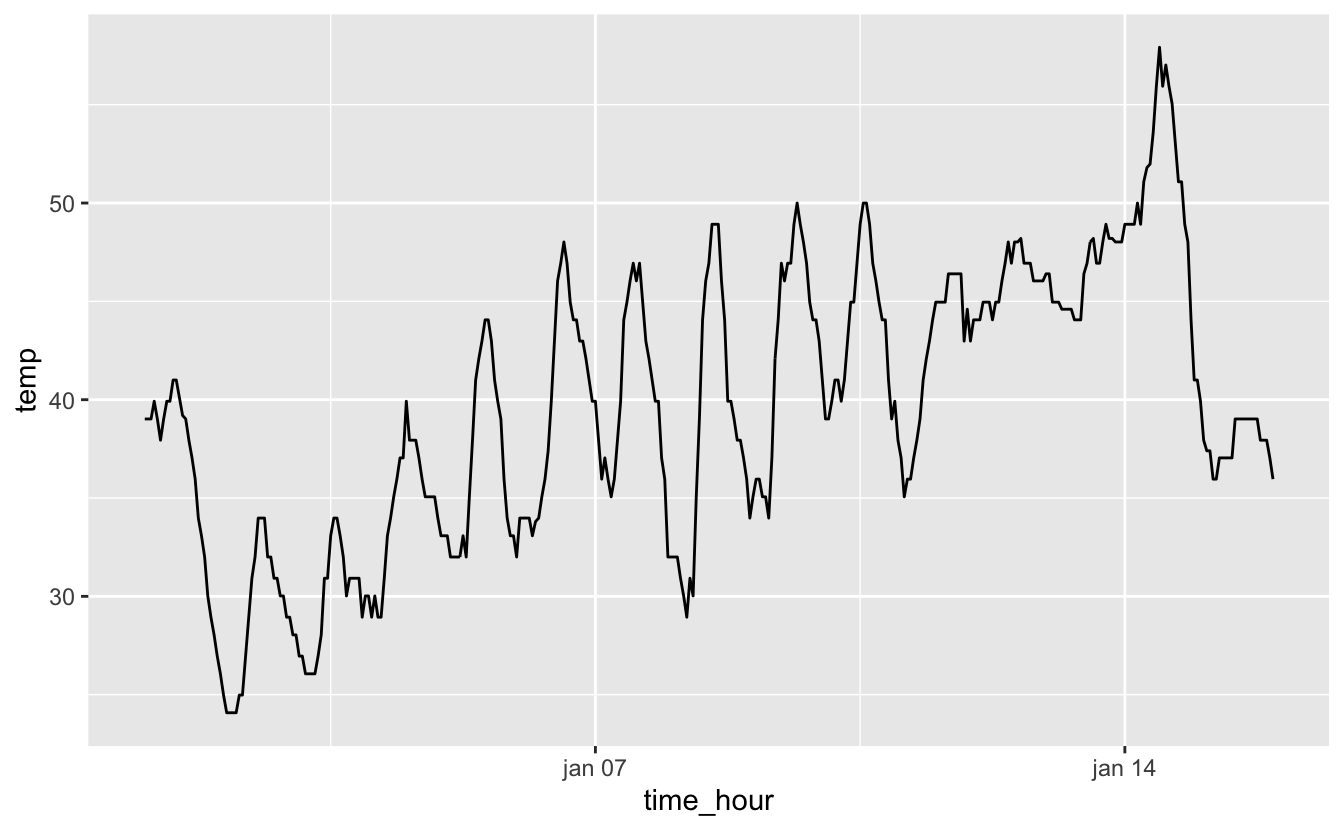
\includegraphics[width=0.9\linewidth]{figure/linegraph-1} 

}

\caption{Températures horaires à l'aéroport de Newark entre le 1er et le 15 janvier 2013.}\label{fig:linegraph}
\end{figure}

Très logiquement, on observe des oscillations plus ou moins régulières qui correspondent à l'alternance jour/nuit. Notez l'échelle de l'axe des ordonnées : les températures sont enregistrées en degrés Farenheit.

Nous connaissons maintenant 2 types d'objets \texttt{geom}étriques : les points et les lignes. Il est tout à fait possible d'ajouter plusieurs couches à un graphique, chacune d'elle correspondant à un objet \texttt{geom}étrique différent (voir figure \ref{fig:lineplotgraph}) :

\begin{Shaded}
\begin{Highlighting}[]
\KeywordTok{ggplot}\NormalTok{(}\DataTypeTok{data =}\NormalTok{ small_weather, }\DataTypeTok{mapping =} \KeywordTok{aes}\NormalTok{(}\DataTypeTok{x =}\NormalTok{ time_hour, }\DataTypeTok{y =}\NormalTok{ temp)) }\OperatorTok{+}
\StringTok{  }\KeywordTok{geom_line}\NormalTok{() }\OperatorTok{+}
\StringTok{  }\KeywordTok{geom_point}\NormalTok{()}
\end{Highlighting}
\end{Shaded}

\begin{figure}[htpb]

{\centering 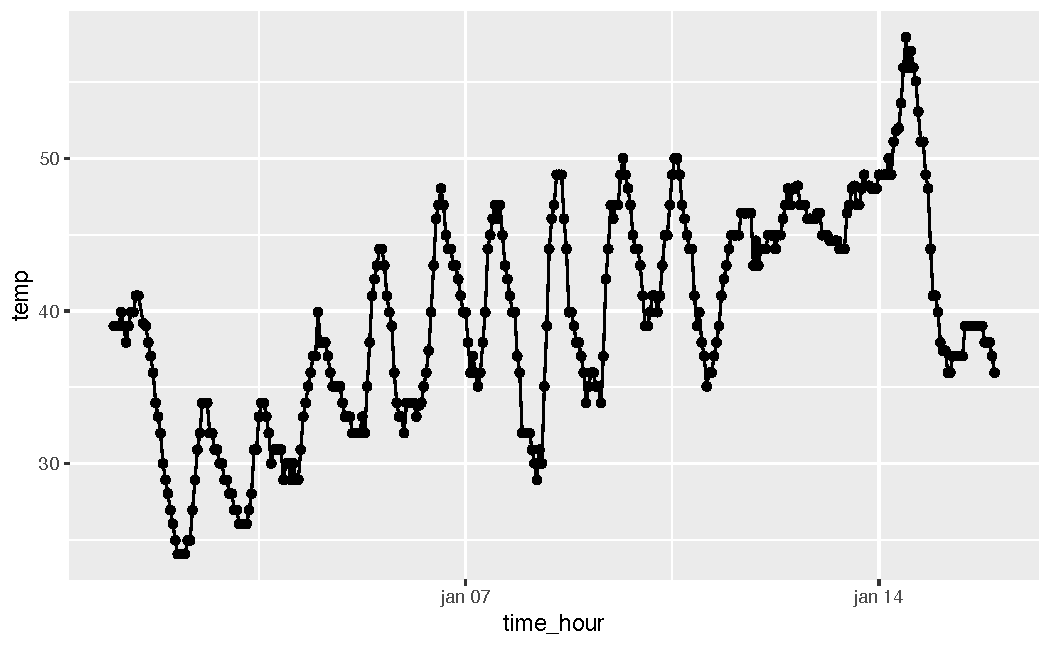
\includegraphics[width=0.9\linewidth]{figure/lineplotgraph-1} 

}

\caption{Températures horaires à l'aéroport de Newark entre le 1er et le 15 janvier 2013.}\label{fig:lineplotgraph}
\end{figure}

Enfin, comme pour les points, il est possible de spécifier plusieurs caractéristiques esthétiques des lignes, soit en les associant à des variables, au sein de la fonction \texttt{aes()}, soit en les utilisant en guise de paramètres pour modifier l'aspect général. Les arguments les plus classiques sont une fois de plus \texttt{color} (ou \texttt{colour}) pour modifier la couleur des lignes, \texttt{linetype} pour modifier le type de lignes (continues, pointillées, tirets, etc), et \texttt{size} pour modifier l'épaisseur des lignes.

Reprenons le jeu de données complet \texttt{weather}, et filtrons uniquement les dates comprises entre le premier et le 15 janvier, mais cette fois pour les 3 aéroports de New York :

\begin{Shaded}
\begin{Highlighting}[]
\NormalTok{small_weather_airports <-}\StringTok{ }\NormalTok{weather }\OperatorTok\StringTok{ }
\StringTok{  }\KeywordTok{filter}\NormalTok{(month }\OperatorTok{==}\StringTok{ }\DecValTok{1}\NormalTok{,}
\NormalTok{         day }\OperatorTok{<=}\StringTok{ }\DecValTok{15}\NormalTok{)}
\end{Highlighting}
\end{Shaded}

Nous pouvons maintenant réaliser un ``linegraph'' sur lequel une courbe apparaîtra pour chaque aéroport. Pour cela, nous devons associer la variable \texttt{origin} à un attribut esthétique des lignes. Par exemple (figure \ref{fig:linecolor}) :

\begin{Shaded}
\begin{Highlighting}[]
\KeywordTok{ggplot}\NormalTok{(}\DataTypeTok{data =}\NormalTok{ small_weather_airports, }
       \DataTypeTok{mapping =} \KeywordTok{aes}\NormalTok{(}\DataTypeTok{x =}\NormalTok{ time_hour, }\DataTypeTok{y =}\NormalTok{ temp)) }\OperatorTok{+}
\StringTok{  }\KeywordTok{geom_line}\NormalTok{(}\KeywordTok{aes}\NormalTok{(}\DataTypeTok{color =}\NormalTok{ origin))}
\end{Highlighting}
\end{Shaded}

\begin{figure}[htpb]

{\centering 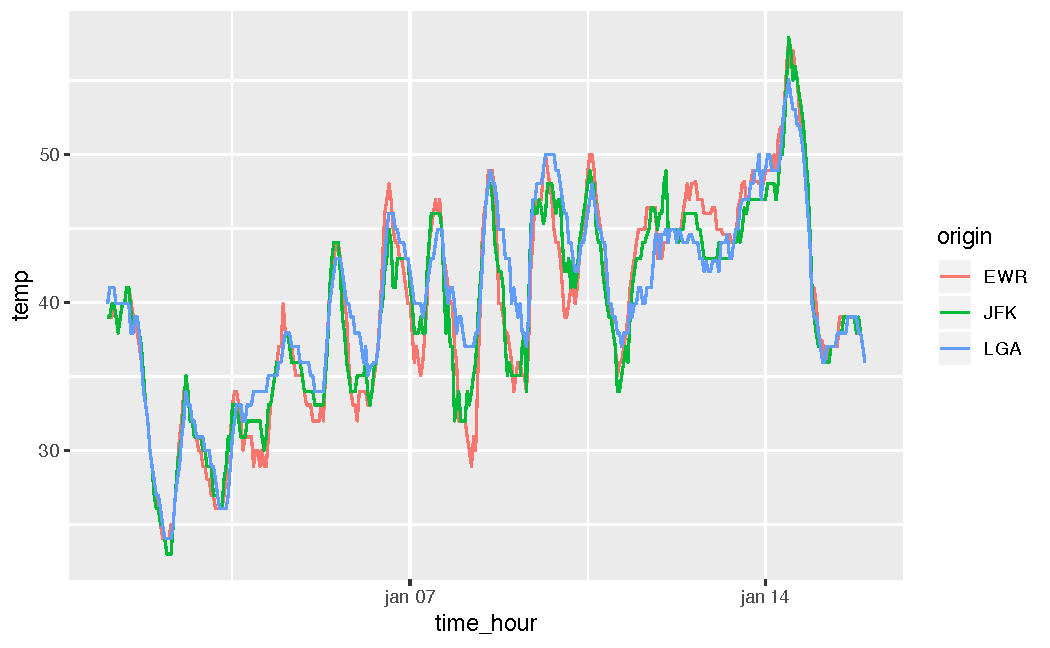
\includegraphics[width=0.9\linewidth]{figure/linecolor-1} 

}

\caption{Températures horaires des 3 aéroports de New York entre le 1er et le 15 janvier 2013.}\label{fig:linecolor}
\end{figure}

Ou bien (figure \ref{fig:linetype}) :

\begin{Shaded}
\begin{Highlighting}[]
\KeywordTok{ggplot}\NormalTok{(}\DataTypeTok{data =}\NormalTok{ small_weather_airports, }
       \DataTypeTok{mapping =} \KeywordTok{aes}\NormalTok{(}\DataTypeTok{x =}\NormalTok{ time_hour, }\DataTypeTok{y =}\NormalTok{ temp)) }\OperatorTok{+}
\StringTok{  }\KeywordTok{geom_line}\NormalTok{(}\KeywordTok{aes}\NormalTok{(}\DataTypeTok{linetype =}\NormalTok{ origin))}
\end{Highlighting}
\end{Shaded}

\begin{figure}[htpb]

{\centering 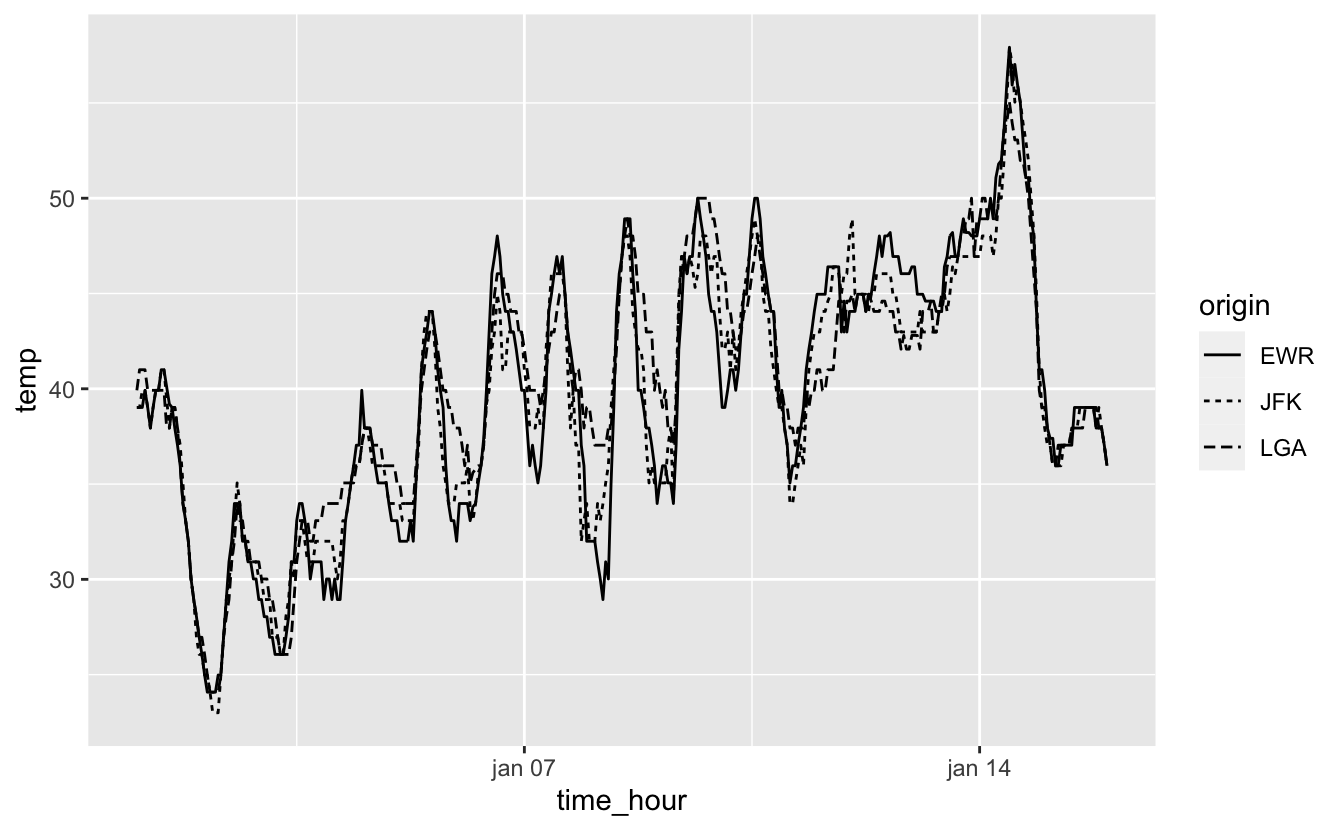
\includegraphics[width=0.9\linewidth]{figure/linetype-1} 

}

\caption{Températures horaires des 3 aéroports de New York entre le 1er et le 15 janvier 2013.}\label{fig:linetype}
\end{figure}

Ou encore (figure \ref{fig:linetypecolor}) :

\begin{Shaded}
\begin{Highlighting}[]
\KeywordTok{ggplot}\NormalTok{(}\DataTypeTok{data =}\NormalTok{ small_weather_airports, }
       \DataTypeTok{mapping =} \KeywordTok{aes}\NormalTok{(}\DataTypeTok{x =}\NormalTok{ time_hour, }\DataTypeTok{y =}\NormalTok{ temp)) }\OperatorTok{+}
\StringTok{  }\KeywordTok{geom_line}\NormalTok{(}\KeywordTok{aes}\NormalTok{(}\DataTypeTok{color =}\NormalTok{ origin, }\DataTypeTok{linetype =}\NormalTok{ origin))}
\end{Highlighting}
\end{Shaded}

\begin{figure}[htpb]

{\centering 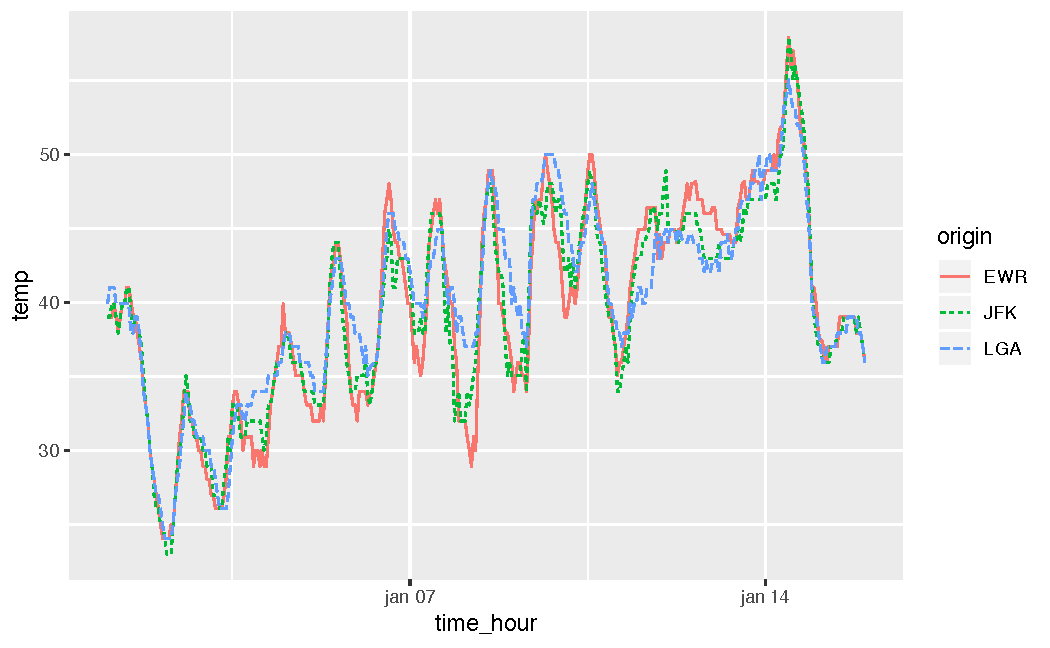
\includegraphics[width=0.9\linewidth]{figure/linetypecolor-1} 

}

\caption{Températures horaires des 3 aéroports de New York entre le 1er et le 15 janvier 2013.}\label{fig:linetypecolor}
\end{figure}

\hypertarget{uxe0-quel-endroit-placer-aes-et-les-arguments-color-size-etc.}{%
\subsubsection{\texorpdfstring{À quel endroit placer \texttt{aes()} et les arguments \texttt{color}, \texttt{size}, etc. ?}{À quel endroit placer aes() et les arguments color, size, etc. ?}}\label{uxe0-quel-endroit-placer-aes-et-les-arguments-color-size-etc.}}

Jusqu'à maintenant, pour spécifier les associations entre certaines variables et les caractéristiques esthétiques d'un graphique, nous avons été amenés à utiliser la fonction \texttt{aes()} à 2 endroits distincts :

\begin{enumerate}
\def\labelenumi{\arabic{enumi}.}
\tightlist
\item
  au sein de la fonction \texttt{ggplot()}
\item
  au sein des fonctions \texttt{geom\_XXX()}
\end{enumerate}

Comment choisir l'endroit où renseigner \texttt{aes()} ? Pour bien comprendre, reprenons l'exemple du graphique \ref{fig:lineplotgraph} sur lequel nous avions ajouté 2 couches contenant chacune un objet géométrique différent (afin de gagner de la place, j'omets volontairement le nom des arguments \texttt{data} et \texttt{mapping} dans la fonction \texttt{ggplot()}) :

\begin{Shaded}
\begin{Highlighting}[]
\KeywordTok{ggplot}\NormalTok{(small_weather, }\KeywordTok{aes}\NormalTok{(}\DataTypeTok{x =}\NormalTok{ time_hour, }\DataTypeTok{y =}\NormalTok{ temp)) }\OperatorTok{+}
\StringTok{  }\KeywordTok{geom_line}\NormalTok{() }\OperatorTok{+}
\StringTok{  }\KeywordTok{geom_point}\NormalTok{()}
\end{Highlighting}
\end{Shaded}

\begin{figure}[htpb]

{\centering 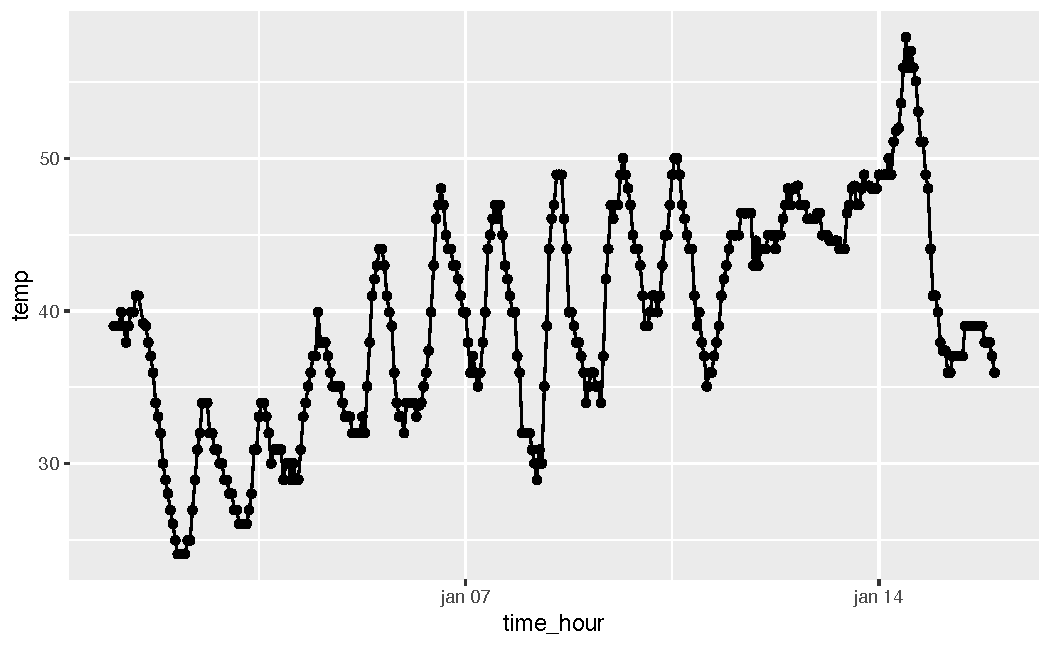
\includegraphics[width=0.9\linewidth]{figure/lineplotgraph2-1} 

}

\caption{Températures horaires à l'aéroport de Newark entre le 1er et le 15 janvier 2013.}\label{fig:lineplotgraph2}
\end{figure}

Voyons ce qui se passe si on associe la variable \texttt{wind\_speed} à l'esthétique \texttt{color}, à plusieurs endroits du code ci-dessus. Comparez les trois syntaxes et observez les différences entre les 3 graphiques obtenus :

\begin{Shaded}
\begin{Highlighting}[]
\KeywordTok{ggplot}\NormalTok{(small_weather, }\KeywordTok{aes}\NormalTok{(}\DataTypeTok{x =}\NormalTok{ time_hour, }\DataTypeTok{y =}\NormalTok{ temp, }\DataTypeTok{color =}\NormalTok{ wind_speed)) }\OperatorTok{+}
\StringTok{  }\KeywordTok{geom_line}\NormalTok{() }\OperatorTok{+}
\StringTok{  }\KeywordTok{geom_point}\NormalTok{()}
\end{Highlighting}
\end{Shaded}

\begin{figure}[htpb]

{\centering 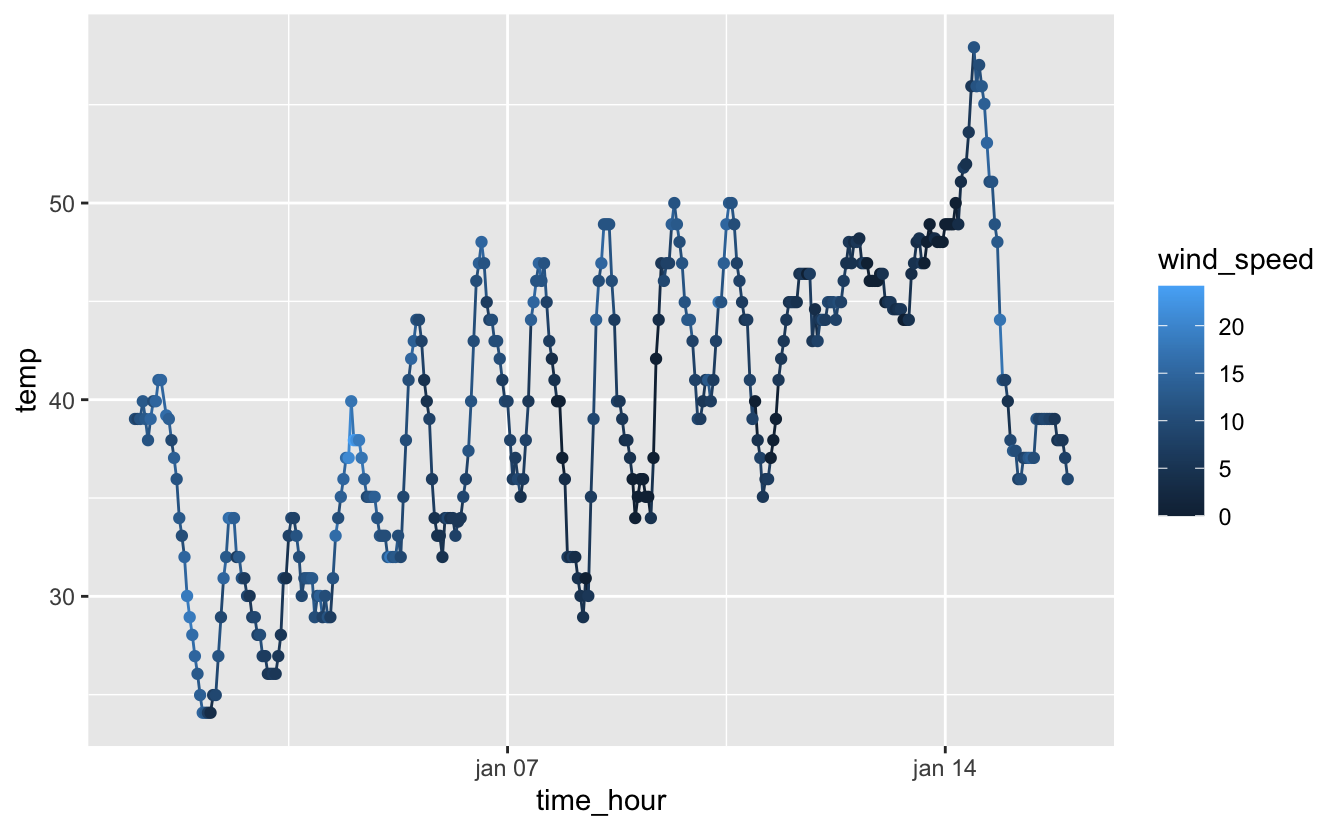
\includegraphics[width=0.9\linewidth]{figure/wind-1} 

}

\caption{Températures horaires et vitesse du vent à l'aéroport de Newark entre le 1er et le 15 janvier 2013. La couleur de la ligne et des points renseigne sur la vitesse du vent.}\label{fig:wind}
\end{figure}

\begin{Shaded}
\begin{Highlighting}[]
\KeywordTok{ggplot}\NormalTok{(small_weather, }\KeywordTok{aes}\NormalTok{(}\DataTypeTok{x =}\NormalTok{ time_hour, }\DataTypeTok{y =}\NormalTok{ temp)) }\OperatorTok{+}
\StringTok{  }\KeywordTok{geom_line}\NormalTok{(}\KeywordTok{aes}\NormalTok{(}\DataTypeTok{color =}\NormalTok{ wind_speed)) }\OperatorTok{+}
\StringTok{  }\KeywordTok{geom_point}\NormalTok{()}
\end{Highlighting}
\end{Shaded}

\begin{figure}[htpb]

{\centering 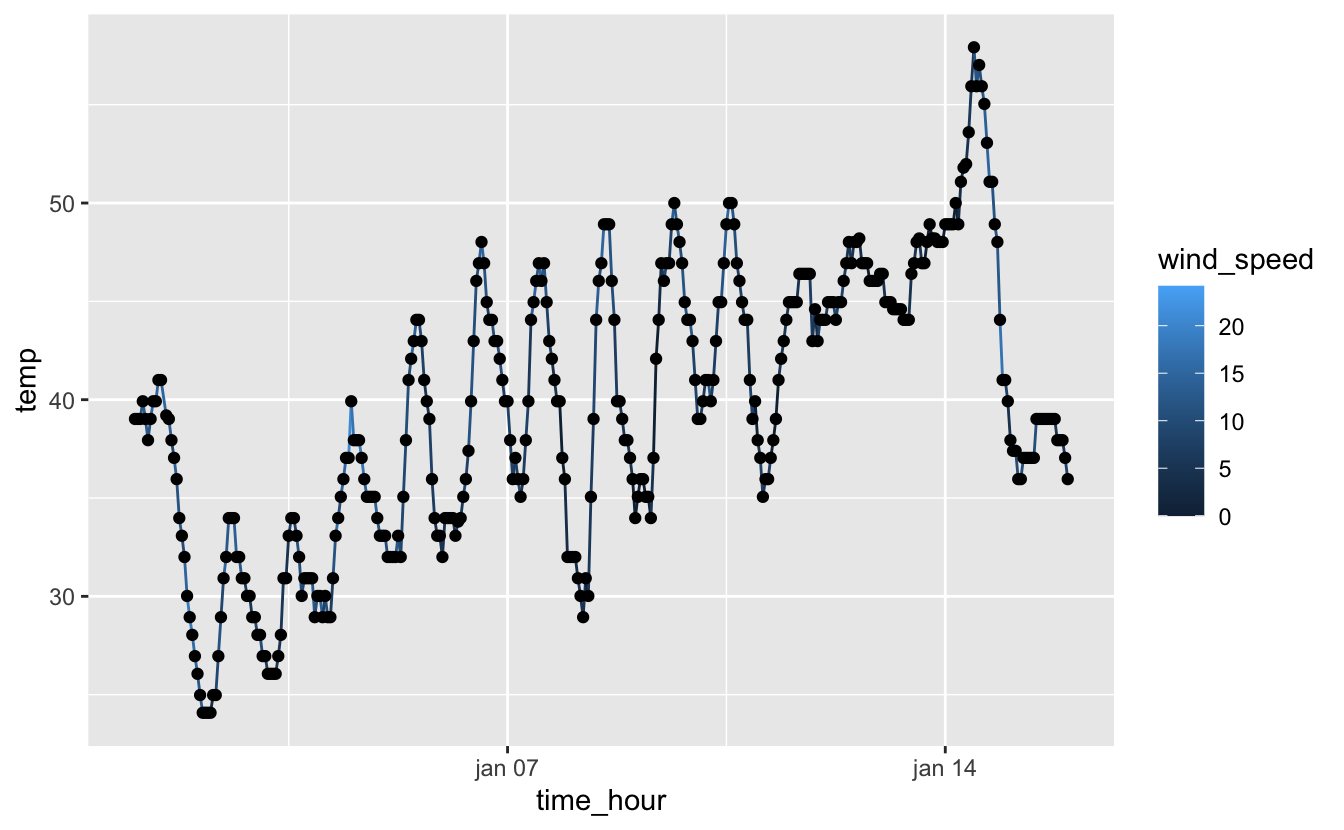
\includegraphics[width=0.9\linewidth]{figure/wind2-1} 

}

\caption{Températures horaires et vitesse du vent à l'aéroport de Newark entre le 1er et le 15 janvier 2013. La couleur de la ligne renseigne sur la vitesse du vent.}\label{fig:wind2}
\end{figure}

\begin{Shaded}
\begin{Highlighting}[]
\KeywordTok{ggplot}\NormalTok{(small_weather, }\KeywordTok{aes}\NormalTok{(}\DataTypeTok{x =}\NormalTok{ time_hour, }\DataTypeTok{y =}\NormalTok{ temp)) }\OperatorTok{+}
\StringTok{  }\KeywordTok{geom_line}\NormalTok{() }\OperatorTok{+}
\StringTok{  }\KeywordTok{geom_point}\NormalTok{(}\KeywordTok{aes}\NormalTok{(}\DataTypeTok{color =}\NormalTok{ wind_speed))}
\end{Highlighting}
\end{Shaded}

\begin{figure}[htpb]

{\centering 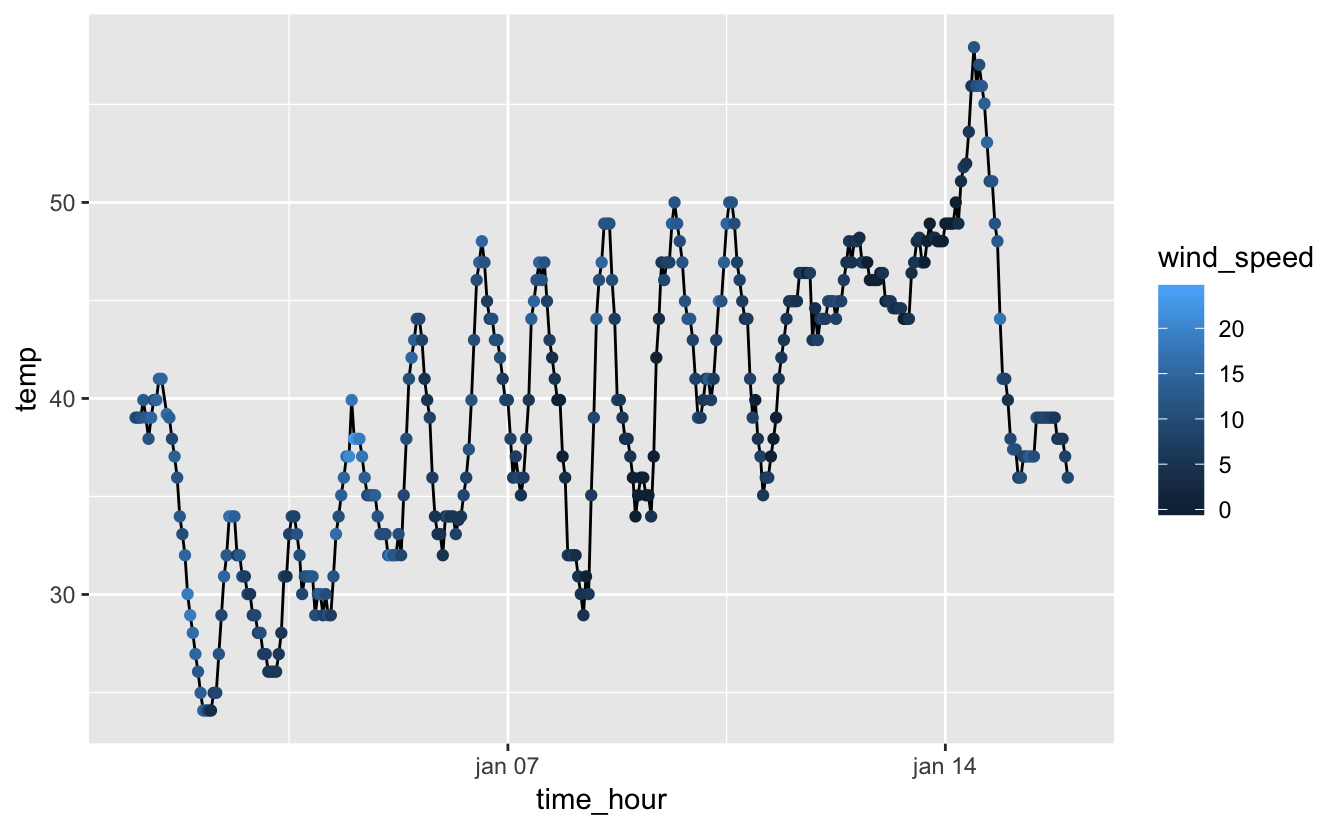
\includegraphics[width=0.9\linewidth]{figure/wind3-1} 

}

\caption{Températures horaires et vitesse du vent à l'aéroport de Newark entre le 1er et le 15 janvier 2013. La couleur des points renseigne sur la vitesse du vent.}\label{fig:wind3}
\end{figure}

Vous l'aurez compris, lorsque l'on spécifie \texttt{aes()} à l'intérieur de la fonction \texttt{ggplot()}, les associations de variables et d'esthétiques sont appliquées à tous les objets géométriques, donc à toutes les autres couches. En revanche, quand \texttt{aes()} est spécifié dans une couche donnée, les réglages ne s'appliquent qu'à cette couche spécifique.

En l'occurence, si le même réglage est spécifié dans la fonction \texttt{ggplot()} et dans une fonction \texttt{geom\_XXX()}, c'est le réglage spécifié dans l'objet géométrique qui l'emporte :

\begin{Shaded}
\begin{Highlighting}[]
\KeywordTok{ggplot}\NormalTok{(small_weather, }\KeywordTok{aes}\NormalTok{(}\DataTypeTok{x =}\NormalTok{ time_hour, }\DataTypeTok{y =}\NormalTok{ temp, }\DataTypeTok{color =}\NormalTok{ wind_speed)) }\OperatorTok{+}
\StringTok{  }\KeywordTok{geom_line}\NormalTok{(}\DataTypeTok{color =} \StringTok{"orange"}\NormalTok{) }\OperatorTok{+}
\StringTok{  }\KeywordTok{geom_point}\NormalTok{()}
\end{Highlighting}
\end{Shaded}

\begin{figure}[htpb]

{\centering 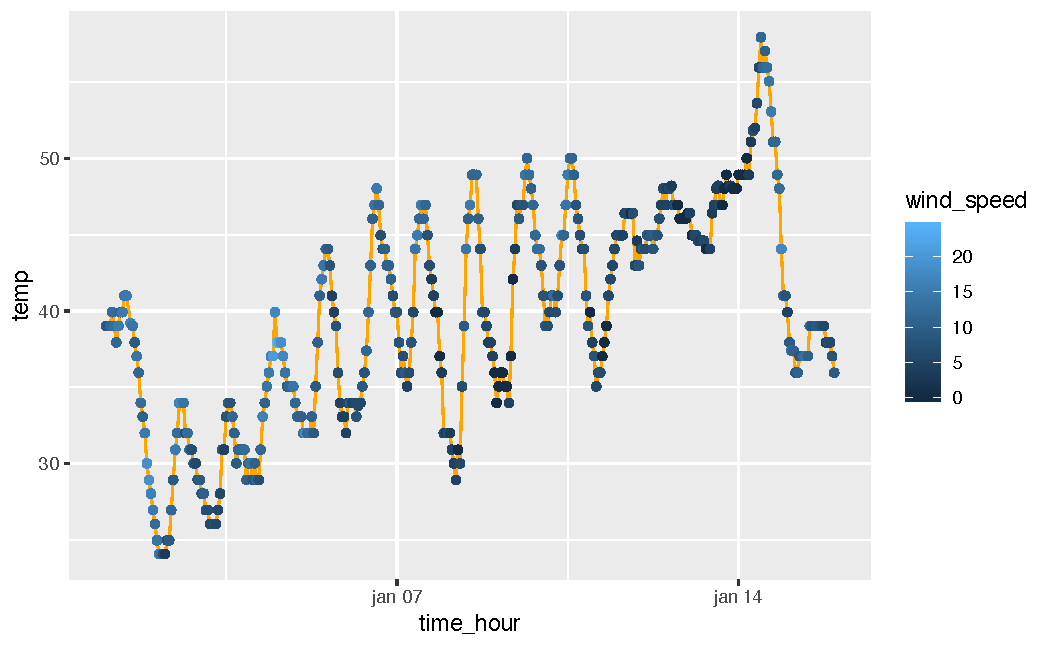
\includegraphics[width=0.9\linewidth]{figure/wind4-1} 

}

\caption{Températures horaires et vitesse du vent à l'aéroport de Newark entre le 1er et le 15 janvier 2013.}\label{fig:wind4}
\end{figure}

Il est ainsi possible de spécifier des éléments esthétiques qui s'appliqueront à toutes les couches d'un graphique, et d'autres qui ne s'appliqueront qu'à une couche spécifique, qu'à un objet géométrique particulier.

\begin{center}\rule{0.5\linewidth}{0.5pt}\end{center}

\hypertarget{histogram}{%
\subsection{Les histogrammes}\label{histogram}}

Un histogramme permet de visualiser la distribution \textbf{d'une variable} numérique continue. Contrairement aux deux types de graphiques vus précédemment, il sera donc inutile de préciser la variable à associer à l'axe des ordonnées : R la calcule automatiquement pour nous lorsque nous faisons appel à la fonction \texttt{geom\_histogram()} pour créer un objet géométrique ``histogramme''.

\hypertarget{lobjet-geom_histogram}{%
\subsubsection{\texorpdfstring{L'objet \texttt{geom\_histogram()}}{L'objet geom\_histogram()}}\label{lobjet-geom_histogram}}

Si on reprend le jeu de données \texttt{weather}, on peut par exemple s'intéresser à la distribution des températures tout au long de l'année :

\begin{Shaded}
\begin{Highlighting}[]
\KeywordTok{ggplot}\NormalTok{(weather, }\KeywordTok{aes}\NormalTok{(}\DataTypeTok{x =}\NormalTok{ temp)) }\OperatorTok{+}
\StringTok{  }\KeywordTok{geom_histogram}\NormalTok{()}
\end{Highlighting}
\end{Shaded}

\begin{verbatim}
`stat_bin()` using `bins = 30`. Pick better value with `binwidth`.
\end{verbatim}

\begin{figure}[htpb]

{\centering 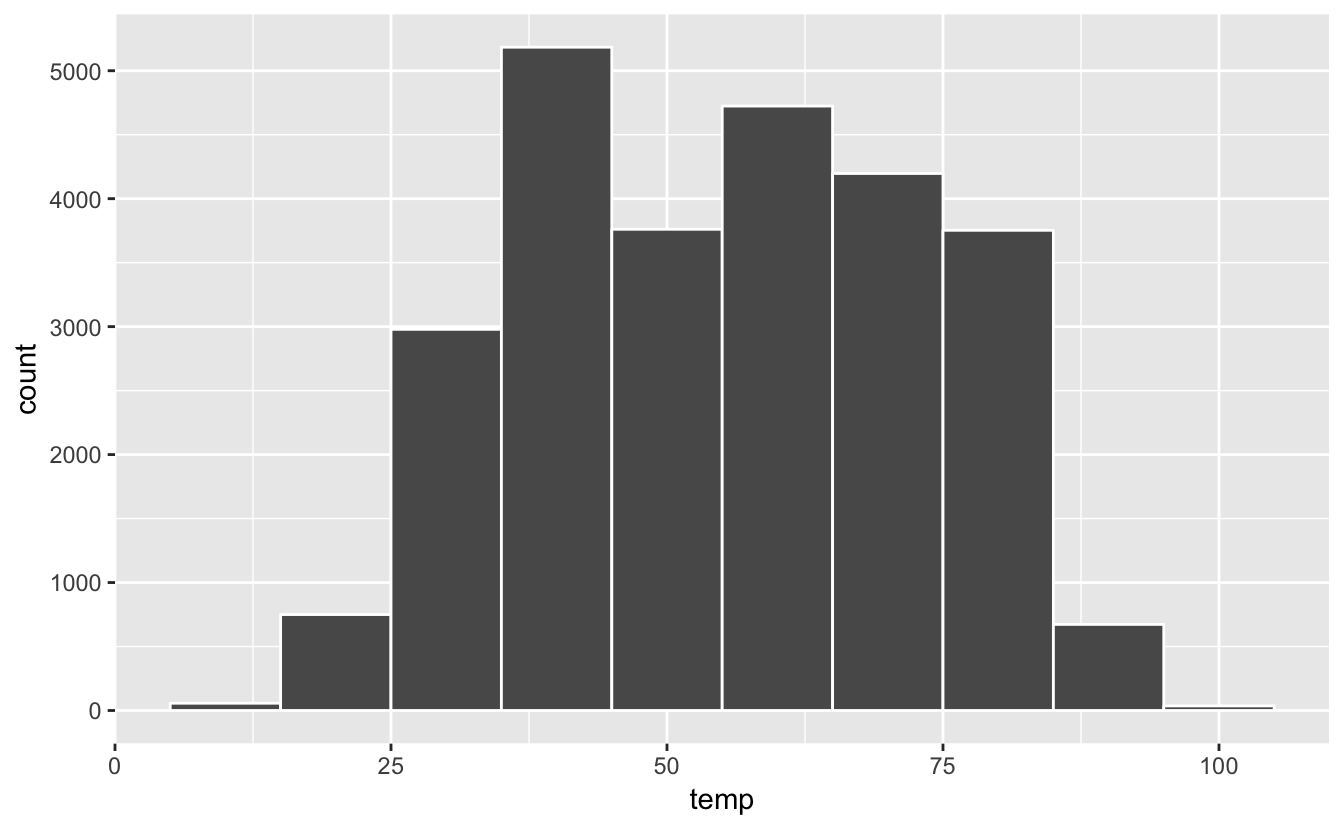
\includegraphics[width=0.9\linewidth]{figure/unnamed-chunk-47-1} 

}

\caption{Histogramme des températures enregistrées en 2013 dans les 3 aéroports de New York.}\label{fig:unnamed-chunk-47}
\end{figure}

On observe plusieurs choses :

\begin{enumerate}
\def\labelenumi{\arabic{enumi}.}
\tightlist
\item
  La distribution semble globalement bimodale avec un pic autour de 36-37 degrés Farenheit (2 à 3 ºC) et un autre autour de 65-70 degrés Farenheit (18-21 ºC).
\item
  Les températures ont varié entre 12 degrés Farenheit (-11ºC) et 100 degrés Farenheit (près de 38ºC).
\item
  R nous avertit qu'une valeur non finie n'a pas pu être intégrée.
\item
  R nous indique qu'il a choisi de représenter 30 classes de températures (\texttt{bins\ =\ 30}). C'est la valeur par défaut. R nous conseille de choisir une valeur plus appropriée.
\end{enumerate}

Comme pour les nuages de points utilisant les symboles 21 à 24, il est possible de spécifier la couleur de remplissage des barres avec l'argument \texttt{fill} et la couleur du contour des barres avec l'argument \texttt{color} :

\begin{Shaded}
\begin{Highlighting}[]
\KeywordTok{ggplot}\NormalTok{(weather, }\KeywordTok{aes}\NormalTok{(}\DataTypeTok{x =}\NormalTok{ temp)) }\OperatorTok{+}
\StringTok{  }\KeywordTok{geom_histogram}\NormalTok{(}\DataTypeTok{fill =} \StringTok{"steelblue"}\NormalTok{, }\DataTypeTok{color =} \StringTok{"grey80"}\NormalTok{)}
\end{Highlighting}
\end{Shaded}

\begin{figure}[htpb]

{\centering 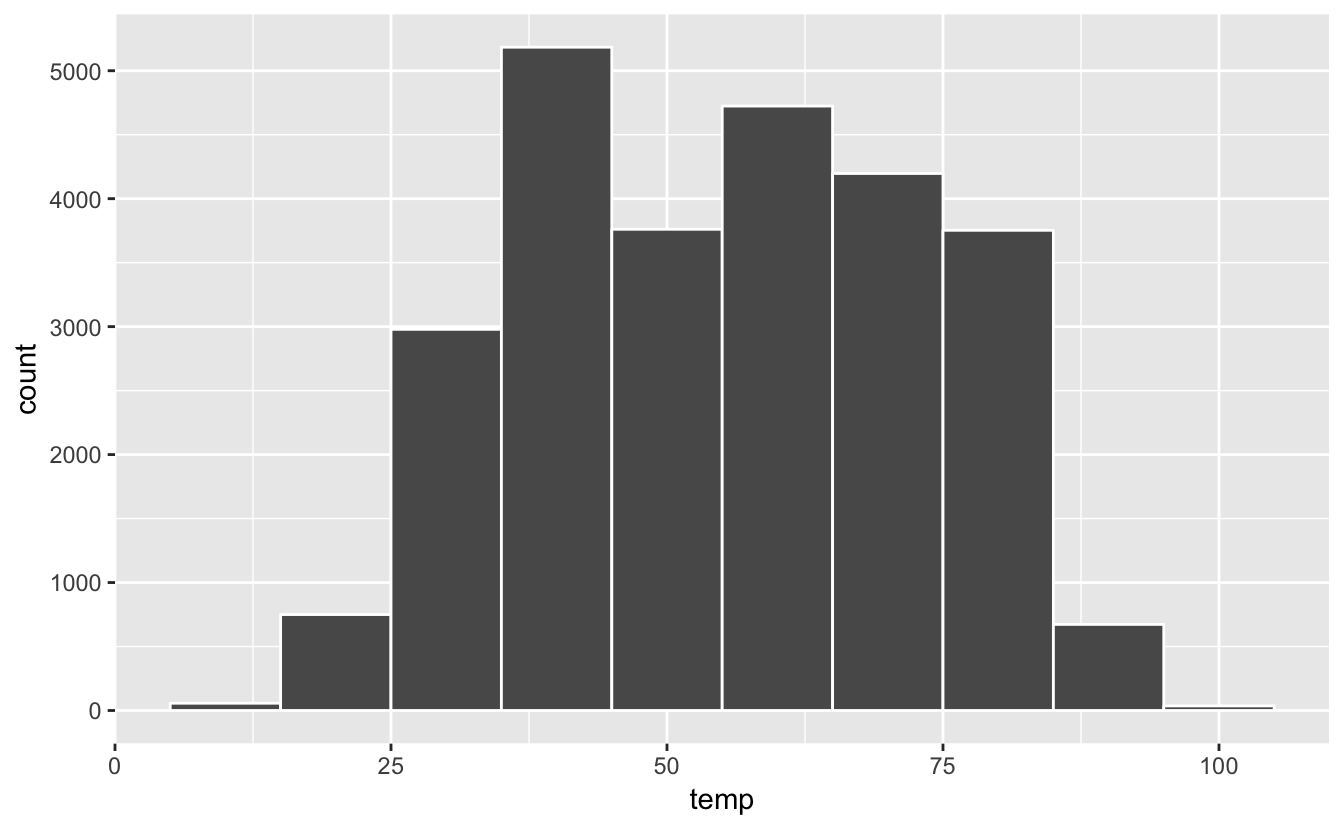
\includegraphics[width=0.9\linewidth]{figure/unnamed-chunk-48-1} 

}

\caption{Utilisation des arguments `fill` et `color` pour modifier l'aspect de l'histogramme.}\label{fig:unnamed-chunk-48}
\end{figure}

\hypertarget{la-taille-des-classes}{%
\subsubsection{La taille des classes}\label{la-taille-des-classes}}

Par défaut, R choisit arbitrairement de représenter 30 classes. Ce n'est que rarement le bon choix, et il est souvent nécessaire de tâtonner pour trouver le nombre de classes approprié : celui qui permet d'avoir une idée correcte de la distribution des données.

Il est possible d'ajuster les caractéristiques des classes de l'histogramme de l'une des 3 façons suivantes :

\begin{enumerate}
\def\labelenumi{\arabic{enumi}.}
\tightlist
\item
  En ajustant le nombre de classes avec \texttt{bins}.
\item
  En précisant la largeur des classes avec \texttt{binwidth}.
\item
  En fournissant manuellement les limites des classes avec \texttt{breaks}.
\end{enumerate}

\begin{Shaded}
\begin{Highlighting}[]
\KeywordTok{ggplot}\NormalTok{(weather, }\KeywordTok{aes}\NormalTok{(}\DataTypeTok{x =}\NormalTok{ temp)) }\OperatorTok{+}
\StringTok{  }\KeywordTok{geom_histogram}\NormalTok{(}\DataTypeTok{bins =} \DecValTok{60}\NormalTok{, }\DataTypeTok{color =} \StringTok{"white"}\NormalTok{)}
\end{Highlighting}
\end{Shaded}

\begin{figure}[htpb]

{\centering 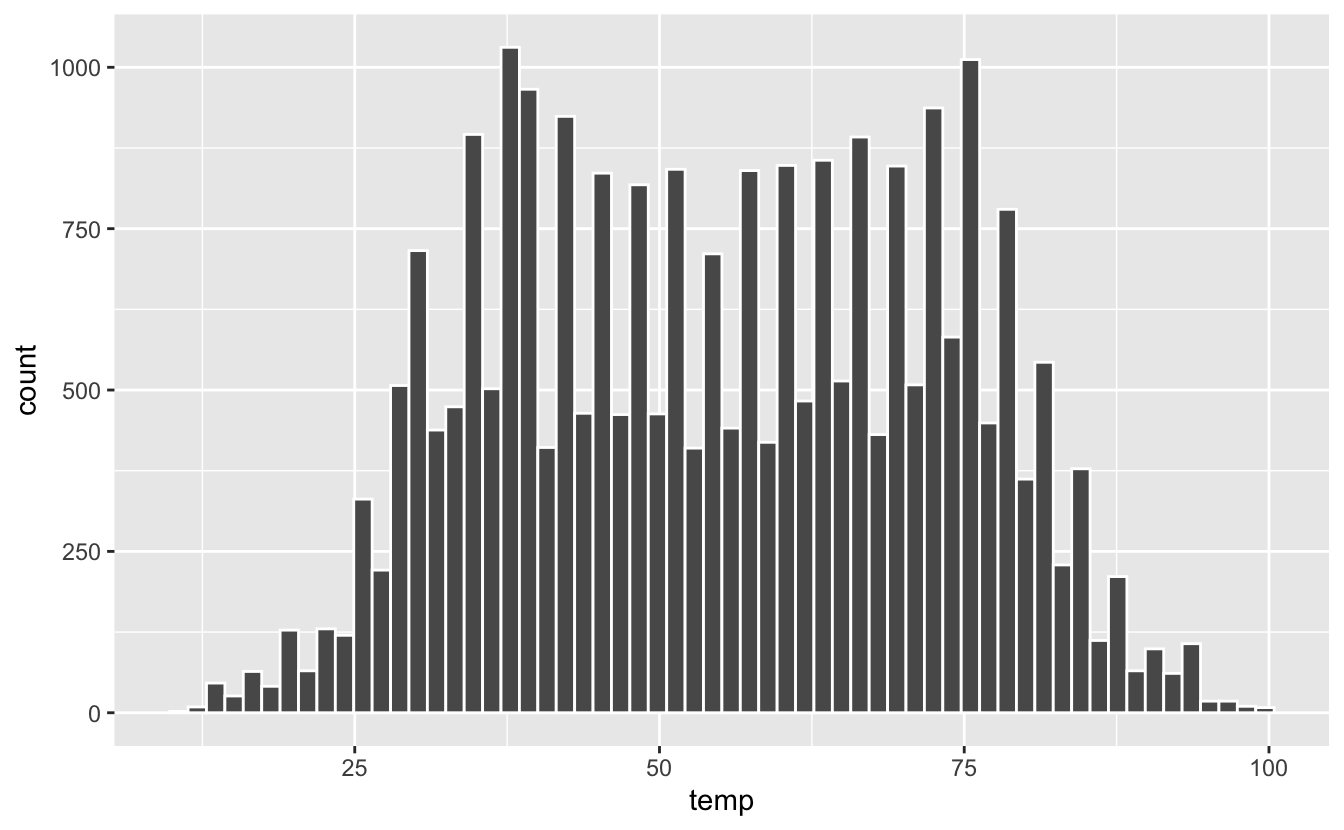
\includegraphics[width=0.9\linewidth]{figure/unnamed-chunk-49-1} 

}

\caption{Modification du nombre de classes.}\label{fig:unnamed-chunk-49}
\end{figure}

Ici, augmenter le nombre de classes à 60 permet de prendre conscience que la distribution n'est pas aussi lisse qu'elle en avait l'air. L'ajout d'une couche supplémentaire avec la fonction \texttt{geom\_rug()} (``a rug'' est un tapis en français) permet de prendre conscience que les données de température ne sont pas aussi continues qu'on pouvait le croire (figure \ref{fig:rughist}) :

\begin{Shaded}
\begin{Highlighting}[]
\KeywordTok{ggplot}\NormalTok{(weather, }\KeywordTok{aes}\NormalTok{(}\DataTypeTok{x =}\NormalTok{ temp)) }\OperatorTok{+}
\StringTok{  }\KeywordTok{geom_histogram}\NormalTok{(}\DataTypeTok{bins =} \DecValTok{60}\NormalTok{, }\DataTypeTok{color =} \StringTok{"white"}\NormalTok{) }\OperatorTok{+}
\StringTok{  }\KeywordTok{geom_rug}\NormalTok{(}\DataTypeTok{alpha =} \FloatTok{0.1}\NormalTok{)}
\end{Highlighting}
\end{Shaded}

\begin{figure}[htpb]

{\centering 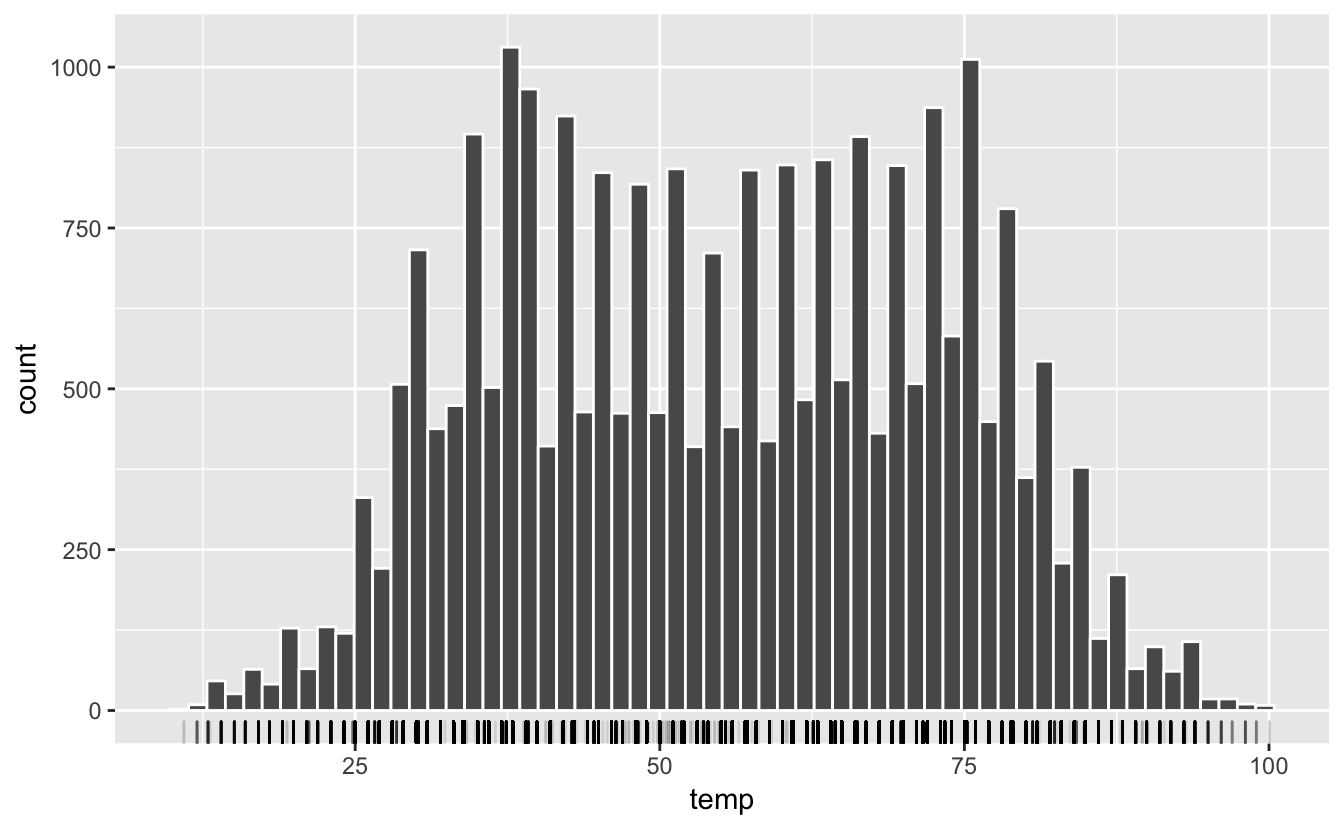
\includegraphics[width=0.9\linewidth]{figure/rughist-1} 

}

\caption{Ajout des données brutes sous forme de 'tapis' (`rug`) sous l'histogramme.}\label{fig:rughist}
\end{figure}

Notez la transparence importante utilisée pour \texttt{geom\_rug()}. On constate que la précision des relevés de température n'est en fait que de quelques dixièmes de degrés.

On peut également modifier la largeur des classes avec \texttt{binwidth} :

\begin{Shaded}
\begin{Highlighting}[]
\KeywordTok{ggplot}\NormalTok{(weather, }\KeywordTok{aes}\NormalTok{(}\DataTypeTok{x =}\NormalTok{ temp)) }\OperatorTok{+}
\StringTok{  }\KeywordTok{geom_histogram}\NormalTok{(}\DataTypeTok{binwidth =} \DecValTok{10}\NormalTok{, }\DataTypeTok{color =} \StringTok{"white"}\NormalTok{)}
\end{Highlighting}
\end{Shaded}

\begin{figure}[htpb]

{\centering 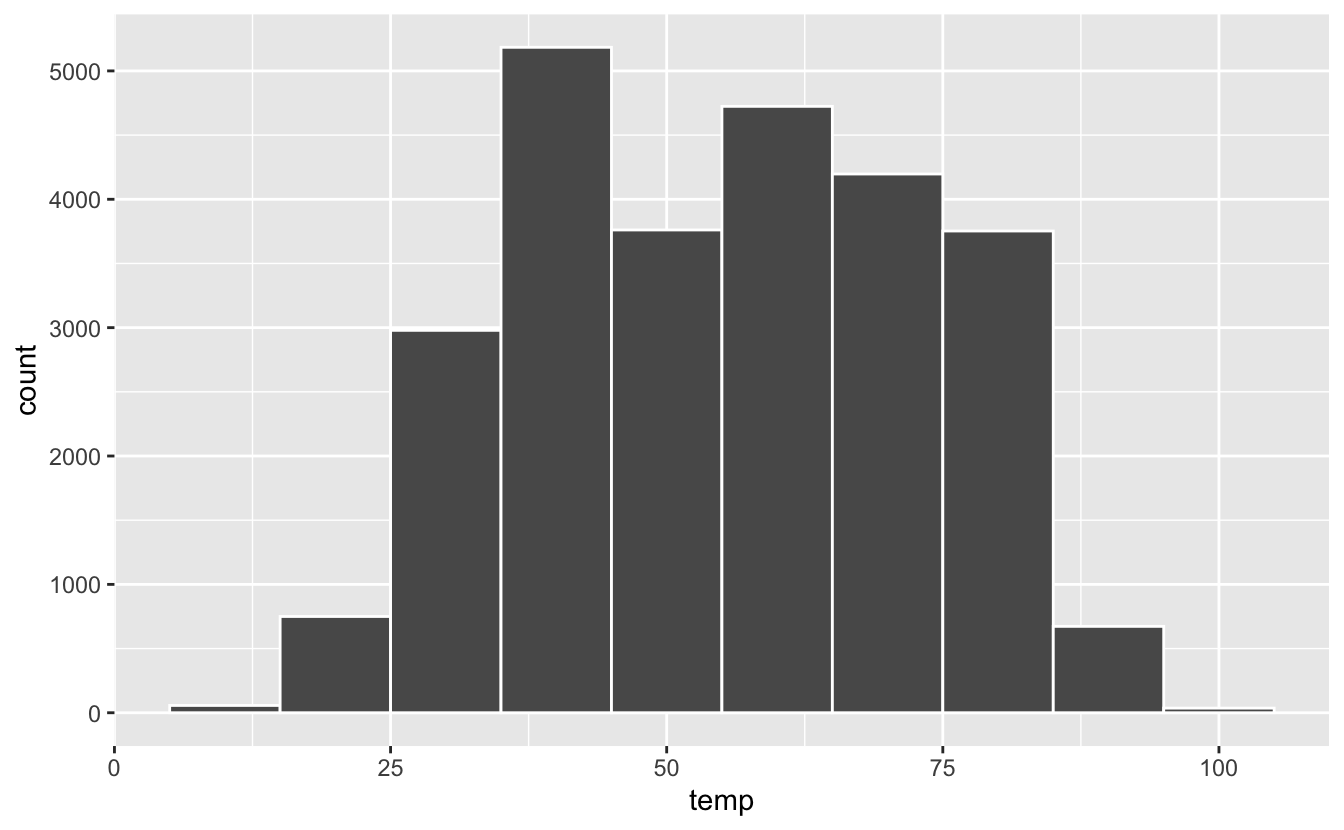
\includegraphics[width=0.9\linewidth]{figure/unnamed-chunk-50-1} 

}

\caption{Modification de la largeur des classes avec `binwidth`.}\label{fig:unnamed-chunk-50}
\end{figure}

Ici, chaque catégorie recouvre 10 degrés Farenheit, ce qui est probablement trop large puisque la bimodalité de la distribution est devenue presque invisible.

Enfin, il est possible de déterminer manuellement les limites des classes souhaitées avec l'argument \texttt{breaks} (figure \ref{fig:irregclasses}) :

\begin{Shaded}
\begin{Highlighting}[]
\KeywordTok{ggplot}\NormalTok{(weather, }\KeywordTok{aes}\NormalTok{(}\DataTypeTok{x =}\NormalTok{ temp)) }\OperatorTok{+}
\StringTok{  }\KeywordTok{geom_histogram}\NormalTok{(}\DataTypeTok{breaks =} \KeywordTok{c}\NormalTok{(}\DecValTok{0}\NormalTok{, }\DecValTok{10}\NormalTok{, }\DecValTok{20}\NormalTok{, }\DecValTok{50}\NormalTok{, }\DecValTok{60}\NormalTok{, }\DecValTok{70}\NormalTok{, }\DecValTok{80}\NormalTok{, }\DecValTok{105}\NormalTok{), }\DataTypeTok{color =} \StringTok{"white"}\NormalTok{)}
\end{Highlighting}
\end{Shaded}

\begin{figure}[htpb]

{\centering 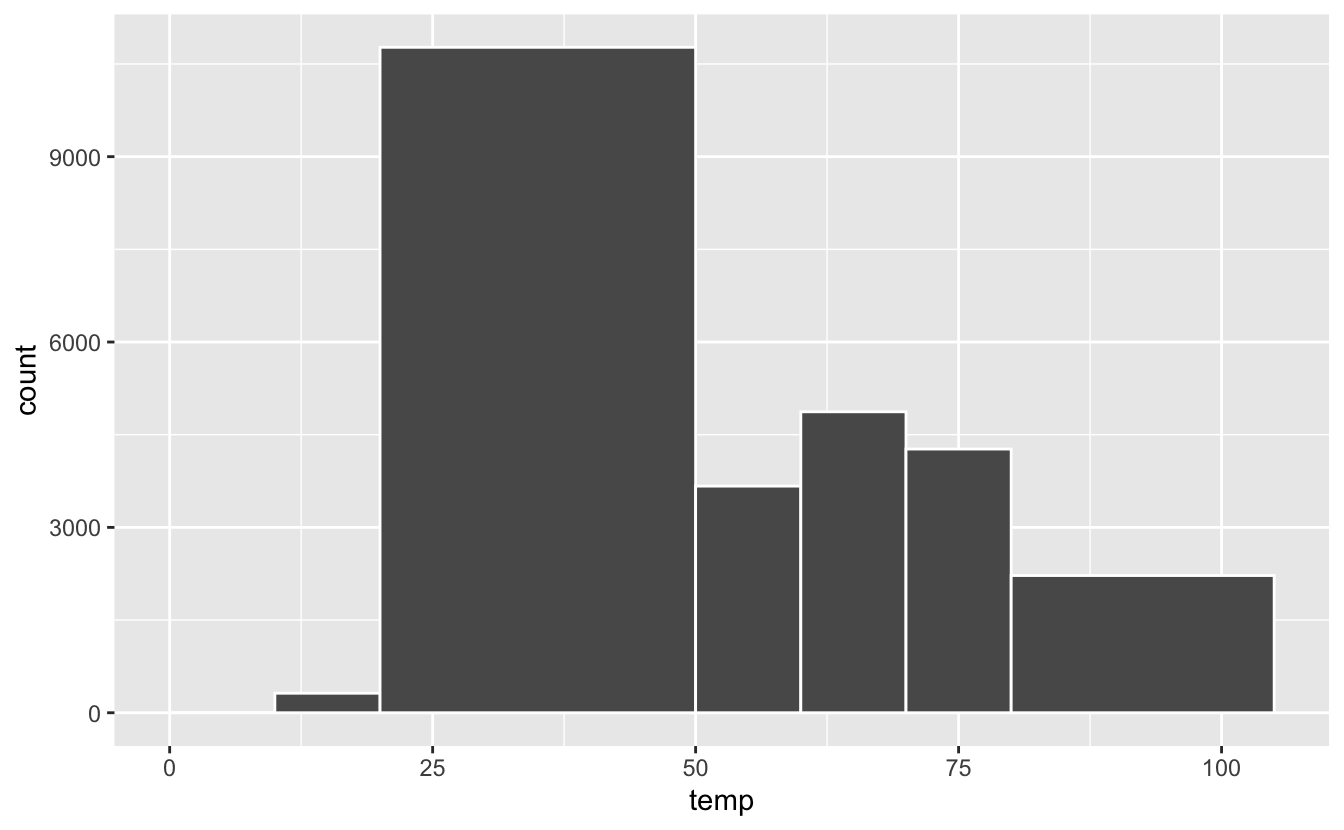
\includegraphics[width=0.9\linewidth]{figure/irregclasses-1} 

}

\caption{Spécification manuelle des limites de classes de tailles (classes irrégulières).}\label{fig:irregclasses}
\end{figure}

Vous constatez ici que les choix effectués ne sont pas très pertinents : toutes les classes n'ont pas la même largeur. Cela rend l'interprétation difficile. Il est donc vivement conseillé, pour spécifier \texttt{breaks}, de créer des suites régulières, comme avec la fonction \texttt{seq()} (consultez son fichier d'aide et les exemples) :

\begin{Shaded}
\begin{Highlighting}[]
\NormalTok{limits <-}\StringTok{ }\KeywordTok{seq}\NormalTok{(}\DataTypeTok{from =} \DecValTok{10}\NormalTok{, }\DataTypeTok{to =} \DecValTok{105}\NormalTok{, }\DataTypeTok{by =} \DecValTok{5}\NormalTok{)}
\NormalTok{limits}
\end{Highlighting}
\end{Shaded}

\begin{verbatim}
 [1]  10  15  20  25  30  35  40  45  50  55  60  65  70  75  80  85
[17]  90  95 100 105
\end{verbatim}

\begin{Shaded}
\begin{Highlighting}[]
\KeywordTok{ggplot}\NormalTok{(weather, }\KeywordTok{aes}\NormalTok{(}\DataTypeTok{x =}\NormalTok{ temp)) }\OperatorTok{+}
\StringTok{  }\KeywordTok{geom_histogram}\NormalTok{(}\DataTypeTok{breaks =}\NormalTok{ limits, }\DataTypeTok{color =} \StringTok{"white"}\NormalTok{)}
\end{Highlighting}
\end{Shaded}

\begin{figure}[htpb]

{\centering 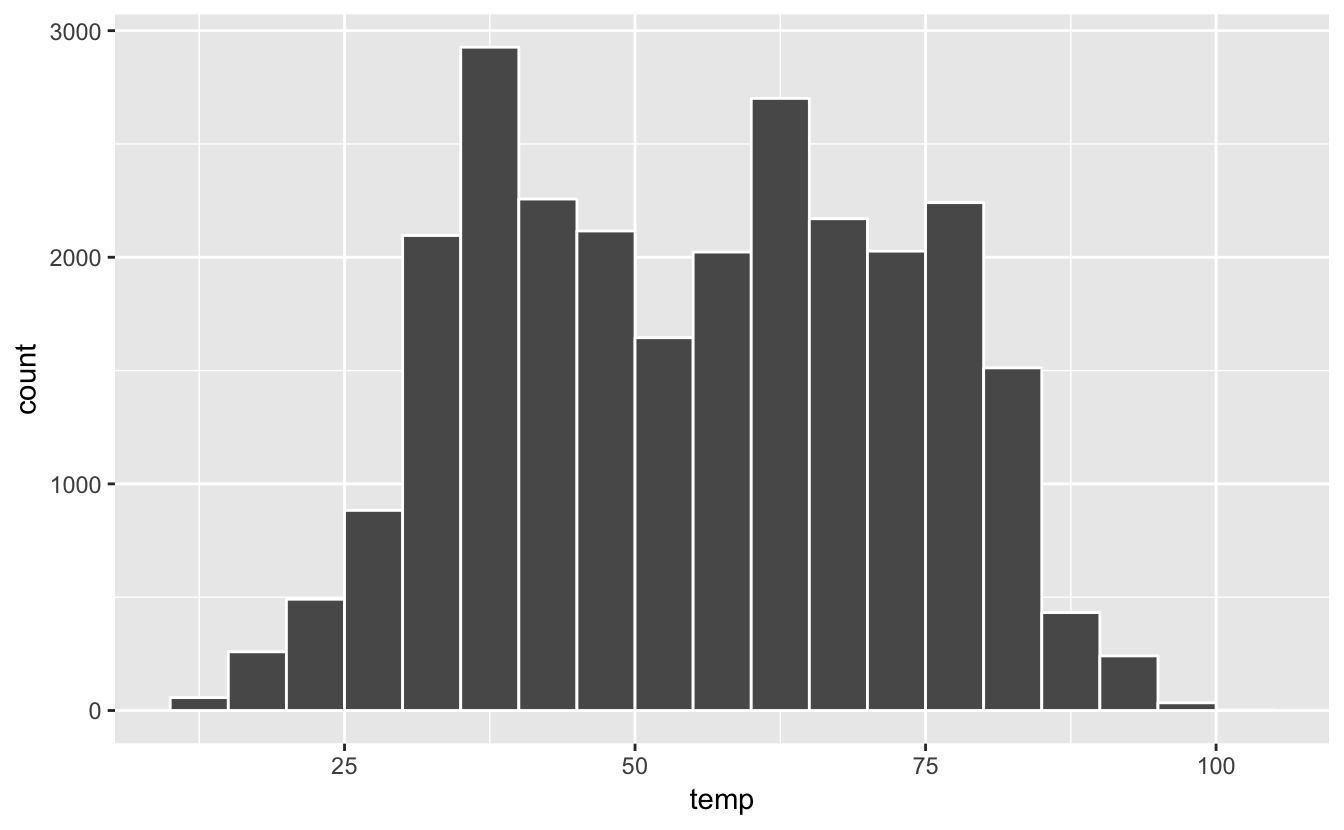
\includegraphics[width=0.9\linewidth]{figure/break-1} 

}

\caption{Un exemple d'utilisation de l'argument `breaks`.}\label{fig:break}
\end{figure}

Il est important que toute la gamme des valeurs de \texttt{temp} soit couverte par les limites des classes que nous avons définies, sinon, certaines valeurs sont omises et l'histogramme est donc incomplet/incorrect. Une façon de s'en assurer est d'afficher le résumé des données pour la colonne \texttt{temp} du jeu de données \texttt{weather} :

\begin{Shaded}
\begin{Highlighting}[]
\KeywordTok{summary}\NormalTok{(weather}\OperatorTok{$}\NormalTok{temp)}
\end{Highlighting}
\end{Shaded}

\begin{verbatim}
   Min. 1st Qu.  Median    Mean 3rd Qu.    Max.    NA's 
  10.94   39.92   55.40   55.26   69.98  100.04       1 
\end{verbatim}

On voit ici que les températures varient de 10.94 à 100.04 degrés Farenheit. Les classes que nous avons définies couvrent une plage de températures plus large (de 10 à 105). Toutes les données sont donc bien intégrées à l'histogramme.

\hypertarget{les-densituxe9s}{%
\subsubsection{Les densités}\label{les-densituxe9s}}

Une façon de s'affranchir (presque) complètement de cette question de largeur des classes de tailles et de représenter les distributions sous forme de courbes de densités :

\begin{Shaded}
\begin{Highlighting}[]
\KeywordTok{ggplot}\NormalTok{(weather, }\KeywordTok{aes}\NormalTok{(}\DataTypeTok{x =}\NormalTok{ temp)) }\OperatorTok{+}
\StringTok{  }\KeywordTok{geom_density}\NormalTok{()}
\end{Highlighting}
\end{Shaded}

\begin{figure}[htpb]

{\centering 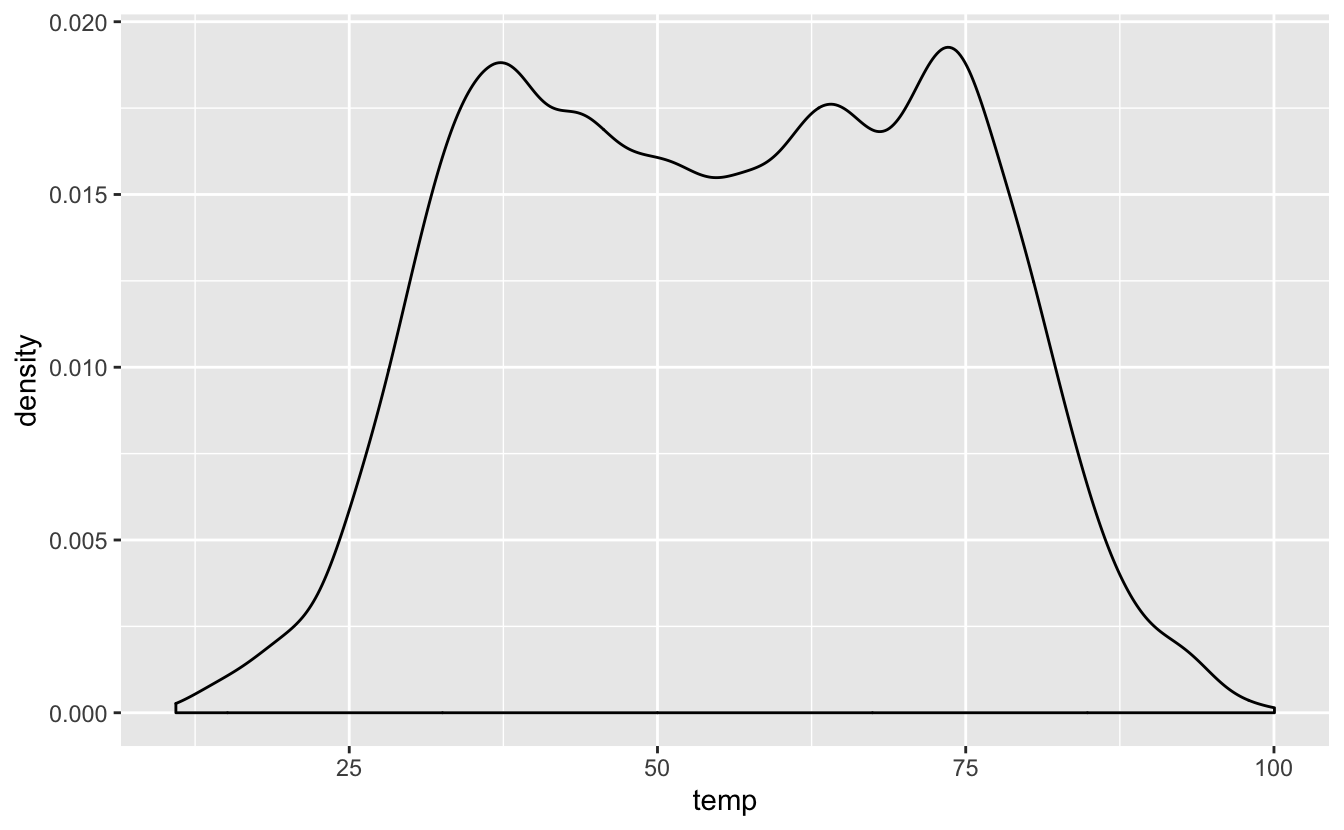
\includegraphics[width=0.9\linewidth]{figure/density-1} 

}

\caption{Un exemple de courbe de densité.}\label{fig:density}
\end{figure}

Ici, la courbe reflète non pas la fréquence des données dans des classes de tailles, mais leur densité, c'est à dire que la surface totale sous la courbe vaut 1 (d'où l'échelle étrange sur l'axe des ordonnées). C'est une extention continue de l'histogramme par nature discontinu. On repère bien ici les 2 pics identifiés précédemments qui correspondent à des densités de données plus fortes pour les températures de 30 et 70 degrés Farenheit environ.
La courbe possède un paramètre de lissage (\texttt{bw} pour ``bandwidth'') qui équivaut un peu à la largeur des classes de taille d'un histogramme :

\begin{Shaded}
\begin{Highlighting}[]
\KeywordTok{ggplot}\NormalTok{(weather, }\KeywordTok{aes}\NormalTok{(}\DataTypeTok{x =}\NormalTok{ temp)) }\OperatorTok{+}
\StringTok{  }\KeywordTok{geom_density}\NormalTok{(}\DataTypeTok{bw =} \FloatTok{0.5}\NormalTok{)}
\end{Highlighting}
\end{Shaded}

\begin{figure}[htpb]

{\centering 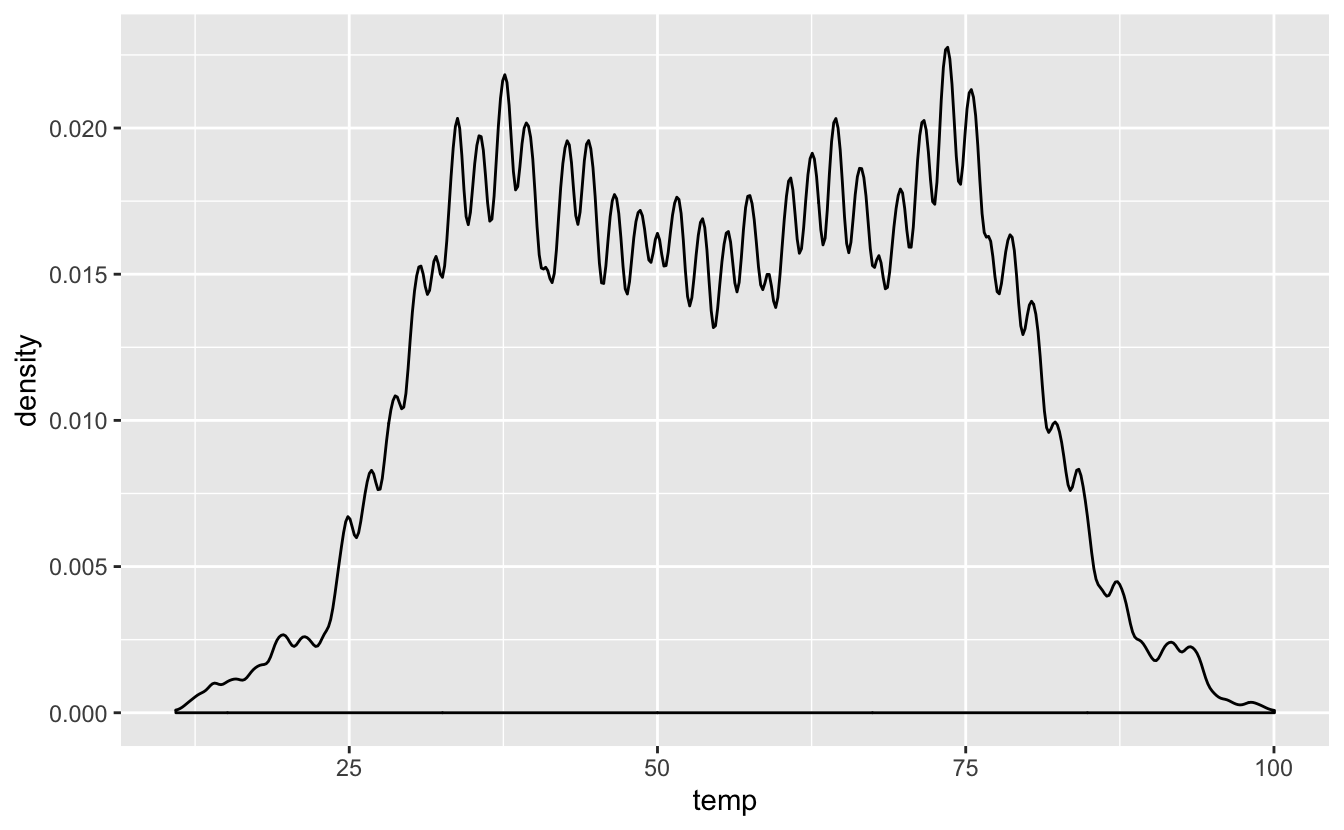
\includegraphics[width=0.9\linewidth]{figure/densitynarrow-1} 

}

\caption{Un exemple de courbe de densité trop peu lissée.}\label{fig:densitynarrow}
\end{figure}

Ici, les données sont trop peu lissées et la courbe est donc très ``bruitée''.

\begin{Shaded}
\begin{Highlighting}[]
\KeywordTok{ggplot}\NormalTok{(weather, }\KeywordTok{aes}\NormalTok{(}\DataTypeTok{x =}\NormalTok{ temp)) }\OperatorTok{+}
\StringTok{  }\KeywordTok{geom_density}\NormalTok{(}\DataTypeTok{bw =} \DecValTok{10}\NormalTok{)}
\end{Highlighting}
\end{Shaded}

\begin{figure}[htpb]

{\centering 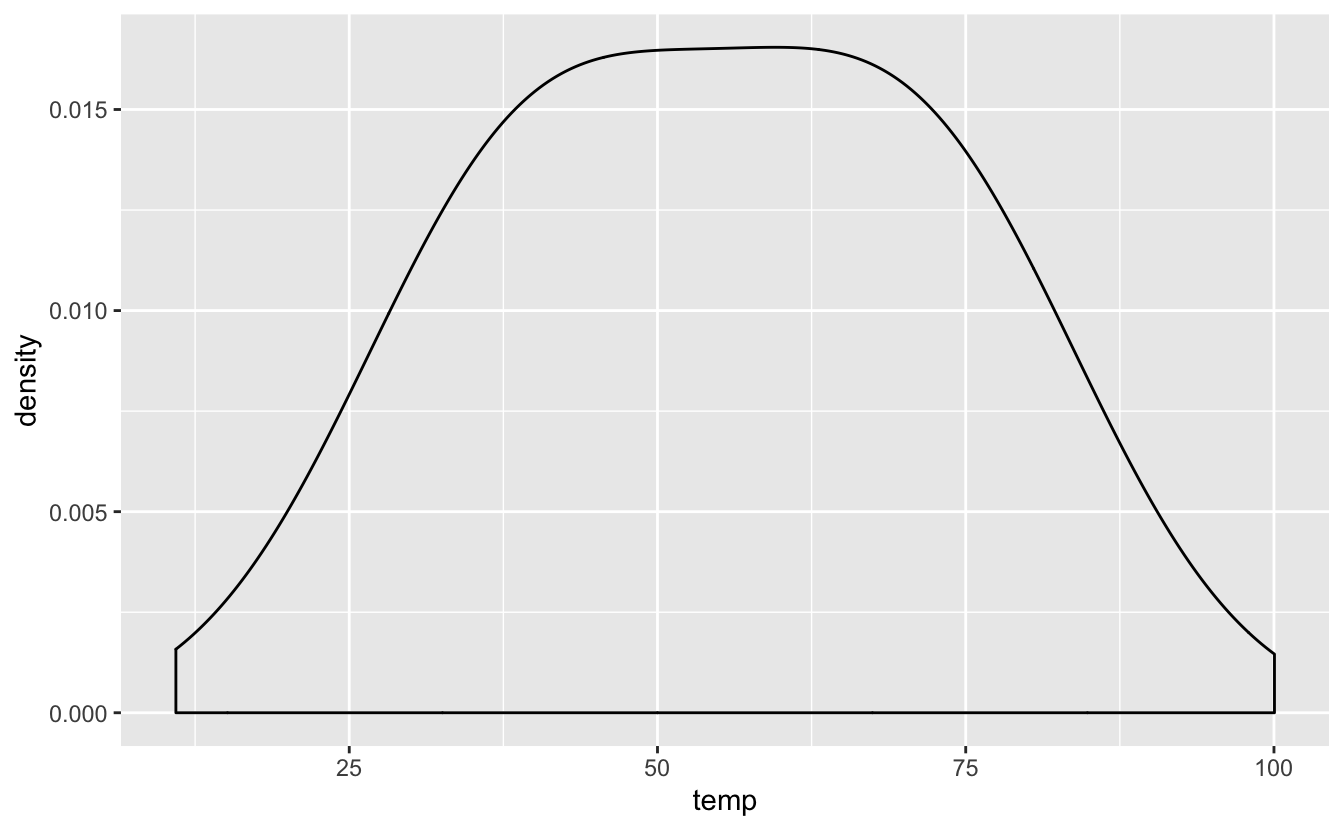
\includegraphics[width=0.9\linewidth]{figure/densitywide-1} 

}

\caption{Un exemple de courbe de densité trop lissée.}\label{fig:densitywide}
\end{figure}

Ici, la courbe est trop lissée donc toute la structure des données disparaît. En règle générale, la valeur choisie par défaut par \texttt{geom\_density()} pour le paramètre \texttt{bw} est tout à fait satisfaisante. Il est donc rare que l'utilisateur ait à modifier manuellement cette valeur.

\begin{center}\rule{0.5\linewidth}{0.5pt}\end{center}

\hypertarget{facets}{%
\subsection{\texorpdfstring{Les \texttt{facet}s}{Les facets}}\label{facets}}

\hypertarget{facet_wrap}{%
\subsubsection{\texorpdfstring{\texttt{facet\_wrap()}}{facet\_wrap()}}\label{facet_wrap}}

Nous l'avons indiqué plus haut, les \texttt{facet}s permettent de scinder le jeu de données en plusieurs sous-groupes et de faire un graphique pour chacun des sous-groupes.

Ainsi, si l'on souhaite connaître la distribution des températures pour chaque mois de l'année 2013, plutôt que de faire ceci :

\begin{Shaded}
\begin{Highlighting}[]
\KeywordTok{ggplot}\NormalTok{(weather, }\KeywordTok{aes}\NormalTok{(}\DataTypeTok{x =}\NormalTok{ temp, }\DataTypeTok{fill =} \KeywordTok{factor}\NormalTok{(month))) }\OperatorTok{+}
\StringTok{  }\KeywordTok{geom_histogram}\NormalTok{(}\DataTypeTok{bins =} \DecValTok{20}\NormalTok{, }\DataTypeTok{color =} \StringTok{"grey30"}\NormalTok{)}
\end{Highlighting}
\end{Shaded}

\begin{figure}[htpb]

{\centering 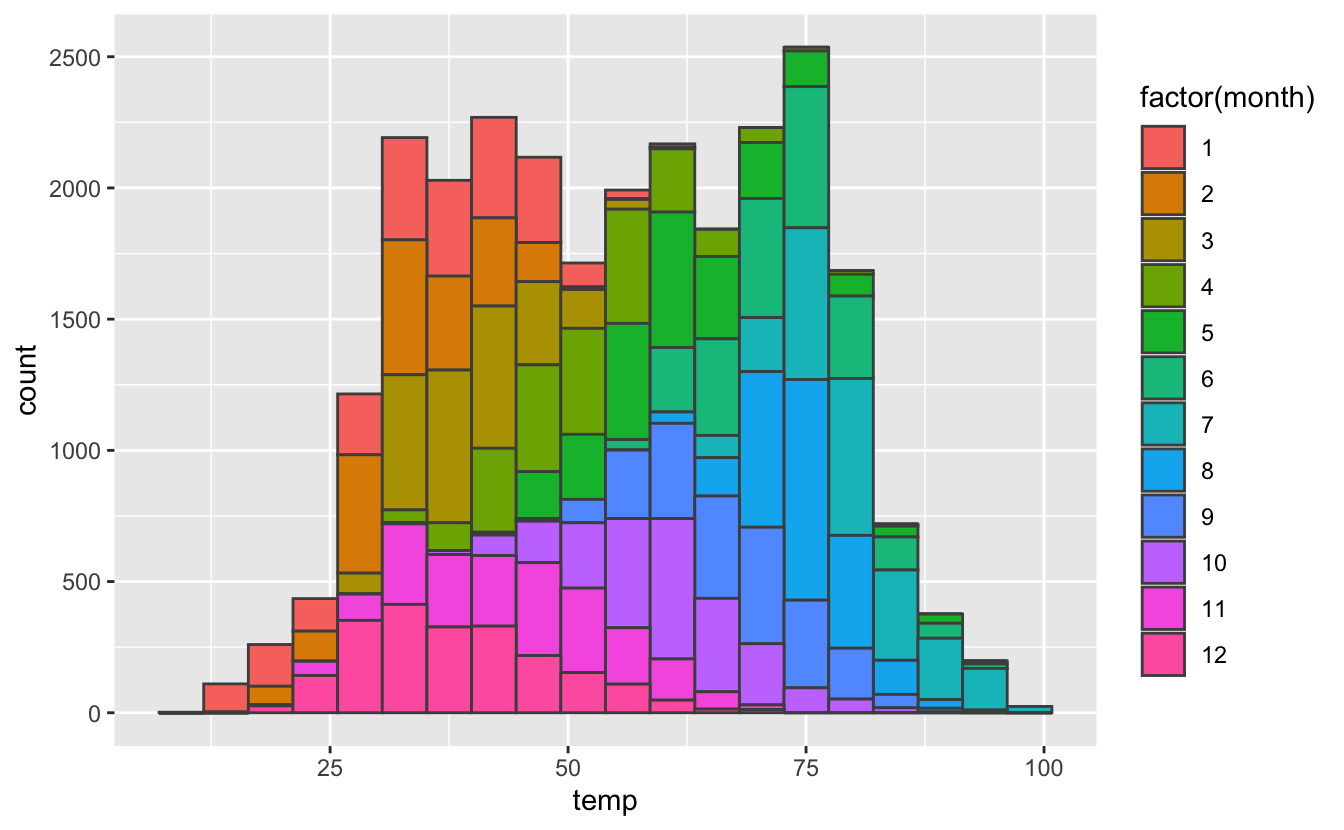
\includegraphics[width=0.9\linewidth]{figure/unnamed-chunk-52-1} 

}

\caption{Distribution des températures avec visualisation des données mensuelles.}\label{fig:unnamed-chunk-52}
\end{figure}

qui produit un graphique certes assez joli, mais difficile à interpréter, mieux vaut faire ceci :

\begin{Shaded}
\begin{Highlighting}[]
\KeywordTok{ggplot}\NormalTok{(weather, }\KeywordTok{aes}\NormalTok{(}\DataTypeTok{x =}\NormalTok{ temp, }\DataTypeTok{fill =} \KeywordTok{factor}\NormalTok{(month))) }\OperatorTok{+}
\StringTok{  }\KeywordTok{geom_histogram}\NormalTok{(}\DataTypeTok{bins =} \DecValTok{20}\NormalTok{, }\DataTypeTok{color =} \StringTok{"grey30"}\NormalTok{) }\OperatorTok{+}
\StringTok{  }\KeywordTok{facet_wrap}\NormalTok{(}\OperatorTok{~}\KeywordTok{factor}\NormalTok{(month), }\DataTypeTok{ncol =} \DecValTok{3}\NormalTok{)}
\end{Highlighting}
\end{Shaded}

\begin{figure}[htpb]

{\centering 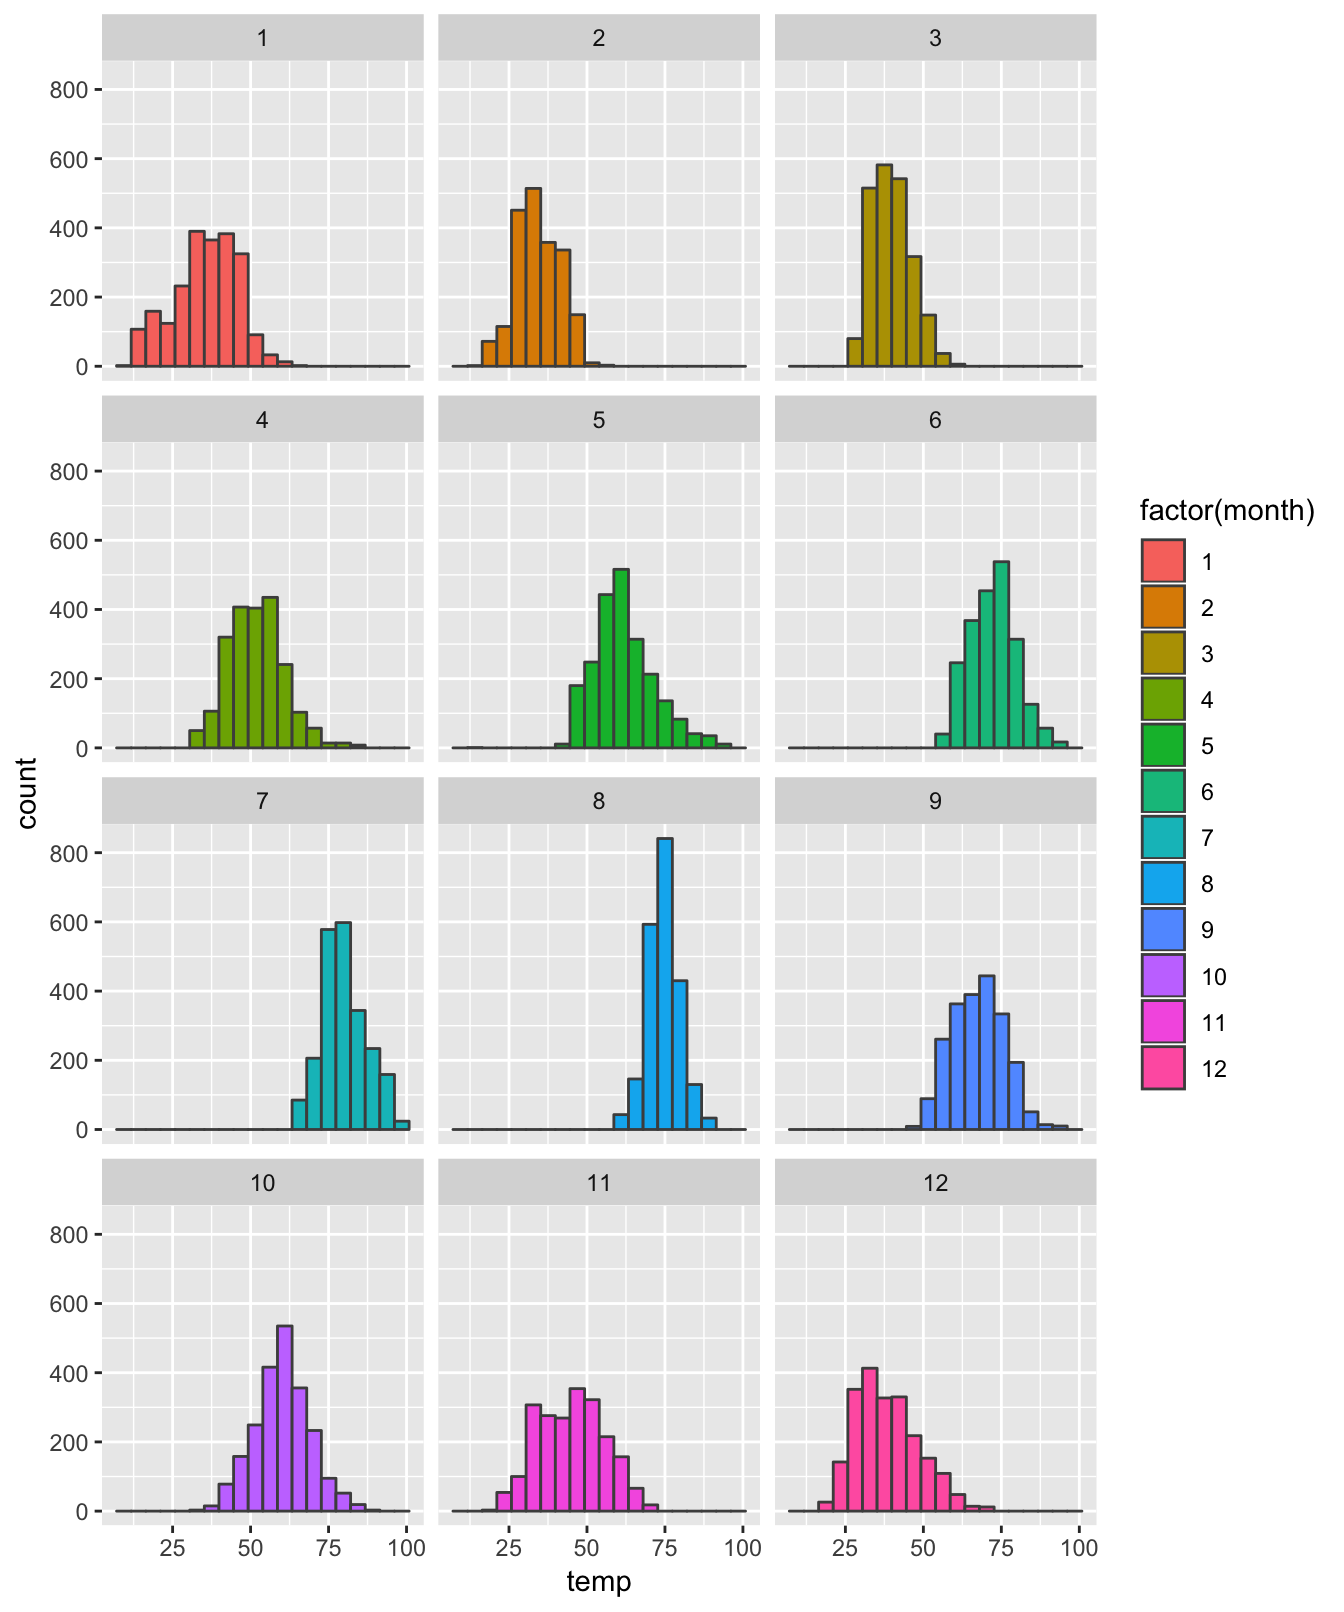
\includegraphics[width=0.9\linewidth]{figure/wrap-1} 

}

\caption{Un exemple d'utilisation de \texttt{facet\_wrap()}.}\label{fig:wrap}
\end{figure}



La couche supplémentaire créée avec \texttt{facet\_wrap()} permet donc de scinder les données en fonction d'une variable. Attention à la syntaxe : il ne faut pas oublier le symbole ``\texttt{\textasciitilde{}}'' devant la variable que l'on souhaite utiliser pour scinder les données. Il va sans dire que la variable utilisée doit être catégorielle et non continue, c'est la raison pour laquelle j'utilise la notation \texttt{factor(month)} et non simplement \texttt{month}.

Avec la fonction \texttt{facet\_wrap()}, il est possible d'indiquer à R comment les différents graphiques doivent être agencés en spécifiant soit le nombre de colonnes souhaité avec \texttt{ncol}, soit le nombre de lignes souhaité avec \texttt{nrow}.

\hypertarget{facet_grid}{%
\subsubsection{\texorpdfstring{\texttt{facet\_grid()}}{facet\_grid()}}\label{facet_grid}}

Une autre fonction nommée \texttt{facet\_grid()} permet d'agencer des sous-graphiques selon 2 variables catégorielles. Par exemple :

\begin{Shaded}
\begin{Highlighting}[]
\KeywordTok{ggplot}\NormalTok{(weather, }\KeywordTok{aes}\NormalTok{(}\DataTypeTok{x =}\NormalTok{ temp, }\DataTypeTok{fill =} \KeywordTok{factor}\NormalTok{(month))) }\OperatorTok{+}
\StringTok{  }\KeywordTok{geom_histogram}\NormalTok{(}\DataTypeTok{bins =} \DecValTok{20}\NormalTok{, }\DataTypeTok{color =} \StringTok{"grey30"}\NormalTok{) }\OperatorTok{+}
\StringTok{  }\KeywordTok{facet_grid}\NormalTok{(}\KeywordTok{factor}\NormalTok{(month) }\OperatorTok{~}\StringTok{ }\NormalTok{origin)}
\end{Highlighting}
\end{Shaded}

\begin{figure}[htpb]

{\centering 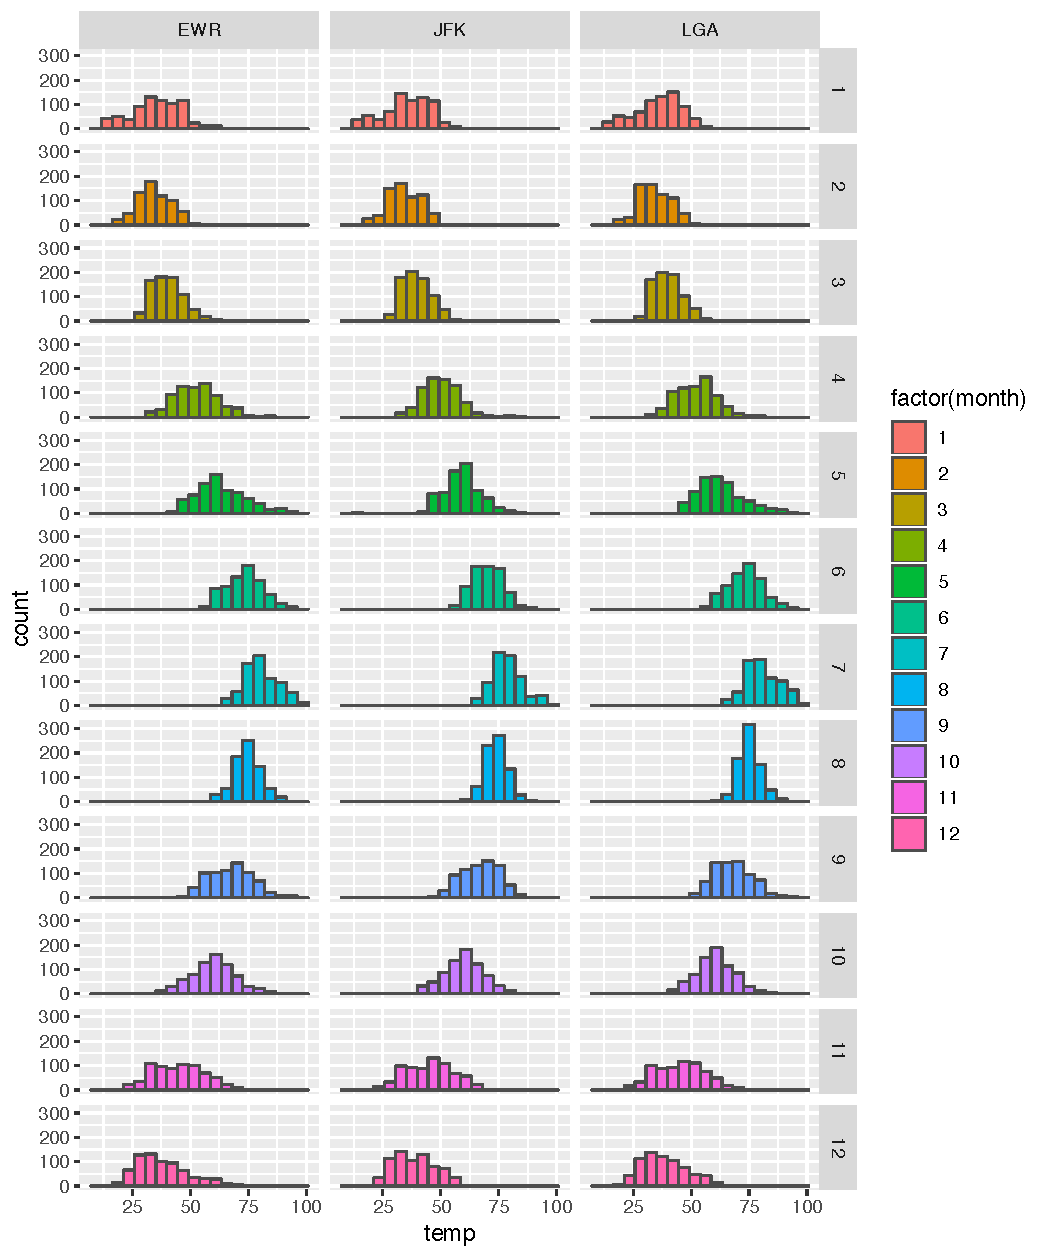
\includegraphics[width=0.9\linewidth]{figure/grid-1} 

}

\caption{Un exemple d'utilisation de \texttt{facet\_grid()}.}\label{fig:grid}
\end{figure}



Ici, nous avons utilisé la variable \texttt{month} (transformée en facteur) et la variable \texttt{origin} pour créer un histogramme pour chaque combinaison des modalités de ces 2 variables. Il est donc possible de comparer facilement des températures inter-mensuelles au sein d'un aéroport donné (en colonnes), ou de comparer des températures enregistrées le même mois dans des aéroports distincts (en lignes).

\texttt{facet\_grid()} doit elle aussi être utilisée avec le symbole ``\texttt{\textasciitilde{}}''. Comme pour les indices d'un tableau, on met à gauche du ``\texttt{\textasciitilde{}}'' la variable qui figurera en lignes, et à droite du \texttt{\textasciitilde{}} celle qui figurera en colonnes. Les arguments \texttt{nrow} et \texttt{ncol} ne peuvent donc pas être utilisés : c'est le nombre de niveaux de chaque variable catégorielle fournie à \texttt{facet\_grid()} qui détermine le nombre de lignes et de colonnes du graphique.

Vous devriez maintenant être convaincus de la puissance de la grammaire des graphiques. En utilisant un langage standardisé et en ajoutant des couches une à une sur un graphique, il est posible d'obtenir rapidement des visualisations très complexes et néanmoins très claires, qui font apparaître des structures intéressantes dans nos données (des tendances, des groupes, des similitudes, des liaisons, des différences, etc.).

\hypertarget{exercices-4}{%
\subsubsection{Exercices}\label{exercices-4}}

Examinez la figure \ref{fig:grid}.

\begin{enumerate}
\def\labelenumi{\arabic{enumi}.}
\tightlist
\item
  Quels éléments nouveaux ce graphique nous apprend-il par rapport au graphique \ref{fig:break} ci-dessus ? Comment le ``\texttt{facet}ing'' nous aide-t'il à visualiser les relations entre 2 (ou 3) variables ?
\item
  À quoi correspondent les numéros 1 à 12 ?
\item
  À quoi correspondent les chiffres 25, 50, 75, 100 ?
\item
  À quoi correspondent les chiffres 0, 100, 200, 300 ?
\item
  Observez les échelles des axes \texttt{x} et \texttt{y} pour chaque sous graphique. Qu'ont-elles de particulier ? En quoi est-ce utile ?
\item
  La variabilité des températures est-elle plus importante entre les aéroports, entre les mois, ou au sein des mois ? Expliquez votre réflexion.
\end{enumerate}

\begin{center}\rule{0.5\linewidth}{0.5pt}\end{center}

\hypertarget{les-bouxeetes-uxe0-moustaches-ou-boxplots}{%
\subsection{Les boîtes à moustaches ou boxplots}\label{les-bouxeetes-uxe0-moustaches-ou-boxplots}}

\hypertarget{cruxe9ation-de-boxplots-et-informations-apportuxe9es}{%
\subsubsection{Création de boxplots et informations apportées}\label{cruxe9ation-de-boxplots-et-informations-apportuxe9es}}

Commençons par créer un boxplot pour comparer les températures mensuelles comme nous l'avons fait plus haut avec des histogrammes :

\begin{Shaded}
\begin{Highlighting}[]
\KeywordTok{ggplot}\NormalTok{(weather, }\KeywordTok{aes}\NormalTok{(}\DataTypeTok{x =}\NormalTok{ month, }\DataTypeTok{y =}\NormalTok{ temp)) }\OperatorTok{+}
\StringTok{  }\KeywordTok{geom_boxplot}\NormalTok{()}
\end{Highlighting}
\end{Shaded}

\begin{verbatim}
Warning: Continuous x aesthetic -- did you forget aes(group=...)?
\end{verbatim}

\begin{verbatim}
Warning: Removed 1 rows containing non-finite values (stat_boxplot).
\end{verbatim}

\begin{figure}[htpb]

{\centering 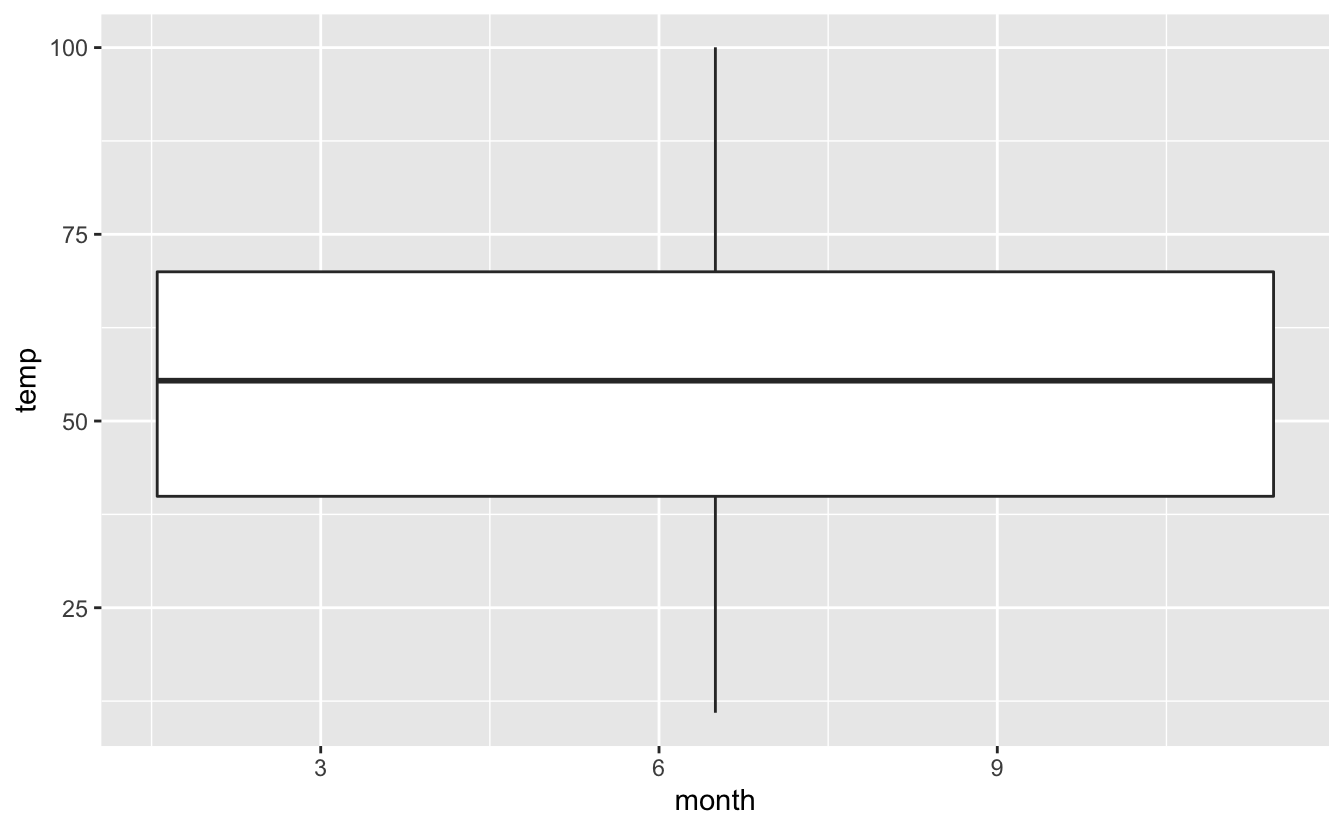
\includegraphics[width=0.9\linewidth]{figure/unnamed-chunk-53-1} 

}

\caption{Un boxplot fort peu utile...}\label{fig:unnamed-chunk-53}
\end{figure}

Comme précédemment, R nous avertit qu'une observation n'a pas été intégrée (en raison d'une donnée manquante). Mais il nous dit aussi que \texttt{x} (pour nous, la variable \texttt{month}) est continue, et que nous avons probablement oublié de spécifier des groupes.

En effet, les boxplots sont généralement utilisés pour examiner la distribution d'une variable numérique pour chaque niveau d'une variable catégorielle (un facteur). Il nous faut donc, ici encore, transformer \texttt{month} en facteur car dans notre tableau de départ, cette variable est considérée comme une variable numérique continue :

\begin{Shaded}
\begin{Highlighting}[]
\KeywordTok{ggplot}\NormalTok{(weather, }\KeywordTok{aes}\NormalTok{(}\DataTypeTok{x =} \KeywordTok{factor}\NormalTok{(month), }\DataTypeTok{y =}\NormalTok{ temp)) }\OperatorTok{+}
\StringTok{  }\KeywordTok{geom_boxplot}\NormalTok{()}
\end{Highlighting}
\end{Shaded}

\begin{figure}[htpb]

{\centering 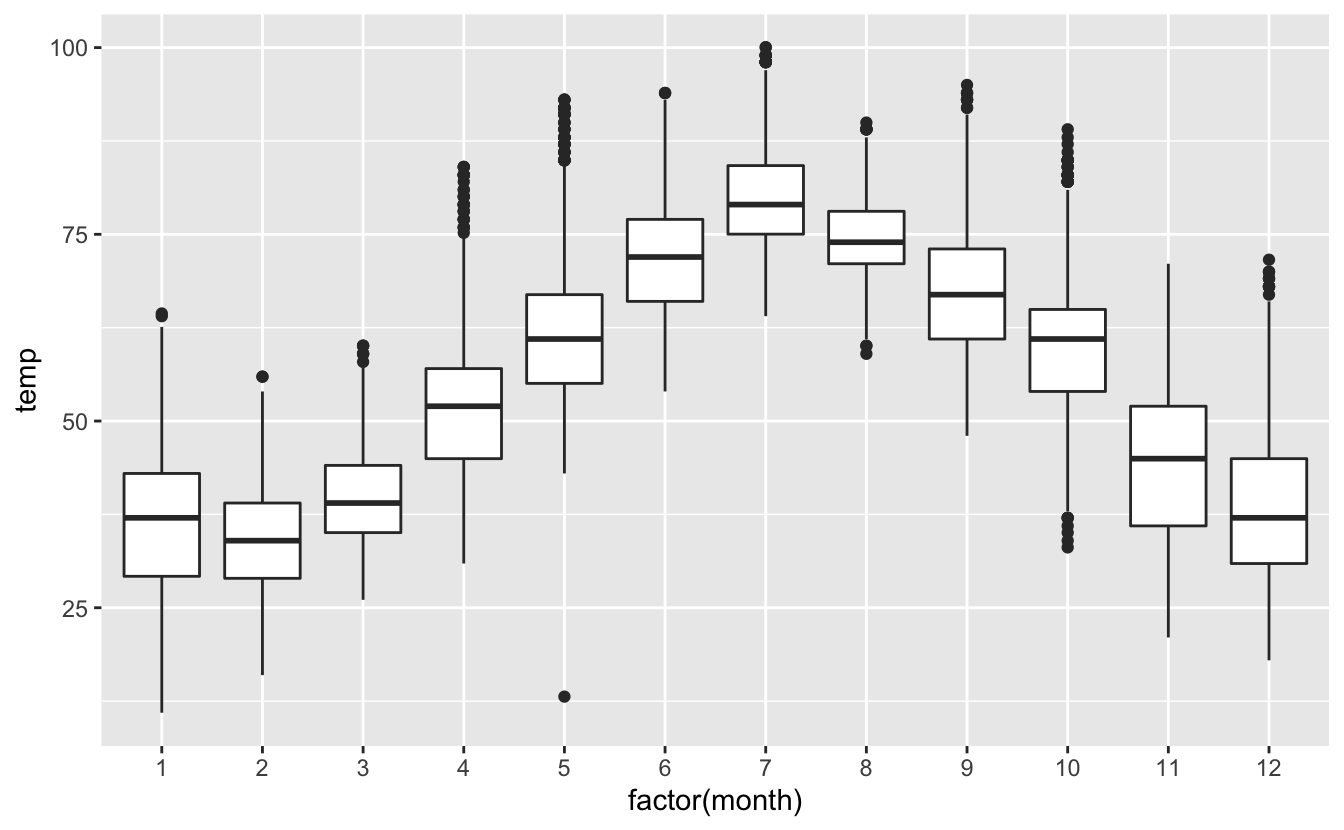
\includegraphics[width=0.9\linewidth]{figure/unnamed-chunk-54-1} 

}

\caption{Boxplot des températures mensuelles.}\label{fig:unnamed-chunk-54}
\end{figure}

Les différents éléments d'un boxplot, sont les suivants :

\begin{itemize}
\tightlist
\item
  La limite inférieure de la boîte correspond au premier quartile : 25\% des données de l'échantillon sont situées au-dessous de cette valeur.
\item
  La limite supérieure de la boîte correspond au troisième quartile : 25\% des données de l'échantillon sont situées au-dessus de cette valeur.
\item
  Le segment épais à l'intérieur de la boîte correspond au second quartile : c'est la médiane de l'échantillon. 50\% des données de l'échantillon sont situées au-dessus de cette valeur, et 50\% au-dessous.
\item
  La hauteur de la boîte correspond à ce que l'on appelle l'étendue inter-quartile ou Inter Quartile Range (IQR) en anglais. On trouve dans cette boîte 50\% des observations de l'échantillon. C'est une mesure de la dispersion des 50\% des données les plus centrales. Une boîte plus allongée indique donc une plus grande dispersion.
\item
  Les moustaches correspondent à des valeurs qui sont en dessous du premier quartile (pour la moustache du bas) et au-dessus du troisième quartile (pour la moustache du haut). La règle utilisée dans R est que ces moustaches s'étendent jusqu'aux valeurs minimales et maximales de l'échantillon, mais elles ne peuvent en aucun cas s'étendre au-delà de 1,5 fois la hauteur de la boîte (1,5 fois l'IQR) vers le haut et le bas. Si des points apparaissent au-delà des moustaches (vers le haut ou le bas), ces points sont appelés ``outliers''. Ce sont des points qui s'éloignent du centre de la distribution de façon importante puisqu'ils sont au-delà de 1,5 fois l'IQR de part et d'autre du premier ou du troisième quartile. Il peut s'agir d'anomalies de mesures, d'anomalies de saisie des données, ou tout simplement, d'enregistrements tout à fait valides mais extrêmes. J'attire votre attention sur le fait que la définition de ces outliers est relativement arbitraire. Nous pourrions faire le choix d'étendre les moustaches jusqu'à 1,8 fois l'IQR (ou 2, ou 2,5). Nous observerions alors beaucoup moins d'outliers. D'une façons générale, la longueur des moustaches renseigne sur la variabilité des données en dehors de la zone centrale. Plus elles sont longues, plus la variabilité est importante. Et dans tous les cas, l'examen attentif des outliers est utile car il nous permet d'en apprendre plus sur le comportement extrême de certaines observations.
\end{itemize}

\hypertarget{lintervalle-de-confiance-uxe0-95-de-la-muxe9diane}{%
\subsubsection{L'intervalle de confiance à 95\% de la médiane}\label{lintervalle-de-confiance-uxe0-95-de-la-muxe9diane}}

On peut également aujouter une encoche autour de la valeur de médiane en ajoutant l'argument \texttt{notch\ =\ TRUE} à la fonction \texttt{geom\_boxplot()} :

\begin{Shaded}
\begin{Highlighting}[]
\KeywordTok{ggplot}\NormalTok{(weather, }\KeywordTok{aes}\NormalTok{(}\DataTypeTok{x =} \KeywordTok{factor}\NormalTok{(month), }\DataTypeTok{y =}\NormalTok{ temp)) }\OperatorTok{+}
\StringTok{  }\KeywordTok{geom_boxplot}\NormalTok{(}\DataTypeTok{notch =} \OtherTok{TRUE}\NormalTok{)}
\end{Highlighting}
\end{Shaded}

\begin{figure}[htpb]

{\centering 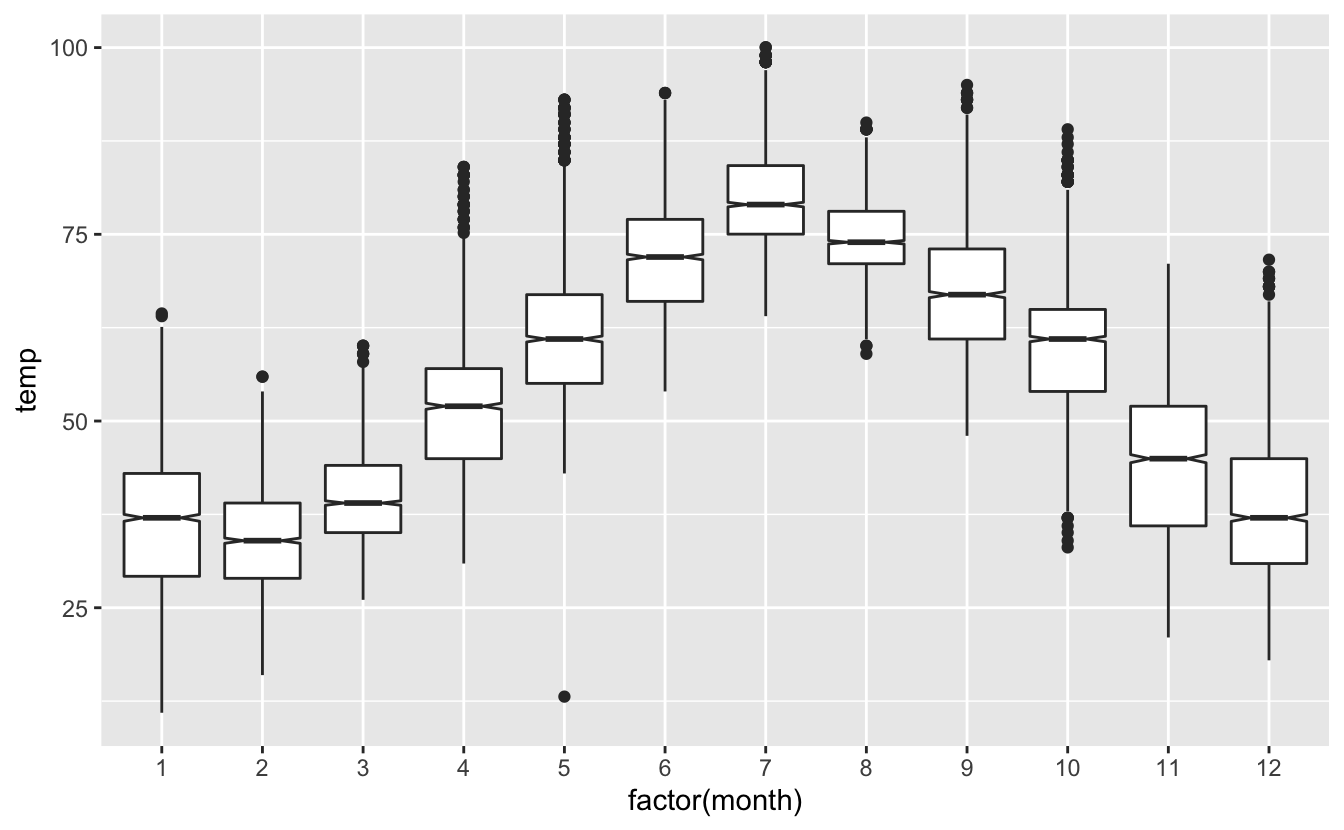
\includegraphics[width=0.9\linewidth]{figure/notchedboxplot-1} 

}

\caption{Boxplot des températures mensuelles. Les intervalles de confiance à 95\% de la médiane sont affichés.}\label{fig:notchedboxplot}
\end{figure}



Comme l'indique la légende de la figure \ref{fig:notchedboxplot}, cette encoche correspond à l'étendue de l'intervalle de confiance à 95\% de la médiane. Pour chaque échantillon, nous espérons que la médiane calculée soit le reflet fidèle de la vraie valeur de médiane de la population. Mais il sera toujours impossible d'en avoir la certitude absolue. Le mieux que l'on puisse faire, c'est quantifier l'incertitude. L'intervalle de confiance nous indique qu'il y a de bonnes chances que la vraie valeur de médiane de la population générale (qui restera à jamais inconnue) se trouve dans cet intervalle. Ici, les encoches sont très étroites car les données sont abondantes. Il y a donc peu d'incertitude, ce qui est une bonne chose. Cette notion d'intervalle de confiance est importante et ce type de graphique nous permettra d'anticiper sur les résultats des tests de comparaisons de moyennes.

\hypertarget{une-autre-fauxe7on-dexaminer-des-distributions}{%
\subsubsection{Une autre façon d'examiner des distributions}\label{une-autre-fauxe7on-dexaminer-des-distributions}}

Dernière chose concernant les boxplots : il s'agit d'une représentation graphique très proche de l'histogramme. Pour vous en convaincre, je représente à la figure \ref{fig:compboxplot} ci-dessous uniquement les températures du mois de novembre, avec 3 types d'objets géométriques différents : un histogramme, un boxplot, et un nuage de points.

\begin{figure}[htpb]

{\centering 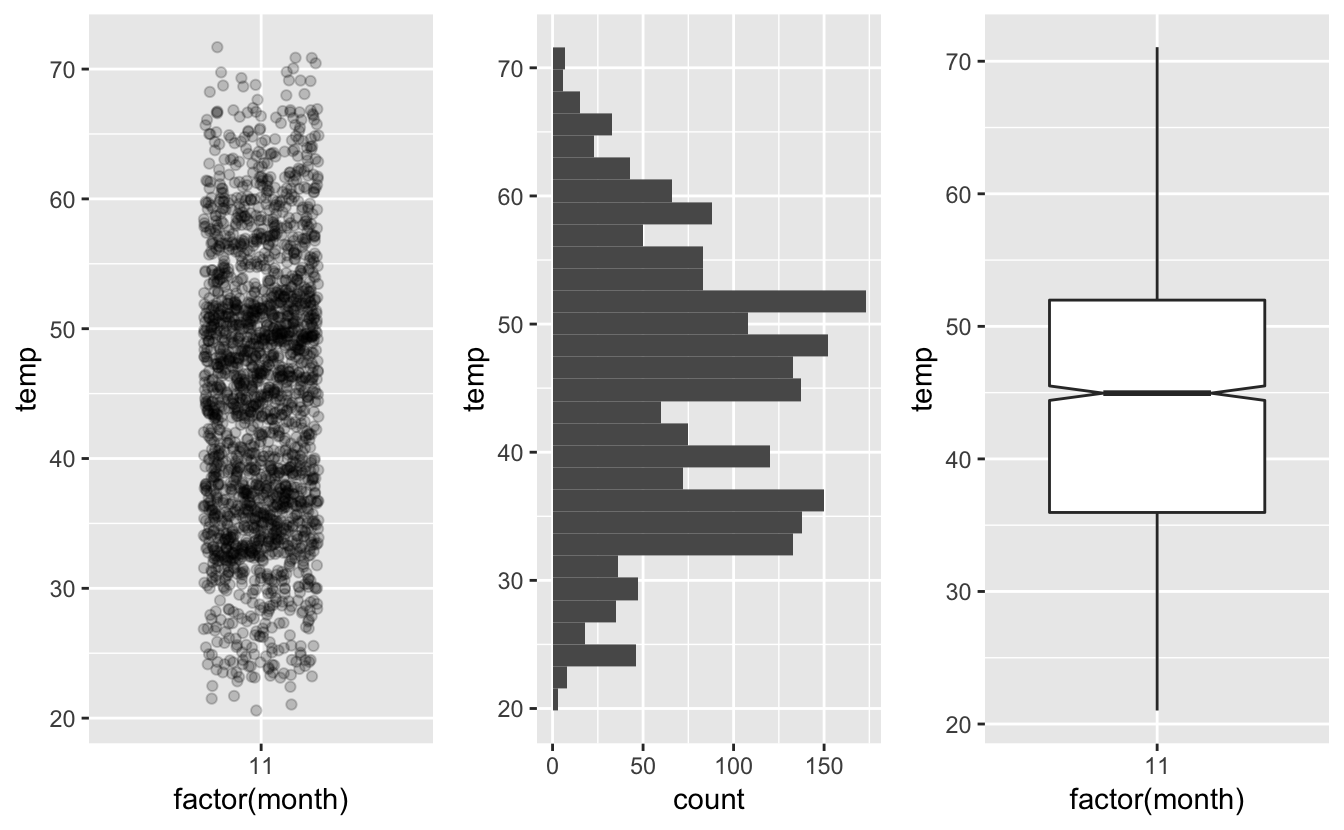
\includegraphics[width=0.9\linewidth]{figure/compboxplot-1} 

}

\caption{Distribution des températures de Novembre 2013.}\label{fig:compboxplot}
\end{figure}

Nous avons donc, à gauche les données brutes, sous la forme d'un nuage de points créé avec \texttt{geom\_jitter()}, au centre, un histogramme pour les températures de novembre, créé avec \texttt{geom\_histogram()} (j'ai permuté les axes pour que \texttt{y} porte la température pour les 3 graphiques) et à droite, un boxplot pour ces mêmes données, créé avec \texttt{geom\_boxplot()}. On voit bien que ces 3 représentations graphiques sont similaires. Toutes rendent compte du fait que les températures de Novembre sont majoritairement comprises entre 35 et 52 degrés Farenheit. Au-delà de cette fourchette (au-dessus comme en dessous) les observations sont plus rares.

Le nuage de points affiche toutes les données. C'est donc lui le plus complet mais pas forcément le plus lisible. Les points sont en effet très nombreux et la lecture du graphique peut s'en trouver compliquée. L'histogramme simplifie les données en les regroupant dans des classes. C'est une sorte de résumé des données. On constate cependant toujours la présence de 2 pics qui correspondent aux zones plus denses du nuage de points. Le boxplot enfin synthétise encore plus ces données. Elles sont résumées par 7 valeurs seulement : le minimum, le maximum, les 3 quartiles, et les bornes de l'intervalle de confiance à 95\% de la médiane. C'est une représentation très synthétique qui nous permet de comparer beaucoup de catégories côte à côte (voir la figure \ref{fig:notchedboxplot} un peu plus haut), mais qui est forcément moins précise qu'un histogramme. Vous noterez toutefois que la boîte du boxplot recouvre en grande partie la zone des 2 pics de l'histogramme. En outre, sur la figure \ref{fig:notchedboxplot}, la tendance générale est très visible : il fait plus chaud en été qu'en hiver (étonnant non ?).

\hypertarget{pour-conclure}{%
\subsubsection{Pour conclure}\label{pour-conclure}}

Les boîtes à moustaches permettent donc de comparer et contraster la distribution d'\textbf{une variable quantitative} pour plusieurs niveaux d'\textbf{une variable catégorielle}. On peut voir où la médiane tombe dans les différents groupes en observant la position de la ligne centrale dans la boîte. Pour avoir une idée de la dispersion de la variable au sein de chaque groupe, regardez à la fois la hauteur de la boîte et la longueur des moustaches. Quand les moustaches s'étendent loin de la boîte mais que la boîte est petite, cela signifie que la variabilité des valeurs proches du centre de la distribution est beaucoup plus faible que la variabilité des valeurs extrêmes. Enfin, les valeurs extrêmes ou aberrantes sont encore plus faciles à détecter avec une boîte à moustaches qu'avec un histogramme.

\begin{center}\rule{0.5\linewidth}{0.5pt}\end{center}

\hypertarget{les-diagrammes-buxe2tons}{%
\subsection{Les diagrammes bâtons}\label{les-diagrammes-buxe2tons}}

Comme nous venons de le voir, les histogrammes et les boîtes à moustaches permettent de visualiser la distribution d'une \textbf{variable numérique continue}. Nous aurons aussi souvent besoin de visualiser la distribution d'une \textbf{variable catégorielle}. C'est une tâche plus simple qui consiste à compter combien d'éléments tombent dans chacune des catégories de la variable catégorielle. Le meilleur moyen de visualiser de telles données de comptage (\emph{aka} fréquences) est de réaliser un diagramme bâtons, autrement appelé \textbf{barplot} ou \textbf{barchart}.

Une difficulté, toutefois, concerne la façon dont les données sont présentées : est-ce que la variable d'intérêt est ``pré-comptée'' ou non ? Par exemple, le code ci-dessous crée 2 \texttt{data.frame} qui représentent la même collection de fruits : 3 pommes et 2 oranges :

\begin{Shaded}
\begin{Highlighting}[]
\NormalTok{fruits <-}\StringTok{ }\KeywordTok{data_frame}\NormalTok{(}\DataTypeTok{fruit =} \KeywordTok{c}\NormalTok{(}\StringTok{"pomme"}\NormalTok{, }\StringTok{"pomme"}\NormalTok{, }\StringTok{"pomme"}\NormalTok{, }\StringTok{"orange"}\NormalTok{, }\StringTok{"orange"}\NormalTok{))}
\NormalTok{fruits}
\end{Highlighting}
\end{Shaded}

\begin{verbatim}
# A tibble: 5 x 1
  fruit 
  <chr> 
1 pomme 
2 pomme 
3 pomme 
4 orange
5 orange
\end{verbatim}

\begin{Shaded}
\begin{Highlighting}[]
\NormalTok{fruits_counted <-}\StringTok{ }\KeywordTok{data_frame}\NormalTok{(}\DataTypeTok{fruit =} \KeywordTok{c}\NormalTok{(}\StringTok{"pomme"}\NormalTok{, }\StringTok{"orange"}\NormalTok{), }\DataTypeTok{nombre =} \KeywordTok{c}\NormalTok{(}\DecValTok{3}\NormalTok{, }
    \DecValTok{2}\NormalTok{))}
\NormalTok{fruits_counted}
\end{Highlighting}
\end{Shaded}

\begin{verbatim}
# A tibble: 2 x 2
  fruit  nombre
  <chr>   <dbl>
1 pomme       3
2 orange      2
\end{verbatim}

\hypertarget{repruxe9sentation-graphique-avec-geom_bar-et-geom_col}{%
\subsubsection{\texorpdfstring{Représentation graphique avec \texttt{geom\_bar} et \texttt{geom\_col}}{Représentation graphique avec geom\_bar et geom\_col}}\label{repruxe9sentation-graphique-avec-geom_bar-et-geom_col}}

Pour visualiser les données non pré-comptées, on utilise \texttt{geom\_bar()} :

\begin{Shaded}
\begin{Highlighting}[]
\KeywordTok{ggplot}\NormalTok{(}\DataTypeTok{data =}\NormalTok{ fruits, }\DataTypeTok{mapping =} \KeywordTok{aes}\NormalTok{(}\DataTypeTok{x =}\NormalTok{ fruit)) }\OperatorTok{+}
\StringTok{  }\KeywordTok{geom_bar}\NormalTok{()}
\end{Highlighting}
\end{Shaded}

\begin{figure}[htpb]

{\centering 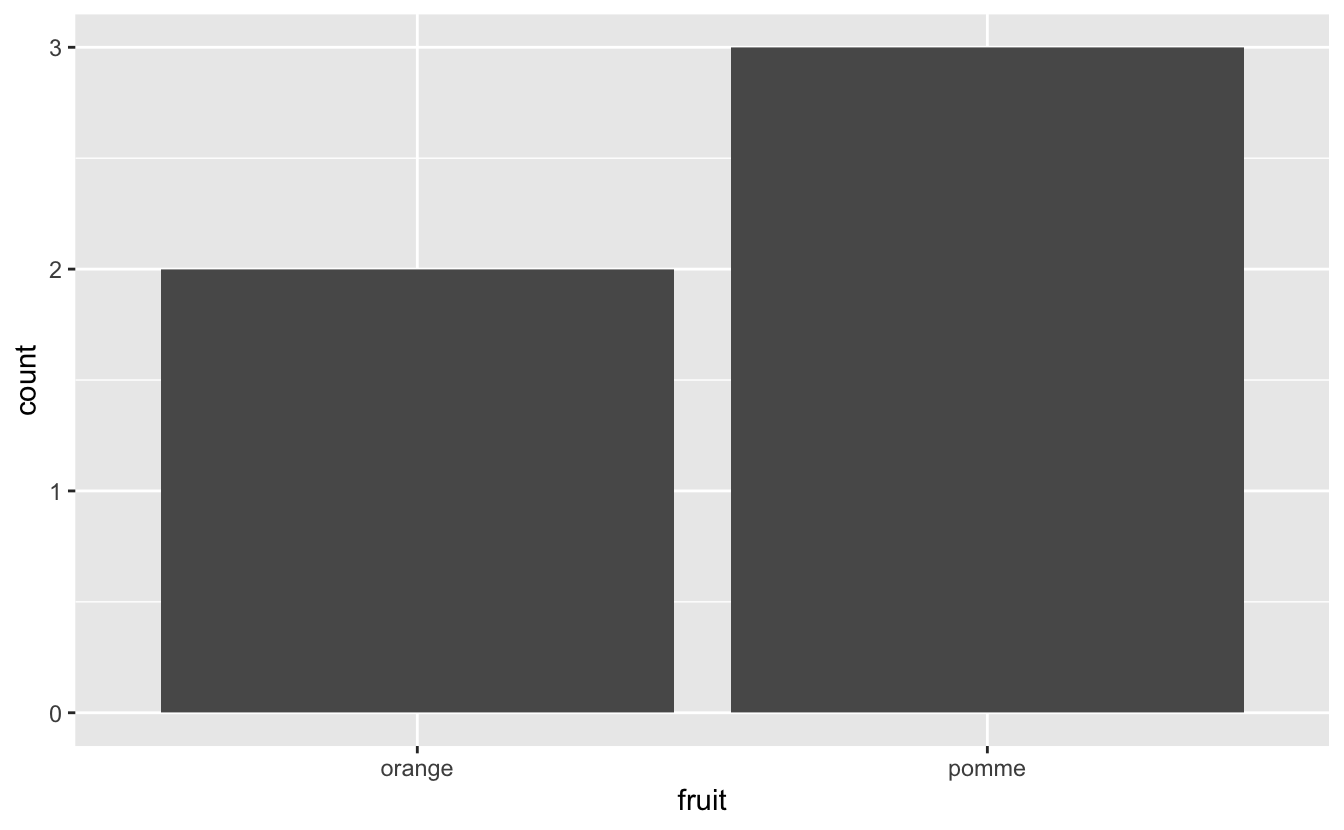
\includegraphics[width=0.9\linewidth]{figure/barplot-1} 

}

\caption{Barplot pour des données non pré-comptées.}\label{fig:barplot}
\end{figure}

Pour visualiser les données déjà pré-comptées, on utilise \texttt{geom\_col()} :

\begin{Shaded}
\begin{Highlighting}[]
\KeywordTok{ggplot}\NormalTok{(}\DataTypeTok{data =}\NormalTok{ fruits_counted, }\DataTypeTok{mapping =} \KeywordTok{aes}\NormalTok{(}\DataTypeTok{x =}\NormalTok{ fruit, }\DataTypeTok{y =}\NormalTok{ nombre)) }\OperatorTok{+}
\StringTok{  }\KeywordTok{geom_col}\NormalTok{()}
\end{Highlighting}
\end{Shaded}

\begin{figure}[htpb]

{\centering 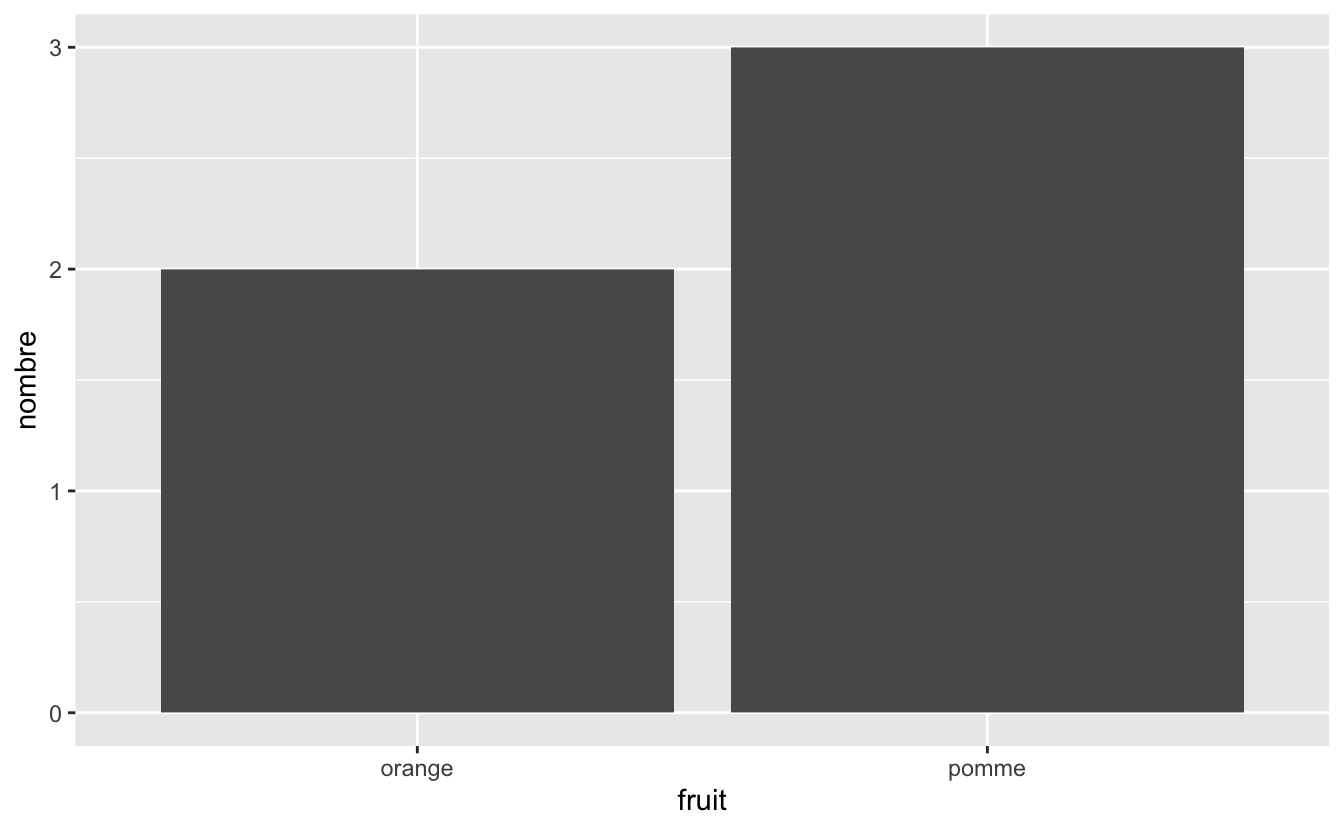
\includegraphics[width=0.9\linewidth]{figure/barplotcol-1} 

}

\caption{Barplot pour des données pré-comptées.}\label{fig:barplotcol}
\end{figure}

Notez que les figures \ref{fig:barplot} et \ref{fig:barplotcol} sont absolument identiques (à l'exception du titre de l'axe des ordonnées), mais qu'elles ont été créées à partir de 2 tableaux de données différents. En particulier, notez que :

\begin{itemize}
\tightlist
\item
  Le code qui génère la figure \ref{fig:barplot} utilise le jeu de données \texttt{fruits}, et n'associe pas de variable à l'axe des ordonnées : dans la fonction \texttt{aes()}, seule la variable associée à \texttt{x} est précisée. C'est la fonction \texttt{geom\_bar()} qui calcule automatiquement les abondances (ou fréquences) pour chaque catégorie de la variable \texttt{fruit}. La variable \texttt{count} est ainsi générée automatiquement et associée à \texttt{y}.
\item
  Le code qui génère la figure \ref{fig:barplotcol} utilise le jeu de données \texttt{fruits\_counted}. Ici, la variable \texttt{nombre} est associée à l'axe des \texttt{y} grâce à la fonction \texttt{aes()}. La fonction \texttt{geom\_col()} a besoin de 2 variables (une variable catégorielle pour l'axe des \texttt{x} et une numérique pour l'axe des \texttt{y}) pour fonctionner.
\end{itemize}

Autrement dit, lorsque vous souhaiterez créer un diagramme bâtons, il faudra donc au préalable vérifier de quel type de données vous disposez pour choisir l'objet géométrique approprié :

\begin{itemize}
\tightlist
\item
  Si votre variable catégorielle n'est pas pré-comptée dans votre tableau de données, il faut utiliser \texttt{geom\_bar()}
\item
  Si votre variable catégorielle est pré-comptée dans votre tableau de données, il faut utiliser \texttt{geom\_col()} et associer explicitement les comptages à l'aesthétique \texttt{y} du graphique.
\end{itemize}

\hypertarget{un-exemple-concret}{%
\subsubsection{Un exemple concret}\label{un-exemple-concret}}

Revenons à \texttt{nycflights13}. Imaginons que nous souhaitions connaître le nombre de vols affrétés par chaque compagnie aérienne au départ de New York en 2013. Dans le jeu de données \texttt{flights}, la variable \texttt{carrier} nous indique à quelle compagnie aérienne appartiennent chacun des 336776 vols ayant quitté New York en 2013. Une façon simple de représenter ces données est donc la suivante :

\begin{Shaded}
\begin{Highlighting}[]
\KeywordTok{ggplot}\NormalTok{(}\DataTypeTok{data =}\NormalTok{ flights, }\DataTypeTok{mapping =} \KeywordTok{aes}\NormalTok{(}\DataTypeTok{x =}\NormalTok{ carrier)) }\OperatorTok{+}
\StringTok{  }\KeywordTok{geom_bar}\NormalTok{()}
\end{Highlighting}
\end{Shaded}

\begin{figure}[htpb]

{\centering \includegraphics[width=0.9\linewidth]{figure/bpcarrier-1} 

}

\caption{Nombre de vols par compagnie aérienne au départ de New York en 2013.}\label{fig:bpcarrier}
\end{figure}

Ici, \texttt{geom\_bar()} a compté le nombre d'occurences de chaque compagnie aérienne dans le tableau \texttt{flights} et a automatiquement associé ce nombre à l'axe des ordonnées.

Il est généralement plus utile de trier les catégories par ordre décroissant. Nous pouvons faire cela facilement grâce à la fonction \texttt{fct\_infreq()} du package \texttt{forcats}. Si vous avez installé le \texttt{tidyverse}, le package \texttt{forcast} doit être disponible sur votre ordinateur. N'oubliez pas de le charger si besoin :

\begin{Shaded}
\begin{Highlighting}[]
\KeywordTok{library}\NormalTok{(forcats)}
\KeywordTok{ggplot}\NormalTok{(}\DataTypeTok{data =}\NormalTok{ flights, }\DataTypeTok{mapping =} \KeywordTok{aes}\NormalTok{(}\DataTypeTok{x =} \KeywordTok{fct_infreq}\NormalTok{(carrier))) }\OperatorTok{+}
\StringTok{  }\KeywordTok{geom_bar}\NormalTok{()}
\end{Highlighting}
\end{Shaded}

\begin{figure}[htpb]

{\centering \includegraphics[width=0.9\linewidth]{figure/bpcarriersorted-1} 

}

\caption{Nombre de vols par compagnie aérienne au départ de New York en 2013.}\label{fig:bpcarriersorted}
\end{figure}

Ordonner les catégories par ordre décroissant est souvent indispensable afin de faciliter la lecture du graphique et les comparaisons entre catégories.

Si nous souhaitons connaître le nombre de vols précis de chaque compagnie aérienne, il nous faut faire appel à plusieurs fonctions du package \texttt{dplyr} que nous détaillerons dans le chapitre \ref{wrangling}. Ci-dessous, nous créons un nouveau tableau \texttt{carrier\_table} contenant le nombre de vols de chaque compagnie aérienne et les compagnies sont ordonnées par nombres de vols décroissants :

\begin{Shaded}
\begin{Highlighting}[]
\NormalTok{carrier_table <-}\StringTok{ }\NormalTok{flights }\OperatorTok\StringTok{   }\CommentTok{# On prend flights, puis...}
\StringTok{  }\KeywordTok{group_by}\NormalTok{(carrier) }\OperatorTok\StringTok{        }\CommentTok{# On groupe les données par compagnie, puis...}
\StringTok{  }\KeywordTok{summarize}\NormalTok{(}\DataTypeTok{nombre =} \KeywordTok{n}\NormalTok{()) }\OperatorTok\StringTok{  }\CommentTok{# On calcule le nb de vols par Cie, puis ...}
\StringTok{  }\KeywordTok{arrange}\NormalTok{(}\KeywordTok{desc}\NormalTok{(nombre))        }\CommentTok{# On trie par nb de vols décroissants ...}
\end{Highlighting}
\end{Shaded}

\begin{verbatim}
`summarise()` ungrouping output (override with `.groups` argument)
\end{verbatim}

\begin{Shaded}
\begin{Highlighting}[]
\NormalTok{carrier_table                  }\CommentTok{# Enfin, on affiche la nouvelle table}
\end{Highlighting}
\end{Shaded}

\begin{verbatim}
# A tibble: 16 x 2
   carrier nombre
   <chr>    <int>
 1 UA       58665
 2 B6       54635
 3 EV       54173
 4 DL       48110
 5 AA       32729
 6 MQ       26397
 7 US       20536
 8 9E       18460
 9 WN       12275
10 VX        5162
11 FL        3260
12 AS         714
13 F9         685
14 YV         601
15 HA         342
16 OO          32
\end{verbatim}

Ici, la table a été triée par nombres de vols décroissants. Mais attention, \textbf{les niveaux} du facteur \texttt{carrier} n'ont pas été modifiés :

\begin{Shaded}
\begin{Highlighting}[]
\KeywordTok{factor}\NormalTok{(carrier_table}\OperatorTok{$}\NormalTok{carrier)}
\end{Highlighting}
\end{Shaded}

\begin{verbatim}
 [1] UA B6 EV DL AA MQ US 9E WN VX FL AS F9 YV HA OO
Levels: 9E AA AS B6 DL EV F9 FL HA MQ OO UA US VX WN YV
\end{verbatim}

Le premier niveau est toujours \texttt{9E}, puis \texttt{AA}, puis \texttt{AS}, et non l'ordre du tableau nouvellement créé (\texttt{UA}, puis \texttt{B6}, puis \texttt{EV}\ldots) car les niveaux sont toujours triés par ordre alphabétique. La conséquence est que faire un barplot avec ces données et la fonction \texttt{geom\_col()} ne permet pas d'ordonner les catégories correctement :

\begin{Shaded}
\begin{Highlighting}[]
\KeywordTok{ggplot}\NormalTok{(carrier_table, }\KeywordTok{aes}\NormalTok{(}\DataTypeTok{x =}\NormalTok{ carrier, }\DataTypeTok{y =}\NormalTok{ nombre)) }\OperatorTok{+}
\StringTok{  }\KeywordTok{geom_col}\NormalTok{()}
\end{Highlighting}
\end{Shaded}

\begin{figure}[htpb]

{\centering \includegraphics[width=0.9\linewidth]{figure/bpcarriercol-1} 

}

\caption{Nombre de vols par compagnie aérienne au départ de New York en 2013.}\label{fig:bpcarriercol}
\end{figure}

Pour parvenir à nos fins, il faut cette fois avoir recours à la fonction \texttt{fct\_reorder()} pour ordonner correctement les catégories. Cette fonction prends 3 arguments :

\begin{enumerate}
\def\labelenumi{\arabic{enumi}.}
\tightlist
\item
  La variable catégorielle dont on souhaite réordonner les niveaux (ici, la variable \texttt{carrier} du tableau \texttt{carrier\_table}).
\item
  Une variable numérique qui permet d'ordonner les catégories (ici, la variable \texttt{nombre} du même tableau).
\item
  L'argument optionnel \texttt{.desc} qui permet de préciser si le tri doit être fait en ordre croissant (c'est le cas par défaut) ou décroissant.
\end{enumerate}

\begin{Shaded}
\begin{Highlighting}[]
\KeywordTok{ggplot}\NormalTok{(carrier_table, }\KeywordTok{aes}\NormalTok{(}\DataTypeTok{x =} \KeywordTok{fct_reorder}\NormalTok{(carrier, nombre, }\DataTypeTok{.desc =} \OtherTok{TRUE}\NormalTok{), }
                          \DataTypeTok{y =}\NormalTok{ nombre)) }\OperatorTok{+}
\StringTok{  }\KeywordTok{geom_col}\NormalTok{()}
\end{Highlighting}
\end{Shaded}

\begin{figure}[htpb]

{\centering \includegraphics[width=0.9\linewidth]{figure/bpcarriersortedcol-1} 

}

\caption{Nombre de vols par compagnie aérienne au départ de New York en 2013.}\label{fig:bpcarriersortedcol}
\end{figure}

Vous voyez donc que selon le type de données dont vous disposez (soit un tableau comme \texttt{flights}, avec toutes les observations, soit un tableau beaucoup plus compact comme \texttt{carrier\_table}), la démarche permettant de produire un diagramme bâtons, dans lequel les catégories seront triées, sera différente.

\hypertarget{exercices-5}{%
\subsubsection{Exercices}\label{exercices-5}}

\begin{enumerate}
\def\labelenumi{\arabic{enumi}.}
\tightlist
\item
  Quelle est la différence entre un histogramme et un diagramme bâtons ?
\item
  Pourquoi les histogrammes sont-ils inadaptés pour visualiser des données catégorielles ?
\item
  Quel est le nom de la compagnie pour laquelle le plus grand nombre de vols ont quitté New York en 2013 (je veux connaître son nom, pas juste son code) ? Où se trouve cette information ?
\item
  Quel est le nom de la compagnie pour laquelle le plus petit nombre de vols ont quitté New York en 2013 (je veux connaître son nom, pas juste son code) ? Où se trouve cette information ?
\end{enumerate}

\hypertarget{uxe9viter-uxe0-tout-prix-les-diagrammes-circulaires}{%
\subsubsection{Éviter à tout prix les diagrammes circulaires}\label{uxe9viter-uxe0-tout-prix-les-diagrammes-circulaires}}

À mon grand désarroi, l'un des graphiques les plus utilisé pour représenter la distribution d'une variable catégorielle est le diagramme circulaire (ou diagramme camembert, piechart en anglais). C'est presque toujours la plus mauvaise visualisation possible. Je vous demande de l'éviter à tout prix. Notre cerveau n'est en effet pas correctement équipé pour comparer des angles. Ainsi, par exemple, nous avons naturellement tendance à surestimer les angles supérieurs à 90º, et à sous-estimer les angles inférieurs à 90º. En d'autres termes, il est difficile pour les humains de comparer des grandeurs sur des diagrammes circulaires.

À titre d'exemple, examinez ce diagramme, qui reprend les mêmes chiffres que précédemment, et tentez de répondre aux questions suivantes :

\begin{figure}[htpb]

{\centering \includegraphics[width=0.9\linewidth]{figure/piechart-1} 

}

\caption{Nombre de vols par compagnie aérienne au départ de New York en 2013.}\label{fig:piechart}
\end{figure}

\begin{itemize}
\tightlist
\item
  Comparez les compagnies ExpressJet Airlines (\texttt{EV}) et US Airways (\texttt{US}). De combien de fois la part de \texttt{EV} est-elle supérieure à celle d'\texttt{US} ? (2 fois, 3 fois, 1.2 fois ?\ldots)
\item
  Quelle est la troisième compagnie aérienne la plus importante en terme de nombre de vols au départ de New York en 2013 ?
\item
  Combien de compagnies aériennes ont moins de vols que United Airlines (\texttt{UA}) ?
\end{itemize}

Il est difficile (voir impossible) de répondre précisément à ces questions avec le diagramme circulaire de la figure \ref{fig:piechart}, alors qu'il est très simple d'obtenir des réponses précises avec un diagramme bâtons tel que présenté à la figure \ref{fig:bpcarriersortedcol} (vérifiez-le !).

\hypertarget{comparer-2-variables-catuxe9gorielles-avec-un-diagramme-buxe2ton}{%
\subsubsection{Comparer 2 variables catégorielles avec un diagramme bâton}\label{comparer-2-variables-catuxe9gorielles-avec-un-diagramme-buxe2ton}}

Il y a généralement 3 façons de procéder pour comparer la distribution de 2 variables catégorielles avec un diagramme bâtons :

\begin{enumerate}
\def\labelenumi{\arabic{enumi}.}
\tightlist
\item
  Faire un graphique empilé.
\item
  Faire un graphique juxtaposé.
\item
  Utiliser les \texttt{facet}s.
\end{enumerate}

Supposons par exemple que nous devions visualiser le nombre de vols de chaque compagnie aérienne, au départ de chacun des 3 aéroports de New York : John F. Kennedy (\texttt{JFK}), Newark (\texttt{EWR}) et La Guardia (\texttt{LGA}). Voyons comment procéder avec chacune des 3 méthodes énoncées ci-dessus.

\hypertarget{graphique-empiluxe9}{%
\paragraph{Graphique empilé}\label{graphique-empiluxe9}}

La méthode la plus simple est celle du graphique empilé :

\begin{Shaded}
\begin{Highlighting}[]
\KeywordTok{ggplot}\NormalTok{(flights, }\KeywordTok{aes}\NormalTok{(}\DataTypeTok{x =} \KeywordTok{fct_infreq}\NormalTok{(carrier), }\DataTypeTok{fill =}\NormalTok{ origin)) }\OperatorTok{+}
\StringTok{  }\KeywordTok{geom_bar}\NormalTok{()}
\end{Highlighting}
\end{Shaded}

\begin{figure}[htpb]

{\centering \includegraphics[width=0.9\linewidth]{figure/stacked-1} 

}

\caption{Nombre de vols par compagnie aérienne au départ des 3 aéroports de New York en 2013.}\label{fig:stacked}
\end{figure}

Notez qu'il s'agit du même code que celui utilisé pour la figure \ref{fig:bpcarriersorted}, à une différence près : l'ajout de \texttt{fill\ =\ origin} dans la fonction \texttt{aes()}, qui permet d'associer l'aéroport d'origine à la couleur de remplissage des barres. \texttt{fill} est associé à une variable (ici, elle est catégorielle), il est donc indispensable de faire figurer cet argument à l'intérieur de la fonction \texttt{aes()}. Quand on associe une variable à une caractéristique esthétique du graphique, on fait toujours figurer le code à l'intérieur de la fonction \texttt{aes()} (comme quand on associe une variable aux axes du graphique par exemple).

À mon sens, le graphique gagne en lisibilité si on ajoute une couleur pour le contour des barres :

\begin{Shaded}
\begin{Highlighting}[]
\KeywordTok{ggplot}\NormalTok{(flights, }\KeywordTok{aes}\NormalTok{(}\DataTypeTok{x =} \KeywordTok{fct_infreq}\NormalTok{(carrier), }\DataTypeTok{fill =}\NormalTok{ origin)) }\OperatorTok{+}
\StringTok{  }\KeywordTok{geom_bar}\NormalTok{(}\DataTypeTok{color =} \StringTok{"black"}\NormalTok{)}
\end{Highlighting}
\end{Shaded}

\begin{figure}[htpb]

{\centering \includegraphics[width=0.9\linewidth]{figure/stacked2-1} 

}

\caption{Nombre de vols par compagnie aérienne au départ des 3 aéroports de New York en 2013.}\label{fig:stacked2}
\end{figure}

Notez que contrairement à \texttt{fill}, cette couleur de countour est un paramètre fixe : elle n'est pas associée à une variable et doit donc être placée en dehors de la fonction \texttt{aes()}.

Bien que ces graphiques empilés soient très simples à réaliser, ils sont parfois difficiles à lire. En particulier, il n'est pas toujours aisé de comparer les hauteurs des différentes couleurs (qui correspondent ici aux nombres de vols issus de chaque aéroport) entre barres différentes (qui correspondent ici aux compagnies aériennes).

\hypertarget{graphique-juxtaposuxe9}{%
\paragraph{Graphique juxtaposé}\label{graphique-juxtaposuxe9}}

Une variation sur le même thème consiste, non plus à empiler les barres de couleur les unes sur les autres, mais à les juxtaposer :

\begin{Shaded}
\begin{Highlighting}[]
\KeywordTok{ggplot}\NormalTok{(flights, }\KeywordTok{aes}\NormalTok{(}\DataTypeTok{x =} \KeywordTok{fct_infreq}\NormalTok{(carrier), }\DataTypeTok{fill =}\NormalTok{ origin)) }\OperatorTok{+}
\StringTok{  }\KeywordTok{geom_bar}\NormalTok{(}\DataTypeTok{color =} \StringTok{"black"}\NormalTok{, }\DataTypeTok{position =} \StringTok{"dodge"}\NormalTok{)}
\end{Highlighting}
\end{Shaded}

\begin{figure}[htpb]

{\centering \includegraphics[width=0.9\linewidth]{figure/dodge-1} 

}

\caption{Nombre de vols par compagnie aérienne au départ des 3 aéroports de New York en 2013.}\label{fig:dodge}
\end{figure}

Passer d'un graphique empilé à un graphique juxtaposé est donc très simple : il suffit d'ajouter l'argument \texttt{position\ =\ "dodge"} à la fonction \texttt{geom\_bar()}.

Là encore, la lecture de ces graphiques est souvent difficile car la comparaison des catégories qui figurent sur l'axe des \texttt{x} n'est pas immédiate. Elle est en outre rendue plus difficile par le fait que toutes les barres n'ont pas la même largeur. Par exemple, sur la figure \ref{fig:dodge}, les 8 premières compagnies aériennes déservent les 3 aéroports de New York, mais les 2 suivantes (\texttt{WN} et \texttt{VX}) n'en déservent que 2, et les autres compagnies, qu'un seul. Puisque sur un barplot, seule la hauteur des barres compte, il faut prendre garde à ne pas se laisser influencer par la largeur des barres qui pourraient fausser notre perception.

\hypertarget{utilisation-des-facets}{%
\paragraph{\texorpdfstring{Utilisation des \texttt{facet}s}{Utilisation des facets}}\label{utilisation-des-facets}}

La meilleure alternative est probablement l'utilisation de \texttt{facet}s que nous avons déjà décrite à la section \ref{facets} :

\begin{Shaded}
\begin{Highlighting}[]
\KeywordTok{ggplot}\NormalTok{(flights, }\KeywordTok{aes}\NormalTok{(}\DataTypeTok{x =} \KeywordTok{fct_infreq}\NormalTok{(carrier), }\DataTypeTok{fill =}\NormalTok{ origin)) }\OperatorTok{+}
\StringTok{  }\KeywordTok{geom_bar}\NormalTok{(}\DataTypeTok{color =} \StringTok{"black"}\NormalTok{) }\OperatorTok{+}
\StringTok{  }\KeywordTok{facet_wrap}\NormalTok{(}\OperatorTok{~}\NormalTok{origin, }\DataTypeTok{ncol =} \DecValTok{1}\NormalTok{)}
\end{Highlighting}
\end{Shaded}

\begin{figure}[htpb]

{\centering \includegraphics[width=0.9\linewidth]{figure/barfacet-1} 

}

\caption{Nombre de vols par compagnie aérienne au départ des 3 aéroports de New York en 2013.}\label{fig:barfacet}
\end{figure}

Ici, chaque graphique permet de comparer les compagnies aériennes au sein de l'un des aéroports de New York, et puisque l'ordre des compagnies aériennes est le même sur l'axe des \texttt{x} des 3 graphiques, une lecture verticale permet de comparer aisément le nombre de vols qu'une compagnie donnée a affrété dans chacun des 3 aéroports de New York.

\begin{center}\rule{0.5\linewidth}{0.5pt}\end{center}

\hypertarget{de-lexploration-uxe0-lexposition}{%
\subsection{De l'exploration à l'exposition}\label{de-lexploration-uxe0-lexposition}}

Vous savez maintenant comment produire une grande variété de graphiques, permettant d'explorer vos données, de visualiser le comportement d'une ou plusieurs variables, et de mettre en évidence des tendances, des relations entre variables numériques et/ou catégorielles. Outre les objets géométriques décrits jusqu'ici, \texttt{ggplot2} contient de nombreuses possibilités supplémentaires pour créer des graphiques parlants et originaux. Je ne peux donc que vous encourager à explorer par vous même les autres possibilités de ce package.
Lorsque vous produisez un graphique parlant et permettant de véhiculer un message clair, vous devez ensuite rendre vos graphiques plus présentables afin de les intégrer dans un rapport ou une présentation. Cette section vous permettra de vous familiariser avec quelques fonctions permettant d'annoter correctement vos graphiques et d'en modifier les légendes si nécessaire.

\hypertarget{les-labels}{%
\subsubsection{Les labels}\label{les-labels}}

Le point de départ le plus évident est d'ajouter des labels de qualité. La fonction \texttt{labs()} du package \texttt{ggplot2} permet d'ajouter plusieurs types de labels sur vos graphiques :

\begin{itemize}
\tightlist
\item
  Un titre : il doit résumer les résultats les plus importants.
\item
  Un sous-titre : il permet de donner quelques détails supplémentaires.
\item
  Une légende : souvent utilisée pour présenter la source des données du graphique.
\item
  Un titre pour chaque axe : permet de préciser les variables portées par les axes et leurs unités.
\item
  Un titre pour les légendes de couleurs, de forme, de taille, etc.
\end{itemize}

Reprenons par exemple le graphique de la figure \ref{fig:varcolor} :

\begin{Shaded}
\begin{Highlighting}[]
\KeywordTok{ggplot}\NormalTok{(alaska_flights, }
       \KeywordTok{aes}\NormalTok{(}\DataTypeTok{x =}\NormalTok{ dep_delay, }\DataTypeTok{y =}\NormalTok{ arr_delay, }\DataTypeTok{color =} \KeywordTok{factor}\NormalTok{(month))) }\OperatorTok{+}
\StringTok{  }\KeywordTok{geom_point}\NormalTok{()}
\end{Highlighting}
\end{Shaded}

\begin{figure}[htpb]

{\centering \includegraphics[width=0.9\linewidth]{figure/varcolorlabel-1} 

}

\caption{Association de `color` à une variable catégorielle.}\label{fig:varcolorlabel}
\end{figure}

Nous pouvons ajouter sur ce graphique les éléments précisés plus haut en ajoutant la fonction \texttt{labs()} sur une nouvelle couche du graphique :

\begin{Shaded}
\begin{Highlighting}[]
\KeywordTok{ggplot}\NormalTok{(alaska_flights, }
       \KeywordTok{aes}\NormalTok{(}\DataTypeTok{x =}\NormalTok{ dep_delay, }\DataTypeTok{y =}\NormalTok{ arr_delay, }\DataTypeTok{color =} \KeywordTok{factor}\NormalTok{(month))) }\OperatorTok{+}
\StringTok{  }\KeywordTok{geom_point}\NormalTok{() }\OperatorTok{+}
\StringTok{  }\KeywordTok{labs}\NormalTok{(}\DataTypeTok{title =} \StringTok{"Relation linéaire positive entre retard des vols au départ et à l'arrivée"}\NormalTok{,}
       \DataTypeTok{subtitle =} \StringTok{"Certains retards dépassent 3 heures"}\NormalTok{,}
       \DataTypeTok{caption =} \StringTok{"Source : nycflights13"}\NormalTok{,}
       \DataTypeTok{x =} \StringTok{"Retard au départ de New York (minutes)"}\NormalTok{,}
       \DataTypeTok{y =} \StringTok{"Retard à l'arrivée à destination (minutes)"}\NormalTok{,}
       \DataTypeTok{color =} \StringTok{"Mois"}\NormalTok{)}
\end{Highlighting}
\end{Shaded}

\begin{figure}[htpb]

{\centering \includegraphics[width=0.9\linewidth]{figure/varcolorlabel2-1} 

}

\caption{Exemple d'utilisation de `labs()`.}\label{fig:varcolorlabel2}
\end{figure}

À partir de maintenant, vous devriez systématiquement légender les axes de vos graphiques en n'oubliant pas de préciser les unités, pour tous les graphiques que vous intégrez dans vos rapports, compte-rendus, mémoires, etc.

\hypertarget{les-uxe9chelles}{%
\subsubsection{Les échelles}\label{les-uxe9chelles}}

Tous les détails des graphiques que vous produisez peuvent être édités. C'est notamment le cas des échelles. Qu'il s'agisse de modifier l'étendue des axes, la densité du quadrillage, la position des tirets sur les axes, le nom des catégories figurant sur les axes ou dans les légendes ou encore les couleurs utilisées pour différentes catégories d'objets géométriques, tout est possible dans \texttt{ggplot2}.

Nous n'avons pas le temps ici d'aborder toutes ces questions en détail. Je vous encourage donc à consulter l'ouvrage en ligne intitulé \href{http://r4ds.had.co.nz/}{R for data science}, et en particulier \href{http://r4ds.had.co.nz/graphics-for-communication.html\#scales}{son chapitre dédié aux échelles}, si vous avez besoin d'apporter des modifications à vos graphiques et que vous ne trouvez pas comment faire dans cet ouvrage.

Je vais ici uniquement détailler la façon de procéder pour modifier les couleurs choisies par défaut par \texttt{ggplot2}. Reprenons par exemple la figure \ref{fig:barfacet}, en ajoutant au passage des titres corrects pour nos axes

\begin{Shaded}
\begin{Highlighting}[]
\KeywordTok{ggplot}\NormalTok{(flights, }\KeywordTok{aes}\NormalTok{(}\DataTypeTok{x =} \KeywordTok{fct_infreq}\NormalTok{(carrier), }\DataTypeTok{fill =}\NormalTok{ origin)) }\OperatorTok{+}
\StringTok{  }\KeywordTok{geom_bar}\NormalTok{(}\DataTypeTok{color =} \StringTok{"black"}\NormalTok{) }\OperatorTok{+}
\StringTok{  }\KeywordTok{facet_wrap}\NormalTok{(}\OperatorTok{~}\NormalTok{origin, }\DataTypeTok{ncol =} \DecValTok{1}\NormalTok{) }\OperatorTok{+}
\StringTok{  }\KeywordTok{labs}\NormalTok{(}\DataTypeTok{x =} \StringTok{"Compagnie aérienne"}\NormalTok{,}
       \DataTypeTok{y =} \StringTok{"Nombre de vols"}\NormalTok{,}
       \DataTypeTok{fill =} \StringTok{"Aéroports}\CharTok{\textbackslash{}n}\StringTok{de New York"}\NormalTok{)}
\end{Highlighting}
\end{Shaded}

\begin{figure}[htpb]

{\centering \includegraphics[width=0.9\linewidth]{figure/barfacetbis-1} 

}

\caption{Nombre de vols par compagnie aérienne au départ des 3 aéroports de New York en 2013.}\label{fig:barfacetbis}
\end{figure}

Notez que le caractère spécial ``\texttt{\textbackslash{}n}'' permet de forcer un retour à la ligne. Ici, les 3 couleurs de remplissage (\texttt{fill}) utilisées pour différencier les 3 aéroports de New York ont été choisies par défaut par \texttt{ggplot2}. Il est possible de modifier ces couleurs de plusieurs façons :

\begin{itemize}
\tightlist
\item
  En utilisant d'autres palettes de couleurs prédéfinies.
\item
  En utilisant des couleurs choisies manuellement.
\end{itemize}

Toutes les fonctions permettant d'altérer les légendes commencent par \texttt{scale\_}. Vient ensuite le nom de l'esthétique que l'on souhaite modifier (ici \texttt{fill\_}) et enfin, le nom d'une fonction à appliquer. Les possibilités sont nombreuses et vous pouvez en avoir un aperçu en tapant le début du nom de la fonction et en parcourant la liste proposée par RStudio sous le curseur.

Par exemple, pour utiliser des niveaux de gris plutôt que les couleurs, il suffit d'ajouter une couche à notre graphique :

\begin{Shaded}
\begin{Highlighting}[]
\KeywordTok{ggplot}\NormalTok{(flights, }\KeywordTok{aes}\NormalTok{(}\DataTypeTok{x =} \KeywordTok{fct_infreq}\NormalTok{(carrier), }\DataTypeTok{fill =}\NormalTok{ origin)) }\OperatorTok{+}
\StringTok{  }\KeywordTok{geom_bar}\NormalTok{(}\DataTypeTok{color =} \StringTok{"black"}\NormalTok{) }\OperatorTok{+}
\StringTok{  }\KeywordTok{facet_wrap}\NormalTok{(}\OperatorTok{~}\NormalTok{origin, }\DataTypeTok{ncol =} \DecValTok{1}\NormalTok{) }\OperatorTok{+}
\StringTok{  }\KeywordTok{labs}\NormalTok{(}\DataTypeTok{x =} \StringTok{"Compagnie aérienne"}\NormalTok{,}
       \DataTypeTok{y =} \StringTok{"Nombre de vols"}\NormalTok{,}
       \DataTypeTok{fill =} \StringTok{"Aéroports}\CharTok{\textbackslash{}n}\StringTok{de New York"}\NormalTok{) }\OperatorTok{+}
\StringTok{  }\KeywordTok{scale_fill_grey}\NormalTok{()}
\end{Highlighting}
\end{Shaded}

\begin{figure}[htpb]

{\centering \includegraphics[width=0.9\linewidth]{figure/barfacetgray-1} 

}

\caption{Nombre de vols par compagnie aérienne au départ des 3 aéroports de New York en 2013.}\label{fig:barfacetgray}
\end{figure}

Le package \texttt{RColorBrewer} propose une large gamme de palettes de couleurs (figure \ref{fig:RcolorbrewerPalettes}) :

\begin{figure}[htpb]

{\centering \includegraphics[width=0.5\linewidth]{images/brewer} 

}

\caption{Toutes les palettes de couleur du package `RColorBrewer`.}\label{fig:RcolorbrewerPalettes}
\end{figure}

\texttt{ggplot2} permet d'appliquer ces palettes très simplement :

\begin{Shaded}
\begin{Highlighting}[]
\KeywordTok{ggplot}\NormalTok{(flights, }\KeywordTok{aes}\NormalTok{(}\DataTypeTok{x =} \KeywordTok{fct_infreq}\NormalTok{(carrier), }\DataTypeTok{fill =}\NormalTok{ origin)) }\OperatorTok{+}
\StringTok{  }\KeywordTok{geom_bar}\NormalTok{(}\DataTypeTok{color =} \StringTok{"black"}\NormalTok{) }\OperatorTok{+}
\StringTok{  }\KeywordTok{facet_wrap}\NormalTok{(}\OperatorTok{~}\NormalTok{origin, }\DataTypeTok{ncol =} \DecValTok{1}\NormalTok{) }\OperatorTok{+}
\StringTok{  }\KeywordTok{labs}\NormalTok{(}\DataTypeTok{x =} \StringTok{"Compagnie aérienne"}\NormalTok{,}
       \DataTypeTok{y =} \StringTok{"Nombre de vols"}\NormalTok{,}
       \DataTypeTok{fill =} \StringTok{"Aéroports}\CharTok{\textbackslash{}n}\StringTok{de New York"}\NormalTok{) }\OperatorTok{+}
\StringTok{  }\KeywordTok{scale_fill_brewer}\NormalTok{(}\DataTypeTok{palette =} \StringTok{"Accent"}\NormalTok{)}
\end{Highlighting}
\end{Shaded}

\begin{figure}[htpb]

{\centering \includegraphics[width=0.9\linewidth]{figure/barfacetbrewer-1} 

}

\caption{Nombre de vols par compagnie aérienne au départ des 3 aéroports de New York en 2013.}\label{fig:barfacetbrewer}
\end{figure}

De même, le package \texttt{viridis} propose une palette de couleurs intéressante qui maximise le contraste et facilite la discrimination des catégories pour les daltoniens. Là encore, \texttt{ggplot2} nous donne accès à cette palette :

\begin{Shaded}
\begin{Highlighting}[]
\KeywordTok{ggplot}\NormalTok{(flights, }\KeywordTok{aes}\NormalTok{(}\DataTypeTok{x =} \KeywordTok{fct_infreq}\NormalTok{(carrier), }\DataTypeTok{fill =}\NormalTok{ origin)) }\OperatorTok{+}
\StringTok{  }\KeywordTok{geom_bar}\NormalTok{(}\DataTypeTok{color =} \StringTok{"black"}\NormalTok{) }\OperatorTok{+}
\StringTok{  }\KeywordTok{facet_wrap}\NormalTok{(}\OperatorTok{~}\NormalTok{origin, }\DataTypeTok{ncol =} \DecValTok{1}\NormalTok{) }\OperatorTok{+}
\StringTok{  }\KeywordTok{labs}\NormalTok{(}\DataTypeTok{x =} \StringTok{"Compagnie aérienne"}\NormalTok{,}
       \DataTypeTok{y =} \StringTok{"Nombre de vols"}\NormalTok{,}
       \DataTypeTok{fill =} \StringTok{"Aéroports}\CharTok{\textbackslash{}n}\StringTok{de New York"}\NormalTok{) }\OperatorTok{+}
\StringTok{  }\KeywordTok{scale_fill_viridis_d}\NormalTok{()}
\end{Highlighting}
\end{Shaded}

\begin{figure}[htpb]

{\centering \includegraphics[width=0.9\linewidth]{figure/barfacetviridis-1} 

}

\caption{Nombre de vols par compagnie aérienne au départ des 3 aéroports de New York en 2013.}\label{fig:barfacetviridis}
\end{figure}

Enfin, si les palettes de couleurs ne convienent pas, il est toujours possible de spécifier manuellement les couleurs souhaitées. R propose un accès rapide à 657 noms de couleurs. Pour les afficher, il suffit de taper :

\begin{Shaded}
\begin{Highlighting}[]
\KeywordTok{colors}\NormalTok{()}
\end{Highlighting}
\end{Shaded}

\begin{verbatim}
  [1] "white"                "aliceblue"           
  [3] "antiquewhite"         "antiquewhite1"       
  [5] "antiquewhite2"        "antiquewhite3"       
  [7] "antiquewhite4"        "aquamarine"          
  [9] "aquamarine1"          "aquamarine2"         
 [11] "aquamarine3"          "aquamarine4"         
 [13] "azure"                "azure1"              
 [15] "azure2"               "azure3"              
 [17] "azure4"               "beige"               
 [19] "bisque"               "bisque1"             
 [21] "bisque2"              "bisque3"             
 [23] "bisque4"              "black"               
 [25] "blanchedalmond"       "blue"                
 [27] "blue1"                "blue2"               
 [29] "blue3"                "blue4"               
 [31] "blueviolet"           "brown"               
 [33] "brown1"               "brown2"              
 [35] "brown3"               "brown4"              
 [37] "burlywood"            "burlywood1"          
 [39] "burlywood2"           "burlywood3"          
 [41] "burlywood4"           "cadetblue"           
 [43] "cadetblue1"           "cadetblue2"          
 [45] "cadetblue3"           "cadetblue4"          
 [47] "chartreuse"           "chartreuse1"         
 [49] "chartreuse2"          "chartreuse3"         
 [51] "chartreuse4"          "chocolate"           
 [53] "chocolate1"           "chocolate2"          
 [55] "chocolate3"           "chocolate4"          
 [57] "coral"                "coral1"              
 [59] "coral2"               "coral3"              
 [61] "coral4"               "cornflowerblue"      
 [63] "cornsilk"             "cornsilk1"           
 [65] "cornsilk2"            "cornsilk3"           
 [67] "cornsilk4"            "cyan"                
 [69] "cyan1"                "cyan2"               
 [71] "cyan3"                "cyan4"               
 [73] "darkblue"             "darkcyan"            
 [75] "darkgoldenrod"        "darkgoldenrod1"      
 [77] "darkgoldenrod2"       "darkgoldenrod3"      
 [79] "darkgoldenrod4"       "darkgray"            
 [81] "darkgreen"            "darkgrey"            
 [83] "darkkhaki"            "darkmagenta"         
 [85] "darkolivegreen"       "darkolivegreen1"     
 [87] "darkolivegreen2"      "darkolivegreen3"     
 [89] "darkolivegreen4"      "darkorange"          
 [91] "darkorange1"          "darkorange2"         
 [93] "darkorange3"          "darkorange4"         
 [95] "darkorchid"           "darkorchid1"         
 [97] "darkorchid2"          "darkorchid3"         
 [99] "darkorchid4"          "darkred"             
[101] "darksalmon"           "darkseagreen"        
[103] "darkseagreen1"        "darkseagreen2"       
[105] "darkseagreen3"        "darkseagreen4"       
[107] "darkslateblue"        "darkslategray"       
[109] "darkslategray1"       "darkslategray2"      
[111] "darkslategray3"       "darkslategray4"      
[113] "darkslategrey"        "darkturquoise"       
[115] "darkviolet"           "deeppink"            
[117] "deeppink1"            "deeppink2"           
[119] "deeppink3"            "deeppink4"           
[121] "deepskyblue"          "deepskyblue1"        
[123] "deepskyblue2"         "deepskyblue3"        
[125] "deepskyblue4"         "dimgray"             
[127] "dimgrey"              "dodgerblue"          
[129] "dodgerblue1"          "dodgerblue2"         
[131] "dodgerblue3"          "dodgerblue4"         
[133] "firebrick"            "firebrick1"          
[135] "firebrick2"           "firebrick3"          
[137] "firebrick4"           "floralwhite"         
[139] "forestgreen"          "gainsboro"           
[141] "ghostwhite"           "gold"                
[143] "gold1"                "gold2"               
[145] "gold3"                "gold4"               
[147] "goldenrod"            "goldenrod1"          
[149] "goldenrod2"           "goldenrod3"          
[151] "goldenrod4"           "gray"                
[153] "gray0"                "gray1"               
[155] "gray2"                "gray3"               
[157] "gray4"                "gray5"               
[159] "gray6"                "gray7"               
[161] "gray8"                "gray9"               
[163] "gray10"               "gray11"              
[165] "gray12"               "gray13"              
[167] "gray14"               "gray15"              
[169] "gray16"               "gray17"              
[171] "gray18"               "gray19"              
[173] "gray20"               "gray21"              
[175] "gray22"               "gray23"              
[177] "gray24"               "gray25"              
[179] "gray26"               "gray27"              
[181] "gray28"               "gray29"              
[183] "gray30"               "gray31"              
[185] "gray32"               "gray33"              
[187] "gray34"               "gray35"              
[189] "gray36"               "gray37"              
[191] "gray38"               "gray39"              
[193] "gray40"               "gray41"              
[195] "gray42"               "gray43"              
[197] "gray44"               "gray45"              
[199] "gray46"               "gray47"              
[201] "gray48"               "gray49"              
[203] "gray50"               "gray51"              
[205] "gray52"               "gray53"              
[207] "gray54"               "gray55"              
[209] "gray56"               "gray57"              
[211] "gray58"               "gray59"              
[213] "gray60"               "gray61"              
[215] "gray62"               "gray63"              
[217] "gray64"               "gray65"              
[219] "gray66"               "gray67"              
[221] "gray68"               "gray69"              
[223] "gray70"               "gray71"              
[225] "gray72"               "gray73"              
[227] "gray74"               "gray75"              
[229] "gray76"               "gray77"              
[231] "gray78"               "gray79"              
[233] "gray80"               "gray81"              
[235] "gray82"               "gray83"              
[237] "gray84"               "gray85"              
[239] "gray86"               "gray87"              
[241] "gray88"               "gray89"              
[243] "gray90"               "gray91"              
[245] "gray92"               "gray93"              
[247] "gray94"               "gray95"              
[249] "gray96"               "gray97"              
[251] "gray98"               "gray99"              
[253] "gray100"              "green"               
[255] "green1"               "green2"              
[257] "green3"               "green4"              
[259] "greenyellow"          "grey"                
[261] "grey0"                "grey1"               
[263] "grey2"                "grey3"               
[265] "grey4"                "grey5"               
[267] "grey6"                "grey7"               
[269] "grey8"                "grey9"               
[271] "grey10"               "grey11"              
[273] "grey12"               "grey13"              
[275] "grey14"               "grey15"              
[277] "grey16"               "grey17"              
[279] "grey18"               "grey19"              
[281] "grey20"               "grey21"              
[283] "grey22"               "grey23"              
[285] "grey24"               "grey25"              
[287] "grey26"               "grey27"              
[289] "grey28"               "grey29"              
[291] "grey30"               "grey31"              
[293] "grey32"               "grey33"              
[295] "grey34"               "grey35"              
[297] "grey36"               "grey37"              
[299] "grey38"               "grey39"              
[301] "grey40"               "grey41"              
[303] "grey42"               "grey43"              
[305] "grey44"               "grey45"              
[307] "grey46"               "grey47"              
[309] "grey48"               "grey49"              
[311] "grey50"               "grey51"              
[313] "grey52"               "grey53"              
[315] "grey54"               "grey55"              
[317] "grey56"               "grey57"              
[319] "grey58"               "grey59"              
[321] "grey60"               "grey61"              
[323] "grey62"               "grey63"              
[325] "grey64"               "grey65"              
[327] "grey66"               "grey67"              
[329] "grey68"               "grey69"              
[331] "grey70"               "grey71"              
[333] "grey72"               "grey73"              
[335] "grey74"               "grey75"              
[337] "grey76"               "grey77"              
[339] "grey78"               "grey79"              
[341] "grey80"               "grey81"              
[343] "grey82"               "grey83"              
[345] "grey84"               "grey85"              
[347] "grey86"               "grey87"              
[349] "grey88"               "grey89"              
[351] "grey90"               "grey91"              
[353] "grey92"               "grey93"              
[355] "grey94"               "grey95"              
[357] "grey96"               "grey97"              
[359] "grey98"               "grey99"              
[361] "grey100"              "honeydew"            
[363] "honeydew1"            "honeydew2"           
[365] "honeydew3"            "honeydew4"           
[367] "hotpink"              "hotpink1"            
[369] "hotpink2"             "hotpink3"            
[371] "hotpink4"             "indianred"           
[373] "indianred1"           "indianred2"          
[375] "indianred3"           "indianred4"          
[377] "ivory"                "ivory1"              
[379] "ivory2"               "ivory3"              
[381] "ivory4"               "khaki"               
[383] "khaki1"               "khaki2"              
[385] "khaki3"               "khaki4"              
[387] "lavender"             "lavenderblush"       
[389] "lavenderblush1"       "lavenderblush2"      
[391] "lavenderblush3"       "lavenderblush4"      
[393] "lawngreen"            "lemonchiffon"        
[395] "lemonchiffon1"        "lemonchiffon2"       
[397] "lemonchiffon3"        "lemonchiffon4"       
[399] "lightblue"            "lightblue1"          
[401] "lightblue2"           "lightblue3"          
[403] "lightblue4"           "lightcoral"          
[405] "lightcyan"            "lightcyan1"          
[407] "lightcyan2"           "lightcyan3"          
[409] "lightcyan4"           "lightgoldenrod"      
[411] "lightgoldenrod1"      "lightgoldenrod2"     
[413] "lightgoldenrod3"      "lightgoldenrod4"     
[415] "lightgoldenrodyellow" "lightgray"           
[417] "lightgreen"           "lightgrey"           
[419] "lightpink"            "lightpink1"          
[421] "lightpink2"           "lightpink3"          
[423] "lightpink4"           "lightsalmon"         
[425] "lightsalmon1"         "lightsalmon2"        
[427] "lightsalmon3"         "lightsalmon4"        
[429] "lightseagreen"        "lightskyblue"        
[431] "lightskyblue1"        "lightskyblue2"       
[433] "lightskyblue3"        "lightskyblue4"       
[435] "lightslateblue"       "lightslategray"      
[437] "lightslategrey"       "lightsteelblue"      
[439] "lightsteelblue1"      "lightsteelblue2"     
[441] "lightsteelblue3"      "lightsteelblue4"     
[443] "lightyellow"          "lightyellow1"        
[445] "lightyellow2"         "lightyellow3"        
[447] "lightyellow4"         "limegreen"           
[449] "linen"                "magenta"             
[451] "magenta1"             "magenta2"            
[453] "magenta3"             "magenta4"            
[455] "maroon"               "maroon1"             
[457] "maroon2"              "maroon3"             
[459] "maroon4"              "mediumaquamarine"    
[461] "mediumblue"           "mediumorchid"        
[463] "mediumorchid1"        "mediumorchid2"       
[465] "mediumorchid3"        "mediumorchid4"       
[467] "mediumpurple"         "mediumpurple1"       
[469] "mediumpurple2"        "mediumpurple3"       
[471] "mediumpurple4"        "mediumseagreen"      
[473] "mediumslateblue"      "mediumspringgreen"   
[475] "mediumturquoise"      "mediumvioletred"     
[477] "midnightblue"         "mintcream"           
[479] "mistyrose"            "mistyrose1"          
[481] "mistyrose2"           "mistyrose3"          
[483] "mistyrose4"           "moccasin"            
[485] "navajowhite"          "navajowhite1"        
[487] "navajowhite2"         "navajowhite3"        
[489] "navajowhite4"         "navy"                
[491] "navyblue"             "oldlace"             
[493] "olivedrab"            "olivedrab1"          
[495] "olivedrab2"           "olivedrab3"          
[497] "olivedrab4"           "orange"              
[499] "orange1"              "orange2"             
[501] "orange3"              "orange4"             
[503] "orangered"            "orangered1"          
[505] "orangered2"           "orangered3"          
[507] "orangered4"           "orchid"              
[509] "orchid1"              "orchid2"             
[511] "orchid3"              "orchid4"             
[513] "palegoldenrod"        "palegreen"           
[515] "palegreen1"           "palegreen2"          
[517] "palegreen3"           "palegreen4"          
[519] "paleturquoise"        "paleturquoise1"      
[521] "paleturquoise2"       "paleturquoise3"      
[523] "paleturquoise4"       "palevioletred"       
[525] "palevioletred1"       "palevioletred2"      
[527] "palevioletred3"       "palevioletred4"      
[529] "papayawhip"           "peachpuff"           
[531] "peachpuff1"           "peachpuff2"          
[533] "peachpuff3"           "peachpuff4"          
[535] "peru"                 "pink"                
[537] "pink1"                "pink2"               
[539] "pink3"                "pink4"               
[541] "plum"                 "plum1"               
[543] "plum2"                "plum3"               
[545] "plum4"                "powderblue"          
[547] "purple"               "purple1"             
[549] "purple2"              "purple3"             
[551] "purple4"              "red"                 
[553] "red1"                 "red2"                
[555] "red3"                 "red4"                
[557] "rosybrown"            "rosybrown1"          
[559] "rosybrown2"           "rosybrown3"          
[561] "rosybrown4"           "royalblue"           
[563] "royalblue1"           "royalblue2"          
[565] "royalblue3"           "royalblue4"          
[567] "saddlebrown"          "salmon"              
[569] "salmon1"              "salmon2"             
[571] "salmon3"              "salmon4"             
[573] "sandybrown"           "seagreen"            
[575] "seagreen1"            "seagreen2"           
[577] "seagreen3"            "seagreen4"           
[579] "seashell"             "seashell1"           
[581] "seashell2"            "seashell3"           
[583] "seashell4"            "sienna"              
[585] "sienna1"              "sienna2"             
[587] "sienna3"              "sienna4"             
[589] "skyblue"              "skyblue1"            
[591] "skyblue2"             "skyblue3"            
[593] "skyblue4"             "slateblue"           
[595] "slateblue1"           "slateblue2"          
[597] "slateblue3"           "slateblue4"          
[599] "slategray"            "slategray1"          
[601] "slategray2"           "slategray3"          
[603] "slategray4"           "slategrey"           
[605] "snow"                 "snow1"               
[607] "snow2"                "snow3"               
[609] "snow4"                "springgreen"         
[611] "springgreen1"         "springgreen2"        
[613] "springgreen3"         "springgreen4"        
[615] "steelblue"            "steelblue1"          
[617] "steelblue2"           "steelblue3"          
[619] "steelblue4"           "tan"                 
[621] "tan1"                 "tan2"                
[623] "tan3"                 "tan4"                
[625] "thistle"              "thistle1"            
[627] "thistle2"             "thistle3"            
[629] "thistle4"             "tomato"              
[631] "tomato1"              "tomato2"             
[633] "tomato3"              "tomato4"             
[635] "turquoise"            "turquoise1"          
[637] "turquoise2"           "turquoise3"          
[639] "turquoise4"           "violet"              
[641] "violetred"            "violetred1"          
[643] "violetred2"           "violetred3"          
[645] "violetred4"           "wheat"               
[647] "wheat1"               "wheat2"              
[649] "wheat3"               "wheat4"              
[651] "whitesmoke"           "yellow"              
[653] "yellow1"              "yellow2"             
[655] "yellow3"              "yellow4"             
[657] "yellowgreen"         
\end{verbatim}

Pour savoir à quelle couleur correspond chaque nom, le plus simple est probablement de consulter \href{http://www.stat.columbia.edu/~tzheng/files/Rcolor.pdf}{ce document pdf} (n'hésitez pas à le sauvegarder si vous pensez en avoir besoin plus tard).

\begin{Shaded}
\begin{Highlighting}[]
\KeywordTok{ggplot}\NormalTok{(flights, }\KeywordTok{aes}\NormalTok{(}\DataTypeTok{x =} \KeywordTok{fct_infreq}\NormalTok{(carrier), }\DataTypeTok{fill =}\NormalTok{ origin)) }\OperatorTok{+}
\StringTok{  }\KeywordTok{geom_bar}\NormalTok{(}\DataTypeTok{color =} \StringTok{"black"}\NormalTok{) }\OperatorTok{+}
\StringTok{  }\KeywordTok{facet_wrap}\NormalTok{(}\OperatorTok{~}\NormalTok{origin, }\DataTypeTok{ncol =} \DecValTok{1}\NormalTok{) }\OperatorTok{+}
\StringTok{  }\KeywordTok{labs}\NormalTok{(}\DataTypeTok{x =} \StringTok{"Compagnie aérienne"}\NormalTok{,}
       \DataTypeTok{y =} \StringTok{"Nombre de vols"}\NormalTok{,}
       \DataTypeTok{fill =} \StringTok{"Aéroports}\CharTok{\textbackslash{}n}\StringTok{de New York"}\NormalTok{) }\OperatorTok{+}
\StringTok{  }\KeywordTok{scale_fill_manual}\NormalTok{(}\DataTypeTok{values =} \KeywordTok{c}\NormalTok{(}\StringTok{"dodgerblue1"}\NormalTok{, }\StringTok{"mediumorchid2"}\NormalTok{, }\StringTok{"red2"}\NormalTok{))}
\end{Highlighting}
\end{Shaded}

\begin{figure}[htpb]

{\centering \includegraphics[width=0.9\linewidth]{figure/barfacetmanual-1} 

}

\caption{Nombre de vols par compagnie aérienne au départ des 3 aéroports de New York en 2013.}\label{fig:barfacetmanual}
\end{figure}

Outre ces 657 couleurs qui disposent d'un nom spécifique, il est possible de spécifier les couleurs en utilisant des codes hexadécimaux et des codes rgb (red, green, blue). De nombreux sites permettent de choisir n'importe quelle couleur dans une palette qui en compte des millions et d'obtenir de tels codes. \href{https://www.color-hex.com}{Ce site} permet de le faire très simplement :

\begin{Shaded}
\begin{Highlighting}[]
\KeywordTok{ggplot}\NormalTok{(flights, }\KeywordTok{aes}\NormalTok{(}\DataTypeTok{x =} \KeywordTok{fct_infreq}\NormalTok{(carrier), }\DataTypeTok{fill =}\NormalTok{ origin)) }\OperatorTok{+}
\StringTok{  }\KeywordTok{geom_bar}\NormalTok{(}\DataTypeTok{color =} \StringTok{"black"}\NormalTok{) }\OperatorTok{+}
\StringTok{  }\KeywordTok{facet_wrap}\NormalTok{(}\OperatorTok{~}\NormalTok{origin, }\DataTypeTok{ncol =} \DecValTok{1}\NormalTok{) }\OperatorTok{+}
\StringTok{  }\KeywordTok{labs}\NormalTok{(}\DataTypeTok{x =} \StringTok{"Compagnie aérienne"}\NormalTok{,}
       \DataTypeTok{y =} \StringTok{"Nombre de vols"}\NormalTok{,}
       \DataTypeTok{fill =} \StringTok{"Aéroports}\CharTok{\textbackslash{}n}\StringTok{de New York"}\NormalTok{) }\OperatorTok{+}
\StringTok{  }\KeywordTok{scale_fill_manual}\NormalTok{(}\DataTypeTok{values =} \KeywordTok{c}\NormalTok{(}\StringTok{"#6f71f2"}\NormalTok{, }\StringTok{"#6ff299"}\NormalTok{, }\StringTok{"#f2b86f"}\NormalTok{))}
\end{Highlighting}
\end{Shaded}

\begin{figure}[htpb]

{\centering \includegraphics[width=0.9\linewidth]{figure/barfacethex-1} 

}

\caption{Nombre de vols par compagnie aérienne au départ des 3 aéroports de New York en 2013.}\label{fig:barfacethex}
\end{figure}

Dernière chose concernant les couleurs : un choix de fonction \texttt{scale\_XXX\_XXX()} inaproprié est la cause d'erreur la plus fréquente ! Par exemple, si on reprend le code des figures \ref{fig:varcolor} et \ref{fig:varcolor2} et que l'on modifie les palettes de couleurs, notez que les fonctions utilisées ne sont pas les mêmes :

\begin{Shaded}
\begin{Highlighting}[]
\KeywordTok{ggplot}\NormalTok{(}\DataTypeTok{data =}\NormalTok{ alaska_flights, }\DataTypeTok{mapping =} \KeywordTok{aes}\NormalTok{(}\DataTypeTok{x =}\NormalTok{ dep_delay, }\DataTypeTok{y =}\NormalTok{ arr_delay, }
                                            \DataTypeTok{color =} \KeywordTok{factor}\NormalTok{(month))) }\OperatorTok{+}
\StringTok{  }\KeywordTok{geom_point}\NormalTok{() }\OperatorTok{+}
\StringTok{  }\KeywordTok{scale_color_viridis_d}\NormalTok{()}
\end{Highlighting}
\end{Shaded}

\begin{figure}[htpb]

{\centering \includegraphics[width=0.9\linewidth]{figure/varcolorviridis-1} 

}

\caption{Association de `color` à une variable catégorielle.}\label{fig:varcolorviridis}
\end{figure}

\begin{Shaded}
\begin{Highlighting}[]
\KeywordTok{ggplot}\NormalTok{(}\DataTypeTok{data =}\NormalTok{ alaska_flights, }\DataTypeTok{mapping =} \KeywordTok{aes}\NormalTok{(}\DataTypeTok{x =}\NormalTok{ dep_delay, }\DataTypeTok{y =}\NormalTok{ arr_delay, }
                                            \DataTypeTok{color =}\NormalTok{ arr_time)) }\OperatorTok{+}
\StringTok{  }\KeywordTok{geom_point}\NormalTok{() }\OperatorTok{+}
\StringTok{  }\KeywordTok{scale_color_viridis_c}\NormalTok{()}
\end{Highlighting}
\end{Shaded}

\begin{figure}[htpb]

{\centering \includegraphics[width=0.9\linewidth]{figure/varcolorviridis2-1} 

}

\caption{Association de `color` à une variable numérique.}\label{fig:varcolorviridis2}
\end{figure}

Pour les 2 figures \ref{fig:varcolorviridis} et \ref{fig:varcolorviridis2}, j'utilise la palette de couleur \texttt{viridis}. Pour ces 2 graphiques, c'est la couleur des points qui change. Puisque cette couleur est spécifiée avec l'esthétique \texttt{color} et non plus \texttt{fill}, la fonction utilisée est \texttt{scale\_color\_XXX()} et non plus \texttt{scale\_fill\_XXX()}.

Enfin, pour la figure \ref{fig:varcolorviridis}, c'est une variable catégorielle qui est associée à l'esthétique de couleur (\texttt{factor(month)}). La fonction utilisée pour modifier les couleurs doit donc en tenir compte : le \texttt{\_d} à la fin de \texttt{scale\_color\_viridis\_d()} signifie ``discrete'', c'est-à-dire ``discontinue''. À l'inverse, pour le graphique \ref{fig:varcolorviridis2}, c'est une variable numérique continue qui est associée à l'esthétique de couleur (\texttt{arr\_time}). La fonction utilisée pour modifier les couleurs en est le reflet : le \texttt{\_c} à la fin de \texttt{scale\_color\_viridis\_c()} est l'abréviation de ``continuous'', c'est-à-dire ``continue''.

Si vous ne voulez pas avoir de message d'erreur, attention donc, à choisir la fonction \texttt{scale\_XXX\_XXX()} appropriée. Pour cela, aidez-vous de l'aide que RStudio vous apporte en tapant les premières lettres de la fonction et en parcourant la liste des fonctions proposées dans le menu déroullant qui apparaît sous votre curseur.

\hypertarget{les-thuxe8mes}{%
\subsubsection{Les thèmes}\label{les-thuxe8mes}}

L'apparence de tout ce qui ne concerne pas directement les données d'un graphique est sous le contrôle d'un thème. Les thèmes contrôlent l'apparence générale du graphique : quelles polices et tailles de caractères sont utilisées, quel sera l'arrière plan du graphique, faut-il intégrer un quadrillage sous le graphique, et si oui, quelles doivent être ses caractéristiques ?

Il est possible de spécifier chaque élément manuellement. Nous nous contenterons ici de passer en revue quelques thèmes prédéfinis qui devraient couvrir la plupart de vos besoins.

Reprenons par exemple le code de la figure \ref{fig:barfacetbrewer} et ajoutons un titre :

\begin{Shaded}
\begin{Highlighting}[]
\KeywordTok{ggplot}\NormalTok{(flights, }\KeywordTok{aes}\NormalTok{(}\DataTypeTok{x =} \KeywordTok{fct_infreq}\NormalTok{(carrier), }\DataTypeTok{fill =}\NormalTok{ origin)) }\OperatorTok{+}
\StringTok{  }\KeywordTok{geom_bar}\NormalTok{(}\DataTypeTok{color =} \StringTok{"black"}\NormalTok{) }\OperatorTok{+}
\StringTok{  }\KeywordTok{facet_wrap}\NormalTok{(}\OperatorTok{~}\NormalTok{origin, }\DataTypeTok{ncol =} \DecValTok{1}\NormalTok{) }\OperatorTok{+}
\StringTok{  }\KeywordTok{labs}\NormalTok{(}\DataTypeTok{x =} \StringTok{"Compagnie aérienne"}\NormalTok{,}
       \DataTypeTok{y =} \StringTok{"Nombre de vols"}\NormalTok{,}
       \DataTypeTok{fill =} \StringTok{"Aéroports de}\CharTok{\textbackslash{}n}\StringTok{New York"}\NormalTok{,}
       \DataTypeTok{title =} \StringTok{"Couverture inégale des aéroports de New York"}\NormalTok{) }\OperatorTok{+}
\StringTok{  }\KeywordTok{scale_fill_brewer}\NormalTok{(}\DataTypeTok{palette =} \StringTok{"Accent"}\NormalTok{)}
\end{Highlighting}
\end{Shaded}

\begin{figure}[htpb]

{\centering \includegraphics[width=0.9\linewidth]{figure/theme1-1} 

}

\caption{Utilisation du thème par défaut : \texttt{theme\_gray()}.}\label{fig:theme1}
\end{figure}



Le thème utilisé par défaut est \texttt{theme\_gray()}. Il est notamment responsable de l'arrière plan gris et du quadrillage blanc. Pour changer de thème, il suffit d'ajouter une couche au graphique en donnant le nom du nouveau thème :

\begin{Shaded}
\begin{Highlighting}[]
\KeywordTok{ggplot}\NormalTok{(flights, }\KeywordTok{aes}\NormalTok{(}\DataTypeTok{x =} \KeywordTok{fct_infreq}\NormalTok{(carrier), }\DataTypeTok{fill =}\NormalTok{ origin)) }\OperatorTok{+}
\StringTok{  }\KeywordTok{geom_bar}\NormalTok{(}\DataTypeTok{color =} \StringTok{"black"}\NormalTok{) }\OperatorTok{+}
\StringTok{  }\KeywordTok{facet_wrap}\NormalTok{(}\OperatorTok{~}\NormalTok{origin, }\DataTypeTok{ncol =} \DecValTok{1}\NormalTok{) }\OperatorTok{+}
\StringTok{  }\KeywordTok{labs}\NormalTok{(}\DataTypeTok{x =} \StringTok{"Compagnie aérienne"}\NormalTok{,}
       \DataTypeTok{y =} \StringTok{"Nombre de vols"}\NormalTok{,}
       \DataTypeTok{fill =} \StringTok{"Aéroports de}\CharTok{\textbackslash{}n}\StringTok{New York"}\NormalTok{,}
       \DataTypeTok{title =} \StringTok{"Couverture inégale des aéroports de New York"}\NormalTok{) }\OperatorTok{+}
\StringTok{  }\KeywordTok{scale_fill_brewer}\NormalTok{(}\DataTypeTok{palette =} \StringTok{"Accent"}\NormalTok{) }\OperatorTok{+}
\StringTok{  }\KeywordTok{theme_bw}\NormalTok{()}
\end{Highlighting}
\end{Shaded}

\begin{figure}[htpb]

{\centering \includegraphics[width=0.9\linewidth]{figure/themebw-1} 

}

\caption{Utilisation du thème \texttt{theme\_bw()}.}\label{fig:themebw}
\end{figure}



Les thèmes complets que vous pouvez utiliser sont les suivants :

\begin{itemize}
\tightlist
\item
  \texttt{theme\_bw()} : fond blanc et quadrillage.
\item
  \texttt{theme\_classic()} : thème classique, avec des axes mais pas de quadrillage.
\item
  \texttt{theme\_dark()} : fond sombre pour augmenter le contraste.
\item
  \texttt{theme\_gray()} : thème par défaut : fond gris et quadrillage blanc.
\item
  \texttt{theme\_light()} : axes et quadrillages discrets.
\item
  \texttt{theme\_linedraw()} : uniquement des lignes noires.
\item
  \texttt{theme\_minimal()} : pas d'arrière plan, pas d'axes, quadrillage discret.
\item
  \texttt{theme\_void()} : theme vide, seuls les objets géométriques restent visibles.
\end{itemize}

\begin{Shaded}
\begin{Highlighting}[]
\KeywordTok{ggplot}\NormalTok{(flights, }\KeywordTok{aes}\NormalTok{(}\DataTypeTok{x =} \KeywordTok{fct_infreq}\NormalTok{(carrier), }\DataTypeTok{fill =}\NormalTok{ origin)) }\OperatorTok{+}
\StringTok{  }\KeywordTok{geom_bar}\NormalTok{(}\DataTypeTok{color =} \StringTok{"black"}\NormalTok{) }\OperatorTok{+}
\StringTok{  }\KeywordTok{facet_wrap}\NormalTok{(}\OperatorTok{~}\NormalTok{origin, }\DataTypeTok{ncol =} \DecValTok{1}\NormalTok{) }\OperatorTok{+}
\StringTok{  }\KeywordTok{labs}\NormalTok{(}\DataTypeTok{x =} \StringTok{"Compagnie aérienne"}\NormalTok{,}
       \DataTypeTok{y =} \StringTok{"Nombre de vols"}\NormalTok{,}
       \DataTypeTok{fill =} \StringTok{"Aéroports de}\CharTok{\textbackslash{}n}\StringTok{New York"}\NormalTok{,}
       \DataTypeTok{title =} \StringTok{"Couverture inégale des aéroports de New York"}\NormalTok{) }\OperatorTok{+}
\StringTok{  }\KeywordTok{scale_fill_brewer}\NormalTok{(}\DataTypeTok{palette =} \StringTok{"Accent"}\NormalTok{) }\OperatorTok{+}
\StringTok{  }\KeywordTok{theme_minimal}\NormalTok{()}
\end{Highlighting}
\end{Shaded}

\begin{figure}[htpb]

{\centering \includegraphics[width=0.9\linewidth]{figure/thememinimal-1} 

}

\caption{Utilisation du thème minimaliste.}\label{fig:thememinimal}
\end{figure}

L'argument \texttt{base\_family} de chaque thème permet de spécifier une police de caractères différente de celle utilisée par défaut. Évidemment, vous ne pourrez utiliser que des polices qui sont disponibles sur l'ordinateur que vous utilisez. Dans l'exemple de la figure \ref{fig:themefont} ci-dessous, j'utilise la police ``Futura LT Book''. Si cette police n'est pas disponible sur votre ordinateur, ce code produira une erreur. Si c'est le cas, remplacez-la par une police de votre ordinateur. Attention, son nom exact doit être utilisé. Cela signifie bien sûr le respect des espaces, majuscules, etc.

\begin{Shaded}
\begin{Highlighting}[]
\KeywordTok{ggplot}\NormalTok{(flights, }\KeywordTok{aes}\NormalTok{(}\DataTypeTok{x =} \KeywordTok{fct_infreq}\NormalTok{(carrier), }\DataTypeTok{fill =}\NormalTok{ origin)) }\OperatorTok{+}
\StringTok{  }\KeywordTok{geom_bar}\NormalTok{(}\DataTypeTok{color =} \StringTok{"black"}\NormalTok{) }\OperatorTok{+}
\StringTok{  }\KeywordTok{facet_wrap}\NormalTok{(}\OperatorTok{~}\NormalTok{origin, }\DataTypeTok{ncol =} \DecValTok{1}\NormalTok{) }\OperatorTok{+}
\StringTok{  }\KeywordTok{labs}\NormalTok{(}\DataTypeTok{x =} \StringTok{"Compagnie aérienne"}\NormalTok{,}
       \DataTypeTok{y =} \StringTok{"Nombre de vols"}\NormalTok{,}
       \DataTypeTok{fill =} \StringTok{"Aéroports de}\CharTok{\textbackslash{}n}\StringTok{New York"}\NormalTok{,}
       \DataTypeTok{title =} \StringTok{"Couverture inégale des aéroports de New York"}\NormalTok{) }\OperatorTok{+}
\StringTok{  }\KeywordTok{scale_fill_brewer}\NormalTok{(}\DataTypeTok{palette =} \StringTok{"Accent"}\NormalTok{) }\OperatorTok{+}
\StringTok{  }\KeywordTok{theme_minimal}\NormalTok{(}\DataTypeTok{base_family =} \StringTok{"Futura LT Book"}\NormalTok{)}
\end{Highlighting}
\end{Shaded}

\begin{figure}[htpb]

{\centering \includegraphics[width=0.9\linewidth]{figure/themefont-1} 

}

\caption{Modification de la police de caractères.}\label{fig:themefont}
\end{figure}

Le choix d'un thème et d'une police adaptés doivent vous permettre de faire des graphiques originaux et clairs. Rappelez-vous toujours que vos choix en matière de graphiques doivent avoir pour objectif principal de rendre les tendances plus faciles à décrypter pour un lecteur non familier de vos données. C'est un outil de communication au même titre que n'importe quel paragraphe d'un rapport ou compte-rendu. Et comme pour un paragraphe, la première version d'un graphique est rarement la bonne.

Vous devriez donc maintenant être bien armés pour produire 95\% des graphiques dont vous aurez besoin tout au long de votre cursus universitaire. Toutefois, un point important a pour l'instant été omis : l'ajout de barres d'erreurs sur vos graphiques. Nous verrons comment faire cela un peu plus tard, après avoir appris à manipuler efficacement des tableaux de données avec les packages \texttt{tidyr} et \texttt{dplyr}.

\begin{center}\rule{0.5\linewidth}{0.5pt}\end{center}

\hypertarget{exercices-6}{%
\subsection{Exercices}\label{exercices-6}}

Commencez par créer un nouveau jeu de données en exécutant ces commandes :

\begin{Shaded}
\begin{Highlighting}[]
\KeywordTok{set.seed}\NormalTok{(}\DecValTok{1234}\NormalTok{)}
\NormalTok{small_flights <-}\StringTok{ }\NormalTok{flights }\OperatorTok\StringTok{ }
\StringTok{  }\KeywordTok{sample_n}\NormalTok{(}\DecValTok{1000}\NormalTok{) }\OperatorTok\StringTok{ }
\StringTok{  }\KeywordTok{filter}\NormalTok{(}\OperatorTok{!}\KeywordTok{is.na}\NormalTok{(arr_delay),}
\NormalTok{         distance }\OperatorTok{<}\StringTok{ }\DecValTok{3000}\NormalTok{)}
\end{Highlighting}
\end{Shaded}

Ce nouveau jeu de données de petite taille (969 lignes) est nommé \texttt{small\_flights}. Il contient les mêmes variables que le tableau \texttt{flights} mais ne contient qu'une petite fraction de ses lignes. Les lignes retenues ont été choisies au hasard. Vous pouvez visualiser son contenu en tapant son nom dans la console ou en utilisant la fonction \texttt{View()}.

En vous appuyant sur les fonctions et les principes de la grammaire des graphiques que vous avez découverts dans ce chapitre \ref{viz}, et en vous servant de ce nouveau jeu de données, tapez les commandes qui permettent de produire le graphique ci-dessous :

\begin{center}\includegraphics[width=0.9\linewidth]{figure/exercice-1} \end{center}

Quelques indices :

\begin{itemize}
\tightlist
\item
  Les couleurs utilisées sont celles de la palette \texttt{Set1} du package \texttt{RColorBrewer}.
\item
  Les variables utilisées sont \texttt{origin}, \texttt{air\_time} et \texttt{distance}.
\item
  La transparence des symboles est fixée à \texttt{0.8}.
\end{itemize}

Toujours avec ce jeu de données \texttt{small-flights}, tapez les commandes permettant de produire le graphique ci-dessous :

\begin{center}\includegraphics[width=0.9\linewidth]{figure/exercice2-1} \end{center}

Quelques indices :

\begin{itemize}
\tightlist
\item
  Les couleurs utilisées sont celles de la palettes \texttt{Accent} du package \texttt{RColorBrewer}.
\item
  Les variables utilisées sont \texttt{month}, \texttt{carrier} et \texttt{origin}.
\end{itemize}

\hypertarget{tidyr}{%
\section{\texorpdfstring{(Ar)ranger des données avec \texttt{tidyr}}{(Ar)ranger des données avec tidyr}}\label{tidyr}}

Dans la section \ref{objects}, nous avons introduit le concept de tableaux de données ou \texttt{data.frame} dans R. Il s'agit d'une représentation rectangulaire des données, à la manière d'un tableur, dans laquelle les lignes correspondent aux observations et les colonnes correspondent à des variables décrivant chaque observation.

Dans ce chapitre, nous allons aller plus loin en présentant le concept de ``tidy data'', ou ``données nettes/rangées/soignées/ordonnées''. Vous verrez que l'idée d'avoir des données stockées dans un format ``net'' va plus loin que la simple définition usuelle que le terme ``rangé'' peut avoir lorsque les données sont simplement bien organisées dans un tableur. Nous définirons le terme ``tidy data'' de manière plus rigoureuse, en établissant un ensemble de règles permettant de stocker les données correctement afin de rendre plus aisées les analyses statistiques et les représentations graphiques.

Jusqu'à maintenant, vous avez utilisé des données qui étaient déjà dans ce format (c'est le cas des données contenues dans \texttt{flights} ou dans \texttt{diamonds} par exemple). Pourtant, la plupart du temps, les données que vous manipulerez dans R seront importées depuis un tableur dans lequel vous ou vos collaborateurs en aurez fait la saisie. S'assurer que les données importées manuellement dans R sont correctement ``nettoyées'' et mises en forme de ``tidy data'' est indispensable pour éviter les problèmes lors de la réalisation de graphiques (voir chapitre \ref{viz}) comme lors de la manipulation des données pour en tirer de l'information statistique pertinente (ce que nous verrons au chapitre \ref{wrangling}).

\begin{center}\rule{0.5\linewidth}{0.5pt}\end{center}

\hypertarget{prerek}{%
\subsection{Prérequis}\label{prerek}}

Dans ce chapitre, nous aurons besoin des packages suivants :

\begin{Shaded}
\begin{Highlighting}[]
\KeywordTok{library}\NormalTok{(tidyr)}
\KeywordTok{library}\NormalTok{(dplyr)}
\KeywordTok{library}\NormalTok{(nycflights13)}
\KeywordTok{library}\NormalTok{(ggplot2)}
\KeywordTok{library}\NormalTok{(readxl)}
\KeywordTok{library}\NormalTok{(readr)}
\end{Highlighting}
\end{Shaded}

Comme d'habitude, si vous recevez des messages d'erreur, c'est probablement parce que le package que vous essayez de charger en mémoire n'a pas été installé au préalable. Consultez la section \ref{packages} si vous ne savez plus comment procéder.

Outre ces packages classiques, nous aurons aussi besoin du package \texttt{EDAWR} qui n'est pas disponible sur les serveurs habituels de R. Pour l'installer, on procède de la façon suivante :

\begin{enumerate}
\def\labelenumi{\arabic{enumi}.}
\tightlist
\item
  Installez et chargez en mémoire le package \texttt{devtools} :
\end{enumerate}

\begin{Shaded}
\begin{Highlighting}[]
\KeywordTok{install.packages}\NormalTok{(}\StringTok{"devtools"}\NormalTok{)}
\KeywordTok{library}\NormalTok{(devtools)}
\end{Highlighting}
\end{Shaded}

\begin{enumerate}
\def\labelenumi{\arabic{enumi}.}
\setcounter{enumi}{1}
\tightlist
\item
  Installez le package \texttt{EDAWR} grâce à la fonction \texttt{install\_github()} du package \texttt{devtools} qui va chercher le package sur le site \url{https://github.com} :
\end{enumerate}

\begin{Shaded}
\begin{Highlighting}[]
\KeywordTok{install_github}\NormalTok{(}\StringTok{"rstudio/EDAWR"}\NormalTok{)}
\end{Highlighting}
\end{Shaded}

Attention, sur les ordinateurs de l'université cette procédure ne fonctionne pas toujours. Si vous rencontrez des difficultés, suivez les instructions décrites à la fin de cette section \ref{prerek}

\begin{enumerate}
\def\labelenumi{\arabic{enumi}.}
\setcounter{enumi}{2}
\tightlist
\item
  Chargez le package \texttt{EDAWR} de la façon habituelle :
\end{enumerate}

\begin{Shaded}
\begin{Highlighting}[]
\KeywordTok{library}\NormalTok{(EDAWR)}
\end{Highlighting}
\end{Shaded}

Le package \texttt{EDAWR} contient plusieurs jeux de données dont nous allons nous servir pour illustrer les questions liées au format des tableaux de données. Pour en avoir la liste, vous pouvez taper :

\begin{Shaded}
\begin{Highlighting}[]
\KeywordTok{data}\NormalTok{(}\DataTypeTok{package =} \StringTok{"EDAWR"}\NormalTok{)}
\end{Highlighting}
\end{Shaded}

\textbf{En cas de problème pour installer le package \texttt{EDAWR} sur les ordinateurs de l'université.}

Vous pouvez télécharger manuellement les 4 jeux de données dont nous aurons besoin grâce à ces 4 liens :

\begin{itemize}
\tightlist
\item
  \href{https://besibo.github.io/DA/data/cases.rdata}{cases}
\item
  \href{https://besibo.github.io/DA/data/population.rdata}{population}
\item
  \href{https://besibo.github.io/DA/data/rates.rdata}{rates}
\item
  \href{https://besibo.github.io/DA/data/storms.rdata}{storms}
\end{itemize}

Une fois téléchargés, les données contenues dans ces 4 fichiers peuvent être importées dans RStudio en cliquant sur \texttt{File\ \textgreater{}\ Open\ File...}, puis en sélectionnant un à un chacun des fichiers. Pour chaque fichier un nouvel objet doit apparaître dans votre environnement de travail (onglet \texttt{Environnement}, dans le panneau en haut à droite de RStudio). L'inconvénient de cette méthode est que les fichiers d'aide de ces jeux de données ne seront pas disponibles dans RStudio. Vous pouvez toutefois en consulter une version brute (non mise en forme) \href{https://github.com/rstudio/EDAWR/tree/master/man}{en cliquant ici}.

\begin{center}\rule{0.5\linewidth}{0.5pt}\end{center}

\hypertarget{cest-quoi-des-tidy-data}{%
\subsection{C'est quoi des ``tidy data'' ?}\label{cest-quoi-des-tidy-data}}

Les ``tidy data'' (nous les appellerons ``données rangées'' dans la suite de ce livre), sont des données qui respectent un format standardisé. En particulier :

\begin{itemize}
\tightlist
\item
  Chaque variable est dans une colonne unique.
\item
  Chaque colonne contient une unique variable.
\item
  Chaque ligne correspond à une observation pour chaque variable.
\item
  Les cellules du tableau représentent les valeurs de chaque observation pour chaque variable.
\end{itemize}

\begin{figure}[htpb]

{\centering \includegraphics[width=0.9\linewidth]{images/tidy} 

}

\caption{La définition des 'données rangées', d'après http://r4ds.had.co.nz/tidy-data.html}\label{fig:tidyschema}
\end{figure}

Malheureusement, les données peuvent être présentées sous de nombreux formats qui ne respectent pas ces règles de base. La modification des tableaux est donc souvent un préambule nécessaire à toute analyse statistique ou représentation graphique.

Par exemple, examinez le tableau \texttt{cases} du package \texttt{EDAWR}, qui présente le nombre de cas de tuberculose dans 3 pays en 2011, 2012 et 2013.

\begin{Shaded}
\begin{Highlighting}[]
\NormalTok{cases}
\end{Highlighting}
\end{Shaded}

\begin{verbatim}
  country  2011  2012  2013
1      FR  7000  6900  7000
2      DE  5800  6000  6200
3      US 15000 14000 13000
\end{verbatim}

Dans ce tableau, essayez d'identifier quelles sont les variables en présence. Indice, vous devriez en trouver 3.

Essayez d'identifier également où se trouvent ces variables.

Pour ma part, je compte les 3 variables suivantes :

\begin{enumerate}
\def\labelenumi{\arabic{enumi}.}
\tightlist
\item
  \texttt{country} : qui indique les pays dans lesquels les cas de tuberculose ont été dénombrés. Cette variable occupe la première colonne du tableau.
\item
  La seconde variable est l'année, qui peut prendre les valeurs 2011, 2012 ou 2013. Cette variable occupe la ligne des titres des 3 colonnes de droite du tableau.
\item
  Et enfin, la troisième variable est le nombre de cas de tuberculose observés dans chaque pays et chaque année. Cette troisième variable occupe 3 lignes et 3 colonnes du tableau.
\end{enumerate}

Autrement dit, les variables peuvent être visualisées de la façon suivante :

\begin{figure}[htpb]

{\centering \includegraphics[width=0.5\linewidth]{images/gather} 

}

\caption{Position des variables dans le tableau `cases` du package `EDAWR`}\label{fig:gather}
\end{figure}

Donc même si nous disposons ici d'un tableau rectangulaire classique, nous sommes bien loin du format des données rangées.

\hypertarget{la-fonction-pivot_longer}{%
\subsubsection{\texorpdfstring{La fonction \texttt{pivot\_longer()}}{La fonction pivot\_longer()}}\label{la-fonction-pivot_longer}}

Afin de transformer les données non rangées du tableau \texttt{cases} en données rangées, nous allons utiliser la fonction \texttt{pivot\_longer()} du package \texttt{tidyr}. Avant d'aller plus loin, essayez d'imaginer à quoi le tableau rangé devrait ressembler.

La fonction \texttt{pivot\_longer()} prend 4 arguments :

\begin{enumerate}
\def\labelenumi{\arabic{enumi}.}
\tightlist
\item
  \texttt{data} : le nom du tableau de données que l'on souhaite ``ranger''.
\item
  \texttt{cols} : La liste des colonnes du tableau initial que l'on souhaite rassembler en 2 nouvelles variables. Ici, les colonnes 2, 3 et 4 (on pourra les noter \texttt{2:4} ou, en utilisant leur nom, \texttt{"2011":"2013"}).
\item
  \texttt{names\_to} : le nom d'une nouvelle variable qui contiendra les en-têtes des colonnes qui constituent la seconde variable. Ici, nous nommerons cette seconde variable \texttt{year} car elle devra contenir les années 2011, 2012 et 2013.
\item
  \texttt{values\_to} : le nom d'une nouvelle variable qui contiendra les informations correspondant à la troisième variable identifiée plus haut. Nous appelerons cette variables \texttt{n\_cases} car elle contiendra les nombres de cas de tuberculose (7000, 5800, 15000, etc).
\end{enumerate}

\begin{Shaded}
\begin{Highlighting}[]
\KeywordTok{pivot_longer}\NormalTok{(}\DataTypeTok{data =}\NormalTok{ cases, }
             \DataTypeTok{cols =} \StringTok{`}\DataTypeTok{2011}\StringTok{`}\OperatorTok{:}\StringTok{`}\DataTypeTok{2013}\StringTok{`}\NormalTok{, }
             \DataTypeTok{names_to =} \StringTok{"year"}\NormalTok{, }
             \DataTypeTok{values_to =} \StringTok{"n_cases"}\NormalTok{)}
\end{Highlighting}
\end{Shaded}

\begin{verbatim}
# A tibble: 9 x 3
  country year  n_cases
  <chr>   <chr>   <dbl>
1 FR      2011     7000
2 FR      2012     6900
3 FR      2013     7000
4 DE      2011     5800
5 DE      2012     6000
6 DE      2013     6200
7 US      2011    15000
8 US      2012    14000
9 US      2013    13000
\end{verbatim}

Nous avons bien transformé le tableau de départ en un ``tableau rangé'' : chacune de nos 3 variables se trouve dans une unique colone, et chaque ligne correspond à une observation pour chacune de ces 3 variables. Comme d'habitude, si nous souhaitons pouvoir utiliser ce nouveau tableau, il faut lui donner un nom :

\begin{Shaded}
\begin{Highlighting}[]
\NormalTok{cases_tidy <-}\StringTok{ }\KeywordTok{pivot_longer}\NormalTok{(}\DataTypeTok{data =}\NormalTok{ cases, }
                           \DataTypeTok{cols =} \StringTok{`}\DataTypeTok{2011}\StringTok{`}\OperatorTok{:}\StringTok{`}\DataTypeTok{2013}\StringTok{`}\NormalTok{, }
                           \DataTypeTok{names_to =} \StringTok{"year"}\NormalTok{, }
                           \DataTypeTok{values_to =} \StringTok{"n_cases"}\NormalTok{)}
\end{Highlighting}
\end{Shaded}

Il nous est maintenant plus facile de manipuler ces données pour en tirer de l'information, grâce à des analyses statistiques ou des représentations graphiques :

\begin{Shaded}
\begin{Highlighting}[]
\KeywordTok{ggplot}\NormalTok{(cases_tidy, }\KeywordTok{aes}\NormalTok{(}\DataTypeTok{x =}\NormalTok{ country, }\DataTypeTok{y =}\NormalTok{ n_cases, }\DataTypeTok{fill =}\NormalTok{ year)) }\OperatorTok{+}
\StringTok{  }\KeywordTok{geom_col}\NormalTok{(}\DataTypeTok{position =} \StringTok{"dodge"}\NormalTok{, }\DataTypeTok{color =} \StringTok{"black"}\NormalTok{) }\OperatorTok{+}
\StringTok{  }\KeywordTok{scale_fill_brewer}\NormalTok{(}\DataTypeTok{palette =} \StringTok{"Accent"}\NormalTok{) }\OperatorTok{+}
\StringTok{  }\KeywordTok{theme_minimal}\NormalTok{(}\DataTypeTok{base_family =} \StringTok{"Futura LT Book"}\NormalTok{) }\OperatorTok{+}
\StringTok{  }\KeywordTok{labs}\NormalTok{(}\DataTypeTok{x =} \StringTok{"Pays"}\NormalTok{,}
       \DataTypeTok{y =} \StringTok{"Nombre de cas"}\NormalTok{,}
       \DataTypeTok{fill =} \StringTok{"Année"}\NormalTok{,}
       \DataTypeTok{title =} \StringTok{"Évolution du nombre de cas de tuberculose entre 2011 et 2013"}\NormalTok{,}
       \DataTypeTok{subtitle =} \StringTok{"DE : Allemagne, FR : France, US : États-Unis"}\NormalTok{)}
\end{Highlighting}
\end{Shaded}

\begin{figure}[htpb]

{\centering \includegraphics[width=0.9\linewidth]{figure/casesbarplot-1} 

}

\caption{Évolution du nombre de cas de tuberculose dans 3 pays, de 2011 à 2013.}\label{fig:casesbarplot}
\end{figure}

On constate ici qu'entre 2011 et 2013, le nombre de cas de tuberculose a légèrement augmenté en Allemagne, est resté stable en France, et a diminué aux États-Unis.

Notez ici que la variable \texttt{year} de notre nouveau tableau est considérée comme une variable de type ``chaîne de caractères'' et non comme une variable numérique. On peut le voir en affichant notre tableau en tapant son nom, ou en utilisant la fonction \texttt{str()} déjà décrite plus tôt :

\begin{Shaded}
\begin{Highlighting}[]
\KeywordTok{str}\NormalTok{(cases_tidy)}
\end{Highlighting}
\end{Shaded}

\begin{verbatim}
tibble [9 x 3] (S3: tbl_df/tbl/data.frame)
 $ country: chr [1:9] "FR" "FR" "FR" "DE" ...
 $ year   : chr [1:9] "2011" "2012" "2013" "2011" ...
 $ n_cases: num [1:9] 7000 6900 7000 5800 6000 6200 15000 14000 13000
\end{verbatim}

C'est le comportement par défaut de la fonction \texttt{pivot\_longer()} : les anciens titres de colonnes sont convertis en chaînes de caractères. Si ce comportement n'est pas souhaitable, il y a 2 alternatives possibles :

\begin{enumerate}
\def\labelenumi{\arabic{enumi}.}
\tightlist
\item
  utiliser les arguments \texttt{names\_transform} et/ou \texttt{values\_transform} de la fonction \texttt{pivot\_longer()}. Cela permet de spécifier comment transformer les variables nouvellement créées au moment de leur création.
\item
  utiliser les fonctions \texttt{mutate()} et \texttt{as.numeric()} ou \texttt{as.integer()} après avoir modifié le tableau de départ avec \texttt{pivot\_longer()}. Cette façon de faire sera décrite dans la partie \ref{mutate}.
\end{enumerate}

\begin{Shaded}
\begin{Highlighting}[]
\CommentTok{# On commence par afficher `cases`}
\NormalTok{cases }
\end{Highlighting}
\end{Shaded}

\begin{verbatim}
  country  2011  2012  2013
1      FR  7000  6900  7000
2      DE  5800  6000  6200
3      US 15000 14000 13000
\end{verbatim}

\begin{Shaded}
\begin{Highlighting}[]
\CommentTok{# On utilise ensuite pivot_longer avec l'argument }
\CommentTok{# names_transform pour transformer year en facteur}
\KeywordTok{pivot_longer}\NormalTok{(}\DataTypeTok{data =}\NormalTok{ cases, }
             \DataTypeTok{cols =} \StringTok{`}\DataTypeTok{2011}\StringTok{`}\OperatorTok{:}\StringTok{`}\DataTypeTok{2013}\StringTok{`}\NormalTok{, }
             \DataTypeTok{names_to =} \StringTok{"year"}\NormalTok{, }
             \DataTypeTok{values_to =} \StringTok{"n_cases"}\NormalTok{,}
             \DataTypeTok{names_transform =} \KeywordTok{list}\NormalTok{(}\DataTypeTok{year =}\NormalTok{ as.integer))}
\end{Highlighting}
\end{Shaded}

\begin{verbatim}
# A tibble: 9 x 3
  country  year n_cases
  <chr>   <int>   <dbl>
1 FR       2011    7000
2 FR       2012    6900
3 FR       2013    7000
4 DE       2011    5800
5 DE       2012    6000
6 DE       2013    6200
7 US       2011   15000
8 US       2012   14000
9 US       2013   13000
\end{verbatim}

On voit ici que la variable \texttt{year} est maintenant une colonne numérique (\texttt{\textless{}int\textgreater{}} : nombres entiers), et non plus une variable de type ``character''. En utilisant \texttt{as.numeric()} au lieu de \texttt{as.integer()}, on aurait transformé la variable \texttt{year} en \texttt{\textless{}dbl\textgreater{}} (nombre réel au lieu de nombre entier), ce qui ici, reviendrait exactement au même.

De la même façon, on peut avoir besoin de presenter la colonne \texttt{year} sous la forme d'un facteur :

\begin{Shaded}
\begin{Highlighting}[]
\KeywordTok{pivot_longer}\NormalTok{(}\DataTypeTok{data =}\NormalTok{ cases, }
             \DataTypeTok{cols =} \StringTok{`}\DataTypeTok{2011}\StringTok{`}\OperatorTok{:}\StringTok{`}\DataTypeTok{2013}\StringTok{`}\NormalTok{, }
             \DataTypeTok{names_to =} \StringTok{"year"}\NormalTok{, }
             \DataTypeTok{values_to =} \StringTok{"n_cases"}\NormalTok{,}
             \DataTypeTok{names_transform =} \KeywordTok{list}\NormalTok{(}\DataTypeTok{year =}\NormalTok{ as.factor))}
\end{Highlighting}
\end{Shaded}

\begin{verbatim}
# A tibble: 9 x 3
  country year  n_cases
  <chr>   <fct>   <dbl>
1 FR      2011     7000
2 FR      2012     6900
3 FR      2013     7000
4 DE      2011     5800
5 DE      2012     6000
6 DE      2013     6200
7 US      2011    15000
8 US      2012    14000
9 US      2013    13000
\end{verbatim}

\hypertarget{spread}{%
\subsubsection{\texorpdfstring{La fonction \texttt{pivot\_wider()}}{La fonction pivot\_wider()}}\label{spread}}

La fonction \texttt{pivot\_wider()} permet de réaliser l'opération inverse de \texttt{pivot\_longer()}. Elle ``disperse'' une unique colonne catégorielle en plusieurs colonnes, le tableau obtenue est donc plus large (``wider'') que le tableau de départ.

Reprenons par exemple notre tableau \texttt{cases\_tidy} :

\begin{Shaded}
\begin{Highlighting}[]
\NormalTok{cases_tidy}
\end{Highlighting}
\end{Shaded}

\begin{verbatim}
# A tibble: 9 x 3
  country year  n_cases
  <chr>   <chr>   <dbl>
1 FR      2011     7000
2 FR      2012     6900
3 FR      2013     7000
4 DE      2011     5800
5 DE      2012     6000
6 DE      2013     6200
7 US      2011    15000
8 US      2012    14000
9 US      2013    13000
\end{verbatim}

La fonction \texttt{pivot\_wider()} prend 3 arguments :

\begin{enumerate}
\def\labelenumi{\arabic{enumi}.}
\tightlist
\item
  Le nom du tableau contenant les données (ici, \texttt{cases\_tidy}).
\item
  \texttt{names\_from} : le nom de la variable contenant les catégories qui devront être transformées en colonnes (ici, \texttt{year}).
\item
  \texttt{values\_from} : le nom de la variable contenant les valeurs qui devront remplir les nouvelles colonnes (ici, \texttt{n\_cases}).
\end{enumerate}

\begin{Shaded}
\begin{Highlighting}[]
\KeywordTok{pivot_wider}\NormalTok{(}\DataTypeTok{data =}\NormalTok{ cases_tidy, }
            \DataTypeTok{names_from =}\NormalTok{ year, }
            \DataTypeTok{values_from =}\NormalTok{ n_cases)}
\end{Highlighting}
\end{Shaded}

\begin{verbatim}
# A tibble: 3 x 4
  country `2011` `2012` `2013`
  <chr>    <dbl>  <dbl>  <dbl>
1 FR        7000   6900   7000
2 DE        5800   6000   6200
3 US       15000  14000  13000
\end{verbatim}

Cette fonction sera donc rarement utilisée puisqu'elle ne permet pas d'obtenir des ``tableaux rangés''. Toutefois, elle pourra vous être utile pour présenter des résultats sous forme synthétique. Prenons un exemple avec le jeu de données \texttt{flights}. Imaginons que vous deviez créer un tableau \texttt{n\_vols} présentant, pour chacun des 3 aéroports de New York, le nombre de vols affrétés par chaque compagnie aérienne en 2013. Une possibilité serait de taper ceci :

\begin{Shaded}
\begin{Highlighting}[]
\NormalTok{n_vols <-}\StringTok{ }\NormalTok{flights }\OperatorTok\StringTok{ }
\StringTok{  }\KeywordTok{group_by}\NormalTok{(origin, carrier) }\OperatorTok\StringTok{ }
\StringTok{  }\KeywordTok{count}\NormalTok{()}
\NormalTok{n_vols}
\end{Highlighting}
\end{Shaded}

\begin{verbatim}
# A tibble: 35 x 3
# Groups:   origin, carrier [35]
   origin carrier     n
   <chr>  <chr>   <int>
 1 EWR    9E       1268
 2 EWR    AA       3487
 3 EWR    AS        714
 4 EWR    B6       6557
 5 EWR    DL       4342
 6 EWR    EV      43939
 7 EWR    MQ       2276
 8 EWR    OO          6
 9 EWR    UA      46087
10 EWR    US       4405
# ... with 25 more rows
\end{verbatim}

Les commandes permettant de produire ce tableau seront expliquées dans le chapitre \ref{wrangling}. On peut cependant constater ici que ce tableau contient 35 lignes et 3 colonnes. Il s'agit bien d'un ``tableau rangé'' parfaitement adapté pour faire des statistiques et des visualisations graphiques, mais son format n'est pas terrible si notre objectif est de le faire figurer dans un rapport. La solution : utiliser \texttt{pivot\_wider()} :

\begin{Shaded}
\begin{Highlighting}[]
\KeywordTok{pivot_wider}\NormalTok{(n_vols, }
            \DataTypeTok{names_from =}\NormalTok{ origin, }
            \DataTypeTok{values_from =}\NormalTok{ n)}
\end{Highlighting}
\end{Shaded}

\begin{verbatim}
# A tibble: 16 x 4
# Groups:   carrier [16]
   carrier   EWR   JFK   LGA
   <chr>   <int> <int> <int>
 1 9E       1268 14651  2541
 2 AA       3487 13783 15459
 3 AS        714    NA    NA
 4 B6       6557 42076  6002
 5 DL       4342 20701 23067
 6 EV      43939  1408  8826
 7 MQ       2276  7193 16928
 8 OO          6    NA    26
 9 UA      46087  4534  8044
10 US       4405  2995 13136
11 VX       1566  3596    NA
12 WN       6188    NA  6087
13 HA         NA   342    NA
14 F9         NA    NA   685
15 FL         NA    NA  3260
16 YV         NA    NA   601
\end{verbatim}

Ce nouveau tableau contient maintenant 16 lignes (une par compagnie aérienne), et 4 colonnes : une pour la variable \texttt{carrier}, et 3 pour la variable \texttt{origin}, soit une colonne pour chacun des 3 aéroports de New York. On parle de tableau au format large (par opposition au ``tableau rangé'', dit ``format long''). Cela rend la présentation dans un rapport plus aisée.

Notez également que certaines compagnies aériennes ne desservent pas tous les aéroports. Par exemple, la compagnie Alaska Airlines (\texttt{AS}) ne dessert ni JFK, ni La Guardia. Pour ces catégories, notre nouveau tableau au format large indique \texttt{NA}. Or, \texttt{NA} signifie ``Not Available'', autrement dit : données manquantes. Ici, il ne s'agit pas du tout de données manquantes. Cela signifie simplement qu'aucun vol d'Alaska Airline n'a décollé de ces 2 aéroports. Nous pouvons donc indiquer à R quelle valeur utiliser pour les catégories qui ne sont pas représentées dans le tableau de départ grâce à l'argument \texttt{values\_fill} :

\begin{Shaded}
\begin{Highlighting}[]
\KeywordTok{pivot_wider}\NormalTok{(n_vols, }
            \DataTypeTok{names_from =}\NormalTok{ origin, }
            \DataTypeTok{values_from =}\NormalTok{ n, }
            \DataTypeTok{values_fill =} \DecValTok{0}\NormalTok{)}
\end{Highlighting}
\end{Shaded}

\begin{verbatim}
# A tibble: 16 x 4
# Groups:   carrier [16]
   carrier   EWR   JFK   LGA
   <chr>   <int> <int> <int>
 1 9E       1268 14651  2541
 2 AA       3487 13783 15459
 3 AS        714     0     0
 4 B6       6557 42076  6002
 5 DL       4342 20701 23067
 6 EV      43939  1408  8826
 7 MQ       2276  7193 16928
 8 OO          6     0    26
 9 UA      46087  4534  8044
10 US       4405  2995 13136
11 VX       1566  3596     0
12 WN       6188     0  6087
13 HA          0   342     0
14 F9          0     0   685
15 FL          0     0  3260
16 YV          0     0   601
\end{verbatim}

D'autres arguments existent. \textbf{Je vous encourage vivement} à consulter l'aide des fonctions \texttt{pivot\_longer()} et \texttt{pivot\_wider()} et à faire des essais.

\hypertarget{les-fonctions-separate-et-unite}{%
\subsubsection{\texorpdfstring{Les fonctions \texttt{separate()} et \texttt{unite()}}{Les fonctions separate() et unite()}}\label{les-fonctions-separate-et-unite}}

Ces fonctions sont complémentaires : tout comme \texttt{pivot\_longer()} et \texttt{pivot\_wider()}, elles effectuent 2 opérations opposées. Reprenons le jeu de données \texttt{cases\_tidy} :

\begin{Shaded}
\begin{Highlighting}[]
\NormalTok{cases_tidy}
\end{Highlighting}
\end{Shaded}

\begin{verbatim}
# A tibble: 9 x 3
  country year  n_cases
  <chr>   <chr>   <dbl>
1 FR      2011     7000
2 FR      2012     6900
3 FR      2013     7000
4 DE      2011     5800
5 DE      2012     6000
6 DE      2013     6200
7 US      2011    15000
8 US      2012    14000
9 US      2013    13000
\end{verbatim}

Imaginons que nous ayons besoin de séparer les données de la colonne \texttt{year} en 2 variables : le siècle d'une part, et l'année d'autre part. La fonction \texttt{separate()} permet de faire exactement cela :

\begin{Shaded}
\begin{Highlighting}[]
\KeywordTok{separate}\NormalTok{(cases_tidy, year, }\DataTypeTok{into =} \KeywordTok{c}\NormalTok{(}\StringTok{"century"}\NormalTok{, }\StringTok{"year"}\NormalTok{), }\DataTypeTok{sep =} \DecValTok{2}\NormalTok{)}
\end{Highlighting}
\end{Shaded}

\begin{verbatim}
# A tibble: 9 x 4
  country century year  n_cases
  <chr>   <chr>   <chr>   <dbl>
1 FR      20      11       7000
2 FR      20      12       6900
3 FR      20      13       7000
4 DE      20      11       5800
5 DE      20      12       6000
6 DE      20      13       6200
7 US      20      11      15000
8 US      20      12      14000
9 US      20      13      13000
\end{verbatim}

\begin{enumerate}
\def\labelenumi{\arabic{enumi}.}
\tightlist
\item
  Le premier argument est le nom du tableau de données.
\item
  Le second argument est la variable que l'on souhaite scinder en plusieurs morceaux.
\item
  \texttt{into} est un vecteur qui contient le nom des nouvelles colonnes à créer
\item
  \texttt{sep} peut prendre plusieurs formes. Lorsqu'on utilise un nombre, ce nombre correspond à la position de la coupure dans la variable d'origine. Ici, la variable d'origine a été coupée après le second caractère. Il est aussi possible d'utiliser un symbole. Par exemple, certaines variables contiennent des tirets \texttt{-} ou des slash \texttt{\textbackslash{}}. Utiliser ces caractères en guise de séparateur permet de couper les variables à ce niveau là. Nous en verrons un exemple plus tard.
\end{enumerate}

Notez ici que les 2 nouvelles variables sont de type \texttt{\textless{}chr\textgreater{}}. Si nous souhaitons que ces variables soient considérées comme numériques, nous devons ajouter un argument lorsque nous utilisons \texttt{separate()} :

\begin{Shaded}
\begin{Highlighting}[]
\NormalTok{cases_split <-}\StringTok{ }\KeywordTok{separate}\NormalTok{(cases_tidy, year, }\DataTypeTok{into =} \KeywordTok{c}\NormalTok{(}\StringTok{"century"}\NormalTok{, }\StringTok{"year"}\NormalTok{), }
    \DataTypeTok{sep =} \DecValTok{2}\NormalTok{, }\DataTypeTok{convert =} \OtherTok{TRUE}\NormalTok{)}
\NormalTok{cases_split}
\end{Highlighting}
\end{Shaded}

\begin{verbatim}
# A tibble: 9 x 4
  country century  year n_cases
  <chr>     <int> <int>   <dbl>
1 FR           20    11    7000
2 FR           20    12    6900
3 FR           20    13    7000
4 DE           20    11    5800
5 DE           20    12    6000
6 DE           20    13    6200
7 US           20    11   15000
8 US           20    12   14000
9 US           20    13   13000
\end{verbatim}

Notre nouvel objet \texttt{cases\_split} contient maintenant 2 nouvelles colonnes de nombres entiers, l'une contenant le siècle, l'autre contenant l'année.

La fonction \texttt{unite()} fait exactement le contraire : elle fusionne 2 colonnes existantes en accolant leurs contenus (et en ajoutant un séparateur) :

\begin{Shaded}
\begin{Highlighting}[]
\KeywordTok{unite}\NormalTok{(cases_split, new, century, year)}
\end{Highlighting}
\end{Shaded}

\begin{verbatim}
# A tibble: 9 x 3
  country new   n_cases
  <chr>   <chr>   <dbl>
1 FR      20_11    7000
2 FR      20_12    6900
3 FR      20_13    7000
4 DE      20_11    5800
5 DE      20_12    6000
6 DE      20_13    6200
7 US      20_11   15000
8 US      20_12   14000
9 US      20_13   13000
\end{verbatim}

La colonne \texttt{new} a été créée par la fusion des colonnes \texttt{century} et \texttt{year} du tableau \texttt{cases\_split}. Si l'on souhaite supprimer le tiret, il nous faut le spécifier explicitement :

\begin{Shaded}
\begin{Highlighting}[]
\KeywordTok{unite}\NormalTok{(cases_split, new, century, year, }\DataTypeTok{sep =} \StringTok{""}\NormalTok{)}
\end{Highlighting}
\end{Shaded}

\begin{verbatim}
# A tibble: 9 x 3
  country new   n_cases
  <chr>   <chr>   <dbl>
1 FR      2011     7000
2 FR      2012     6900
3 FR      2013     7000
4 DE      2011     5800
5 DE      2012     6000
6 DE      2013     6200
7 US      2011    15000
8 US      2012    14000
9 US      2013    13000
\end{verbatim}

\hypertarget{exercices-7}{%
\subsubsection{Exercices}\label{exercices-7}}

Examinez les tableaux \texttt{rates}, \texttt{storms} et \texttt{population} du package \texttt{EDAWR}.

\begin{enumerate}
\def\labelenumi{\arabic{enumi}.}
\tightlist
\item
  Ces tableaux sont-ils des ``tableaux rangés'' (tidy data) ?
\item
  Si oui, quelles sont les variables représentées ?
\item
  Si non, transformez-les en ``tableaux rangés''.
\end{enumerate}

\begin{center}\rule{0.5\linewidth}{0.5pt}\end{center}

\hypertarget{importer-des-donnuxe9es-depuis-un-tableur}{%
\subsection{Importer des données depuis un tableur}\label{importer-des-donnuxe9es-depuis-un-tableur}}

\hypertarget{les-ruxe8gles-de-base}{%
\subsubsection{Les règles de base}\label{les-ruxe8gles-de-base}}

Jusqu'à maintenant, nous avons travaillé exclusivement avec des jeux de données déjà disponibles dans R. La plupart du temps, les données sur lesquelles vous devrez travailler devront au préalable être importées dans R, à partir de fichiers issus de tableurs. De tels fichiers se présentent généralement sous l'un des 2 formats suivants :

\begin{enumerate}
\def\labelenumi{\arabic{enumi}.}
\tightlist
\item
  Fichiers au format ``.csv'' : il s'agit d'un format de fichier dit ``texte brut'', c'est à dire qu'il peut être ouvert avec n'importe quel éditeur de texte, y compris le bloc notes de Windows. L'extension ``.csv'' est l'abbréviation de Comma Separated Values, autrement dit, dans ce type de fichiers, les colonnes sont séparées par des virgules. Cela peut poser problème en France puisque le symbole des décimales est souvent aussi la virgule (et non le point comme dans les pays anglo-saxons). Le séparateur de colonnes utilisé en France dans les fichiers \texttt{.csv} est alors souvent le point-virgule. Il est possible de créer des fichiers \texttt{.csv} à partir de n'importe quel tableur en choisissant \texttt{Fichier\ \textgreater{}\ Exporter...} ou \texttt{Fichier\ \textgreater{}\ Enregistrer\ sous...} puis en sélectionnant le format approprié (les dénomminations sont variables selon les logiciels : format texte brut, format csv, plain text, etc\ldots).
\item
  Fichiers au format tableur : \texttt{.xls} ou \texttt{.xlsx} pour Excel, \texttt{.calc} pour Open Office.
\end{enumerate}

Dans les 2 cas, pour que R puisse importer les données contenues dans ces fichiers, un certain nombre de règles doivent être respectées :

\begin{enumerate}
\def\labelenumi{\arabic{enumi}.}
\tightlist
\item
  La première chose à laquelle il faut veiller est la présentation des données. Les variables doivent être en colonnes et les observations en lignes. Dans l'idéal, les données doivent donc être ``rangées''.
\item
  Les cases vides qui correspondent à des données manquantes doivent contenir les lettres \texttt{NA} en majuscule. Il est important de bien faire la distinction entre les vrais zéros (\emph{i.e.} les grandeurs mesurées pour lesquelles un zéro a été obtenu), et les valeurs manquantes, c'est à dire pour lesquelles aucune valeur n'a pu être obtenue (\emph{e.g.} variable non mesurée pour un individu donné ou à une station donnée).
\item
  Il est généralement conseillé d'utiliser la première ligne du tableau pour stocker le nom des variables et la première colonne pour stocker le nom des observations (identifiant des individus, des échantillons ou des stations par exemple).
\item
  Ne jamais utiliser de caractères spéciaux tels que \#, \$, \%, \^{}, \&, *, (, ), \{, \}, {[}, {]}, des accents, des cédilles des guillemets ou des apostrophes\ldots{} Cela pourrait causer des erreurs dans R. Si votre fichier en contient, faites une recherche (\emph{via} le menu \texttt{Edition\ \textgreater{}\ Rechercher\ et\ remplacer...}) pour remplacer chaque instance par un caractère qui ne posera pas de problème.
\item
  Évitez les espaces dans vos noms de variables, d'observations ou de catégories et remplacez-les par des points ou des \texttt{\_}.
\item
  Si des noms de lignes sont présents dans votre tableau, chaque ligne doit avoir un nom unique (il ne faut pas que plusieurs lignes portent le même nom).
\item
  Des noms courts pour les variables sont généralement plus faciles à manipuler par la suite.
\item
  La première valeur de votre tableau derait toujours se trouver dans la cellule A1 du tableur. Autrement dit, il ne devrait jamais y avoir de lignes incomplètes ou de lignes de commentaires au-dessus des données, ou de colonne vide à gauche de votre tableau. D'ailleurs, il ne devrait jamais y avoir de commentaires à droite ou en dessous de vos données non plus.
\end{enumerate}

\hypertarget{tableur}{%
\subsubsection{Fichiers au format tableur (.xls ou .xlsx)}\label{tableur}}

À titre d'exemple, téléchargez le fichier \href{data/dauphin.xls}{dauphin.xls} et placez-le dans votre répertoire de travail. Ce jeu de données contient des résultats de dosages de différents métaux lourds (cadmium, cuivre et mercure) dans différents organes (foie et rein) de plusieurs dauphins communs \emph{Delphinus delphis}. Les informations de taille, d'âge et de statut reproducteur sont également précisées. Ouvrez ce fichier dans un tableur. Vous constaterez que son format ne permet pas de l'importer tel quel dans R :

\begin{itemize}
\tightlist
\item
  Il contient des lignes vides inutiles au-dessus des données.
\item
  Il contient des commentaires inutiles au-dessus des données.
\item
  Les titres de colonnes sont complexes et contiennent des caractères spéciaux.
\item
  Dans le tableau, les données manquantes sont représentées soit par des ``\texttt{*}'', soit par des cellules vides.
\end{itemize}

Importer un tel jeu de données dans R par les méthodes classiques (c'est-à-dire sans utiliser RStudio et uniquement grâce aux fonctions de base de R) demanderait donc un gros travail de mise en forme préalable. Heureusement, RStudio et le package \texttt{readxl} facilitent grandement le processus.

Dans RStudio, localisez l'onglet \texttt{Files} situé dans le panneau en bas à droite de l'interface du logiciel. Dans ce panneau, naviguez jusqu'à votre répertoire de travail, qui doit maintenant contenir le fichier daupin.xls que vous avez téléchargé. Cliquez sur son nom, puis, dans le menu qui s'affiche, choisissez \texttt{Import\ Dataset...} :

\begin{figure}[htpb]

{\centering \includegraphics[width=0.7\linewidth]{images/import} 

}

\caption{L'option `Import Dataset...` dans la fenêtre `Files` de RStudio}\label{fig:import}
\end{figure}

La nouvelle fenêtre qui s'ouvre est un ``assistant d'importation'' (figure \ref{fig:import2}).

\begin{figure}[htpb]

{\centering \includegraphics[width=1\linewidth]{images/import2} 

}

\caption{L'assistant d'importation de RStudio}\label{fig:import2}
\end{figure}

Cette fenêtre contient plusieurs zones importantes :

\begin{enumerate}
\def\labelenumi{\arabic{enumi}.}
\tightlist
\item
  \texttt{File/URL} (en haut) : lien vers le fichier contenant les données, sur votre ordinateur ou en ligne.
\item
  \texttt{Data\ Preview} : zone principale affichant les 50 premières lignes du fichier que l'on souhaite importer.
\item
  \texttt{Import\ Options} (en bas à gauche) : zone dans laquelle des options permettant d'importer les données correctement peuvent être spécifiées.
\item
  \texttt{Code\ Preview} (en bas à droite) : les lignes de codes que vous pourrez copier-coller dans votre script une fois les réglages corrects effectués.
\end{enumerate}

Ici, nous constatons que les données ne sont pas au bon format. La première chose que nous pouvons faire est d'indiquer à R que nous souhaitons ignorer les 9 premières lignes du fichier. Ensuite, nous précisons à RStudio que l'étoile ``\texttt{*}'' a été utilisée pour indiquer des données manquantes (figure \ref{fig:import3}) :

\begin{figure}[htpb]

{\centering \includegraphics[width=1\linewidth]{images/import3} 

}

\caption{Les bons réglages pour ce fichier}\label{fig:import3}
\end{figure}

Notez qu'à chaque fois que vous modifiez une valeur dans la zone \texttt{Import\ Options}, 2 choses se produisent simultanément :

\begin{enumerate}
\def\labelenumi{\arabic{enumi}.}
\tightlist
\item
  La zone \texttt{Data\ Preview} est mise à jour. Cela permet de s'assurer que les changements effectués ont bien les effets escomptés.
\item
  La zone \texttt{Code\ Preview} est mise à jour. Cela permet de copier-coller dans un script les commandes permettant d'importer correctement les données. Ici, voilà le code que nous devons ajouter à notre script :
\end{enumerate}

\begin{Shaded}
\begin{Highlighting}[]
\NormalTok{dauphin <-}\StringTok{ }\KeywordTok{read_excel}\NormalTok{(}\StringTok{"data/dauphin.xls"}\NormalTok{, }\DataTypeTok{na =} \StringTok{"*"}\NormalTok{, }\DataTypeTok{skip =} \DecValTok{9}\NormalTok{)}
\end{Highlighting}
\end{Shaded}

La commande \texttt{library(readxl)} est inutile puisque nous l'avons déjà saisie au début de ce chapitre. Nous disposons maintenant d'un nouvel objet nommé \texttt{dauphin}. Il est stocké sous la forme d'un \texttt{tibble} :

\begin{Shaded}
\begin{Highlighting}[]
\NormalTok{dauphin}
\end{Highlighting}
\end{Shaded}

\begin{verbatim}
# A tibble: 93 x 9
   `N°`  Sexe  `Statut reprodu~ `Taille en cm` `Age en années`
   <chr> <chr> <chr>                     <dbl>           <dbl>
 1 Numé~ f     imm                         315               3
 2 Numé~ f     imm                         357               4
 3 Numé~ f     pnl                         439              34
 4 Numé~ f     imm                         316               4
 5 Numé~ f     l                           435              26
 6 Numé~ f     pnl                         388               6
 7 Numé~ f     mat                         410              NA
 8 Numé~ m     imm                         355              NA
 9 Numé~ m     imm                         222              NA
10 Numé~ m     imm                         412               9
# ... with 83 more rows, and 4 more variables: `Cd (mg.kg-1)` <dbl>,
#   `Cu (mg.kg-1)` <dbl>, `Hg (mg.kg-1)` <dbl>, Organe <chr>
\end{verbatim}

Notez toutefois que les noms de colonnes complexes sont toujours présents. Avec de tels noms, les variables ne seront pas faciles à manipuler et les risques d'erreurs de frappes seront nombreux. Nous avons tout intérêt à les modifier à l'aide de la fonction \texttt{names()} :

\begin{Shaded}
\begin{Highlighting}[]
\KeywordTok{names}\NormalTok{(dauphin) <-}\StringTok{ }\KeywordTok{c}\NormalTok{(}\StringTok{"ID"}\NormalTok{, }\StringTok{"Sexe"}\NormalTok{, }\StringTok{"Statut"}\NormalTok{, }\StringTok{"Taille"}\NormalTok{, }\StringTok{"Age"}\NormalTok{, }\StringTok{"Cd"}\NormalTok{, }\StringTok{"Cu"}\NormalTok{, }
    \StringTok{"Hg"}\NormalTok{, }\StringTok{"Organe"}\NormalTok{)}
\NormalTok{dauphin}
\end{Highlighting}
\end{Shaded}

\begin{verbatim}
# A tibble: 93 x 9
   ID        Sexe  Statut Taille   Age     Cd    Cu    Hg Organe
   <chr>     <chr> <chr>   <dbl> <dbl>  <dbl> <dbl> <dbl> <chr> 
 1 Numéro 1  f     imm       315     3  29.6   3.24 NA    rein  
 2 Numéro 2  f     imm       357     4  55.1   4.42 NA    rein  
 3 Numéro 3  f     pnl       439    34 129.    5.01  9.02 rein  
 4 Numéro 4  f     imm       316     4  71.2   4.33 NA    rein  
 5 Numéro 5  f     l         435    26 192     5.15 NA    rein  
 6 Numéro 6  f     pnl       388     6  NA     4.12  4.53 rein  
 7 Numéro 7  f     mat       410    NA  76     5.1  33.9  foie  
 8 Numéro 8  m     imm       355    NA  74.4   4.72 13.3  foie  
 9 Numéro 9  m     imm       222    NA   0.09  9.5   2.89 foie  
10 Numéro 10 m     imm       412     9  85.6   5.42 NA    rein  
# ... with 83 more rows
\end{verbatim}

Enfin, vous pouvez égalememnt noter que certaines variables devraient être modifiées :

\begin{itemize}
\tightlist
\item
  Les variables \texttt{Sexe}, \texttt{Statut} (qui contient l'information de statut reproducteur des dauphins) et \texttt{Organe} (qui indique dans quel organe les métaux ont été dosés) sont de type \texttt{\textless{}chr\textgreater{}}. L'idéal serait de disposer de facteurs puisqu'ils s'agit de variables catégorielles.
\item
  La variable \texttt{ID} est totalement inutile puisqu'elle est parfaitement redondante avec le numéro de ligne. Nous pourrions donc la supprimer.
\item
  Certaines catégories (ou niveaux) de la variable \texttt{Statut} devraient être ordonnées puisqu'elles reflètent une progression logique : \texttt{imm} (immature), \texttt{mat} (mature), \texttt{pnl} (pregnant non lactating), \texttt{pl} (pregnant lactating), \texttt{l} (lactating), \texttt{repos} (repos somatique).
\end{itemize}

Nous verrons dans la partie \ref{wrangling} comment effectuer simplement ces différentes opérations.

\hypertarget{plaintext}{%
\subsubsection{Fichiers au format texte brut (.csv)}\label{plaintext}}

Nous allons utiliser les mêmes données que précédemment, mais cette fois-ci, elles sont contenues dans un fichier au format \texttt{.csv}. Téléchargez le fichier \href{data/dauphin.csv}{dauphin.csv} (pour cela, faites un clic droit sur le lien et choisissez \texttt{Enregistrez\ la\ cible\ du\ lien\ sous...} ou une mention équivalente), placez-le dans votre répertoire de travail, et ouvrez-le avec le bloc notes Windows ou tout autre éditeur de texte brut disponible sur votre ordinateur. \textbf{Attention} : Microsoft Word n'est pas un éditeur de texte brut. Un fichier au format \texttt{.doc} ou \texttt{.docx} est illisible dans un éditeur de texte brut car outre le texte, ces formats de documents contiennent toutes les informations concernant la mise en forme du texte (polices de caractères, tailles, couleurs et autres attributs, présence de figures, de tableaux dans le document, etc.).

À l'inverse, les fichiers au format \texttt{.txt}, \texttt{.csv} et même \texttt{.R} (vos scripts !) sont des fichiers au format texte brut. Vous pouvez d'ailleurs essayer d'ouvrir \texttt{dauphin.csv} depuis RStudio, en allant dans la fenêtre \texttt{Files} puis en cliquant sur le nom du fichier et en choisissant \texttt{View\ File}. RStudio ouvre un nouvel onglet à côté de votre script vous permettant d'inspecter le contenu de ce fichier. Par rapport au fichier Excel, vous pouvez noter un certain nombre de différences :

\begin{enumerate}
\def\labelenumi{\arabic{enumi}.}
\tightlist
\item
  Les colonnes sont séparées par des tabulations.
\item
  Les nombres décimaux utilisent la virgule (et non le point comme dans les pays anglo-saxons).
\item
  Les noms de colonnes ont déjà été corrigés/simplifiés par rapport au tableau d'origine.
\item
  Les valeurs manquantes sont toutes codées par des \texttt{NA}s.
\end{enumerate}

Un travail d'édition du fichier \texttt{.xls} de départ a donc été réalisé en amont de l'enregistrement au format \texttt{.csv}.

Attention, à ce stade, vous avez ouvert un fichier au format texte brut dans RStudio, mais les données contenues dans ce fichier n'ont pas été importées dans R pour autant. Pour les importer, on procède comme pour les fichiers au format tableur (voir section \ref{tableur} ci-dessus).

On commence par cliquer sur \texttt{dauphin.csv} dans l'onglet \texttt{Files} de RStudio. On sélectionne ensuite \texttt{Import\ Dataset...} :

\begin{figure}[htpb]

{\centering \includegraphics[width=0.8\linewidth]{images/importcsv1} 

}

\caption{Importer un fichier `.csv` depuis l'onglet `Files` de RStudio}\label{fig:importcsv1}
\end{figure}

La fenêtre qui s'ouvre est en tous points identique à celle obtenue pour l'importation de fichiers tableurs (figure \ref{fig:importcsv2}).

\begin{figure}[htpb]

{\centering \includegraphics[width=1\linewidth]{images/importcsv2} 

}

\caption{Importer un fichier `.csv` depuis l'onglet `Files` de RStudio}\label{fig:importcsv2}
\end{figure}

Nous voyons ici que par défaut, RStudio considère qu'une unique colonne est présente. En effet, les fichiers \texttt{.csv} utilisent généralement la virgule pour séparer les colonnes. Ce n'est pas le cas ici. Il nous faut donc sélectionner, dans le champ \texttt{Delimiter}, l'option \texttt{Tab} (tabulation) et non \texttt{Comma} (virgule).

À ce stade, chaque variable est maintenant reconnue comme telle, chaque variable occupe donc une colonne distincte. Mais les colonnes \texttt{Cd}, \texttt{Cu} et \texttt{Hg} ne contiennent pas les bonnes valeurs (vous pouvez le vérifier en consultant l'onglet \texttt{dauphin.csv} que vous avez ouvert un peu plus tôt à côté de votre script). La cause est simple : R s'attend à ce que les nombres décimaux utilisent le point en guise de symbole des décimales. Or, notre fichier \texttt{.csv} utilise la virgule. C'est une convention qui dépend du pays dans lequel vous vous trouvez, et de la langue de votre système d'exploitation (en langage technique, on parle de \texttt{Locale}). Le fichier \texttt{dauphin.csv} ayant été créé sur un ordinateur français, la virgule a été utilisée en guise de symbole des décimales. Pour l'indiquer à R, cliquez sur \texttt{Locale\ \textgreater{}\ Configure...}, changez le \texttt{.} en \texttt{,} dans le champ \texttt{Decimal\ Mark} et validez en cliquant sur \texttt{Configure}.

\begin{figure}[htpb]

{\centering \includegraphics[width=0.5\linewidth]{images/importcsv3} 

}

\caption{Changement du symbole utilisé pour les décimales}\label{fig:importcsv3}
\end{figure}

Les données sont maintenant au bon format, prêtes à être importées dans RStudio. Afin de ne pas écraser l'objet \texttt{dauphin} que nous avons créé à partir du fichier tableur un peu plus tôt, nous stockerons ces nouvelles données dans un objet nommé \texttt{dauphin2}. Pour cela, ajoutez un \texttt{2} au nom \texttt{dauphin} dans le champ \texttt{Name} en bas à gauche :

\begin{figure}[htpb]

{\centering \includegraphics[width=1\linewidth]{images/importcsv4} 

}

\caption{Les données, dans un format correct permettant l'importation}\label{fig:importcsv4}
\end{figure}

Nous n'avons plus qu'à copier-coller dans notre script le code généré automatiquement en bas à droite de la fenêtre (comme précédemment, la ligne \texttt{library(readr)} est inutile : nous avons déjà chargé ce package en début de chapitre).

\begin{Shaded}
\begin{Highlighting}[]
\NormalTok{dauphin2 <-}\StringTok{ }\KeywordTok{read_delim}\NormalTok{(}\StringTok{"data/dauphin.csv"}\NormalTok{, }\StringTok{"}\CharTok{\textbackslash{}t}\StringTok{"}\NormalTok{, }\DataTypeTok{escape_double =} \OtherTok{FALSE}\NormalTok{, }
    \DataTypeTok{locale =} \KeywordTok{locale}\NormalTok{(}\DataTypeTok{decimal_mark =} \StringTok{","}\NormalTok{), }\DataTypeTok{trim_ws =} \OtherTok{TRUE}\NormalTok{)}
\end{Highlighting}
\end{Shaded}

\begin{verbatim}
Parsed with column specification:
cols(
  Id = col_double(),
  Sexe = col_character(),
  Statut = col_character(),
  Taille = col_double(),
  Age = col_double(),
  Cd = col_double(),
  Cu = col_double(),
  Hg = col_double(),
  Organe = col_character()
)
\end{verbatim}

Notez que :

\begin{enumerate}
\def\labelenumi{\arabic{enumi}.}
\tightlist
\item
  C'est le package \texttt{readr} et non plus \texttt{readxl} qui est utilisé.
\item
  La fonction \texttt{read\_delim()} a remplacé la fonction \texttt{read\_excel()}. Il existe beaucoup d'autres fonctions selon le format de vos données (par exemple \texttt{read\_csv()} et \texttt{read\_csv2()}). Il est inutile de toutes les connaître dans la mesure où généralement, RStudio vous propose automatiquement la plus appropriée.
\item
  R indique de quelle façon les colonnes ont été ``parsées'', autrement dit, R indique quelles fonctions ont été utilisées pour reconnaître le type des données présentes dans chaque colonne.
\end{enumerate}

Toutes les fonctions permettant d'importer des données n'ont pas nécessairement le même comportement. Ainsi, si l'on compare les objets importés depuis le fichier tableur (\texttt{dauphin}) et depuis le fichier texte brut (\texttt{dauphin2}), le type de certaines variables peut être différent :

\begin{Shaded}
\begin{Highlighting}[]
\NormalTok{dauphin}
\end{Highlighting}
\end{Shaded}

\begin{verbatim}
# A tibble: 93 x 9
   ID        Sexe  Statut Taille   Age     Cd    Cu    Hg Organe
   <chr>     <chr> <chr>   <dbl> <dbl>  <dbl> <dbl> <dbl> <chr> 
 1 Numéro 1  f     imm       315     3  29.6   3.24 NA    rein  
 2 Numéro 2  f     imm       357     4  55.1   4.42 NA    rein  
 3 Numéro 3  f     pnl       439    34 129.    5.01  9.02 rein  
 4 Numéro 4  f     imm       316     4  71.2   4.33 NA    rein  
 5 Numéro 5  f     l         435    26 192     5.15 NA    rein  
 6 Numéro 6  f     pnl       388     6  NA     4.12  4.53 rein  
 7 Numéro 7  f     mat       410    NA  76     5.1  33.9  foie  
 8 Numéro 8  m     imm       355    NA  74.4   4.72 13.3  foie  
 9 Numéro 9  m     imm       222    NA   0.09  9.5   2.89 foie  
10 Numéro 10 m     imm       412     9  85.6   5.42 NA    rein  
# ... with 83 more rows
\end{verbatim}

\begin{Shaded}
\begin{Highlighting}[]
\NormalTok{dauphin2}
\end{Highlighting}
\end{Shaded}

\begin{verbatim}
# A tibble: 93 x 9
      Id Sexe  Statut Taille   Age     Cd    Cu    Hg Organe
   <dbl> <chr> <chr>   <dbl> <dbl>  <dbl> <dbl> <dbl> <chr> 
 1     1 f     imm       315     3  29.6   3.24 NA    rein  
 2     2 f     imm       357     4  55.1   4.42 NA    rein  
 3     3 f     pnl       439    34 129.    5.01  9.02 rein  
 4     4 f     imm       316     4  71.2   4.33 NA    rein  
 5     5 f     l         435    26 192     5.15 NA    rein  
 6     6 f     pnl       388     6  NA     4.12  4.53 rein  
 7     7 f     mat       410    NA  76     5.1  33.9  foie  
 8     8 m     imm       355    NA  74.4   4.72 13.3  foie  
 9     9 m     imm       222    NA   0.09  9.5   2.89 foie  
10    10 m     imm       412     9  85.6   5.42 NA    rein  
# ... with 83 more rows
\end{verbatim}

En particulier selon la version des packages que vosu utilisez et les réglages spéifiques de vos systèmes d'exploitation, les variables \texttt{Taille} et \texttt{Age} sont parfois considérées comme réelles dans \texttt{dauphin} mais comme entières dans \texttt{dauphin2} (ce n'est pas le cas ici). Afin d'éviter les confusions dans la suite du document, nous allons supprimer \texttt{dauphin2} en tapant :

\begin{Shaded}
\begin{Highlighting}[]
\KeywordTok{rm}\NormalTok{(dauphin2)}
\end{Highlighting}
\end{Shaded}

Taper \texttt{dauphin2} dans la console devrait maintenant produire une erreur :

\begin{Shaded}
\begin{Highlighting}[]
\NormalTok{dauphin2}
\end{Highlighting}
\end{Shaded}

\begin{verbatim}
Error in eval(expr, envir, enclos): objet 'dauphin2' introuvable
\end{verbatim}

\hypertarget{importproblem}{%
\subsubsection{En cas de problème\ldots{}}\label{importproblem}}

Il arrive parfois que l'importation de fichiers textes bruts par la méthode décrite ci-dessus échoue en raison d'un bug du package \texttt{readr} qui gère mal la présence de caractères spéciaux (accents, cédilles, etc) dans le chemin des fichiers que l'on tente d'importer. À l'heure où j'écris ces lignes (28 novembre 2018), le bug a été corrigé dans la version de développement du package, mais toujours pas dans la version stable disponible au téléchargement sur les serveurs du CRAN. Il est donc utile de connaître une méthode alternative pour importer de tels fichiers dans R. Cette méthode repose sur ``la mère de toutes les fonctions d'importation'' : \texttt{read.table()}.

La fonction \texttt{read.table()} est à la base de la plupart des fonctions d'importation décrites dans ce chapitre. Il est donc important d'en connaître la syntaxe et les arguments les plus importants. Cette fonction requiert en général les arguments suivants :

\begin{enumerate}
\def\labelenumi{\arabic{enumi}.}
\tightlist
\item
  Le chemin du fichier texte contenant les données à importer. Si le fichier se trouve dans votre répertoire de travail, il suffit de donner son nom. S'il est dans un sous-dossier de votre répertoire de travail, il faut donner le nom complet : \texttt{"sous\_dossier/nom\_du\_fichier.csv"}.
\item
  \texttt{sep} : la spécification du symbole utilisé en guise de séparateur de colonnes dans le fichier texte. Cela peut-être la virgule (\texttt{sep\ =\ ","}), le point virgule (\texttt{sep\ =\ ";"}) ou encore la tabulation (\texttt{sep\ =\ "\textbackslash{}t"}) selon les fichiers importés.
\item
  \texttt{dec} : la spécification du symbole utilisé en guise de symbole pour les décimales. Il n'est pas nécessaire de spécifier cet argument lorsque le symbole dans le fichier source est le point. Mais si c'est une virgule (comme c'est souvent le cas dans les pays francophones), il faut alors préciser \texttt{dec\ =\ ","}.
\item
  \texttt{header} : la première ligne du fichier source contient-elle des noms de variables. Si oui, il faut indiquer \texttt{header\ =\ TRUE}.
\end{enumerate}

Ainsi, par exemple, pour le fichier \texttt{dauphin.csv}, on peut taper ceci :

\begin{Shaded}
\begin{Highlighting}[]
\NormalTok{dauph <-}\StringTok{ }\KeywordTok{read.table}\NormalTok{(}\StringTok{"data/dauphin.csv"}\NormalTok{, }\DataTypeTok{sep =} \StringTok{"}\CharTok{\textbackslash{}t}\StringTok{"}\NormalTok{, }\DataTypeTok{dec =} \StringTok{","}\NormalTok{, }\DataTypeTok{header =} \OtherTok{TRUE}\NormalTok{)}
\NormalTok{dauph <-}\StringTok{ }\KeywordTok{as_tibble}\NormalTok{(dauph)}
\NormalTok{dauph}
\end{Highlighting}
\end{Shaded}

\begin{verbatim}
# A tibble: 93 x 9
      Id Sexe  Statut Taille   Age     Cd    Cu    Hg Organe
   <int> <chr> <chr>   <int> <int>  <dbl> <dbl> <dbl> <chr> 
 1     1 f     imm       315     3  29.6   3.24 NA    rein  
 2     2 f     imm       357     4  55.1   4.42 NA    rein  
 3     3 f     pnl       439    34 129.    5.01  9.02 rein  
 4     4 f     imm       316     4  71.2   4.33 NA    rein  
 5     5 f     l         435    26 192     5.15 NA    rein  
 6     6 f     pnl       388     6  NA     4.12  4.53 rein  
 7     7 f     mat       410    NA  76     5.1  33.9  foie  
 8     8 m     imm       355    NA  74.4   4.72 13.3  foie  
 9     9 m     imm       222    NA   0.09  9.5   2.89 foie  
10    10 m     imm       412     9  85.6   5.42 NA    rein  
# ... with 83 more rows
\end{verbatim}

Puisque la fonction \texttt{read.table()} importe les données sous la forme d'un data.frame, il est nécessaire de transformer le tableau obtenu en \texttt{tibble} grâce à la fonction \texttt{as\_tibble()} afin de bénéficier de tous les avantages de ce format d'objet.

\hypertarget{exercices-8}{%
\subsubsection{Exercices}\label{exercices-8}}

\begin{enumerate}
\def\labelenumi{\arabic{enumi}.}
\tightlist
\item
  L'objet \texttt{dauphin} est-il ``tidy'' (autrement dit, s'agit-il de ``données rangées'') ? Justifiez.
\item
  Produisez le graphique ci-dessous :
\end{enumerate}

\begin{verbatim}
`geom_smooth()` using formula 'y ~ x'
\end{verbatim}

\begin{center}\includegraphics[width=0.9\linewidth]{figure/exercicedauphin-1} \end{center}

Indice : les droites de régression avec les intervalles de confiance sont ajoutés grâce à la fonction \texttt{geom\_smooth(method\ =\ "lm")}.

\begin{enumerate}
\def\labelenumi{\arabic{enumi}.}
\setcounter{enumi}{2}
\tightlist
\item
  Importez dans R le jeu de données \href{data/whoTB.csv}{whoTB.csv}. Ce jeu de données contient les cas de tuberculose (TB) rapportés par l'Organisation Mondiale de la Santé (OMS, ou WHO en anglais : World Health Organization). Les cas sont répertoriés par année, pays, âge, sexe, type de tuberculose et méthode de diagnostique. Selon vous, ce jeu de données est-il ``rangé'' ? Pourquoi ?
\item
  Si ce jeu de données n'est pas rangé, rangez-le en utilisant les fonctions du packages \texttt{tidyr} que nous avons découvertes dans ce chapitre : \texttt{pivot\_longer()}, \texttt{pivot\_wider()}, \texttt{separate()} et \texttt{unite()} (vous n'aurez pas nécessairement besoin d'utiliser ces 4 fonctions, et à l'inverse, certaines devront peut-être être utilisées plusieurs fois).
\end{enumerate}

Pour vous aider, l'OMS donne la signification des codes utilisés en guise de noms pour la plupart des colonnes. Ainsi :

\begin{itemize}
\tightlist
\item
  \texttt{new} indique des nouveaux cas, \texttt{old} des anciens (ici, seuls des nouveaux cas sont rapportés).
\item
  Le type de cas est précisé ensuite :

  \begin{itemize}
  \tightlist
  \item
    \texttt{sp} signifie ``Smear Positive'' (tuberculose pulmonaire à frottis positif).
  \item
    \texttt{sn} signifie ``Smear Negative'' (tuberculose pulmonaire à frottis négatif).
  \item
    \texttt{rel} signifie ``relapse'' (rechute).
  \item
    \texttt{ep} signifie ``Extra Pulmonary'' (tuberculose extra-pulmonaire).
  \end{itemize}
\item
  Le sexe est codé par \texttt{m} (male) ou \texttt{f} (female).
\item
  Enfin, les chiffres correspondent à des tranches d'âges : 014 signifie ``de 0 à 14 ans'', ``1524'' signifie ``de 15 à 24 ans'', etc.
\end{itemize}

Dans ces colonnes aux noms composés, les nombres de cas de tuberculose sont rapportés.

\hypertarget{wrangling}{%
\section{\texorpdfstring{Tripatouiller les données avec \texttt{dplyr}}{Tripatouiller les données avec dplyr}}\label{wrangling}}

\hypertarget{pruxe9-requis}{%
\subsection{Pré-requis}\label{pruxe9-requis}}

Nous abordons ici une étape essentielle de toute analyse de données : la manipulation de tableaux, la sélection de lignes, de colonnes, la création de nouvelles variables, etc. Bien souvent, les données brutes que nous importons dans R ne sont pas utiles en l'état. Il nous faut parfois sélectionner seulement certaines lignes pour travailler sur une petite partie du jeu de données. Il nous faut parfois modifier des variables existantes (pour modifier les unités par exemple) ou en créer de nouvelles à partir des variables existantes. Nous avons aussi très souvent besoin de constituer des groupes et d'obtenir des statistiques descriptives pour chaque groupe (moyenne, écart-type, erreur type, etc). Nous verrons dans ce chapitre comment faire tout cela grâce au package \texttt{dplyr} qui fournit un cadre cohérent et des fonctions simples permettant d'effectuer tous les tripatouillages de données dont nous pourrons avoir besoin.

Dans ce chapitre, nous aurons besoin des packages suivants :

\begin{Shaded}
\begin{Highlighting}[]
\KeywordTok{library}\NormalTok{(dplyr)}
\KeywordTok{library}\NormalTok{(ggplot2)}
\KeywordTok{library}\NormalTok{(nycflights13)}
\KeywordTok{library}\NormalTok{(forcats)}
\end{Highlighting}
\end{Shaded}

\begin{center}\rule{0.5\linewidth}{0.5pt}\end{center}

\hypertarget{le-pipe}{%
\subsection{\texorpdfstring{Le pipe \texttt{\%\textgreater{}\%}}{Le pipe \%\textgreater\%}}\label{le-pipe}}

Avant d'entrer dans le vif du sujet, je souhaite introduire ici la notion de ``pipe'' (prononcer à l'anglo-saxonne). Le pipe est un opérateur que nous avons déjà vu apparaître à plusieurs reprises dans les chapitres précédents sans expliquer son fonctionnement.

Le pipe, noté \texttt{\%\textgreater{}\%}, peut être obtenu en pressant les touches \texttt{ctrl\ +\ shift\ +\ M} de votre clavier (ou \texttt{command\ +\ shift\ +\ M} sous macOS). Il permet d'enchaîner logiquement des actions les unes à la suite des autres. Globalement, le pipe prend l'objet situé à sa gauche, et le transmet à la fonction situé à sa droite. En d'autres termes, les 2 expressions suivantes sont strictement équivalentes :

\begin{Shaded}
\begin{Highlighting}[]
\CommentTok{# Ici, 'f' est une fonction quelconque, 'x' et 'y' sont 2 objets dont}
\CommentTok{# la fonction a besoin.}

\CommentTok{# Il s'agit d'un exemple fictif : ne tapez pas ceci dans votre script !}
\KeywordTok{f}\NormalTok{(x, y)}
\NormalTok{x }\OperatorTok\StringTok{ }\KeywordTok{f}\NormalTok{(y)}
\end{Highlighting}
\end{Shaded}

Travailler avec le pipe est très intéressant car toutes les fonctions de \texttt{dplyr} que nous allons décrire ensuite sont construites autour de la même syntaxe : on leur fournit un \texttt{data.frame} (ou encore mieux, un \texttt{tibble}), elles effectuent une opération et renvoient un nouveau \texttt{data.frame} (ou un nouveau \texttt{tibble}). Il est ainsi possible de créer des groupes de commandes cohérentes qui permettent, grâce à l'enchaînement d'étapes simples, d'aboutir à des résultats complexes.

De la même façon que le \texttt{+} permet d'ajouter une couche supplémentaire à un graphique \texttt{ggplot2}, le pipe \texttt{\%\textgreater{}\%} permet d'ajouter une opération supplémentaire dans un groupe de commandes.

Pour reprendre un exemple de la section \ref{clouds} sur les nuages de points, nous avions commencé par créer un objet nommé \texttt{alaska\_flights} à partir de l'objet \texttt{flights} :

\begin{Shaded}
\begin{Highlighting}[]
\NormalTok{alaska_flights <-}\StringTok{ }\NormalTok{flights }\OperatorTok
\StringTok{  }\KeywordTok{filter}\NormalTok{(carrier }\OperatorTok{==}\StringTok{ "AS"}\NormalTok{)}
\end{Highlighting}
\end{Shaded}

Nous avions ensuite créé notre premier nuage de points avec ce code :

\begin{Shaded}
\begin{Highlighting}[]
\KeywordTok{ggplot}\NormalTok{(}\DataTypeTok{data =}\NormalTok{ alaska_flights, }\DataTypeTok{mapping =} \KeywordTok{aes}\NormalTok{(}\DataTypeTok{x =}\NormalTok{ dep_delay, }\DataTypeTok{y =}\NormalTok{ arr_delay)) }\OperatorTok{+}\StringTok{ }
\StringTok{  }\KeywordTok{geom_point}\NormalTok{()}
\end{Highlighting}
\end{Shaded}

Nous savons maintenant qu'il n'est pas indispensable de faire figurer le nom des arguments \texttt{data\ =} et \texttt{mapping\ =}. Mais nous pouvons aller plus loin. En fait, il n'était même pas nécessaire de créer l'objet \texttt{alaska\_flights} : nous aurions pu utiliser le pipe pour enchaîner les étapes suivantes :

\begin{enumerate}
\def\labelenumi{\arabic{enumi}.}
\tightlist
\item
  On prend le tableau \texttt{flights}, \emph{puis}\ldots{}
\item
  On filtre les données pour ne retenir que la compagnie aérienne \texttt{AS}, \emph{puis}\ldots{}
\item
  On réalise le graphique.
\end{enumerate}

Voilà comment traduire cela avec le pipe :

\begin{Shaded}
\begin{Highlighting}[]
\NormalTok{flights }\OperatorTok\StringTok{ }
\StringTok{  }\KeywordTok{filter}\NormalTok{(carrier }\OperatorTok{==}\StringTok{ "AS"}\NormalTok{) }\OperatorTok\StringTok{ }
\StringTok{  }\KeywordTok{ggplot}\NormalTok{(}\KeywordTok{aes}\NormalTok{(}\DataTypeTok{x =}\NormalTok{ dep_delay, }\DataTypeTok{y =}\NormalTok{ arr_delay)) }\OperatorTok{+}\StringTok{ }
\StringTok{    }\KeywordTok{geom_point}\NormalTok{()}
\end{Highlighting}
\end{Shaded}

\begin{figure}[htpb]

{\centering \includegraphics[width=0.9\linewidth]{figure/unnamed-chunk-93-1} 

}

\caption{Notre premier graphique, produit grâce au pipe}\label{fig:unnamed-chunk-93}
\end{figure}

Notez bien qu'ici, aucun objet intermédiaire n'a été créé. Notez également que le premier argument de la fonction \texttt{ggplot()} a disparu : le pipe a fourni automatiquement à \texttt{ggplot()} les données générées au préalable (les données \texttt{flights} filtrées grâce à la fonction \texttt{filter()}).

Comme pour le \texttt{+} de \texttt{ggplot2}, il est conseillé de placer un seul pipe par ligne, de le placer en fin de ligne et de revenir à la ligne pour préciser l'étape suivante.

Toutes les commandes que nous utiliserons à partir de maintenant reposeront sur le pipe puisqu'il permet de rendre le code plus lisible.

\begin{center}\rule{0.5\linewidth}{0.5pt}\end{center}

\hypertarget{les-verbes-du-tripatouillage-de-donnuxe9es}{%
\subsection{Les verbes du tripatouillage de données}\label{les-verbes-du-tripatouillage-de-donnuxe9es}}

Nous allons ici nous concentrer sur les fonctions les plus couramment utilisées pour manipuler et résumer des données. Nous verrons 6 verbes principaux, chacun correspondant à une fonction précise de \texttt{dplyr}. Chaque section de ce chapitre sera consacrée à la présentation d'un exemple utilisant un ou plusieurs de ces verbes.

Les 6 verbes sont :

\begin{enumerate}
\def\labelenumi{\arabic{enumi}.}
\tightlist
\item
  \texttt{filter()} : choisir des lignes dans un tableau à partir de conditions spécifiques (filtrer).
\item
  \texttt{arrange()} : trier les lignes d'un tableau selon un ou plusieurs critères (arranger).
\item
  \texttt{select()} : sélectionner des colonnes d'un tableau.
\item
  \texttt{mutate()} : créer de nouvelles variables en transformant et combinant des variables existantes (muter).
\item
  \texttt{summarise()} : calculer des résumés statistiques des données (résumer). Souvent utilisé en combinaison avec \texttt{group\_by()} (grouper par), qui permet de constituer des groupes au sein des données.
\item
  \texttt{join()} : associer, fusionner 2 \texttt{data.frame}s en faisant correspondre les éléments d'une colonne commune entre les 2 tableaux (joindre). Il y a de nombreuses façons de joindre des tableaux. Nous nous contenterons d'examiner les fonctions \texttt{left\_join()} et \texttt{inner\_join()}.
\end{enumerate}

Toutes ces fonctions, tous ces verbes, sont utilisés de la même façon : on prend un \texttt{data.frame}, grâce au pipe, on le transmet à l'une de ces fonctions dont on précise les arguments entre parenthèses, la fonction nous renvoie un nouveau tableau modifié. Évidemment, on peut enchaîner les actions pour modifier plusieurs fois le même tableau, c'est tout l'intérêt du pipe.

Enfin, gardez en tête qu'il existe beaucoup plus de fonctions dans \texttt{dplyr} que les 6 que nous allons détailler ici. Nous verrons parfois quelques variantes, mais globalement, maîtriser ces 6 fonctions simples devrait vous permettre de conduire une très large gamme de manipulations de données, et ainsi vous faciliter la vie pour la production de graphiques et l'analyse statistique de vos données.

\begin{center}\rule{0.5\linewidth}{0.5pt}\end{center}

\hypertarget{filtrer-des-lignes-avec-filter}{%
\subsection{\texorpdfstring{Filtrer des lignes avec \texttt{filter()}}{Filtrer des lignes avec filter()}}\label{filtrer-des-lignes-avec-filter}}

\hypertarget{principe}{%
\subsubsection{Principe}\label{principe}}

\begin{figure}[htpb]

{\centering \includegraphics[width=0.5\linewidth]{images/filter} 

}

\caption{Schéma de la fonction \texttt{filter()} tiré de la `cheatsheet' de \texttt{dplyr} et \texttt{tidyr}.}\label{fig:filterfig}
\end{figure}



Comme son nom l'indique, \texttt{filter()} permet de filtrer des lignes en spécifiant un ou des critères de tri portant sur une ou plusieurs variables. Nous avons déjà utilisé cette fonction à plusieurs reprises pour créer les jeux de données \texttt{alaska\_flights} et \texttt{small\_weather} :

\begin{Shaded}
\begin{Highlighting}[]
\NormalTok{alaska_flights <-}\StringTok{ }\NormalTok{flights }\OperatorTok\StringTok{ }
\StringTok{  }\KeywordTok{filter}\NormalTok{(carrier }\OperatorTok{==}\StringTok{ "AS"}\NormalTok{)}
\end{Highlighting}
\end{Shaded}

\begin{Shaded}
\begin{Highlighting}[]
\NormalTok{small_weather <-}\StringTok{ }\NormalTok{weather }\OperatorTok\StringTok{ }
\StringTok{  }\KeywordTok{filter}\NormalTok{(origin }\OperatorTok{==}\StringTok{ "EWR"}\NormalTok{,}
\NormalTok{         month }\OperatorTok{==}\StringTok{ }\DecValTok{1}\NormalTok{,}
\NormalTok{         day }\OperatorTok{<=}\StringTok{ }\DecValTok{15}\NormalTok{)}
\end{Highlighting}
\end{Shaded}

Dans les 2 cas, la première ligne de code nous permet :

\begin{enumerate}
\def\labelenumi{\arabic{enumi}.}
\tightlist
\item
  D'indiquer le nom du nouvel objet dans lequel les données modifiées seront stockées (\texttt{alaska\_flights} et \texttt{small-weather}).
\item
  D'indiquer de quel objet les données doivent être extraites (\texttt{flights} et \texttt{weather}).
\item
  De passer cet objet à la fonction suivante avec un pipe \texttt{\%\textgreater{}\%}.
\end{enumerate}

Le premier argument de la fonction \texttt{filter()} doit être le nom d'un \texttt{data.frame} ou d'un \texttt{tibble}. Ici, puisque nous utilisons le pipe, il est inutile de spécifier cet argument : c'est ce qui est placé à gauche du pipe qui est utilisé comme premier argument de la fonction \texttt{filter()}. Les arguments suivants constituent la ou les conditions qui doivent être respectées par les lignes du tableau de départ afin d'être intégrées au nouveau tableau de données.

\hypertarget{exercice-1}{%
\subsubsection{Exercice}\label{exercice-1}}

Dans la section \ref{View}, nous avons utilisé la fonction \texttt{View} et l'application manuelle de filtres pour déterminer combien de vols avaient quitté l'aéroport JFK le 12 février 2013. En utilisant la fonction \texttt{filter()}, créez un objet nommé \texttt{JFK\_12fev} qui contiendra les données de ces vols.

Vérifiez que cet objet contient bien 282 lignes.

\hypertarget{les-conditions-logiques}{%
\subsubsection{Les conditions logiques}\label{les-conditions-logiques}}

Dans la section \ref{comparaison}, nous avons présenté en détail le fonctionnement des opérateurs de comparaison dans R. Relisez cette section si vous ne savez plus de quoi il s'agit. Les opérateurs de comparaison permettent de vérifier l'égalité ou l'inégalité entre des éléments. Ils renvoient \texttt{TRUE} ou \texttt{FALSE} et seront particulièrement utiles pour filtrer des lignes dans un tableau. Comme indiqué dans la section \ref{comparaison}, voici la liste des opérateurs de comparaison usuels :

\begin{itemize}
\tightlist
\item
  \texttt{==} : égal à
\item
  \texttt{!=} : différent de
\item
  \texttt{\textgreater{}} : supérieur à
\item
  \texttt{\textless{}} : inférieur à
\item
  \texttt{\textgreater{}=} : supérieur ou égal à
\item
  \texttt{\textless{}=} : inférieur ou égal à
\end{itemize}

À cette liste, nous pouvons ajouter quelques éléments utiles :

\begin{itemize}
\tightlist
\item
  \texttt{is.na()} : renvoie \texttt{TRUE} en cas de données manquantes.
\item
  \texttt{!} : permet de tester le contraire d'une expression logique. Par exemple \texttt{!is.na()} renvoie \texttt{TRUE} s'il n'y a pas de données manquantes.
\item
  \texttt{\%in\%} : permet de tester si l'élément de gauche est contenu dans la série d'éléments fournie à droite. Par exemple \texttt{2\ \%in\%\ 1:5} renvoie \texttt{TRUE}, mais \texttt{2\ \%in\%\ 5:10} renvoie \texttt{FALSE}.
\item
  \texttt{\textbar{}} : opérateur logique \texttt{OU}. Permet de tester qu'une condition \texttt{OU} une autre est remplie.
\item
  \texttt{\&} : opérateur logique \texttt{ET}. Permet de tester qu'une condition \texttt{ET} une autre sont remplies.
\end{itemize}

Voyons comment utiliser ces opérateurs avec la fonction \texttt{filter()}.

Dans le tableau \texttt{flights}, tous les vols prévus ont-ils effectivement décollé ? Une bonne façon de le savoir est de regarder si, pour la variable \texttt{dep\_time} (heure de décollage), des données manquantes sont présentes :

\begin{Shaded}
\begin{Highlighting}[]
\NormalTok{flights }\OperatorTok\StringTok{ }
\StringTok{  }\KeywordTok{filter}\NormalTok{(}\KeywordTok{is.na}\NormalTok{(dep_time))}
\end{Highlighting}
\end{Shaded}

\begin{verbatim}
# A tibble: 8,255 x 19
    year month   day dep_time sched_dep_time dep_delay arr_time
   <int> <int> <int>    <int>          <int>     <dbl>    <int>
 1  2013     1     1       NA           1630        NA       NA
 2  2013     1     1       NA           1935        NA       NA
 3  2013     1     1       NA           1500        NA       NA
 4  2013     1     1       NA            600        NA       NA
 5  2013     1     2       NA           1540        NA       NA
 6  2013     1     2       NA           1620        NA       NA
 7  2013     1     2       NA           1355        NA       NA
 8  2013     1     2       NA           1420        NA       NA
 9  2013     1     2       NA           1321        NA       NA
10  2013     1     2       NA           1545        NA       NA
# ... with 8,245 more rows, and 12 more variables:
#   sched_arr_time <int>, arr_delay <dbl>, carrier <chr>,
#   flight <int>, tailnum <chr>, origin <chr>, dest <chr>,
#   air_time <dbl>, distance <dbl>, hour <dbl>, minute <dbl>,
#   time_hour <dttm>
\end{verbatim}

Seules les lignes contenant \texttt{NA} dans la colonne \texttt{dep\_time} sont retenues. Il y a donc 8255 vols qui n'ont finalement pas décollé.

Dans le même ordre d'idée, y a t-il des vols qui ont décollé mais qui ne sont pas arrivés à destination ? Là encore, une façon d'obtenir cette information est de sélectionner les vols qui ont décollé (donc pour lesquels l'heure de décollage n'est pas manquante), mais pour lesquels l'heure d'atterrissage est manquante :

\begin{Shaded}
\begin{Highlighting}[]
\NormalTok{flights }\OperatorTok\StringTok{ }
\StringTok{  }\KeywordTok{filter}\NormalTok{(}\OperatorTok{!}\KeywordTok{is.na}\NormalTok{(dep_time),}
         \KeywordTok{is.na}\NormalTok{(arr_time))}
\end{Highlighting}
\end{Shaded}

\begin{verbatim}
# A tibble: 458 x 19
    year month   day dep_time sched_dep_time dep_delay arr_time
   <int> <int> <int>    <int>          <int>     <dbl>    <int>
 1  2013     1     1     2016           1930        46       NA
 2  2013     1     2     2041           2045        -4       NA
 3  2013     1     2     2145           2129        16       NA
 4  2013     1     9      615            615         0       NA
 5  2013     1     9     2042           2040         2       NA
 6  2013     1    11     1344           1350        -6       NA
 7  2013     1    13     1907           1634       153       NA
 8  2013     1    13     2239           2159        40       NA
 9  2013     1    16      837            840        -3       NA
10  2013     1    25     1452           1500        -8       NA
# ... with 448 more rows, and 12 more variables:
#   sched_arr_time <int>, arr_delay <dbl>, carrier <chr>,
#   flight <int>, tailnum <chr>, origin <chr>, dest <chr>,
#   air_time <dbl>, distance <dbl>, hour <dbl>, minute <dbl>,
#   time_hour <dttm>
\end{verbatim}

Notez l'utilisation du \texttt{!} pour la première condition. Nous récupérons ici les lignes pour lesquelles \texttt{dep\_time} n'est pas \texttt{NA} et pour lesquelles \texttt{arr\_time} est \texttt{NA}. Seules les lignes qui respectent cette double condition sont retenues. Cette syntaxe est équivalente à :

\begin{Shaded}
\begin{Highlighting}[]
\NormalTok{flights }\OperatorTok\StringTok{ }
\StringTok{  }\KeywordTok{filter}\NormalTok{(}\OperatorTok{!}\KeywordTok{is.na}\NormalTok{(dep_time) }\OperatorTok{&}\StringTok{ }\KeywordTok{is.na}\NormalTok{(arr_time))}
\end{Highlighting}
\end{Shaded}

\begin{verbatim}
# A tibble: 458 x 19
    year month   day dep_time sched_dep_time dep_delay arr_time
   <int> <int> <int>    <int>          <int>     <dbl>    <int>
 1  2013     1     1     2016           1930        46       NA
 2  2013     1     2     2041           2045        -4       NA
 3  2013     1     2     2145           2129        16       NA
 4  2013     1     9      615            615         0       NA
 5  2013     1     9     2042           2040         2       NA
 6  2013     1    11     1344           1350        -6       NA
 7  2013     1    13     1907           1634       153       NA
 8  2013     1    13     2239           2159        40       NA
 9  2013     1    16      837            840        -3       NA
10  2013     1    25     1452           1500        -8       NA
# ... with 448 more rows, and 12 more variables:
#   sched_arr_time <int>, arr_delay <dbl>, carrier <chr>,
#   flight <int>, tailnum <chr>, origin <chr>, dest <chr>,
#   air_time <dbl>, distance <dbl>, hour <dbl>, minute <dbl>,
#   time_hour <dttm>
\end{verbatim}

Dans la fonction \texttt{filter()}, séparer plusieurs conditions par des virgules signifie que seules les lignes qui remplissent toutes les conditions seront retenues. C'est donc l'équivalent du \texttt{ET} logique.

Il y a donc 458 vols qui ne sont pas arrivés à destination (soit moins de 0,2\% des vols au départ de New York en 2013). Selon vous, quelles raisons peuvent expliquer qu'un vol qui a décollé n'ait pas d'heure d'atterrissage ?

Enfin, pour illustrer l'utilisation de \texttt{\textbar{}} (le \texttt{OU} logique) et de \texttt{\%in\%}, imaginons que nous souhaitions extraire les informations des vols ayant quitté l'aéroport \texttt{JFK} à destination d'Atlanta, Géorgie (\texttt{ATL}) et de Seatle, Washington (\texttt{SEA}), aux mois d'octobre, novembre et décembre :

\begin{Shaded}
\begin{Highlighting}[]
\NormalTok{atl_sea_fall <-}\StringTok{ }\NormalTok{flights }\OperatorTok\StringTok{ }
\StringTok{  }\KeywordTok{filter}\NormalTok{(origin }\OperatorTok{==}\StringTok{ "JFK"}\NormalTok{, }
\NormalTok{         dest }\OperatorTok{==}\StringTok{ "ATL"} \OperatorTok{|}\StringTok{ }\NormalTok{dest }\OperatorTok{==}\StringTok{ "SEA"}\NormalTok{, }
\NormalTok{         month }\OperatorTok{>=}\StringTok{ }\DecValTok{10}\NormalTok{)}
\NormalTok{atl_sea_fall}
\end{Highlighting}
\end{Shaded}

\begin{verbatim}
# A tibble: 962 x 19
    year month   day dep_time sched_dep_time dep_delay arr_time
   <int> <int> <int>    <int>          <int>     <dbl>    <int>
 1  2013    10     1      638            640        -2      839
 2  2013    10     1      729            735        -6     1049
 3  2013    10     1      824            830        -6     1030
 4  2013    10     1      853            900        -7     1217
 5  2013    10     1     1328           1330        -2     1543
 6  2013    10     1     1459           1500        -1     1817
 7  2013    10     1     1544           1545        -1     1815
 8  2013    10     1     1754           1800        -6     2102
 9  2013    10     1     1825           1830        -5     2159
10  2013    10     1     1841           1840         1     2058
# ... with 952 more rows, and 12 more variables:
#   sched_arr_time <int>, arr_delay <dbl>, carrier <chr>,
#   flight <int>, tailnum <chr>, origin <chr>, dest <chr>,
#   air_time <dbl>, distance <dbl>, hour <dbl>, minute <dbl>,
#   time_hour <dttm>
\end{verbatim}

Examinez ce tableau avec \texttt{View()} pour vérifier que la variable \texttt{dest} contient bien uniquement les codes \texttt{ATL} et \texttt{SEA} correspondant aux 2 aéroports qui nous intéressent. Nous avons extrait ici les vols à destination d'Atlanta \textbf{et} Seatle, pourtant, il nous a fallu utiliser le \texttt{OU} logique. Car chaque vol n'a qu'une unique destination, or nous souhaitons récupérer toutes les lignes pour lesquelles la destination est soit \texttt{ATL}, soit \texttt{SEA} (l'une \textbf{ou} l'autre).

Une autre solution pour obtenir le même tableau est de remplacer l'expression contenant \texttt{\textbar{}} par une expression contenant \texttt{\%in\%} :

\begin{Shaded}
\begin{Highlighting}[]
\NormalTok{atl_sea_fall2 <-}\StringTok{ }\NormalTok{flights }\OperatorTok\StringTok{ }
\StringTok{  }\KeywordTok{filter}\NormalTok{(origin }\OperatorTok{==}\StringTok{ "JFK"}\NormalTok{, }
\NormalTok{         dest }\OperatorTok\StringTok{ }\KeywordTok{c}\NormalTok{(}\StringTok{"ATL"}\NormalTok{, }\StringTok{"SEA"}\NormalTok{), }
\NormalTok{         month }\OperatorTok{>=}\StringTok{ }\DecValTok{10}\NormalTok{)}
\NormalTok{atl_sea_fall2}
\end{Highlighting}
\end{Shaded}

\begin{verbatim}
# A tibble: 962 x 19
    year month   day dep_time sched_dep_time dep_delay arr_time
   <int> <int> <int>    <int>          <int>     <dbl>    <int>
 1  2013    10     1      638            640        -2      839
 2  2013    10     1      729            735        -6     1049
 3  2013    10     1      824            830        -6     1030
 4  2013    10     1      853            900        -7     1217
 5  2013    10     1     1328           1330        -2     1543
 6  2013    10     1     1459           1500        -1     1817
 7  2013    10     1     1544           1545        -1     1815
 8  2013    10     1     1754           1800        -6     2102
 9  2013    10     1     1825           1830        -5     2159
10  2013    10     1     1841           1840         1     2058
# ... with 952 more rows, and 12 more variables:
#   sched_arr_time <int>, arr_delay <dbl>, carrier <chr>,
#   flight <int>, tailnum <chr>, origin <chr>, dest <chr>,
#   air_time <dbl>, distance <dbl>, hour <dbl>, minute <dbl>,
#   time_hour <dttm>
\end{verbatim}

Ici, toutes les lignes du tableau dont la variable \texttt{dest} est égale à un élément du vecteur \texttt{c("ATL",\ "SEA")} sont retenues. L'utilisation du \texttt{OU} logique peut être source d'erreur. Je préfère donc utiliser \texttt{\%in\%} qui me semble plus parlant. La fonction \texttt{identical()} nous confirme que les deux façons de faire produisent exactement le même résultat, libre à vous de privilégier la méthode qui vous convient le mieux :

\begin{Shaded}
\begin{Highlighting}[]
\KeywordTok{identical}\NormalTok{(atl_sea_fall, atl_sea_fall2)}
\end{Highlighting}
\end{Shaded}

\begin{verbatim}
[1] TRUE
\end{verbatim}

\begin{center}\rule{0.5\linewidth}{0.5pt}\end{center}

\hypertarget{cruxe9er-des-ruxe9sumuxe9s-avec-summarise-et-group_by}{%
\subsection{\texorpdfstring{Créer des résumés avec \texttt{summarise()} et \texttt{group\_by()}}{Créer des résumés avec summarise() et group\_by()}}\label{cruxe9er-des-ruxe9sumuxe9s-avec-summarise-et-group_by}}

\hypertarget{principe-de-la-fonction-summarise}{%
\subsubsection{\texorpdfstring{Principe de la fonction \texttt{summarise()}}{Principe de la fonction summarise()}}\label{principe-de-la-fonction-summarise}}

\begin{center}\includegraphics[width=0.7\linewidth]{images/summarizearrow} \end{center}

\begin{figure}[htpb]

{\centering \includegraphics[width=0.4\linewidth]{images/summarize} 

}

\caption{Schéma de la fonction \texttt{summarise()} tiré de la `cheatsheet' de \texttt{dplyr} et \texttt{tidyr}.}\label{fig:summarisefig2}
\end{figure}



La figure \ref{fig:summarisefig2} ci-dessus indique comment fonctionne la fonction \texttt{summarise()} : elle prend plusieurs valeurs (potentiellement, un très grand nombre) et les réduit à une unique valeur qui les résume. Lorsque l'on applique cette démarche à plusieurs colonnes d'un tableau, on obtient un tableau qui ne contient plus qu'une unique ligne de résumé.

La valeur qui résume les données est choisie par l'utilisateur. Il peut s'agir par exemple d'un calcul de moyenne ou de variance, il peut s'agir de calculer une somme, ou d'extraire la valeur maximale ou minimale, ou encore, il peut tout simplement s'agir de déterminer un nombre d'observations.

Ainsi, pour connaître la température moyenne et l'écart-type des températures dans les aéroports de New York, il suffit d'utiliser le tableau \texttt{weather} et sa variable \texttt{temp} que nous avons déjà utilisés dans les chapitres précédents :

\begin{Shaded}
\begin{Highlighting}[]
\NormalTok{weather }\OperatorTok\StringTok{ }
\StringTok{  }\KeywordTok{summarise}\NormalTok{(}\DataTypeTok{moyenne =} \KeywordTok{mean}\NormalTok{(temp),}
            \DataTypeTok{ecart_type =} \KeywordTok{sd}\NormalTok{(temp))}
\end{Highlighting}
\end{Shaded}

\begin{verbatim}
# A tibble: 1 x 2
  moyenne ecart_type
    <dbl>      <dbl>
1      NA         NA
\end{verbatim}

Les fonctions \texttt{mean()} et \texttt{sd()} permettent de calculer une moyenne et un écart-type respectivement. Ici, les valeurs retournées sont \texttt{NA} car une valeur de température est manquante :

\begin{Shaded}
\begin{Highlighting}[]
\NormalTok{weather }\OperatorTok\StringTok{ }
\StringTok{  }\KeywordTok{filter}\NormalTok{(}\KeywordTok{is.na}\NormalTok{(temp))}
\end{Highlighting}
\end{Shaded}

\begin{verbatim}
# A tibble: 1 x 15
  origin  year month   day  hour  temp  dewp humid wind_dir wind_speed
  <chr>  <int> <int> <int> <int> <dbl> <dbl> <dbl>    <dbl>      <dbl>
1 EWR     2013     8    22     9    NA    NA    NA      320       12.7
# ... with 5 more variables: wind_gust <dbl>, precip <dbl>,
#   pressure <dbl>, visib <dbl>, time_hour <dttm>
\end{verbatim}

Pour obtenir les valeurs souhaitées, il faut indiquer à R d'exclure les valeurs manquantes lors des calculs de moyennes et écarts-types :

\begin{Shaded}
\begin{Highlighting}[]
\NormalTok{weather }\OperatorTok\StringTok{ }
\StringTok{  }\KeywordTok{summarise}\NormalTok{(}\DataTypeTok{moyenne =} \KeywordTok{mean}\NormalTok{(temp, }\DataTypeTok{na.rm =} \OtherTok{TRUE}\NormalTok{),}
            \DataTypeTok{ecart_type =} \KeywordTok{sd}\NormalTok{(temp, }\DataTypeTok{na.rm =} \OtherTok{TRUE}\NormalTok{))}
\end{Highlighting}
\end{Shaded}

\begin{verbatim}
# A tibble: 1 x 2
  moyenne ecart_type
    <dbl>      <dbl>
1    55.3       17.8
\end{verbatim}

La température moyenne est donc de 55.3 degrés Farenheit et l'écart-type vaut 17.8 degrés Farenheit.

\hypertarget{intuxe9ruxeat-de-la-fonction-group_by}{%
\subsubsection{\texorpdfstring{Intérêt de la fonction \texttt{group\_by()}}{Intérêt de la fonction group\_by()}}\label{intuxe9ruxeat-de-la-fonction-group_by}}

La fonction devient particulièrement puissante lorsqu'elle est combinée avec la fonction \texttt{group\_by()} :

\begin{figure}[htpb]

{\centering \includegraphics[width=0.65\linewidth]{images/groupby} 

}

\caption{Fonctionnement de \texttt{group\_by()} travaillant de concert avec \texttt{summarise()}, tiré de la `cheatsheet' de \texttt{dplyr} et \texttt{tidyr}.}\label{fig:groupby}
\end{figure}



Comme son nom l'indique, la fonction \texttt{group\_by()} permet de créer des sous-groupes dans un tableau, afin que le résumé des données soit calculé pour chacun des sous-groupes plutôt que sur l'ensemble du tableau. En ce sens, son fonctionnement est analogue à celui des \texttt{facet}s de \texttt{ggplot2} qui permettent de scinder les données d'un graphique en plusieurs sous-groupes.

Pour revenir à l'exemple des températures, imaginons que nous souhaitions calculer les températures moyennes et les écart-types pour chaque mois de l'année. Voilà comment procéder :

\begin{Shaded}
\begin{Highlighting}[]
\NormalTok{weather }\OperatorTok\StringTok{ }
\StringTok{  }\KeywordTok{group_by}\NormalTok{(month) }\OperatorTok\StringTok{ }
\StringTok{  }\KeywordTok{summarise}\NormalTok{(}\DataTypeTok{moyenne =} \KeywordTok{mean}\NormalTok{(temp, }\DataTypeTok{na.rm =} \OtherTok{TRUE}\NormalTok{),}
            \DataTypeTok{ecart_type =} \KeywordTok{sd}\NormalTok{(temp, }\DataTypeTok{na.rm =} \OtherTok{TRUE}\NormalTok{))}
\end{Highlighting}
\end{Shaded}

\begin{verbatim}
`summarise()` ungrouping output (override with `.groups` argument)
\end{verbatim}

\begin{verbatim}
# A tibble: 12 x 3
   month moyenne ecart_type
   <int>   <dbl>      <dbl>
 1     1    35.6      10.2 
 2     2    34.3       6.98
 3     3    39.9       6.25
 4     4    51.7       8.79
 5     5    61.8       9.68
 6     6    72.2       7.55
 7     7    80.1       7.12
 8     8    74.5       5.19
 9     9    67.4       8.47
10    10    60.1       8.85
11    11    45.0      10.4 
12    12    38.4       9.98
\end{verbatim}

Ici, les étapes sont les suivantes :

\begin{enumerate}
\def\labelenumi{\arabic{enumi}.}
\tightlist
\item
  On prend le tableau \texttt{weather}, \emph{puis}\ldots{}
\item
  On groupe les données selon la variable \texttt{month}, \emph{puis}\ldots{}
\item
  On résume les données groupées sous la forme de moyennes et d'écart-types.
\end{enumerate}

Nous pouvons aller plus loin. Ajoutons à ce résumé 2 variables supplémentaires : le nombre de mesures et l'\textbf{erreur standard} (notée \(se\)), qui peut être calculée de la façon suivante :

\[se \approx \frac{s}{\sqrt{n}}\]

avec \(s\), l'écart-type de l'échantillon et \(n\), la taille de l'échantillon. Cette grandeur est très importante en statistique puisqu'elle nous permet de quantifier \textbf{l'imprécision} de la moyenne. Elle intervient d'ailleurs dans le calcul de l'intervalle de confiance de la moyenne d'un échantillon. Nous allons donc calculer ici ces résumés, et nous donnerons un nom au tableau créé pour pouvoir ré-utiliser ces statistiques descriptives :

\begin{Shaded}
\begin{Highlighting}[]
\NormalTok{monthly_temp <-}\StringTok{ }\NormalTok{weather }\OperatorTok\StringTok{ }
\StringTok{  }\KeywordTok{group_by}\NormalTok{(month) }\OperatorTok\StringTok{ }
\StringTok{  }\KeywordTok{summarise}\NormalTok{(}\DataTypeTok{moyenne =} \KeywordTok{mean}\NormalTok{(temp, }\DataTypeTok{na.rm =} \OtherTok{TRUE}\NormalTok{),}
            \DataTypeTok{ecart_type =} \KeywordTok{sd}\NormalTok{(temp, }\DataTypeTok{na.rm =} \OtherTok{TRUE}\NormalTok{),}
            \DataTypeTok{nb_obs =} \KeywordTok{n}\NormalTok{(),}
            \DataTypeTok{erreur_std =}\NormalTok{ ecart_type }\OperatorTok{/}\StringTok{ }\KeywordTok{sqrt}\NormalTok{(nb_obs))}
\end{Highlighting}
\end{Shaded}

\begin{verbatim}
`summarise()` ungrouping output (override with `.groups` argument)
\end{verbatim}

\begin{Shaded}
\begin{Highlighting}[]
\NormalTok{monthly_temp}
\end{Highlighting}
\end{Shaded}

\begin{verbatim}
# A tibble: 12 x 5
   month moyenne ecart_type nb_obs erreur_std
   <int>   <dbl>      <dbl>  <int>      <dbl>
 1     1    35.6      10.2    2226      0.217
 2     2    34.3       6.98   2010      0.156
 3     3    39.9       6.25   2227      0.132
 4     4    51.7       8.79   2159      0.189
 5     5    61.8       9.68   2232      0.205
 6     6    72.2       7.55   2160      0.162
 7     7    80.1       7.12   2228      0.151
 8     8    74.5       5.19   2217      0.110
 9     9    67.4       8.47   2159      0.182
10    10    60.1       8.85   2212      0.188
11    11    45.0      10.4    2141      0.226
12    12    38.4       9.98   2144      0.216
\end{verbatim}

Vous constatez ici que nous avons 4 statistiques descriptives pour chaque mois de l'année. Deux choses sont importantes à retenir ici :

\begin{enumerate}
\def\labelenumi{\arabic{enumi}.}
\tightlist
\item
  On peut obtenir le nombre d'observations dans chaque sous-groupe d'un tableau groupé en utilisant la fonction \texttt{n()}. Cette fonction n'a besoin d'aucun argument : elle détermine automatiquement la taille des groupes créés par \texttt{group\_by()}.
\item
  On peut créer de nouvelles variables en utilisant le nom de variables créées auparavant. Ainsi, nous avons créé la variable \texttt{erreur\_std} en utilisant deux variables créées au préalable : \texttt{ecart-type} et \texttt{nb\_obs}.
\end{enumerate}

\hypertarget{ajouter-des-barres-derreurs-sur-un-graphique}{%
\subsubsection{Ajouter des barres d'erreurs sur un graphique}\label{ajouter-des-barres-derreurs-sur-un-graphique}}

Le tableau \texttt{monthly\_temp} que nous venons de créer contient donc les données nécessaires pour nous permettre de visualiser sur un graphique l'évolution des températures moyennes enregistrées dans les 3 aéroports de New York en 2013. Outre les température moyennes, nous devons faire figurer l'imprécision des estimations de moyenne avec des barres d'erreur (à l'aide de la fonction \texttt{geom\_linerange()}). Comme expliqué plus haut, l'imprécision des moyennes calculées est estimée grâce à l'erreur standard. Toutefois, ici, les imprécisions sont tellement faibles que les barres d'erreurs resteront invisibles :

\begin{Shaded}
\begin{Highlighting}[]
\NormalTok{monthly_temp }\OperatorTok\StringTok{ }
\StringTok{  }\KeywordTok{ggplot}\NormalTok{(}\KeywordTok{aes}\NormalTok{(}\DataTypeTok{x =} \KeywordTok{factor}\NormalTok{(month), }\DataTypeTok{y =}\NormalTok{ moyenne, }\DataTypeTok{group =} \DecValTok{1}\NormalTok{)) }\OperatorTok{+}
\StringTok{    }\KeywordTok{geom_line}\NormalTok{() }\OperatorTok{+}\StringTok{ }
\StringTok{    }\KeywordTok{geom_point}\NormalTok{() }\OperatorTok{+}
\StringTok{    }\KeywordTok{geom_linerange}\NormalTok{(}\KeywordTok{aes}\NormalTok{(}\DataTypeTok{ymin =}\NormalTok{ moyenne }\OperatorTok{-}\StringTok{ }\NormalTok{erreur_std, }
                       \DataTypeTok{ymax =}\NormalTok{ moyenne }\OperatorTok{+}\StringTok{ }\NormalTok{erreur_std),}
                   \DataTypeTok{color =} \StringTok{"red"}\NormalTok{)}
\end{Highlighting}
\end{Shaded}

\begin{figure}[htpb]

{\centering \includegraphics[width=0.9\linewidth]{figure/errorbars-1} 

}

\caption{Évolution des températures moyenne dans 3 aéroports de New York en 2013}\label{fig:errorbars}
\end{figure}

Vous remarquerez que :

\begin{enumerate}
\def\labelenumi{\arabic{enumi}.}
\tightlist
\item
  J'associe \texttt{factor(month)}, et non simplement \texttt{month}, à l'axe des \texttt{x} afin d'avoir, sur l'axe des abscisses, des chiffres cohérents allant de 1 à 12, et non des chiffres à virgules.
\item
  L'argument \texttt{group\ =\ 1} doit être ajouté pour que la ligne reliant les points apparaisse. En effet, les lignes sont censées relier des points qui appartiennent à une même série temporelle. Or ici, nous avons transformé \texttt{month} en facteur. Préciser \texttt{group\ =\ 1} permet d'indiquer à \texttt{geom\_line()} que toutes les catégories du facteur \texttt{month} appartiennent au même groupe, que ce facteur peut être considéré comme une variable continue, et qu'il est donc correct de relier les points.
\item
  La fonction \texttt{geom\_linerange()} contient de nouvelles caractéristiques esthétiques qu'il nous faut obligatoirement renseigner : les extrémités inférieures et supérieures des barres d'erreur. Il nous faut donc associer 2 variables à ces caractéristiques esthétiques. Ici, nous utilisons \texttt{moyenne\ -\ erreur\_std} pour la borne inférieure des barres d'erreur, et \texttt{moyenne\ +\ erreur\_std} pour la borne supérieure. Les variables \texttt{moyenne} et \texttt{erreur\_std} faisant partie du tableau \texttt{monthly\_temp}, \texttt{geom\_linerange()} les trouve sans difficulté.
\item
  Les barres d'erreur produites sont minuscules. Je les ai fait apparaître en rouge afin de les rendre visibles, mais même comme cela, il faut zoomer fortement pour les distinguer. Afin de rendre l'utilisation de \texttt{geom\_linerange()} plus explicite, je produis ci-dessous un autre graphique en remplaçant les erreurs standard par les écart-types en guise de barres d'erreur. Attention, ce n'est pas correct d'un point de vue statistique ! Les barres d'erreur doivent permettre de visualiser l'imprécision de la moyenne. C'est donc bien les erreurs standard qu'il faut faire figurer en guise de barres d'erreurs et non les écarty-types. Le graphique ci-dessous ne figure donc qu'à titre d'exemple, afin d'illustrer de façon plus parlante le fonctionnement de la fonction \texttt{geom\_linerange()} :
\end{enumerate}

\begin{Shaded}
\begin{Highlighting}[]
\NormalTok{monthly_temp }\OperatorTok\StringTok{ }
\StringTok{  }\KeywordTok{ggplot}\NormalTok{(}\KeywordTok{aes}\NormalTok{(}\DataTypeTok{x =} \KeywordTok{factor}\NormalTok{(month), }\DataTypeTok{y =}\NormalTok{ moyenne, }\DataTypeTok{group =} \DecValTok{1}\NormalTok{)) }\OperatorTok{+}
\StringTok{    }\KeywordTok{geom_line}\NormalTok{() }\OperatorTok{+}\StringTok{ }
\StringTok{    }\KeywordTok{geom_point}\NormalTok{() }\OperatorTok{+}
\StringTok{    }\KeywordTok{geom_linerange}\NormalTok{(}\KeywordTok{aes}\NormalTok{(}\DataTypeTok{ymin =}\NormalTok{ moyenne }\OperatorTok{-}\StringTok{ }\NormalTok{ecart_type,}
                       \DataTypeTok{ymax =}\NormalTok{ moyenne }\OperatorTok{+}\StringTok{ }\NormalTok{ecart_type)) }\OperatorTok{+}
\StringTok{  }\KeywordTok{labs}\NormalTok{(}\DataTypeTok{x =} \StringTok{"Mois"}\NormalTok{,}
       \DataTypeTok{y =} \StringTok{"Température (ºFarenheit)"}\NormalTok{, }
       \DataTypeTok{title =} \StringTok{"Évolution des températures}
\StringTok{                dans 3 aéroports de New York en 2013"}\NormalTok{,}
       \DataTypeTok{subtitle =} \StringTok{"Attention : les barres d'erreurs sont les écarts-types.}\CharTok{\textbackslash{}n}
\StringTok{                   Il faut normalement faire figurer les erreurs standard."}\NormalTok{)}
\end{Highlighting}
\end{Shaded}

\begin{figure}[htpb]

{\centering \includegraphics[width=0.9\linewidth]{figure/errorbars2-1} 

}

\caption{Évolution des températures moyenne dans 3 aéroports de New York en 2013}\label{fig:errorbars2}
\end{figure}

\hypertarget{grouper-par-plus-dune-variable}{%
\subsubsection{Grouper par plus d'une variable}\label{grouper-par-plus-dune-variable}}

Jusqu'ici, nous avons groupé les données de température par mois. Il est tout à fait possible de grouper les données par plus d'une variable, par exemple, par mois et par aéroport d'origine :

\begin{Shaded}
\begin{Highlighting}[]
\NormalTok{monthly_orig_temp <-}\StringTok{ }\NormalTok{weather }\OperatorTok\StringTok{ }
\StringTok{  }\KeywordTok{group_by}\NormalTok{(origin, month) }\OperatorTok\StringTok{ }
\StringTok{  }\KeywordTok{summarise}\NormalTok{(}\DataTypeTok{moyenne =} \KeywordTok{mean}\NormalTok{(temp, }\DataTypeTok{na.rm =} \OtherTok{TRUE}\NormalTok{),}
            \DataTypeTok{ecart_type =} \KeywordTok{sd}\NormalTok{(temp, }\DataTypeTok{na.rm =} \OtherTok{TRUE}\NormalTok{),}
            \DataTypeTok{nb_obs =} \KeywordTok{n}\NormalTok{(),}
            \DataTypeTok{erreur_std =}\NormalTok{ ecart_type }\OperatorTok{/}\StringTok{ }\KeywordTok{sqrt}\NormalTok{(nb_obs))}
\end{Highlighting}
\end{Shaded}

\begin{verbatim}
`summarise()` regrouping output by 'origin' (override with `.groups` argument)
\end{verbatim}

\begin{Shaded}
\begin{Highlighting}[]
\NormalTok{monthly_orig_temp}
\end{Highlighting}
\end{Shaded}

\begin{verbatim}
# A tibble: 36 x 6
# Groups:   origin [3]
   origin month moyenne ecart_type nb_obs erreur_std
   <chr>  <int>   <dbl>      <dbl>  <int>      <dbl>
 1 EWR        1    35.6      10.8     742      0.396
 2 EWR        2    34.3       7.28    669      0.282
 3 EWR        3    40.1       6.72    743      0.247
 4 EWR        4    53.0       9.60    720      0.358
 5 EWR        5    63.3      10.6     744      0.389
 6 EWR        6    73.3       8.05    720      0.300
 7 EWR        7    80.7       7.37    741      0.271
 8 EWR        8    74.5       5.87    740      0.216
 9 EWR        9    67.3       9.32    719      0.348
10 EWR       10    59.8       9.79    736      0.361
# ... with 26 more rows
\end{verbatim}

En plus de la variable \texttt{month}, la tableau \texttt{monthly\_orig\_temp} contient une variable \texttt{origin}. Les statistiques que nous avons calculées plus tôt sont maintenant disponibles pour chaque mois et chacun des 3 aéroports de New York. Nous pouvons utiliser ces données pour comparer les 3 aéroports :

\begin{Shaded}
\begin{Highlighting}[]
\NormalTok{monthly_orig_temp }\OperatorTok\StringTok{ }
\StringTok{  }\KeywordTok{ggplot}\NormalTok{(}\KeywordTok{aes}\NormalTok{(}\DataTypeTok{x =} \KeywordTok{factor}\NormalTok{(month), }
             \DataTypeTok{y =}\NormalTok{ moyenne,}
             \DataTypeTok{group =}\NormalTok{ origin,}
             \DataTypeTok{color =}\NormalTok{ origin)) }\OperatorTok{+}
\StringTok{    }\KeywordTok{geom_line}\NormalTok{() }\OperatorTok{+}\StringTok{ }
\StringTok{    }\KeywordTok{geom_point}\NormalTok{() }\OperatorTok{+}
\StringTok{    }\KeywordTok{geom_linerange}\NormalTok{(}\KeywordTok{aes}\NormalTok{(}\DataTypeTok{ymin =}\NormalTok{ moyenne }\OperatorTok{-}\StringTok{ }\NormalTok{ecart_type,}
                       \DataTypeTok{ymax =}\NormalTok{ moyenne }\OperatorTok{+}\StringTok{ }\NormalTok{ecart_type)) }\OperatorTok{+}
\StringTok{  }\KeywordTok{labs}\NormalTok{(}\DataTypeTok{x =} \StringTok{"Mois"}\NormalTok{,}
       \DataTypeTok{y =} \StringTok{"Température (ºFarenheit)"}\NormalTok{, }
       \DataTypeTok{title =} \StringTok{"Évolution des températures}
\StringTok{                dans 3 aéroports de New York en 2013"}\NormalTok{,}
       \DataTypeTok{subtitle =} \StringTok{"Attention : les barres d'erreurs sont les écarts-types.}\CharTok{\textbackslash{}n}
\StringTok{                   Il faut normalement faire figurer les erreurs standard."}\NormalTok{)}
\end{Highlighting}
\end{Shaded}

\begin{figure}[htpb]

{\centering \includegraphics[width=0.9\linewidth]{figure/errorbars3-1} 

}

\caption{Évolution des températures moyenne dans 3 aéroports de New York en 2013}\label{fig:errorbars3}
\end{figure}

Notez que j'utilise maintenant \texttt{group\ =\ origin} et non plus \texttt{group\ =\ 1}. Ici, les températures des 3 aéroports sont tellement similaires que les courbes sont difficiles à distinguer. Nous pouvons donc utiliser \texttt{facet\_wrap()} pour tenter d'améliorer la visualisation :

\begin{Shaded}
\begin{Highlighting}[]
\NormalTok{monthly_orig_temp }\OperatorTok\StringTok{ }
\StringTok{  }\KeywordTok{ggplot}\NormalTok{(}\KeywordTok{aes}\NormalTok{(}\DataTypeTok{x =} \KeywordTok{factor}\NormalTok{(month), }
             \DataTypeTok{y =}\NormalTok{ moyenne,}
             \DataTypeTok{group =}\NormalTok{ origin,}
             \DataTypeTok{color =}\NormalTok{ origin)) }\OperatorTok{+}
\StringTok{    }\KeywordTok{geom_line}\NormalTok{() }\OperatorTok{+}\StringTok{ }
\StringTok{    }\KeywordTok{geom_point}\NormalTok{() }\OperatorTok{+}
\StringTok{    }\KeywordTok{geom_linerange}\NormalTok{(}\KeywordTok{aes}\NormalTok{(}\DataTypeTok{ymin =}\NormalTok{ moyenne }\OperatorTok{-}\StringTok{ }\NormalTok{ecart_type,}
                       \DataTypeTok{ymax =}\NormalTok{ moyenne }\OperatorTok{+}\StringTok{ }\NormalTok{ecart_type)) }\OperatorTok{+}
\StringTok{  }\KeywordTok{facet_wrap}\NormalTok{(}\OperatorTok{~}\NormalTok{origin, }\DataTypeTok{ncol =} \DecValTok{1}\NormalTok{) }\OperatorTok{+}
\StringTok{  }\KeywordTok{labs}\NormalTok{(}\DataTypeTok{x =} \StringTok{"Mois"}\NormalTok{,}
       \DataTypeTok{y =} \StringTok{"Température (ºFarenheit)"}\NormalTok{, }
       \DataTypeTok{title =} \StringTok{"Évolution des températures}
\StringTok{                dans 3 aéroports de New York en 2013"}\NormalTok{,}
       \DataTypeTok{subtitle =} \StringTok{"Attention : les barres d'erreurs sont les écarts-types.}\CharTok{\textbackslash{}n}
\StringTok{                   Il faut normalement faire figurer les erreurs standard."}\NormalTok{)}
\end{Highlighting}
\end{Shaded}

\begin{figure}[htpb]

{\centering \includegraphics[width=0.9\linewidth]{figure/errorbars4-1} 

}

\caption{Évolution des températures moyenne dans 3 aéroports de New York en 2013}\label{fig:errorbars4}
\end{figure}

Enfin, lorsque nous groupons par plusieurs variables, il peut être utile de présenter les résultats sous la forme d'un tableau large (grâce à la fonction \texttt{spread()}, voir section \ref{spread}) pour l'intégration dans un rapport par exemple :

\begin{Shaded}
\begin{Highlighting}[]
\NormalTok{weather }\OperatorTok\StringTok{ }
\StringTok{  }\KeywordTok{group_by}\NormalTok{(origin, month) }\OperatorTok\StringTok{ }
\StringTok{  }\KeywordTok{summarise}\NormalTok{(}\DataTypeTok{moyenne =} \KeywordTok{mean}\NormalTok{(temp, }\DataTypeTok{na.rm =} \OtherTok{TRUE}\NormalTok{)) }\OperatorTok\StringTok{ }
\StringTok{  }\KeywordTok{spread}\NormalTok{(origin, moyenne)}
\end{Highlighting}
\end{Shaded}

\begin{verbatim}
`summarise()` regrouping output by 'origin' (override with `.groups` argument)
\end{verbatim}

\begin{verbatim}
# A tibble: 12 x 4
   month   EWR   JFK   LGA
   <int> <dbl> <dbl> <dbl>
 1     1  35.6  35.4  36.0
 2     2  34.3  34.2  34.4
 3     3  40.1  39.5  40.0
 4     4  53.0  50.1  52.1
 5     5  63.3  59.3  62.8
 6     6  73.3  70.0  73.3
 7     7  80.7  78.7  80.8
 8     8  74.5  73.8  75.0
 9     9  67.3  66.9  67.9
10    10  59.8  59.8  60.6
11    11  44.6  45.1  45.3
12    12  38.0  38.6  38.8
\end{verbatim}

Sous cette forme, les données ne sont plus ``rangées'', nous n'avons plus des ``tidy data'', mais nous avons un tableau plus synthétique, facile à inclure dans un rapport.

\hypertarget{un-raccourci-pratique-pour-compter-des-effectifs}{%
\subsubsection{Un raccourci pratique pour compter des effectifs}\label{un-raccourci-pratique-pour-compter-des-effectifs}}

Il est tellement fréquent d'avoir à grouper des données en fonction d'une variable puis à compter le nombre d'observations dans chaque catégorie avec \texttt{n()} que \texttt{dplyr} nous fournit un raccourci : la fonction \texttt{count()}.

Ce code :

\begin{Shaded}
\begin{Highlighting}[]
\NormalTok{weather }\OperatorTok\StringTok{ }
\StringTok{  }\KeywordTok{group_by}\NormalTok{(month) }\OperatorTok\StringTok{ }
\StringTok{  }\KeywordTok{summarise}\NormalTok{(}\DataTypeTok{n =} \KeywordTok{n}\NormalTok{())}
\end{Highlighting}
\end{Shaded}

\begin{verbatim}
`summarise()` ungrouping output (override with `.groups` argument)
\end{verbatim}

\begin{verbatim}
# A tibble: 12 x 2
   month     n
   <int> <int>
 1     1  2226
 2     2  2010
 3     3  2227
 4     4  2159
 5     5  2232
 6     6  2160
 7     7  2228
 8     8  2217
 9     9  2159
10    10  2212
11    11  2141
12    12  2144
\end{verbatim}

est équivalent à celui-ci :

\begin{Shaded}
\begin{Highlighting}[]
\NormalTok{weather }\OperatorTok\StringTok{ }
\StringTok{  }\KeywordTok{count}\NormalTok{(month)}
\end{Highlighting}
\end{Shaded}

\begin{verbatim}
# A tibble: 12 x 2
   month     n
   <int> <int>
 1     1  2226
 2     2  2010
 3     3  2227
 4     4  2159
 5     5  2232
 6     6  2160
 7     7  2228
 8     8  2217
 9     9  2159
10    10  2212
11    11  2141
12    12  2144
\end{verbatim}

Comme avec \texttt{group\_by()}, il est bien sûr possible d'utiliser \texttt{count()} avec plusieurs variables :

\begin{Shaded}
\begin{Highlighting}[]
\NormalTok{weather }\OperatorTok\StringTok{ }
\StringTok{  }\KeywordTok{group_by}\NormalTok{(origin, month) }\OperatorTok\StringTok{ }
\StringTok{  }\KeywordTok{summarise}\NormalTok{(}\DataTypeTok{nombre =} \KeywordTok{n}\NormalTok{())}
\end{Highlighting}
\end{Shaded}

\begin{verbatim}
`summarise()` regrouping output by 'origin' (override with `.groups` argument)
\end{verbatim}

\begin{verbatim}
# A tibble: 36 x 3
# Groups:   origin [3]
   origin month nombre
   <chr>  <int>  <int>
 1 EWR        1    742
 2 EWR        2    669
 3 EWR        3    743
 4 EWR        4    720
 5 EWR        5    744
 6 EWR        6    720
 7 EWR        7    741
 8 EWR        8    740
 9 EWR        9    719
10 EWR       10    736
# ... with 26 more rows
\end{verbatim}

\hypertarget{exercices-9}{%
\subsubsection{Exercices}\label{exercices-9}}

\begin{enumerate}
\def\labelenumi{\arabic{enumi}.}
\tightlist
\item
  Faites un tableau indiquant combien de vols ont été annulés après le décollage, pour chaque compagnie aérienne. Vous devriez obtenir le tableau suivant :
\end{enumerate}

\begin{verbatim}
`summarise()` ungrouping output (override with `.groups` argument)
\end{verbatim}

\begin{verbatim}
# A tibble: 13 x 2
   carrier cancelled
   <chr>       <int>
 1 9E             71
 2 AA             34
 3 B6             32
 4 DL             15
 5 EV            105
 6 F9              1
 7 FL              6
 8 MQ             87
 9 UA             63
10 US             31
11 VX              4
12 WN              8
13 YV              1
\end{verbatim}

\begin{enumerate}
\def\labelenumi{\arabic{enumi}.}
\setcounter{enumi}{1}
\tightlist
\item
  Faites un tableau indiquant les vitesses de vents minimales, maximales et moyennes, enregistrées chaque mois dans chaque aéroport de New York. Votre tableau devrait ressembler à ceci :
\end{enumerate}

\begin{verbatim}
`summarise()` regrouping output by 'origin' (override with `.groups` argument)
\end{verbatim}

\begin{verbatim}
# A tibble: 36 x 5
# Groups:   origin [3]
   origin month max_wind min_wind moy_wind
   <chr>  <int>    <dbl>    <dbl>    <dbl>
 1 EWR        1     42.6        0     9.87
 2 EWR        2   1048.         0    12.2 
 3 EWR        3     29.9        0    11.6 
 4 EWR        4     25.3        0     9.63
 5 EWR        5     33.4        0     8.49
 6 EWR        6     34.5        0     9.55
 7 EWR        7     20.7        0     9.15
 8 EWR        8     21.9        0     7.62
 9 EWR        9     23.0        0     8.03
10 EWR       10     26.5        0     8.32
# ... with 26 more rows
\end{verbatim}

\begin{enumerate}
\def\labelenumi{\arabic{enumi}.}
\setcounter{enumi}{2}
\tightlist
\item
  Sachant que les vitesses du vent sont exprimées en miles par heure, certaines valeurs sont-elles surprenantes ? À l'aide de la fonction \texttt{filter()}, éliminez la ou les valeurs aberrantes. Vous devriez obtenir ce tableau :
\end{enumerate}

\begin{verbatim}
`summarise()` regrouping output by 'origin' (override with `.groups` argument)
\end{verbatim}

\begin{verbatim}
# A tibble: 36 x 5
# Groups:   origin [3]
   origin month max_wind min_wind moy_wind
   <chr>  <int>    <dbl>    <dbl>    <dbl>
 1 EWR        1     42.6        0     9.87
 2 EWR        2     31.1        0    10.7 
 3 EWR        3     29.9        0    11.6 
 4 EWR        4     25.3        0     9.63
 5 EWR        5     33.4        0     8.49
 6 EWR        6     34.5        0     9.55
 7 EWR        7     20.7        0     9.15
 8 EWR        8     21.9        0     7.62
 9 EWR        9     23.0        0     8.03
10 EWR       10     26.5        0     8.32
# ... with 26 more rows
\end{verbatim}

\begin{enumerate}
\def\labelenumi{\arabic{enumi}.}
\setcounter{enumi}{3}
\tightlist
\item
  En utilisant les données de vitesse de vent du tableau \texttt{weather}, produisez le graphique suivant :
\end{enumerate}

\begin{center}\includegraphics[width=0.9\linewidth]{figure/windspeed-1} \end{center}

Indications :

\begin{itemize}
\tightlist
\item
  Les vitesses de vent aberrantes ont été éliminées grâce à la fonction \texttt{filter()}.
\item
  La fonction \texttt{geom\_jitter()} a été utilisée avec l'argument \texttt{height\ =\ 0}.
\item
  La transparence des points est fixée à \texttt{0.2}.
\end{itemize}

Selon vous, pourquoi les points sont-ils organisés en bandes horizontales ?\\
Selon vous, pourquoi n'y a t'il jamais de vent entre 0 et environ 3 miles à l'heure (mph) ?\\
Sachant qu'en divisant des mph par 1.151 on obtient des vitesses en nœuds, que nous apprend cette commande ?

\begin{Shaded}
\begin{Highlighting}[]
\KeywordTok{sort}\NormalTok{(}\KeywordTok{unique}\NormalTok{(weather}\OperatorTok{$}\NormalTok{wind_speed))}\OperatorTok{/}\FloatTok{1.151}
\end{Highlighting}
\end{Shaded}

\begin{verbatim}
 [1]   0.000000   2.999427   3.999235   4.999044   5.998853   6.998662
 [7]   7.998471   8.998280   9.998089  10.997897  11.997706  12.997515
[13]  13.997324  14.997133  15.996942  16.996751  17.996560  18.996368
[19]  19.996177  20.995986  21.995795  22.995604  23.995413  24.995222
[25]  25.995030  26.994839  27.994648  28.994457  29.994266  30.994075
[31]  31.993884  32.993692  33.993501  34.993310  36.992928 910.825873
\end{verbatim}

\begin{center}\rule{0.5\linewidth}{0.5pt}\end{center}

\hypertarget{suxe9lectionner-des-variables-avec-select}{%
\subsection{\texorpdfstring{Sélectionner des variables avec \texttt{select()}}{Sélectionner des variables avec select()}}\label{suxe9lectionner-des-variables-avec-select}}

\begin{figure}[htpb]

{\centering \includegraphics[width=0.5\linewidth]{images/select} 

}

\caption{Schéma de la fonction \texttt{select()} tiré de la `cheatsheet' de \texttt{dplyr} et \texttt{tidyr}.}\label{fig:selectfig}
\end{figure}



Il n'est pas rare de travailler avec des tableaux contenant des centaines, voir des milliers de colonnes. Dans de tels cas, il peut être utile de réduire le jeu de données aux variables qui vous intéressent. Le rôle de la fonction \texttt{select()} est de retenir uniquement les colonnes dont on a spécifié le nom, afin de recentrer l'analyse sur les variables utiles.

\texttt{select()} n'est pas particulièrement utile pour le jeu de données \texttt{flights} puisqu'il ne contient que 19 variables. Toutefois, on peut malgré tout comprendre le fonctionnement général. Par exemle, pour sélectionner uniquement les colonnes \texttt{year}, \texttt{month} et \texttt{day}, on tape :

\begin{Shaded}
\begin{Highlighting}[]
\CommentTok{# Sélection de variables par leur nom}
\NormalTok{flights }\OperatorTok\StringTok{ }
\StringTok{  }\KeywordTok{select}\NormalTok{(year, month, day)}
\end{Highlighting}
\end{Shaded}

\begin{verbatim}
# A tibble: 336,776 x 3
    year month   day
   <int> <int> <int>
 1  2013     1     1
 2  2013     1     1
 3  2013     1     1
 4  2013     1     1
 5  2013     1     1
 6  2013     1     1
 7  2013     1     1
 8  2013     1     1
 9  2013     1     1
10  2013     1     1
# ... with 336,766 more rows
\end{verbatim}

Puisque ces 3 variables sont placées les unes à côté des autres dans le tableau \texttt{flights}, on peut utiliser la notation ``\texttt{:}'' pour les sélectionner :

\begin{Shaded}
\begin{Highlighting}[]
\CommentTok{# Sélection de toutes les variables entre `year` et `day` (inclues)}
\NormalTok{flights }\OperatorTok\StringTok{ }
\StringTok{  }\KeywordTok{select}\NormalTok{(year}\OperatorTok{:}\NormalTok{day)}
\end{Highlighting}
\end{Shaded}

\begin{verbatim}
# A tibble: 336,776 x 3
    year month   day
   <int> <int> <int>
 1  2013     1     1
 2  2013     1     1
 3  2013     1     1
 4  2013     1     1
 5  2013     1     1
 6  2013     1     1
 7  2013     1     1
 8  2013     1     1
 9  2013     1     1
10  2013     1     1
# ... with 336,766 more rows
\end{verbatim}

À l'inverse, si on veut supprimer certaines colonnes, on peut utiliser la notation ``\texttt{-}'' :

\begin{Shaded}
\begin{Highlighting}[]
\CommentTok{# Sélection de toutes les variables de `flights` à l'exception}
\CommentTok{# de celles comprises entre `year` et `day` (inclues)}
\NormalTok{flights }\OperatorTok\StringTok{ }
\StringTok{  }\KeywordTok{select}\NormalTok{(}\OperatorTok{-}\NormalTok{(year}\OperatorTok{:}\NormalTok{day))}
\end{Highlighting}
\end{Shaded}

\begin{verbatim}
# A tibble: 336,776 x 16
   dep_time sched_dep_time dep_delay arr_time sched_arr_time arr_delay
      <int>          <int>     <dbl>    <int>          <int>     <dbl>
 1      517            515         2      830            819        11
 2      533            529         4      850            830        20
 3      542            540         2      923            850        33
 4      544            545        -1     1004           1022       -18
 5      554            600        -6      812            837       -25
 6      554            558        -4      740            728        12
 7      555            600        -5      913            854        19
 8      557            600        -3      709            723       -14
 9      557            600        -3      838            846        -8
10      558            600        -2      753            745         8
# ... with 336,766 more rows, and 10 more variables: carrier <chr>,
#   flight <int>, tailnum <chr>, origin <chr>, dest <chr>,
#   air_time <dbl>, distance <dbl>, hour <dbl>, minute <dbl>,
#   time_hour <dttm>
\end{verbatim}

Il y a beaucoup de fonctions permettant de sélectionner des variables dont les noms respectent certains critères. Par exemple :

\begin{itemize}
\tightlist
\item
  \texttt{starts\_with("abc")} : renvoie toutes les variables dont les noms commencent par ``abc''.
\item
  \texttt{ends\_with("xyz")} : renvoie toutes les variables dont les noms se terminent par ``xyz''.
\item
  \texttt{contains("ijk")} : renvoie toutes les variables dont les noms contiennent ``ijk''.
\end{itemize}

Il en existe beaucoup d'autres. Vous pouvez consulter l'aide de \texttt{?select()} pour en savoir plus.

Par exemple, il est possible de sélectionner toutes les variables contenant le mot ``time'' ainsi :

\begin{Shaded}
\begin{Highlighting}[]
\NormalTok{flights }\OperatorTok\StringTok{ }
\StringTok{  }\KeywordTok{select}\NormalTok{(}\KeywordTok{contains}\NormalTok{(}\StringTok{"time"}\NormalTok{))}
\end{Highlighting}
\end{Shaded}

\begin{verbatim}
# A tibble: 336,776 x 6
   dep_time sched_dep_time arr_time sched_arr_time air_time
      <int>          <int>    <int>          <int>    <dbl>
 1      517            515      830            819      227
 2      533            529      850            830      227
 3      542            540      923            850      160
 4      544            545     1004           1022      183
 5      554            600      812            837      116
 6      554            558      740            728      150
 7      555            600      913            854      158
 8      557            600      709            723       53
 9      557            600      838            846      140
10      558            600      753            745      138
# ... with 336,766 more rows, and 1 more variable: time_hour <dttm>
\end{verbatim}

Évidemment, le tableau \texttt{flights} n'est pas modifié par cette opération : il contient toujours les 19 variables de départ. Pour travailler avec ces tableaux de données contenant moins de variables, il faut les stocker dans un nouvel objet en leur donnant un nom :

\begin{Shaded}
\begin{Highlighting}[]
\NormalTok{flights_time <-}\StringTok{ }\NormalTok{flights }\OperatorTok\StringTok{ }
\StringTok{  }\KeywordTok{select}\NormalTok{(}\KeywordTok{contains}\NormalTok{(}\StringTok{"time"}\NormalTok{))}
\end{Highlighting}
\end{Shaded}

Enfin, on peut utiliser \texttt{select()} pour renommer des variables. Mais ce n'est que rarement utile car \texttt{select()} élimine toutes les variables qui n'ont pas été explicitement nommées :

\begin{Shaded}
\begin{Highlighting}[]
\NormalTok{flights }\OperatorTok\StringTok{ }
\StringTok{  }\KeywordTok{select}\NormalTok{(year}\OperatorTok{:}\NormalTok{day,}
         \DataTypeTok{heure_depart =}\NormalTok{ dep_time,}
         \DataTypeTok{retard_depart =}\NormalTok{ dep_delay)}
\end{Highlighting}
\end{Shaded}

\begin{verbatim}
# A tibble: 336,776 x 5
    year month   day heure_depart retard_depart
   <int> <int> <int>        <int>         <dbl>
 1  2013     1     1          517             2
 2  2013     1     1          533             4
 3  2013     1     1          542             2
 4  2013     1     1          544            -1
 5  2013     1     1          554            -6
 6  2013     1     1          554            -4
 7  2013     1     1          555            -5
 8  2013     1     1          557            -3
 9  2013     1     1          557            -3
10  2013     1     1          558            -2
# ... with 336,766 more rows
\end{verbatim}

Il est donc généralement préférable d'utiliser \texttt{rename()} pour renommer certaines variables sans en éliminer aucune :

\begin{Shaded}
\begin{Highlighting}[]
\NormalTok{flights }\OperatorTok\StringTok{ }
\StringTok{  }\KeywordTok{rename}\NormalTok{(}\DataTypeTok{heure_depart =}\NormalTok{ dep_time,}
         \DataTypeTok{retard_depart =}\NormalTok{ dep_delay)}
\end{Highlighting}
\end{Shaded}

\begin{verbatim}
# A tibble: 336,776 x 19
    year month   day heure_depart sched_dep_time retard_depart
   <int> <int> <int>        <int>          <int>         <dbl>
 1  2013     1     1          517            515             2
 2  2013     1     1          533            529             4
 3  2013     1     1          542            540             2
 4  2013     1     1          544            545            -1
 5  2013     1     1          554            600            -6
 6  2013     1     1          554            558            -4
 7  2013     1     1          555            600            -5
 8  2013     1     1          557            600            -3
 9  2013     1     1          557            600            -3
10  2013     1     1          558            600            -2
# ... with 336,766 more rows, and 13 more variables: arr_time <int>,
#   sched_arr_time <int>, arr_delay <dbl>, carrier <chr>,
#   flight <int>, tailnum <chr>, origin <chr>, dest <chr>,
#   air_time <dbl>, distance <dbl>, hour <dbl>, minute <dbl>,
#   time_hour <dttm>
\end{verbatim}

\begin{center}\rule{0.5\linewidth}{0.5pt}\end{center}

\hypertarget{mutate}{%
\subsection{\texorpdfstring{Créer de nouvelles variables avec \texttt{mutate()}}{Créer de nouvelles variables avec mutate()}}\label{mutate}}

\hypertarget{principe-1}{%
\subsubsection{Principe}\label{principe-1}}

\begin{figure}[htpb]

{\centering \includegraphics[width=0.5\linewidth]{images/mutate} 

}

\caption{Schéma de la fonction \texttt{mutate()} tiré de la `cheatsheet' de \texttt{dplyr} et \texttt{tidyr}.}\label{fig:mutatefig}
\end{figure}



La fonction \texttt{mutate()} permet de créer de nouvelles variables à partir des variables existantes, ou de modifier des variables déjà présentes dans un jeu de données. Il est en effet fréquent d'avoir besoin de calculer de nouvelles variables, souvent plus informatives que les variables disponibles.

Voyons un exemple. Nous commençons par créer un nouveau jeu de données \texttt{flights\_sml} en sélectionnant uniquement les variables qui nous seront utiles :

\begin{Shaded}
\begin{Highlighting}[]
\NormalTok{flights_sml <-}\StringTok{ }\NormalTok{flights }\OperatorTok\StringTok{ }
\StringTok{  }\KeywordTok{select}\NormalTok{(year}\OperatorTok{:}\NormalTok{day,}
         \KeywordTok{ends_with}\NormalTok{(}\StringTok{"delay"}\NormalTok{),}
\NormalTok{         distance,}
\NormalTok{         air_time)}
\NormalTok{flights_sml}
\end{Highlighting}
\end{Shaded}

\begin{verbatim}
# A tibble: 336,776 x 7
    year month   day dep_delay arr_delay distance air_time
   <int> <int> <int>     <dbl>     <dbl>    <dbl>    <dbl>
 1  2013     1     1         2        11     1400      227
 2  2013     1     1         4        20     1416      227
 3  2013     1     1         2        33     1089      160
 4  2013     1     1        -1       -18     1576      183
 5  2013     1     1        -6       -25      762      116
 6  2013     1     1        -4        12      719      150
 7  2013     1     1        -5        19     1065      158
 8  2013     1     1        -3       -14      229       53
 9  2013     1     1        -3        -8      944      140
10  2013     1     1        -2         8      733      138
# ... with 336,766 more rows
\end{verbatim}

À partir de ce nouveau tableau, nous allons calculer 2 nouvelles variables :

\begin{enumerate}
\def\labelenumi{\arabic{enumi}.}
\tightlist
\item
  \texttt{gain} : afin de savoir si les avions peuvent rattraper une partie de leur retard en vol, nous allons calculer la différence entre le retard au départ et à l'arrivée (donc le gain de temps accumlé lors du vol). En effet, si un avion décolle avec 15 minutes de retard, mais qu
  il atterrit avec seulement 5 minutes de retard, 10 minutes ont été gagnées en vol, et les passagers sont moins mécontents.
\item
  \texttt{speed} afin de connaitre la vitesse moyenne des avions en vol, nous allons diviser la distance parcourue par les avions par le temps passé en l'air. Il ne faudra pas oublier de multiplier par 60 car les temps sont exprimés en minutes. Nous en profiterons pour transformer les distances exprimées en miles par des distances exprimées en kilomètres en multipliant les distances en miles par 1.60934. Ainsi, la variable \texttt{speed} sera exprimée en kilomètres par heure.
\end{enumerate}

\begin{Shaded}
\begin{Highlighting}[]
\NormalTok{flights_sml }\OperatorTok\StringTok{ }
\StringTok{  }\KeywordTok{mutate}\NormalTok{(}\DataTypeTok{gain =}\NormalTok{ dep_delay }\OperatorTok{-}\StringTok{ }\NormalTok{arr_delay,}
         \DataTypeTok{distance =}\NormalTok{ distance }\OperatorTok{*}\StringTok{ }\FloatTok{1.60934}\NormalTok{,}
         \DataTypeTok{speed =}\NormalTok{ (distance }\OperatorTok{/}\StringTok{ }\NormalTok{air_time) }\OperatorTok{*}\StringTok{ }\DecValTok{60}\NormalTok{)}
\end{Highlighting}
\end{Shaded}

\begin{verbatim}
# A tibble: 336,776 x 9
    year month   day dep_delay arr_delay distance air_time  gain speed
   <int> <int> <int>     <dbl>     <dbl>    <dbl>    <dbl> <dbl> <dbl>
 1  2013     1     1         2        11    2253.      227    -9  596.
 2  2013     1     1         4        20    2279.      227   -16  602.
 3  2013     1     1         2        33    1753.      160   -31  657.
 4  2013     1     1        -1       -18    2536.      183    17  832.
 5  2013     1     1        -6       -25    1226.      116    19  634.
 6  2013     1     1        -4        12    1157.      150   -16  463.
 7  2013     1     1        -5        19    1714.      158   -24  651.
 8  2013     1     1        -3       -14     369.       53    11  417.
 9  2013     1     1        -3        -8    1519.      140     5  651.
10  2013     1     1        -2         8    1180.      138   -10  513.
# ... with 336,766 more rows
\end{verbatim}

Si on souhaite conserver uniquement les variables nouvellement créées par \texttt{mutate()}, on peut utiliser \texttt{transmute()} :

\begin{Shaded}
\begin{Highlighting}[]
\NormalTok{flights_sml }\OperatorTok\StringTok{ }
\StringTok{  }\KeywordTok{transmute}\NormalTok{(}\DataTypeTok{gain =}\NormalTok{ dep_delay }\OperatorTok{-}\StringTok{ }\NormalTok{arr_delay,}
         \DataTypeTok{distance =}\NormalTok{ distance }\OperatorTok{*}\StringTok{ }\FloatTok{1.60934}\NormalTok{,}
         \DataTypeTok{speed =}\NormalTok{ (distance }\OperatorTok{/}\StringTok{ }\NormalTok{air_time) }\OperatorTok{*}\StringTok{ }\DecValTok{60}\NormalTok{)}
\end{Highlighting}
\end{Shaded}

\begin{verbatim}
# A tibble: 336,776 x 3
    gain distance speed
   <dbl>    <dbl> <dbl>
 1    -9    2253.  596.
 2   -16    2279.  602.
 3   -31    1753.  657.
 4    17    2536.  832.
 5    19    1226.  634.
 6   -16    1157.  463.
 7   -24    1714.  651.
 8    11     369.  417.
 9     5    1519.  651.
10   -10    1180.  513.
# ... with 336,766 more rows
\end{verbatim}

Et comme toujours, pour pouvoir réutiliser ces données, on leur donne un nom :

\begin{Shaded}
\begin{Highlighting}[]
\NormalTok{gain_speed <-}\StringTok{ }\NormalTok{flights_sml }\OperatorTok\StringTok{ }
\StringTok{  }\KeywordTok{transmute}\NormalTok{(}\DataTypeTok{gain =}\NormalTok{ dep_delay }\OperatorTok{-}\StringTok{ }\NormalTok{arr_delay,}
         \DataTypeTok{distance =}\NormalTok{ distance }\OperatorTok{*}\StringTok{ }\FloatTok{1.60934}\NormalTok{,}
         \DataTypeTok{speed =}\NormalTok{ (distance }\OperatorTok{/}\StringTok{ }\NormalTok{air_time) }\OperatorTok{*}\StringTok{ }\DecValTok{60}\NormalTok{)}
\end{Highlighting}
\end{Shaded}

\hypertarget{transformer-des-variables-en-facteurs}{%
\subsubsection{Transformer des variables en facteurs}\label{transformer-des-variables-en-facteurs}}

Il n'est pas rare que les tableaux de données que nous importons contiennent des colonnes numériques ou de chaînes de caractères qui devraient en réalité être reconnues en tant que facteurs. La fonction \texttt{mutate()} nous permet de changer rapidement le type d'une variable afin qu'elle soit reconnue comme un facteur.

À titre d'exemple, nous allons importer le jeu de données contenu dans le fichier \texttt{squid.txt} que vous pourrez \href{data/squid.txt}{télécharger ici}. Placez-le dans votre répertoire de travail et utilisez la méthode décrite à la section \ref{plaintext} pour obtenir la commande suivante :

\begin{Shaded}
\begin{Highlighting}[]
\KeywordTok{library}\NormalTok{(readr)}
\NormalTok{squid <-}\StringTok{ }\KeywordTok{read_delim}\NormalTok{(}\StringTok{"squid.txt"}\NormalTok{, }\StringTok{"}\CharTok{\textbackslash{}t}\StringTok{"}\NormalTok{, }\DataTypeTok{escape_double =} \OtherTok{FALSE}\NormalTok{, }\DataTypeTok{trim_ws =} \OtherTok{TRUE}\NormalTok{)}
\NormalTok{squid}
\end{Highlighting}
\end{Shaded}

\begin{verbatim}
# A tibble: 2,644 x 6
   Sample  Year Month Location   Sex   GSI
    <dbl> <dbl> <dbl>    <dbl> <dbl> <dbl>
 1      1     1     1        1     2 10.4 
 2      2     1     1        3     2  9.83
 3      3     1     1        1     2  9.74
 4      4     1     1        1     2  9.31
 5      5     1     1        1     2  8.99
 6      6     1     1        1     2  8.77
 7      7     1     1        1     2  8.26
 8      8     1     1        3     2  7.40
 9      9     1     1        3     2  7.22
10     10     1     2        1     2  6.84
# ... with 2,634 more rows
\end{verbatim}

Ce jeu de données contient des informations sur l'Indice Gonado-Somatique (\texttt{GSI}) de 2644 pieuvres collectées dans 4 stations d'échantillonnage sur une période de 2 ans. La variable \texttt{Location} est codée sous forme d'entiers, or il devrait s'agir d'un facteur. La fonction \texttt{mutate()} nous permet d'effectuer la transformation :

\begin{Shaded}
\begin{Highlighting}[]
\NormalTok{squid }\OperatorTok\StringTok{ }
\StringTok{  }\KeywordTok{mutate}\NormalTok{(}\DataTypeTok{Location =} \KeywordTok{factor}\NormalTok{(Location))}
\end{Highlighting}
\end{Shaded}

\begin{verbatim}
# A tibble: 2,644 x 6
   Sample  Year Month Location   Sex   GSI
    <dbl> <dbl> <dbl> <fct>    <dbl> <dbl>
 1      1     1     1 1            2 10.4 
 2      2     1     1 3            2  9.83
 3      3     1     1 1            2  9.74
 4      4     1     1 1            2  9.31
 5      5     1     1 1            2  8.99
 6      6     1     1 1            2  8.77
 7      7     1     1 1            2  8.26
 8      8     1     1 3            2  7.40
 9      9     1     1 3            2  7.22
10     10     1     2 1            2  6.84
# ... with 2,634 more rows
\end{verbatim}

De même, la variable \texttt{Sex} est codée sous forme numérique, or il devrait s'agir d'un facteur, les ``\texttt{1}'' correspondants aux mâles et les ``\texttt{2}'' aux femelles. Nous pouvons là encore faire la modification grâce à la fonction \texttt{mutate()} :

\begin{Shaded}
\begin{Highlighting}[]
\NormalTok{squid2 <-}\StringTok{ }\NormalTok{squid }\OperatorTok\StringTok{ }
\StringTok{  }\KeywordTok{mutate}\NormalTok{(}\DataTypeTok{Location =} \KeywordTok{factor}\NormalTok{(Location),}
         \DataTypeTok{Sex =} \KeywordTok{factor}\NormalTok{(Sex, }\DataTypeTok{levels =} \KeywordTok{c}\NormalTok{(}\DecValTok{1}\NormalTok{, }\DecValTok{2}\NormalTok{), }\DataTypeTok{labels =} \KeywordTok{c}\NormalTok{(}\StringTok{"Male"}\NormalTok{, }\StringTok{"Female"}\NormalTok{)))}

\NormalTok{squid2}
\end{Highlighting}
\end{Shaded}

\begin{verbatim}
# A tibble: 2,644 x 6
   Sample  Year Month Location Sex      GSI
    <dbl> <dbl> <dbl> <fct>    <fct>  <dbl>
 1      1     1     1 1        Female 10.4 
 2      2     1     1 3        Female  9.83
 3      3     1     1 1        Female  9.74
 4      4     1     1 1        Female  9.31
 5      5     1     1 1        Female  8.99
 6      6     1     1 1        Female  8.77
 7      7     1     1 1        Female  8.26
 8      8     1     1 3        Female  7.40
 9      9     1     1 3        Female  7.22
10     10     1     2 1        Female  6.84
# ... with 2,634 more rows
\end{verbatim}

\texttt{squid2} contient maintenant le tableau de départ avec les variables \texttt{Location} et \texttt{Sex} codées sous forme de facteurs. Si nous faisons un graphique avec ces nouveaux facteurs, l'ordre des catégories sera celui spécifié par la fonction \texttt{factor()}. Ainsi, si nous faisons par exemple un boxplot de \texttt{GSI} en fonction du \texttt{Sex}, voilà ce que nous obtenons :

\begin{Shaded}
\begin{Highlighting}[]
\NormalTok{squid2 }\OperatorTok\StringTok{ }
\StringTok{  }\KeywordTok{ggplot}\NormalTok{(}\KeywordTok{aes}\NormalTok{(}\DataTypeTok{x =}\NormalTok{ Sex, }\DataTypeTok{y =}\NormalTok{ GSI)) }\OperatorTok{+}
\StringTok{    }\KeywordTok{geom_boxplot}\NormalTok{(}\DataTypeTok{notch =} \OtherTok{TRUE}\NormalTok{)}
\end{Highlighting}
\end{Shaded}

\begin{figure}[htpb]

{\centering \includegraphics[width=0.5\linewidth]{figure/unnamed-chunk-136-1} 

}

\caption{Indice Gonado Somatique  selon le sexe.}\label{fig:unnamed-chunk-136}
\end{figure}

Comment faire pour inverser l'ordre des catégories sur l'axe des abscisses ? Il faut inverser l'ordre des catégories dans le facteur \texttt{Sex}. L'ordre dans lequel les catégories apparaissent sur un graphique est en effet déterminé par l'ordre dans lequel les niveaux du facteur sont organisés. D'habitude, les niveaux sont automatiquement triés par ordre alphabétique quand les catégories sont des chaînes de caractères, et en ordre croissant quand la variable est numérique. Ici les niveaux sont les suivants :

\begin{Shaded}
\begin{Highlighting}[]
\KeywordTok{levels}\NormalTok{(squid2}\OperatorTok{$}\NormalTok{Sex)}
\end{Highlighting}
\end{Shaded}

\begin{verbatim}
[1] "Male"   "Female"
\end{verbatim}

\texttt{Male} apparaît avant \texttt{Female}, car les niveaux de départ étaient \texttt{1} pour les mâles et \texttt{2} pour les femelles. C'est donc cet ordre qui est conservé. Le package \texttt{forcats} fournit de nombreuses fonctions permettant de manipuler les facteurs. Toutes commencent par \texttt{fct\_}. Nous pouvons ici utiliser \texttt{fct\_rev()} pour inverser l'ordre des niveaux. Pensez à installer et charger \texttt{forcats} si ce n'est pas déjà fait. Si vous avez chargé le \texttt{tidyverse}, \texttt{forcats} est déjà disponible :

\begin{Shaded}
\begin{Highlighting}[]
\KeywordTok{library}\NormalTok{(forcats)}
\NormalTok{squid3 <-}\StringTok{ }\NormalTok{squid2 }\OperatorTok\StringTok{ }
\StringTok{  }\KeywordTok{mutate}\NormalTok{(}\DataTypeTok{Sex =} \KeywordTok{fct_rev}\NormalTok{(Sex))}

\KeywordTok{levels}\NormalTok{(squid3}\OperatorTok{$}\NormalTok{Sex)}
\end{Highlighting}
\end{Shaded}

\begin{verbatim}
[1] "Female" "Male"  
\end{verbatim}

\begin{Shaded}
\begin{Highlighting}[]
\NormalTok{squid3 }\OperatorTok\StringTok{ }
\StringTok{  }\KeywordTok{ggplot}\NormalTok{(}\KeywordTok{aes}\NormalTok{(}\DataTypeTok{x =}\NormalTok{ Sex, }\DataTypeTok{y =}\NormalTok{ GSI)) }\OperatorTok{+}
\StringTok{    }\KeywordTok{geom_boxplot}\NormalTok{(}\DataTypeTok{notch =} \OtherTok{TRUE}\NormalTok{)}
\end{Highlighting}
\end{Shaded}

\begin{figure}[htpb]

{\centering \includegraphics[width=0.5\linewidth]{figure/unnamed-chunk-139-1} 

}

\caption{Indice Gonado Somatique  selon le sexe.}\label{fig:unnamed-chunk-139}
\end{figure}

Revenons maintenant au jeu de données \texttt{dauphin}.

\begin{Shaded}
\begin{Highlighting}[]
\NormalTok{dauphin}
\end{Highlighting}
\end{Shaded}

\begin{verbatim}
# A tibble: 93 x 9
   ID        Sexe  Statut Taille   Age     Cd    Cu    Hg Organe
   <chr>     <chr> <chr>   <dbl> <dbl>  <dbl> <dbl> <dbl> <chr> 
 1 Numéro 1  f     imm       315     3  29.6   3.24 NA    rein  
 2 Numéro 2  f     imm       357     4  55.1   4.42 NA    rein  
 3 Numéro 3  f     pnl       439    34 129.    5.01  9.02 rein  
 4 Numéro 4  f     imm       316     4  71.2   4.33 NA    rein  
 5 Numéro 5  f     l         435    26 192     5.15 NA    rein  
 6 Numéro 6  f     pnl       388     6  NA     4.12  4.53 rein  
 7 Numéro 7  f     mat       410    NA  76     5.1  33.9  foie  
 8 Numéro 8  m     imm       355    NA  74.4   4.72 13.3  foie  
 9 Numéro 9  m     imm       222    NA   0.09  9.5   2.89 foie  
10 Numéro 10 m     imm       412     9  85.6   5.42 NA    rein  
# ... with 83 more rows
\end{verbatim}

Commençons par supprimer la variable \texttt{ID}, qui est totalement redondante avec les numéros de ligne :

\begin{Shaded}
\begin{Highlighting}[]
\NormalTok{dauphin <-}\StringTok{ }\NormalTok{dauphin }\OperatorTok\StringTok{ }
\StringTok{  }\KeywordTok{select}\NormalTok{(}\OperatorTok{-}\NormalTok{ID)}
\NormalTok{dauphin}
\end{Highlighting}
\end{Shaded}

\begin{verbatim}
# A tibble: 93 x 8
   Sexe  Statut Taille   Age     Cd    Cu    Hg Organe
   <chr> <chr>   <dbl> <dbl>  <dbl> <dbl> <dbl> <chr> 
 1 f     imm       315     3  29.6   3.24 NA    rein  
 2 f     imm       357     4  55.1   4.42 NA    rein  
 3 f     pnl       439    34 129.    5.01  9.02 rein  
 4 f     imm       316     4  71.2   4.33 NA    rein  
 5 f     l         435    26 192     5.15 NA    rein  
 6 f     pnl       388     6  NA     4.12  4.53 rein  
 7 f     mat       410    NA  76     5.1  33.9  foie  
 8 m     imm       355    NA  74.4   4.72 13.3  foie  
 9 m     imm       222    NA   0.09  9.5   2.89 foie  
10 m     imm       412     9  85.6   5.42 NA    rein  
# ... with 83 more rows
\end{verbatim}

Les variables \texttt{Sexe}, \texttt{Statut} et \texttt{Organe} devraient elles aussi être encodées sous forme de facteurs. Plutôt que de taper le code ci dessous (qui fonctionne très bien) :

\begin{Shaded}
\begin{Highlighting}[]
\NormalTok{dauphin }\OperatorTok\StringTok{ }
\StringTok{  }\KeywordTok{mutate}\NormalTok{(}\DataTypeTok{Sexe =} \KeywordTok{factor}\NormalTok{(Sexe),}
         \DataTypeTok{Statut =} \KeywordTok{factor}\NormalTok{(Statut),}
         \DataTypeTok{Organe =} \KeywordTok{factor}\NormalTok{(Organe))}
\end{Highlighting}
\end{Shaded}

Nous pouvons utiliser la fonction \texttt{mutate\_if()}, qui appliquera la même fonction à toutes les variables respectant une condition précise. Ici, toutes les colonnes possédant le type \texttt{\textless{}chr\textgreater{}} sont des colonnes que nous souhaitons transformer en facteur. Nous pouvons donc taper ceci :

\begin{Shaded}
\begin{Highlighting}[]
\NormalTok{dauphin <-}\StringTok{ }\NormalTok{dauphin }\OperatorTok\StringTok{ }
\StringTok{  }\KeywordTok{mutate_if}\NormalTok{(is.character, as.factor)}
\NormalTok{dauphin}
\end{Highlighting}
\end{Shaded}

\begin{verbatim}
# A tibble: 93 x 8
   Sexe  Statut Taille   Age     Cd    Cu    Hg Organe
   <fct> <fct>   <dbl> <dbl>  <dbl> <dbl> <dbl> <fct> 
 1 f     imm       315     3  29.6   3.24 NA    rein  
 2 f     imm       357     4  55.1   4.42 NA    rein  
 3 f     pnl       439    34 129.    5.01  9.02 rein  
 4 f     imm       316     4  71.2   4.33 NA    rein  
 5 f     l         435    26 192     5.15 NA    rein  
 6 f     pnl       388     6  NA     4.12  4.53 rein  
 7 f     mat       410    NA  76     5.1  33.9  foie  
 8 m     imm       355    NA  74.4   4.72 13.3  foie  
 9 m     imm       222    NA   0.09  9.5   2.89 foie  
10 m     imm       412     9  85.6   5.42 NA    rein  
# ... with 83 more rows
\end{verbatim}

Nous constatons ici que nos 3 variables catégorielles ont bien été transformées en facteurs (et seulement ces variables).

Nous allons encore réaliser 2 modifications :

\begin{enumerate}
\def\labelenumi{\arabic{enumi}.}
\tightlist
\item
  Nous allons transformer les niveaux \texttt{f} et \texttt{m} du facteur \texttt{Sexe} en \texttt{Female} et \texttt{Male} respectivement.
\item
  Nous allons re-ordonner les niveaux du facteur \texttt{Statut}. Actuellement, les niveaux de ce facteur sont les suivants :
\end{enumerate}

\begin{Shaded}
\begin{Highlighting}[]
\KeywordTok{levels}\NormalTok{(dauphin}\OperatorTok{$}\NormalTok{Statut)}
\end{Highlighting}
\end{Shaded}

\begin{verbatim}
[1] "imm"   "l"     "mat"   "pl"    "pnl"   "repos"
\end{verbatim}

Or il exsite un ordre des statuts reproducteurs qui reflète une progression biologique :
\texttt{imm} (immature), \texttt{mat} (mature), \texttt{pnl} (pregnant non lactating), \texttt{l} (lactating), \texttt{pl} (pregnant lactating), \texttt{repos} (repos somatique).

Commençons par changer les niveaux du facteur \texttt{Sexe}. Pour cela, nous pouvons utiliser la fonction \texttt{fct\_recode()} :

\begin{Shaded}
\begin{Highlighting}[]
\NormalTok{dauphin }\OperatorTok\StringTok{ }
\StringTok{  }\KeywordTok{mutate}\NormalTok{(}\DataTypeTok{Sexe =} \KeywordTok{fct_recode}\NormalTok{(Sexe, }
                           \StringTok{"Female"}\NormalTok{ =}\StringTok{ "f"}\NormalTok{,}
                           \StringTok{"Male"}\NormalTok{ =}\StringTok{ "m"}\NormalTok{))}
\end{Highlighting}
\end{Shaded}

\begin{verbatim}
# A tibble: 93 x 8
   Sexe   Statut Taille   Age     Cd    Cu    Hg Organe
   <fct>  <fct>   <dbl> <dbl>  <dbl> <dbl> <dbl> <fct> 
 1 Female imm       315     3  29.6   3.24 NA    rein  
 2 Female imm       357     4  55.1   4.42 NA    rein  
 3 Female pnl       439    34 129.    5.01  9.02 rein  
 4 Female imm       316     4  71.2   4.33 NA    rein  
 5 Female l         435    26 192     5.15 NA    rein  
 6 Female pnl       388     6  NA     4.12  4.53 rein  
 7 Female mat       410    NA  76     5.1  33.9  foie  
 8 Male   imm       355    NA  74.4   4.72 13.3  foie  
 9 Male   imm       222    NA   0.09  9.5   2.89 foie  
10 Male   imm       412     9  85.6   5.42 NA    rein  
# ... with 83 more rows
\end{verbatim}

Nous pouvons maintenant modifier l'ordre des niveaux de \texttt{Satut} avec la fonction \texttt{fct\_relevel()} :

\begin{Shaded}
\begin{Highlighting}[]
\NormalTok{dauphin <-}\StringTok{ }\NormalTok{dauphin }\OperatorTok\StringTok{ }
\StringTok{  }\KeywordTok{mutate}\NormalTok{(}\DataTypeTok{Sexe =} \KeywordTok{fct_recode}\NormalTok{(Sexe, }
                           \StringTok{"Female"}\NormalTok{ =}\StringTok{ "f"}\NormalTok{,}
                           \StringTok{"Male"}\NormalTok{ =}\StringTok{ "m"}\NormalTok{),}
         \DataTypeTok{Statut =} \KeywordTok{fct_relevel}\NormalTok{(Statut,}
                              \StringTok{"imm"}\NormalTok{, }\StringTok{"mat"}\NormalTok{, }\StringTok{"pnl"}\NormalTok{, }\StringTok{"l"}\NormalTok{, }\StringTok{"pl"}\NormalTok{, }\StringTok{"repos"}\NormalTok{))}
\NormalTok{dauphin}
\end{Highlighting}
\end{Shaded}

\begin{verbatim}
# A tibble: 93 x 8
   Sexe   Statut Taille   Age     Cd    Cu    Hg Organe
   <fct>  <fct>   <dbl> <dbl>  <dbl> <dbl> <dbl> <fct> 
 1 Female imm       315     3  29.6   3.24 NA    rein  
 2 Female imm       357     4  55.1   4.42 NA    rein  
 3 Female pnl       439    34 129.    5.01  9.02 rein  
 4 Female imm       316     4  71.2   4.33 NA    rein  
 5 Female l         435    26 192     5.15 NA    rein  
 6 Female pnl       388     6  NA     4.12  4.53 rein  
 7 Female mat       410    NA  76     5.1  33.9  foie  
 8 Male   imm       355    NA  74.4   4.72 13.3  foie  
 9 Male   imm       222    NA   0.09  9.5   2.89 foie  
10 Male   imm       412     9  85.6   5.42 NA    rein  
# ... with 83 more rows
\end{verbatim}

\begin{Shaded}
\begin{Highlighting}[]
\KeywordTok{levels}\NormalTok{(dauphin}\OperatorTok{$}\NormalTok{Statut)}
\end{Highlighting}
\end{Shaded}

\begin{verbatim}
[1] "imm"   "mat"   "pnl"   "l"     "pl"    "repos"
\end{verbatim}

Toutes les transformations que nous avons fait subir à ce jeu de données n'ont qu'un seul objectif : ``ranger'' ce jeu de données. Nous avons importé \texttt{dauphin} depuis un fichier externe, puis nous avons supprimé les variables inutiles et modifié celles qui devaient l'être. Toutes ces étapes peuvent être enchaînées grâce au pipe, de la façon suivante :

\begin{Shaded}
\begin{Highlighting}[]
\CommentTok{# Importation et mise en forme du jeu de données `dauphin`}
\KeywordTok{library}\NormalTok{(readxl)}
\NormalTok{dauphin <-}\StringTok{ }\KeywordTok{read_excel}\NormalTok{(}\StringTok{"data/dauphin.xls"}\NormalTok{, }
                      \DataTypeTok{na =} \StringTok{"*"}\NormalTok{, }\DataTypeTok{skip =} \DecValTok{9}\NormalTok{) }\OperatorTok\StringTok{   }\CommentTok{# Importer, puis}
\StringTok{  }\KeywordTok{rename}\NormalTok{(}\DataTypeTok{ID =} \StringTok{`}\DataTypeTok{N°}\StringTok{`}\NormalTok{,                 }\CommentTok{# Raccourcir les noms, puis}
         \DataTypeTok{Statut =} \StringTok{`}\DataTypeTok{Statut reproducteur}\StringTok{`}\NormalTok{,}
         \DataTypeTok{Taille =} \StringTok{`}\DataTypeTok{Taille en cm}\StringTok{`}\NormalTok{,}
         \DataTypeTok{Age =} \StringTok{`}\DataTypeTok{Age en années}\StringTok{`}\NormalTok{,}
         \DataTypeTok{Cd =} \StringTok{`}\DataTypeTok{Cd (mg.kg-1)}\StringTok{`}\NormalTok{,}
         \DataTypeTok{Cu =} \StringTok{`}\DataTypeTok{Cu (mg.kg-1)}\StringTok{`}\NormalTok{,}
         \DataTypeTok{Hg =} \StringTok{`}\DataTypeTok{Hg (mg.kg-1)}\StringTok{`}\NormalTok{) }\OperatorTok\StringTok{ }
\StringTok{  }\KeywordTok{select}\NormalTok{(}\OperatorTok{-}\NormalTok{ID) }\OperatorTok\StringTok{                   }\CommentTok{# Supprimer la variable `ID`, puis}
\StringTok{  }\KeywordTok{mutate_if}\NormalTok{(is.character,           }\CommentTok{# 'Factoriser' les variables <chr>, puis}
\NormalTok{            as.factor) }\OperatorTok\StringTok{          }
\StringTok{  }\KeywordTok{mutate}\NormalTok{(}\DataTypeTok{Sexe =} \KeywordTok{fct_recode}\NormalTok{(Sexe,    }\CommentTok{# Modifier l'ordre des niveaux}
                           \StringTok{"Female"}\NormalTok{ =}\StringTok{ "f"}\NormalTok{,}
                           \StringTok{"Male"}\NormalTok{ =}\StringTok{ "m"}\NormalTok{),}
         \DataTypeTok{Statut =} \KeywordTok{fct_relevel}\NormalTok{(Statut,}
                              \StringTok{"imm"}\NormalTok{, }\StringTok{"mat"}\NormalTok{, }\StringTok{"pnl"}\NormalTok{, }\StringTok{"l"}\NormalTok{, }\StringTok{"pl"}\NormalTok{, }\StringTok{"repos"}\NormalTok{))}

\NormalTok{dauphin}
\end{Highlighting}
\end{Shaded}

\begin{verbatim}
# A tibble: 93 x 8
   Sexe   Statut Taille   Age     Cd    Cu    Hg Organe
   <fct>  <fct>   <dbl> <dbl>  <dbl> <dbl> <dbl> <fct> 
 1 Female imm       315     3  29.6   3.24 NA    rein  
 2 Female imm       357     4  55.1   4.42 NA    rein  
 3 Female pnl       439    34 129.    5.01  9.02 rein  
 4 Female imm       316     4  71.2   4.33 NA    rein  
 5 Female l         435    26 192     5.15 NA    rein  
 6 Female pnl       388     6  NA     4.12  4.53 rein  
 7 Female mat       410    NA  76     5.1  33.9  foie  
 8 Male   imm       355    NA  74.4   4.72 13.3  foie  
 9 Male   imm       222    NA   0.09  9.5   2.89 foie  
10 Male   imm       412     9  85.6   5.42 NA    rein  
# ... with 83 more rows
\end{verbatim}

Outre les fonctions \texttt{fct\_rev()}, \texttt{fct\_recode()} et \texttt{fct\_relevel()} abordées ici, on peut aussi noter :

\begin{itemize}
\tightlist
\item
  \texttt{fct\_reorder()} et \texttt{fct\_reorder2()}, pour ordonner automatiquement les niveaux d'un facteur en fonction d'une autre variable numérique (pour avoir par exemple des séries rangées par ordre de moyennes croissantes sur un graphique).
\item
  \texttt{fct\_infreq()}, pour ordonner automatiquement les niveaux d'un facteur par ordre de fréquence croissante, ce qui est notamment utile pour faire des barplots ordonnés.
\item
  \texttt{fct\_collapse()}, pour fusionner deux ou plusieurs niveaux d'un facteur.
\end{itemize}

Nous n'avons pas le temps de développer ici des exemples pour chacune de ces fonctions, mais sachez que ces fonctions existent. Vous trouverez des exemples détaillés dans \href{http://r4ds.had.co.nz/factors.html\#modifying-factor-levels}{le chapitre consacré aux facteurs} de l'ouvrage en ligne \href{http://r4ds.had.co.nz/}{R for Data Science}. C'est en anglais, mais les exemples sont très parlants. N'hésitez pas à consulter cet ouvrage et à faire des essais de mise en application avec les jeux de données vus ici (e.g.~\texttt{dauphin} ou \texttt{squid}).

\hypertarget{exercices-10}{%
\subsubsection{Exercices}\label{exercices-10}}

\begin{enumerate}
\def\labelenumi{\arabic{enumi}.}
\item
  Dans \texttt{ggplot2} le jeu de données \texttt{mpg} contient des informations sur 234 modèles de voitures. Examinez ce jeu de données avec la fonction \texttt{View()} et consultez l'aide de ce jeu de données pour savoir à quoi correspondent les différentes variables. Quelle(s) variable(s) nous renseignent sur la consommation des véhicules ? À quoi correspond la variable \texttt{disp} ?
\item
  La consommation sur autoroute est donnée en miles par gallon. Créez une nouvelle variable \texttt{conso} qui contiendra la consommation sur autoroute exprimée en nombre de litres pour 100 kilomètres.
\item
  Faites un graphique présentant la relation entre la cylindrée en litres et la consommation sur autoroute exprimée en nombre de litres pour 100 kilomètres. Vous excluerez de ce graphique les véhicules dont la \texttt{class}e est \texttt{2seater} (il s'agit de voitures de sports très compactes qu'il est difficile de mesurer aux autres). Sur votre graphique, la couleur devrait représenter le type de véhicule. Vous ajouterez une droite de régression en utilisant \texttt{geom\_smooth(method\ =\ "lm")}. Votre graphique devrait ressembler à ceci :
\end{enumerate}

\begin{verbatim}
`geom_smooth()` using formula 'y ~ x'
\end{verbatim}

\begin{figure}[htpb]

{\centering \includegraphics[width=0.9\linewidth]{figure/consommation-1} 

}

\caption{Consommation en fonction de la cylindrée}\label{fig:consommation}
\end{figure}

\begin{enumerate}
\def\labelenumi{\arabic{enumi}.}
\setcounter{enumi}{3}
\tightlist
\item
  Ce graphique présente-t'il correctement l'ensemble des données de ces 2 variables ? Pourquoi ? Comparez le graphique \ref{fig:consommation} de la question 3 ci-dessus et le graphique \ref{fig:consommation2} présenté ci-dessous. Selon vous, quels arguments et/ou fonctions ont été modifiés pour arriver à ce nouveau graphique ? Quels sont les avantages et les inconvénients de ce graphique par rapport au précédent ?
\end{enumerate}

\begin{verbatim}
`geom_smooth()` using formula 'y ~ x'
\end{verbatim}

\begin{figure}[htpb]

{\centering \includegraphics[width=0.9\linewidth]{figure/consommation2-1} 

}

\caption{Consommation en fonction de la cylindrée}\label{fig:consommation2}
\end{figure}

\begin{center}\rule{0.5\linewidth}{0.5pt}\end{center}

\hypertarget{arrange}{%
\subsection{\texorpdfstring{Trier des lignes avec \texttt{arrange()}}{Trier des lignes avec arrange()}}\label{arrange}}

\begin{figure}[htpb]

{\centering \includegraphics[width=0.4\linewidth]{images/arrange} 

}

\caption{Schéma de la fonction \texttt{arrange()} tiré de la `cheatsheet' de \texttt{dplyr} et \texttt{tidyr}.}\label{fig:arrangefig}
\end{figure}



La fonction \texttt{arrange()} permet de trier des tableaux en ordonnant les éléments d'une ou plusieurs colonnes. Les tris peuvent être en ordre croissants (c'est le cas par défaut) ou décroissants (grâce à la fonction \texttt{desc()}, abbréviation de ``descending'').

\texttt{arrange()} fonctionne donc comme \texttt{filter()}, mais au lieu de sélectionner des lignes, cette fonction change leur ordre. Il faut lui fournir le nom d'un tableau et au minimum le nom d'une variable selon laquelle le tri doit être réalisé. Si plusieurs variables sont fournies, chaque variable supplémentaire permet de résoudre les égalités. Ainsi, pour ordonner le tableau \texttt{flights} par ordre croissant de retard au départ (\texttt{dep\_delay}), on tape :

\begin{Shaded}
\begin{Highlighting}[]
\NormalTok{flights }\OperatorTok\StringTok{ }
\StringTok{  }\KeywordTok{arrange}\NormalTok{(dep_delay)}
\end{Highlighting}
\end{Shaded}

\begin{verbatim}
# A tibble: 336,776 x 19
    year month   day dep_time sched_dep_time dep_delay arr_time
   <int> <int> <int>    <int>          <int>     <dbl>    <int>
 1  2013    12     7     2040           2123       -43       40
 2  2013     2     3     2022           2055       -33     2240
 3  2013    11    10     1408           1440       -32     1549
 4  2013     1    11     1900           1930       -30     2233
 5  2013     1    29     1703           1730       -27     1947
 6  2013     8     9      729            755       -26     1002
 7  2013    10    23     1907           1932       -25     2143
 8  2013     3    30     2030           2055       -25     2213
 9  2013     3     2     1431           1455       -24     1601
10  2013     5     5      934            958       -24     1225
# ... with 336,766 more rows, and 12 more variables:
#   sched_arr_time <int>, arr_delay <dbl>, carrier <chr>,
#   flight <int>, tailnum <chr>, origin <chr>, dest <chr>,
#   air_time <dbl>, distance <dbl>, hour <dbl>, minute <dbl>,
#   time_hour <dttm>
\end{verbatim}

Notez que la variable \texttt{dep-delay} est maintenant triée en ordre croissant. Notez également que 2 vols ont eu exactement 25 minutes d'avance. Comparez le tableau précédent avec celui-ci :

\begin{Shaded}
\begin{Highlighting}[]
\NormalTok{flights }\OperatorTok\StringTok{ }
\StringTok{  }\KeywordTok{arrange}\NormalTok{(dep_delay, month, day)}
\end{Highlighting}
\end{Shaded}

\begin{verbatim}
# A tibble: 336,776 x 19
    year month   day dep_time sched_dep_time dep_delay arr_time
   <int> <int> <int>    <int>          <int>     <dbl>    <int>
 1  2013    12     7     2040           2123       -43       40
 2  2013     2     3     2022           2055       -33     2240
 3  2013    11    10     1408           1440       -32     1549
 4  2013     1    11     1900           1930       -30     2233
 5  2013     1    29     1703           1730       -27     1947
 6  2013     8     9      729            755       -26     1002
 7  2013     3    30     2030           2055       -25     2213
 8  2013    10    23     1907           1932       -25     2143
 9  2013     3     2     1431           1455       -24     1601
10  2013     5     5      934            958       -24     1225
# ... with 336,766 more rows, and 12 more variables:
#   sched_arr_time <int>, arr_delay <dbl>, carrier <chr>,
#   flight <int>, tailnum <chr>, origin <chr>, dest <chr>,
#   air_time <dbl>, distance <dbl>, hour <dbl>, minute <dbl>,
#   time_hour <dttm>
\end{verbatim}

Les lignes des 2 vols ayant 25 minutes d'avance au décollage ont été inversées : le vol du mois de mars apparaît maintenant avant le vol du mois d'octobre. La variable \texttt{month} a été utilisée pour ordonner les lignes en cas d'égalité de la variable \texttt{dep\_delay}.

Comme indiqué plus haut, il est possible de trier les données par ordre décroissant :

\begin{Shaded}
\begin{Highlighting}[]
\NormalTok{flights }\OperatorTok\StringTok{ }
\StringTok{  }\KeywordTok{arrange}\NormalTok{(}\KeywordTok{desc}\NormalTok{(dep_delay))}
\end{Highlighting}
\end{Shaded}

\begin{verbatim}
# A tibble: 336,776 x 19
    year month   day dep_time sched_dep_time dep_delay arr_time
   <int> <int> <int>    <int>          <int>     <dbl>    <int>
 1  2013     1     9      641            900      1301     1242
 2  2013     6    15     1432           1935      1137     1607
 3  2013     1    10     1121           1635      1126     1239
 4  2013     9    20     1139           1845      1014     1457
 5  2013     7    22      845           1600      1005     1044
 6  2013     4    10     1100           1900       960     1342
 7  2013     3    17     2321            810       911      135
 8  2013     6    27      959           1900       899     1236
 9  2013     7    22     2257            759       898      121
10  2013    12     5      756           1700       896     1058
# ... with 336,766 more rows, and 12 more variables:
#   sched_arr_time <int>, arr_delay <dbl>, carrier <chr>,
#   flight <int>, tailnum <chr>, origin <chr>, dest <chr>,
#   air_time <dbl>, distance <dbl>, hour <dbl>, minute <dbl>,
#   time_hour <dttm>
\end{verbatim}

Cela est particulièrement utile après l'obtention de résumés groupés pour connaître la catégorie la plus représentée. Par exemple, si nous souhaitons connaître les destinations les plus fréquentes au départ de New York, on peut procéder ainsi :

\begin{enumerate}
\def\labelenumi{\arabic{enumi}.}
\tightlist
\item
  Prendre le tableau \texttt{flights}, \emph{puis}\ldots{}
\item
  Grouper les données par destination (variable \texttt{dest}) et compter le nombre de vols. Ces deux opérations peuvent être effectuées avec \texttt{group\_by()} puis \texttt{summarise()}, ou directement avec \texttt{count()}. \emph{Puis}\ldots{}
\item
  Trier les données par effectif décroissant.
\end{enumerate}

\begin{Shaded}
\begin{Highlighting}[]
\NormalTok{flights }\OperatorTok\StringTok{ }
\StringTok{  }\KeywordTok{count}\NormalTok{(dest) }\OperatorTok\StringTok{ }
\StringTok{  }\KeywordTok{arrange}\NormalTok{(}\KeywordTok{desc}\NormalTok{(n))}
\end{Highlighting}
\end{Shaded}

\begin{verbatim}
# A tibble: 105 x 2
   dest      n
   <chr> <int>
 1 ORD   17283
 2 ATL   17215
 3 LAX   16174
 4 BOS   15508
 5 MCO   14082
 6 CLT   14064
 7 SFO   13331
 8 FLL   12055
 9 MIA   11728
10 DCA    9705
# ... with 95 more rows
\end{verbatim}

Nous voyons ici que les aéroports \texttt{ORD} et \texttt{ATL} sont les 2 destinations les plus fréquentes, avec plus de 17000 vols par an.

\begin{center}\rule{0.5\linewidth}{0.5pt}\end{center}

\hypertarget{associer-plusieurs-tableaux-avec-left_join-et-inner_join}{%
\subsection{\texorpdfstring{Associer plusieurs tableaux avec \texttt{left\_join()} et \texttt{inner\_join()}}{Associer plusieurs tableaux avec left\_join() et inner\_join()}}\label{associer-plusieurs-tableaux-avec-left_join-et-inner_join}}

\hypertarget{principe-2}{%
\subsubsection{Principe}\label{principe-2}}

Une autre règle que nous n'avons pas encore évoquée au sujet des ``tidy data'' ou ``données rangées'' est la suivante :

\begin{quote}
Chaque tableau contient des données appartenant à une unité d'observation cohérente et unique.
\end{quote}

Autrement dit, les informations concernant les vols vont dans un tableau, les informations concernant les aéroports dans un autre tableau, et celles concernant les avions dans un troisième tableau. Cela semble évident, pourtant, on constate souvent qu'un même tableau contient des variables qui concernent des unités d'observations différentes.

Lorsque nous avons plusieurs tableaux à disposition, il peut alors être nécessaire de récuppérer des informations dans plusieurs d'entre eux afin, notamment de produire des tableaux de synthèse. Par exemple, dans la section \ref{arrange} ci-dessus, nous avons affiché les destinations les plus fréquentes au départ des aéroports de New York. Donnons un nom à ce tableau pour pouvoir le ré-utiliser :

\begin{Shaded}
\begin{Highlighting}[]
\NormalTok{popular_dest <-}\StringTok{ }\NormalTok{flights }\OperatorTok\StringTok{ }
\StringTok{  }\KeywordTok{count}\NormalTok{(dest) }\OperatorTok\StringTok{ }
\StringTok{  }\KeywordTok{arrange}\NormalTok{(}\KeywordTok{desc}\NormalTok{(n))}
\NormalTok{popular_dest}
\end{Highlighting}
\end{Shaded}

\begin{verbatim}
# A tibble: 105 x 2
   dest      n
   <chr> <int>
 1 ORD   17283
 2 ATL   17215
 3 LAX   16174
 4 BOS   15508
 5 MCO   14082
 6 CLT   14064
 7 SFO   13331
 8 FLL   12055
 9 MIA   11728
10 DCA    9705
# ... with 95 more rows
\end{verbatim}

À quel aéroport correspondent les codes \texttt{ORD} et \texttt{ATL} ? S'agit-il d'Orlando et Atlanta ? Pour le savoir, il faut aller chercher l'information qui se trouve dans le tableau \texttt{airports} : il contient, parmi d'autres variables, les codes et les noms de 1458 aéroports aux État-Unis.

\texttt{dplyr} fournit toute une gamme de fonctions permettant d'effectuer des associations de tableaux en fonction de critères spécifiés par l'utilisateur.

\hypertarget{inner_join}{%
\subsubsection{\texorpdfstring{\texttt{inner\_join()}}{inner\_join()}}\label{inner_join}}

\begin{figure}[htpb]

{\centering \includegraphics[width=0.5\linewidth]{images/innerjoin} 

}

\caption{Schéma de la fonction \texttt{inner\_join()} tiré de la `cheatsheet' de \texttt{dplyr} et \texttt{tidyr}.}\label{fig:inner}
\end{figure}



La fonction \texttt{inner\_join()} permet de relier deux tableaux en ne conservant que les lignes qui sont présentes à la fois dans l'un et dans l'autre. Il faut identifier, dans chacun des tableaux, une colonne contenant des données en commun, qui servira de guide pour mettre les lignes correctes les unes en face des autres. Ici, nous partons de notre tableau \texttt{popular\_dest}, qui contient les codes des aéroports dans sa colonne \texttt{dest}, et nous faisons une ``jointure interne'' avec le tableau \texttt{airports} qui contient lui aussi une colonne contenant les codes des aéroports : la variable \texttt{faa}.

\begin{Shaded}
\begin{Highlighting}[]
\NormalTok{inner_popular <-}\StringTok{ }\NormalTok{popular_dest }\OperatorTok\StringTok{ }
\StringTok{  }\KeywordTok{inner_join}\NormalTok{(airports, }\DataTypeTok{by =} \KeywordTok{c}\NormalTok{(}\StringTok{"dest"}\NormalTok{ =}\StringTok{ "faa"}\NormalTok{))}
\NormalTok{inner_popular}
\end{Highlighting}
\end{Shaded}

\begin{verbatim}
# A tibble: 101 x 9
   dest      n name             lat    lon   alt    tz dst   tzone    
   <chr> <int> <chr>          <dbl>  <dbl> <dbl> <dbl> <chr> <chr>    
 1 ORD   17283 Chicago Ohare~  42.0  -87.9   668    -6 A     America/~
 2 ATL   17215 Hartsfield Ja~  33.6  -84.4  1026    -5 A     America/~
 3 LAX   16174 Los Angeles I~  33.9 -118.    126    -8 A     America/~
 4 BOS   15508 General Edwar~  42.4  -71.0    19    -5 A     America/~
 5 MCO   14082 Orlando Intl    28.4  -81.3    96    -5 A     America/~
 6 CLT   14064 Charlotte Dou~  35.2  -80.9   748    -5 A     America/~
 7 SFO   13331 San Francisco~  37.6 -122.     13    -8 A     America/~
 8 FLL   12055 Fort Lauderda~  26.1  -80.2     9    -5 A     America/~
 9 MIA   11728 Miami Intl      25.8  -80.3     8    -5 A     America/~
10 DCA    9705 Ronald Reagan~  38.9  -77.0    15    -5 A     America/~
# ... with 91 more rows
\end{verbatim}

Le nouvel objet \texttt{inner\_popular} contient donc les données du tableau \texttt{popular\_dest} auxquelles ont été ajoutées les colonnes correspondantes du tableau airports. Si tout ce qui nous intéresse, c'est de connaître le nom complet des aéroports les plus populaires, on peut utiliser \texttt{select()} pour ne garder que les variables intéressantes :

\begin{Shaded}
\begin{Highlighting}[]
\NormalTok{inner_popular <-}\StringTok{ }\NormalTok{popular_dest }\OperatorTok\StringTok{ }
\StringTok{  }\KeywordTok{inner_join}\NormalTok{(airports, }\DataTypeTok{by =} \KeywordTok{c}\NormalTok{(}\StringTok{"dest"}\NormalTok{ =}\StringTok{ "faa"}\NormalTok{)) }\OperatorTok\StringTok{ }
\StringTok{  }\KeywordTok{select}\NormalTok{(dest, name, n)}
\NormalTok{inner_popular}
\end{Highlighting}
\end{Shaded}

\begin{verbatim}
# A tibble: 101 x 3
   dest  name                                   n
   <chr> <chr>                              <int>
 1 ORD   Chicago Ohare Intl                 17283
 2 ATL   Hartsfield Jackson Atlanta Intl    17215
 3 LAX   Los Angeles Intl                   16174
 4 BOS   General Edward Lawrence Logan Intl 15508
 5 MCO   Orlando Intl                       14082
 6 CLT   Charlotte Douglas Intl             14064
 7 SFO   San Francisco Intl                 13331
 8 FLL   Fort Lauderdale Hollywood Intl     12055
 9 MIA   Miami Intl                         11728
10 DCA   Ronald Reagan Washington Natl       9705
# ... with 91 more rows
\end{verbatim}

On peut noter plusieurs choses dans ce nouveau tableau :

\begin{itemize}
\tightlist
\item
  \texttt{ORD} n'est pas l'aéroport d'Orlando mais l'aéroport international de Chicago Ohare. C'est donc la destination la plus fréquente au départ de New York.
\item
  \texttt{ATL} est bien l'aéroport d'Atlanta.
\item
  \texttt{inner\_popular} contient 101 lignes alors que notre tableau de départ en contenait 105.
\end{itemize}

\begin{Shaded}
\begin{Highlighting}[]
\KeywordTok{nrow}\NormalTok{(popular_dest)}
\end{Highlighting}
\end{Shaded}

\begin{verbatim}
[1] 105
\end{verbatim}

\begin{Shaded}
\begin{Highlighting}[]
\KeywordTok{nrow}\NormalTok{(inner_popular)}
\end{Highlighting}
\end{Shaded}

\begin{verbatim}
[1] 101
\end{verbatim}

Certaines lignes ont donc été supprimées car le code aéroport dans \texttt{popular\_dest} (notre tableau de départ) n'a pas été retrouvé dans la colonne \texttt{faa} du tableau \texttt{airports}. C'est le principe même de la jointure interne (voir figure \ref{fig:inner}) : seules les lignes communes trouvées dans les 2 tableaux sont conservées. Si l'on souhaite absolument conserver toutes les lignes du tableau de départ, il faut faire une jointure gauche, ou ``left join''.

\hypertarget{left_join}{%
\subsubsection{\texorpdfstring{\texttt{left\_join()}}{left\_join()}}\label{left_join}}

\begin{figure}[htpb]

{\centering \includegraphics[width=0.5\linewidth]{images/leftjoin} 

}

\caption{Schéma de la fonction \texttt{left\_join()} tiré de la `cheatsheet' de \texttt{dplyr} et \texttt{tidyr}.}\label{fig:left}
\end{figure}



Comme indiqué par la figure \ref{fig:left} ci-dessus, une jointure gauche permet de conserver toutes les lignes du tableau de gauche, et de leur faire correspondre des lignes du second tableau. Si aucune correspondance n'est trouvée dans le second tableau, des données manquantes sont ajoutées sous forme de \texttt{NA}s. Voyons ce que cela donne avec le même exemple que précédemment :

\begin{Shaded}
\begin{Highlighting}[]
\NormalTok{left_popular <-}\StringTok{ }\NormalTok{popular_dest }\OperatorTok\StringTok{ }
\StringTok{  }\KeywordTok{left_join}\NormalTok{(airports, }\DataTypeTok{by =} \KeywordTok{c}\NormalTok{(}\StringTok{"dest"}\NormalTok{ =}\StringTok{ "faa"}\NormalTok{)) }\OperatorTok\StringTok{ }
\StringTok{  }\KeywordTok{select}\NormalTok{(dest, name, n)}
\NormalTok{left_popular}
\end{Highlighting}
\end{Shaded}

\begin{verbatim}
# A tibble: 105 x 3
   dest  name                                   n
   <chr> <chr>                              <int>
 1 ORD   Chicago Ohare Intl                 17283
 2 ATL   Hartsfield Jackson Atlanta Intl    17215
 3 LAX   Los Angeles Intl                   16174
 4 BOS   General Edward Lawrence Logan Intl 15508
 5 MCO   Orlando Intl                       14082
 6 CLT   Charlotte Douglas Intl             14064
 7 SFO   San Francisco Intl                 13331
 8 FLL   Fort Lauderdale Hollywood Intl     12055
 9 MIA   Miami Intl                         11728
10 DCA   Ronald Reagan Washington Natl       9705
# ... with 95 more rows
\end{verbatim}

En apparence, le tableau \texttt{left\_popular}, créé avec \texttt{left\_join()} semble identique au tableau \texttt{inner\_popular} créé avec \texttt{inner\_join()}. Pourtant, ce n'est pas le cas :

\begin{Shaded}
\begin{Highlighting}[]
\KeywordTok{identical}\NormalTok{(inner_popular, left_popular)}
\end{Highlighting}
\end{Shaded}

\begin{verbatim}
[1] FALSE
\end{verbatim}

En l'occurence, nous avons vu que \texttt{inner\_popular} ne contenait pas autant de ligne que le tableau de départ \texttt{popular\_dest}. Avec une jointure gauche, les lignes du tableau de départ sont toutes conservées. \texttt{popular\_dest} et \texttt{left\_popular} ont donc le même nombre de lignes.

\begin{Shaded}
\begin{Highlighting}[]
\KeywordTok{nrow}\NormalTok{(inner_popular)}
\end{Highlighting}
\end{Shaded}

\begin{verbatim}
[1] 101
\end{verbatim}

\begin{Shaded}
\begin{Highlighting}[]
\KeywordTok{nrow}\NormalTok{(left_popular)}
\end{Highlighting}
\end{Shaded}

\begin{verbatim}
[1] 105
\end{verbatim}

\begin{Shaded}
\begin{Highlighting}[]
\KeywordTok{nrow}\NormalTok{(popular_dest)}
\end{Highlighting}
\end{Shaded}

\begin{verbatim}
[1] 105
\end{verbatim}

Pour savoir quelles lignes de \texttt{popular\_dest} manquent dans \texttt{inner\_dest} (il devrait y en avoir 4), il suffit de filtrer les lignes de \texttt{left\_dest} qui contiennent des données manquantes dans la colonne \texttt{name} :

\begin{Shaded}
\begin{Highlighting}[]
\NormalTok{left_popular }\OperatorTok\StringTok{ }
\StringTok{  }\KeywordTok{filter}\NormalTok{(}\KeywordTok{is.na}\NormalTok{(name))}
\end{Highlighting}
\end{Shaded}

\begin{verbatim}
# A tibble: 4 x 3
  dest  name      n
  <chr> <chr> <int>
1 SJU   <NA>   5819
2 BQN   <NA>    896
3 STT   <NA>    522
4 PSE   <NA>    365
\end{verbatim}

Une rapide recherche sur internet vous apprendra que ces aéroports ne sont pas situés sur le sol américain. Trois d'entre eux sont situés à Puerto Rico (\texttt{SJU}, \texttt{BQN} et \texttt{PSE}) et le dernier (\texttt{STT}) est situé aux Îles Vierges.

Il y aurait bien plus à dire sur les jointures :

\begin{itemize}
\tightlist
\item
  Quelles sont les autres possibilités de jointures (\texttt{right\_join()}, \texttt{outer\_join()}, \texttt{full\_join()}, etc\ldots) ?
\item
  Que se passe-t'il si les colonnes communes des 2 tableaux contiennent des élements dupliqués ?
\item
  Est-il toujours nécessaire d'utiliser l'argument \texttt{by} ?
\item
  Est-il possible de joindre des tableaux en associant plus d'une colonne de chaque tableau d'origine ?
\end{itemize}

Pour avoir la réponse à toutes ces questions, je vous conseille de lire \href{http://r4ds.had.co.nz/relational-data.html}{ce chapitre} de cet ouvrage très complet sur ``la science des données'' avec R et le \texttt{tidyverse} : \href{http://r4ds.had.co.nz}{R for Data Science}. Les deux fonctions \texttt{inner\_join()} et \texttt{left\_join()} décrites ici devraient néanmoins vous permettre de couvrir l'essentiel de vos besoins.

\hypertarget{accoller-deux-tableaux}{%
\subsubsection{Accoller deux tableaux}\label{accoller-deux-tableaux}}

Outre l'association de tableaux en utilisant des jointures, il est parfois utile d'accoller 2 tableaux :

\begin{itemize}
\tightlist
\item
  Soit l'un au-dessous de l'autre, quand ils ont les mêmes nombres de colonnes, et si possible, les mêmes variables aux mêmes endroits. La fonction \texttt{bind\_rows()} permet de faire cela.
\item
  Soit l'un à côté de l'autre quand ils ont le même nombre de lignes, et si possible les mêmes observations en lignes. La fonction \texttt{bind\_cols()} permet de faire cela.
\end{itemize}

Prenons un exemple. Imaginons que nous ayons 2 tableaux contenant les mêmes variables. Le premier, nommé \texttt{colorado}, contient les informations des vols ayant décollé de New York en 2013 et ayant atteri à l'aéroport de Yempa Valley au Colorado (aéroport \texttt{HDN}).

\begin{Shaded}
\begin{Highlighting}[]
\NormalTok{colorado <-}\StringTok{ }\NormalTok{flights }\OperatorTok\StringTok{ }
\StringTok{  }\KeywordTok{filter}\NormalTok{(dest }\OperatorTok{==}\StringTok{ "HDN"}\NormalTok{)}

\NormalTok{colorado}
\end{Highlighting}
\end{Shaded}

\begin{verbatim}
# A tibble: 15 x 19
    year month   day dep_time sched_dep_time dep_delay arr_time
   <int> <int> <int>    <int>          <int>     <dbl>    <int>
 1  2013     1     5      829            830        -1     1047
 2  2013     1    12      827            830        -3     1112
 3  2013     1    19      843            830        13     1123
 4  2013     1    26      828            830        -2     1114
 5  2013    12    21      916            830        46     1149
 6  2013    12    28      913            829        44     1128
 7  2013     2     2      858            830        28     1124
 8  2013     2     9       NA            830        NA       NA
 9  2013     2    16      834            830         4     1114
10  2013     2    23      826            830        -4     1050
11  2013     3     2      854            830        24     1104
12  2013     3     9      838            830         8     1107
13  2013     3    16      845            830        15     1154
14  2013     3    23      835            830         5     1104
15  2013     3    30      825            830        -5     1045
# ... with 12 more variables: sched_arr_time <int>, arr_delay <dbl>,
#   carrier <chr>, flight <int>, tailnum <chr>, origin <chr>,
#   dest <chr>, air_time <dbl>, distance <dbl>, hour <dbl>,
#   minute <dbl>, time_hour <dttm>
\end{verbatim}

Le second est nommé \texttt{indiana}. Il contient les informations des vols ayant décollé de New York en 2013 et ayant atteri à l'aéroport de South Bend en Indiana (aéroport \texttt{SBN}).

\begin{Shaded}
\begin{Highlighting}[]
\NormalTok{indiana <-}\StringTok{ }\NormalTok{flights }\OperatorTok\StringTok{ }
\StringTok{  }\KeywordTok{filter}\NormalTok{(dest }\OperatorTok{==}\StringTok{ "SBN"}\NormalTok{)}

\NormalTok{indiana}
\end{Highlighting}
\end{Shaded}

\begin{verbatim}
# A tibble: 10 x 19
    year month   day dep_time sched_dep_time dep_delay arr_time
   <int> <int> <int>    <int>          <int>     <dbl>    <int>
 1  2013    10    18     1820           1745        35     2030
 2  2013    11     1     2012           1905        67     2221
 3  2013    11    22     2013           1905        68     2224
 4  2013    12     1     1241           1215        26     1431
 5  2013     8    30     1909           1910        -1     2117
 6  2013     9     1      833            840        -7     1030
 7  2013     9     8      847            840         7     1043
 8  2013     9    20     1948           1950        -2     2207
 9  2013     9    22      837            840        -3     1025
10  2013     9    27     2011           1950        21     2209
# ... with 12 more variables: sched_arr_time <int>, arr_delay <dbl>,
#   carrier <chr>, flight <int>, tailnum <chr>, origin <chr>,
#   dest <chr>, air_time <dbl>, distance <dbl>, hour <dbl>,
#   minute <dbl>, time_hour <dttm>
\end{verbatim}

Puisque les variables de ces 2 tableaux sont les mêmes, nous pouvons ``empiler'' ces 2 tableaux pour n'en former qu'un seul :

\begin{Shaded}
\begin{Highlighting}[]
\KeywordTok{bind_rows}\NormalTok{(colorado, indiana)}
\end{Highlighting}
\end{Shaded}

\begin{verbatim}
# A tibble: 25 x 19
    year month   day dep_time sched_dep_time dep_delay arr_time
   <int> <int> <int>    <int>          <int>     <dbl>    <int>
 1  2013     1     5      829            830        -1     1047
 2  2013     1    12      827            830        -3     1112
 3  2013     1    19      843            830        13     1123
 4  2013     1    26      828            830        -2     1114
 5  2013    12    21      916            830        46     1149
 6  2013    12    28      913            829        44     1128
 7  2013     2     2      858            830        28     1124
 8  2013     2     9       NA            830        NA       NA
 9  2013     2    16      834            830         4     1114
10  2013     2    23      826            830        -4     1050
# ... with 15 more rows, and 12 more variables: sched_arr_time <int>,
#   arr_delay <dbl>, carrier <chr>, flight <int>, tailnum <chr>,
#   origin <chr>, dest <chr>, air_time <dbl>, distance <dbl>,
#   hour <dbl>, minute <dbl>, time_hour <dttm>
\end{verbatim}

Vous noterez que le nombre de lignes du nouveau tableau est la somme des nombres de lignes des 2 tableaux de départ. Bien sûr, cette opération n'est utile que si les tableaux nous sont fournis séparément. Ici, il aurait été bien plus rapide d'obtenir le même résultat en tapant :

\begin{Shaded}
\begin{Highlighting}[]
\NormalTok{flights }\OperatorTok\StringTok{ }
\StringTok{  }\KeywordTok{filter}\NormalTok{(dest }\OperatorTok\StringTok{ }\KeywordTok{c}\NormalTok{(}\StringTok{"HDN"}\NormalTok{, }\StringTok{"SBN"}\NormalTok{))}
\end{Highlighting}
\end{Shaded}

\begin{verbatim}
# A tibble: 25 x 19
    year month   day dep_time sched_dep_time dep_delay arr_time
   <int> <int> <int>    <int>          <int>     <dbl>    <int>
 1  2013     1     5      829            830        -1     1047
 2  2013     1    12      827            830        -3     1112
 3  2013     1    19      843            830        13     1123
 4  2013     1    26      828            830        -2     1114
 5  2013    10    18     1820           1745        35     2030
 6  2013    11     1     2012           1905        67     2221
 7  2013    11    22     2013           1905        68     2224
 8  2013    12     1     1241           1215        26     1431
 9  2013    12    21      916            830        46     1149
10  2013    12    28      913            829        44     1128
# ... with 15 more rows, and 12 more variables: sched_arr_time <int>,
#   arr_delay <dbl>, carrier <chr>, flight <int>, tailnum <chr>,
#   origin <chr>, dest <chr>, air_time <dbl>, distance <dbl>,
#   hour <dbl>, minute <dbl>, time_hour <dttm>
\end{verbatim}

Le fonctionnement de \texttt{bind\_cols()} est le même :

\begin{Shaded}
\begin{Highlighting}[]
\NormalTok{a <-}\StringTok{ }\KeywordTok{tibble}\NormalTok{(}\DataTypeTok{x =} \DecValTok{1}\OperatorTok{:}\DecValTok{3}\NormalTok{, }
            \DataTypeTok{y =} \KeywordTok{c}\NormalTok{(}\DecValTok{2}\NormalTok{, }\DecValTok{4}\NormalTok{, }\DecValTok{6}\NormalTok{),}
            \DataTypeTok{z =} \KeywordTok{c}\NormalTok{(}\OtherTok{TRUE}\NormalTok{, }\OtherTok{FALSE}\NormalTok{, }\OtherTok{FALSE}\NormalTok{))}

\NormalTok{b <-}\StringTok{ }\KeywordTok{tibble}\NormalTok{(}\DataTypeTok{r =} \DecValTok{10}\OperatorTok{:}\DecValTok{8}\NormalTok{, }
            \DataTypeTok{s =} \KeywordTok{rnorm}\NormalTok{(}\DecValTok{3}\NormalTok{))}

\NormalTok{a}
\end{Highlighting}
\end{Shaded}

\begin{verbatim}
# A tibble: 3 x 3
      x     y z    
  <int> <dbl> <lgl>
1     1     2 TRUE 
2     2     4 FALSE
3     3     6 FALSE
\end{verbatim}

\begin{Shaded}
\begin{Highlighting}[]
\NormalTok{b}
\end{Highlighting}
\end{Shaded}

\begin{verbatim}
# A tibble: 3 x 2
      r       s
  <int>   <dbl>
1    10  0.0652
2     9  0.784 
3     8 -1.59  
\end{verbatim}

\begin{Shaded}
\begin{Highlighting}[]
\KeywordTok{bind_cols}\NormalTok{(a,b)}
\end{Highlighting}
\end{Shaded}

\begin{verbatim}
# A tibble: 3 x 5
      x     y z         r       s
  <int> <dbl> <lgl> <int>   <dbl>
1     1     2 TRUE     10  0.0652
2     2     4 FALSE     9  0.784 
3     3     6 FALSE     8 -1.59  
\end{verbatim}

Ici, puisque \texttt{a} et \texttt{b} ont le même nombre de lignes, il est possible de les accoler. Cela n'a de sens que si les lignes des 2 tableaux correspondent aux mêmes observations.

\begin{center}\rule{0.5\linewidth}{0.5pt}\end{center}

\hypertarget{exercices-11}{%
\subsection{Exercices}\label{exercices-11}}

\begin{enumerate}
\def\labelenumi{\arabic{enumi}.}
\tightlist
\item
  Créez un tableau \texttt{delayed} indiquant, pour chaque compagnie aérienne et chaque mois de l'année, le nombre de vols ayant eu un retard supérieur à 30 minutes à l'arrivée à destination. Ce tableau devrait contenir uniquement 3 colonnes :
\end{enumerate}

\begin{itemize}
\tightlist
\item
  \texttt{carrier} : la compagnie aérienne.
\item
  \texttt{month} : le mois de l'année 2013.
\item
  \texttt{n\_delayed} : le nombre de vols ayant plus de 30 minutes de retard.
\end{itemize}

\begin{enumerate}
\def\labelenumi{\arabic{enumi}.}
\setcounter{enumi}{1}
\tightlist
\item
  Créez un tableau \texttt{total} indiquant le nombre total de vols affrétés (et non annulés) par chaque compagnie aérienne et chaque mois de l'année. Ce tableau devrait contenir seulement 3 colonnes :
\end{enumerate}

\begin{itemize}
\tightlist
\item
  \texttt{carrier} : la compagnie aérienne.
\item
  \texttt{month} : le mois de l'année 2013.
\item
  \texttt{n\_total} : le nombre total de vols arrivés à destination.
\end{itemize}

\begin{enumerate}
\def\labelenumi{\arabic{enumi}.}
\setcounter{enumi}{2}
\item
  Fusionnez ces 2 tableaux en réalisant la jointure appropriée. Le tableau final, que vous nommerez \texttt{carrier\_stats} devrait contenir 185 lignes. Si certaines colonnes contiennent des données manquantes, remplacez-les par des 0 à l'aide des fonctions \texttt{mutate()} et \texttt{replace\_na()}.
\item
  Ajoutez à votre tableau \texttt{carrier\_stats} une variable \texttt{rate} qui contient la proportion de vols arrivés à destination avec plus de 30 minutes de retard, pour chaque compagnie aérienne et chaque mois de l'année.
\item
  Ajoutez à votre tableau \texttt{carrier\_stats} le nom complet des compagnies aériennes en réalisant la jointure appropriée avec le tableau \texttt{airlines}.
\item
  Faites un graphique synthétique présentant ces résultats de la façon la plus claire possible
\item
  Quelle compagnie aérienne semble se comporter très différemment des autres ? À quoi pouvez-vous attribuer ce comportement atypique ?
\item
  Pour les compagnies affretant un grand nombre de vols chaque année (e.g.~\texttt{UA}, \texttt{B6} et \texttt{EV}), quelles sont les périodes où les plus fortes proportions de vols en retard sont observées ? Et les plus faibles ? Quelle(s) hypothèse(s) pouvez-vous formuler pour expliquer ces observations ?
\item
  Faites un tableau synthétique présentant ces résultats de la façon la plus compacte et claire que possible, afin par exemple de les intégrer à un rapport.
\end{enumerate}

\hypertarget{refs}{}
\leavevmode\hypertarget{ref-R-ggplot2}{}%
\textsc{Wickham H, Chang W, Henry L, Pedersen TL, Takahashi K, Wilke C, \ldots{} Dunnington D}. (2020). \emph{Ggplot2: Create elegant data visualisations using the grammar of graphics}. Retrieved from \url{https://CRAN.R-project.org/package=ggplot2}

\leavevmode\hypertarget{ref-wilkinson2005}{}%
\textsc{Wilkinson L}. (2005). \emph{The grammar of graphics} (2nd ed.). New-York: Springer-Verlag. Retrieved from \url{https://www.springer.com/us/book/9780387245447}

\end{document}
